\documentclass[12pt]{report}


\usepackage{fouriernc}%la fuente
%\usepackage[sc]{mathpazo} %antigua fuente

\usepackage[utf8]{inputenc}

\usepackage[a4paper,width=150mm,top=25mm,bottom=25mm]{geometry}



\usepackage{subfiles} %esto es para modularizar el overleaf
%para usar este paquete solamente hay que usar el comando
%\subfile{}



\usepackage{graphicx}

\graphicspath{{./Apendice/Figuras/Capitulo
    1/}{./Editor de Grafos/Figuras/Clase 11/}{./Editor de Grafos/Figuras/Clase 12/}{./Editor de Grafos/Figuras/Clase 13/}{./Editor de Grafos/Figuras/Clase 14/}{./Editor de Grafos/Figuras/Clase 15/}{./Figuras/Introduccion-a-grafos/}{./Figuras/Matchings/}} %esto es para que encuentre las figuras hechas con pdf_tex en inkscape

\usepackage{framed}
\usepackage[dvipsnames]{xcolor} %agrega mas colores para xcolor.

%\usepackage[outdir=./]{epstopdf} %sin esto importar eps es imposible

\usepackage{suffix} %esto es para crear comandos con sufijo * por ejemplo \mycomando*

\usepackage{xparse}
\usepackage{xstring}

\usepackage{stmaryrd} %para poner el comando \mapsfrom "<---|"

\usepackage{amssymb}

\usepackage{amsmath}

\usepackage{subfig}

\usepackage{mathrsfs} % para tener mas tipos de texto: \mathscr que es una letra mayuscula cursiva.

\usepackage{tikz-cd}

\usepackage{tkz-graph}%este paquete es para crear grafos con el ambiente \begin{tikzpicture}

\usepackage{caption}

\usepackage[shortlabels]{enumitem}

\usepackage{mathabx}
\let\widering\relax %esto es porque hay problemas con el comando \widering que se define en la fuenta fouriernc y en el paquete \usepackage{mathabx}

\usepackage[spanish,activeacute]{babel}

\usepackage{xparse}
\usepackage{xstring}

\usepackage{braket} %para definir \set , \Set y que los conjuntos se vean mas lindos

\usepackage{mathtools}

\usepackage[shortlabels]{enumitem}

\usepackage{hyperref}
\hypersetup{
    colorlinks,
    citecolor=red,
    filecolor=red,
    linkcolor=red,
    urlcolor=red
}

%%%%%%%%%%%%%%%%%%%%%%%%%%%%%%%%%%%%%%%%%%%%%

\usepackage{amsthm}

\theoremstyle{plain}
\newtheorem{theorem}{Teorema}[section]
\newtheorem{lemma}[theorem]{Lema}
\newtheorem{proposition}[theorem]{Proposición}
\newtheorem{proposition/definition}[theorem]{Proposición/Definición}
\newtheorem{corollary}[theorem]{Corolario}
\newtheorem{conjecture}[theorem]{Conjetura}
\newtheorem{afirmacion}[theorem]{Afirmación}
\newtheorem{recuerdo}[theorem]{Recuerdo}

\theoremstyle{definition}
\newtheorem{definition}[theorem]{Definición}
\newtheorem{hypothesis}[theorem]{Hipótesis}
\newtheorem{example}[theorem]{Ejemplo}
\newtheorem{obs}[theorem]{Observación}
\newtheorem{notation}[theorem]{Notación}
\newtheorem{remark}[theorem]{Comentario}


%por alguna razon el teorema $warning  est aen uso, asi que lo remuevo de maqnera trucha
\newtheorem{warn}[theorem]{\textbf{ADVERTENCIA}}
\renewenvironment{warning}{\begin{warn}}{\end{warn}}

%crear ejercicio
\newtheorem{exercise}[theorem]{Ejercicio}
%solución
\newenvironment{solution}{\begin{proof}[Solución]}{\end{proof}}





%como crear un nuevo ambiente de teorema o proposición que este sobreado con un recuadro de "color". primero hacemos

%\newenvironment{Theorem}{\colorlet{shadecolor}{color} \begin{shaded} \begin{theorem} }{ \end{theorem} \end{shaded} }

%Notar que primero hay que definir el color del sobreado con el comando
%"\colorlet{shadecolor}{color}" y luego hay que usar el environment "shaded". Adentro de este ponemos el environment que queremos, en nuestro caso queremos "pintar" el environment "\begin{theorem}".


%se puede cambiar la tonalidad de un color "yellow!80" es el color amarillo pero al 80%  y el 20% es mezclado con blanco, i.e. está aclarado. Pero "yellow!80!Black" es 80% amarillo y 20% negro, i.e. es obscurecido 20%.

\newenvironment{Definition}{\colorlet{shadecolor}{Apricot!12} \begin{shaded} \begin{definition} }{ \end{definition} \end{shaded} }

\newenvironment{Example}{\colorlet{shadecolor}{Goldenrod!16} \begin{shaded} \begin{example}}{ \end{example} \end{shaded}}

\newenvironment{Remark}{\colorlet{shadecolor}{Orchid!12} \begin{shaded} \begin{remark}}{ \end{remark} \end{shaded}}

\newenvironment{Warning}{\colorlet{shadecolor}{red!12} \begin{shaded} \begin{warning}}{ \end{warning} \end{shaded}}

\newenvironment{Conjecture}{\colorlet{shadecolor}{magenta!16} \begin{shaded} \begin{conjecture}}{ \end{conjecture} \end{shaded}}

\newenvironment{Theorem}{\colorlet{shadecolor}{OliveGreen!18} \begin{shaded} \begin{theorem}}{ \end{theorem} \end{shaded}}

\newenvironment{Lemma}{\colorlet{shadecolor}{LimeGreen!12} \begin{shaded} \begin{lemma}}{ \end{lemma} \end{shaded}}

\newenvironment{Proposition}{\colorlet{shadecolor}{Green!12} \begin{shaded} \begin{proposition}}{ \end{proposition}\end{shaded}}

\newenvironment{Corollary}{\colorlet{shadecolor}{TealBlue!16} \begin{shaded} \begin{corollary}}{ \end{corollary} \end{shaded}}

\newenvironment{Obs}{\colorlet{shadecolor}{Dandelion!22} \begin{shaded} \begin{obs}}{ \end{obs} \end{shaded}}

\newenvironment{Exercise}{\colorlet{shadecolor}{Lavender!12} \begin{shaded} \begin{exercise}}{ \end{exercise} \end{shaded}}

%%%%%COLORES%%%%%%%%%%%%
%Hay varios comandos del paquete Xcolor:
%\color{blue,green,red,yellow,orange,black,white,pink,purble,etc...} hace que todo el bloque de texto se transforme en este color, se puede encerrar entre {} el bloque de texto que uno quiere colorear
%\textcolor{color}{text} escribe el texto "text" en "color".
%\colorbox{color}{text} pinta un rectangulo de "color" detrás del "text".
%\shaded



%lista de colores base de xcolor, como son colores de la extension del paquetem, empiezan con la primera letra mayuscula: si usaramos solo el paquete {xcolor} entonces no sería necesario.

%red, Green (fluorecente), Blue (muy obscuro), Cyan, Magenta, Yellow, Black, Gray, lightgray, White, darkgray, lightgray, Brown, lime (este verde mas lindo manzana), olive (marron verdoso feo), Orange, pink, Purple, teal (verde marino), Violet

%marco los colores lindos: red, Cyan, Magenta, Yellow, Black, Gray, White,  lime, Orange, pink, teal, Violet

%Colores que incluye el paquete dvipsnames: Apricot (color beige), Brown, Goldenrod, JungleGreen, Salmon, Lavender, SpringGreen, Turquoise, Plum, Emerald, BurntOrange (naranja piola), ForestGreen (verde oscuro), BrickRed (rojo obscuro)


\newcommand{\red}[1]{\textcolor{BrickRed}{#1}}

			\newcommand{\comentario}[1]{\red{#1}}

\newcommand{\green}[1]{\textcolor{green!30!Black!20!Yellow}{#1}}

\newcommand{\blue}[1]{\textcolor{Cyan}{#1}}

\newcommand{\darkblue}[1]{\textcolor{Cyan!70!Black}{#1}}

\newcommand{\yellow}[1]{\textcolor{yellow!80!Black}{#1}} %se puede cambiar la tonalidad de un color "yellow!80" es el color amarillo pero al 80%  y el 20% es mezclado con blanco, i.e. está aclarado. Pero "yellow!80!Black" es 80% amarillo y 20% negro, i.e. es obscurecido 20%.

\newcommand{\black}[1]{\textcolor{Black}{#1}}

\newcommand{\gray}[1]{\textcolor{Gray}{#1}}

\newcommand{\purple}[1]{\textcolor{Purple}{#1}}

\newcommand{\beige}[1]{\textcolor{Apricot}{#1}}

\newcommand{\darkgreen}[1]{\textcolor{green!60!Black}{#1}}

\newcommand{\teal}[1]{\textcolor{teal!70!green}{#1}} %verde marino

\newcommand{\pink}[1]{\textcolor{Lavender}{#1}}

\newcommand{\salmon}[1]{\textcolor{Salmon}{#1}}

\newcommand{\brown}[1]{\textcolor{RawSienna!50!Black}{#1}}

\newcommand{\white}[1]{\textcolor{White}{#1}}

\newcommand{\orange}[1]{\textcolor{BurntOrange}{#1}}













%%%%%%%%%%%%%%%%%%%%%%%%%%%%%%%%%%%%%%%%%%%%%




%grupos de matrices
%SL
\newcommand{\SL}[2]{\operatorname{SL}_{#1} ( #2)}
%GL
\newcommand{\GL}[2]{\operatorname{GL}_{#1} ( #2)}

%matriz identidad
\newcommand{\Id}{\operatorname{Id}}



%enteros Z
\newcommand{\integers}{\mathbb{Z}}
%racionales
\newcommand{\rationals}{\mathbb{Q}}
%naturales
\newcommand{\naturals}{\mathbb{N}}
%reales R
\newcommand{\reals}{\mathbb{R}}
%imaginarios
\newcommand{\complex}{\mathbb{C}}
%p-adicos
\newcommand{\padics}{\mathbb{Q}_p}
%enteros p-adicos
\newcommand{\padicintegers}{\mathbb{Z}_p}

%cuerpos finitos
%Fp
\newcommand{\Fp}{\mathbb{F}_p}
%Fq
\newcommand{\Fq}{\mathbb{F}_q}



%valor absoluto p-adico
\newcommand{\abs}[1]{\left \vert #1 \right \vert}
%valor absoluto p-adico
\newcommand{\Abs}[1]{\left \vert \left \vert #1 \right \vert \right \vert}
%valuacion p-adica
\newcommand{\val}[1]{\operatorname{val} (#1)}

%Hom
\newcommand{\Hom}{\operatorname{Hom}}

%imagen y núcleo
\newcommand{\Imagen}{\operatorname{Im}}
\newcommand{\Ker}{\operatorname{Ker}}

%coker
\newcommand{\Coker}{\operatorname{Coker}}

%limite inverso
\newcommand{\liminv}{\varprojlim}


%un poco de typeset para categorias
\newcommand{\catname}[1]{{\operatorfont\textbf{#1}}}


\renewcommand{\hat}[1]{\widehat{#1}}
\renewcommand{\bar}[1]{\overline{#1}}

%declaro un comando nuevo para escribir restricción de funciones
\newcommand\rest[2]{{% we make the whole thing an ordinary symbol
  \left.\kern-\nulldelimiterspace % automatically resize the bar with \right
  #1 % the function
  \vphantom{\big|} % pretend it's a little taller at normal size
  \right|_{#2} % this is the delimiter
  }}


%%%%   COMANDO ALGEBRA CONMUTATIVA   %%%%

%altura de un ideal:
\newcommand{\height}{\textsc{height}}

%Clausura topológica
\newcommand{\closure}[1]{\overline{#1}}

%longitud de un A-modulo. Notacion: \length_A M
\newcommand{\length}{\operatorname{length}}

%Anulador de un $A$-módulo.
\newcommand{\Ann}[1]{\operatorname{Ann} (#1)}

%Cuerpo de fracciones. Notacion $\FracField A$.
\newcommand{\FracField}[1]{\operatorname{Fr} (#1)}


%%%%%%%%%%%%%%%%%%%%%%%%%%%%%%%%%%%%






%%%%   COMANDO TEORÍA DE NÚMEROS  %%%%

%Discriminante
\newcommand{\discriminant}[1]{\mathfrak{d} (#1 )}

%%%%Ideales primos%%%
%escribe una letra en notación mathfrak, para denotar a un ideal o elemento primo.

\newcommand{\primo}[1]{\mathfrak{#1}}
\newcommand{\Primo}[1]{\mathfrak{\MakeUppercase{#1}}}

%anillo de enteros O_K
\renewcommand{\O}{\mathcal{O}}
%anillo de enteros con subindice de cuerpo (input, por ejemplo $K$).
\newcommand{\integralring}[1]{O_{#1}}

%caracteristica de un cuerpo Char k
\newcommand{\Char}[1]{\operatorname{Char} #1}

%traza. Notación \trace = Tr
\newcommand{\trace}{\operatorname{Tr}}

%Traza de extensiones. Notación \Tr L K \alpha = \operatorname{Tr}_{L/K} (\alpha)
\newcommand{\Tr}[1]{\operatorname{Tr}_{L/K} (#1)} %la extension es L/K por default
\newcommand{\tr}[3]{\operatorname{Tr}_{#1/#2} (#3)}

%Norma de extensiones. Notación \Norm L K \alpha = \operatorname{N}_{L/K} (\alpha)
\newcommand{\Norm}[1]{\operatorname{N}_{L/K} (#1)}%la extension es L/K por default
\newcommand{\norm}[3]{\operatorname{N}_{#1/#2} (#3)}


%discriminante de una forma bilineal simetrica. notacion \disc{B} = \operatorname{disc} ( B)
\newcommand{\disc}[1]{\operatorname{disc} (#1)}

%%%%%%%%%%%%%%%%%%%%%%%%%%%%%%%%%%%%




%%%%%%%%%%%%%COMANDO GRAFOS%%%%%%%%%%%%%

%\ceil funcion techo
\newcommand{\ceil}[1]{\left\lceil #1  \right\rceil}

%\floor funcion piso
\newcommand{\floor}[1]{\left\lfloor #1  \right\rfloor}

%diámetro de un grafo
\newcommand{\diam}[1]{\operatorname{diam} (#1)}

%radio de un grafo
\newcommand{\rad}[1]{\operatorname{rad}(#1)}

%Kappa:
\newcommand{\Kappa}{\mathcal{K}}

%Defecto:
\newcommand{\defecto}[1]{\mathrm{df}(#1)}

%Conjunto de últimos vértices de una familia \mathcal P de caminos dirigidos: \ter{\mathcal P}
\newcommand{\ter}[1]{\operatorname{ter} (#1)}

%numero de coloreo de un grafo G:
\newcommand{\col}[1]{\operatorname{col} (#1)}

%número de lista coloreo de un grafo G:
\newcommand{\ch}[1]{\operatorname{ch} (#1)}

%Grafo bloque de un grafo $G$
\newcommand{\block}[1]{\operatorname{Block} (#1)}











%%%%%%%%%%%%%%%%%%%%%%%%%%%%%%%%%%%%



%%%%%%%%%%%%%%%%%%%%%%%%%%%%%%
%Creamos un ambiente para cada clase


\newcounter{numeroClase}%ponemos un contador que empieza en 0 y que cuenta el número de clase

%creamos una clase, i.e. ponemos un aseccion con el numero de clase y con un argumento obligatorio \Clase{argumento obligatorio} que es la fecha de la clase, por ejemplo 13/03/23.
\newenvironment{Clase}[1]{
	\stepcounter{numeroClase}
    \section{Clase \thenumeroClase: #1}
}{}


%%%%%%%%%%%%%%%%%%%%%%%%%%%%%%
\newcounter{numeroSeccion}[section]%ponemos un contador que empieza en 0 y que cuenta el número de seccion

\newcounter{numeroCapitulo}[chapter]

\newcounter{numeroDibujo}[numeroSeccion]


%%%%%%%%%%%%%%%%%%%%%%%%%%%%%%
%Cada dibujo se puede automatizar:
%1) necesitamos el archivo "Dibujo n.png" en la carpeta "Clase m", donde $n$ es el número del dibujo y $m$ es el número de la clase.



\renewcommand\thefigure{\thesection.\arabic{figure}}


%el comando Dibujo tiene dos inputs \Dibujo{input 1}{input 2}, el primer input es [OPCIONAL] y representa el ancho del dibujo, y el segundo es el caption de la figura.
\NewDocumentCommand{\Dibujo}{O{0.8} m}{
\stepcounter{numeroDibujo}
\begin{center}
\includegraphics[width=#1\columnwidth]{"./Editor de Grafos/Figuras/Clase \thenumeroClase /Dibujo \thenumeroDibujo .pdf"}
\captionof{figure}{#2}
\end{center}
}


%el comando Inkscape tiene dos inputs \InscapeDEPRECADO{input 1}{input 2}, el primer input es [OPCIONAL] y representa el ancho del dibujo, y el segundo es el caption de la figura.
\NewDocumentCommand{\InscapeDEPRECADO}{O{1} m}{
\stepcounter{numeroDibujo}
\begin{center}\label{Figura:Clase \thenumeroClase - Dibujo \thenumeroDibujo}
\def\svgwidth{#1\textwidth}
\input{"./Editor de Grafos/Figuras/Clase \thenumeroClase/Dibujo \thenumeroDibujo.pdf_tex"}
\captionof{figure}{#2}
\end{center}
}


%el comando Inkscape tiene dos inputs \Inkscape{input 1}{input 2}, el primer input es [OPCIONAL] y representa el ancho del dibujo, y el segundo es el caption de la figura.



\NewDocumentCommand{\Inkscape}{O{1} O{*} m m}{
  \stepcounter{numeroDibujo}
  \begin{center}
    \ifthenelse{\equal{#2}{*}}%
      {\label{Figura:Capitulo \thenumeroCapitulo - Seccion \thenumeroSeccion Dibujo \thenumeroDibujo}}%
      {\label{Figura:#2}}%
    \def\svgwidth{#1\textwidth}
    \input{#4}
    \captionof{figure}{#3}  % Set the caption of the figure
  \end{center}
}

\WithSuffix\NewDocumentCommand\Inkscape*{O{1} O{*} m m}{
  \stepcounter{numeroDibujo}
  \begin{center}
    \ifthenelse{\equal{#2}{*}}%
      {\label{Figura:Capitulo \thenumeroCapitulo - Seccion \thenumeroSeccion Dibujo \thenumeroDibujo}}%
      {\label{Figura:#2}}%
    \def\svgwidth{#1\textwidth}
    \input{#4}
    \captionsetup{labelformat=empty,labelsep=none}
    \captionof{figure}{#3}  % Set the caption of the figure
  \end{center}
}

\DeclareCaptionFormat{custom}
{%
    \textbf{#1#2}\textit{ #3}
}
\captionsetup{format=custom}


%%%%%%%%%%%%%%%%%%%%%%%%%%%%%%%

\title{Apuntes - GRAFOS}
\author{Enzo Giannotta}






\begin{document}

\maketitle

%--------------------------------- ACA VA LA TABLA DE CONTENIDOS

\tableofcontents

%---------------------------------

\chapter{Introducción a Grafos}


Seguiremos principalmente el libro de Diestel \cite{diestelGraphTheory}.

%%%%%%%%%%%
\Clase{16/03/23}   %%%%%%%%%%%%%%%%%%%%%%%%%%%%%%%%%%%%%%%%%%%%%%%%%%%%%%%%%%%%%
%%%%%%%%%%%

\begin{Definition}
Un \textbf{grafo} es un par ordenado $G = (V,E)$, donde $V$ es un conjunto de \textbf{vértices} y $E$ es un conjunto de \textbf{aristas}. Es decir, las aristas son pares $(v_1,v_2)$ con $v_1,v_2 \in V$. En un prinicipio si el grafo \textbf{no es dirigido}, no importa el orden de los vértices que aparece en un par $(v_1,v_2)$. Más aún, en nuestra definición supondremos que no hay \textbf{bucles}, es decir, aristas $(v_1,v_2)$ con $v_1 = v_2$.
\end{Definition}
\begin{remark}
En la literatura esta definición de grafo se le suele denominar \textbf{grafo \textit{simple}} para enfatizar que no hay bucles.
\end{remark}

La manera de visualizar un grafo es dibujar cada vértice y unir dos pares de vértices $v_1,v_2 \in V$ por un segmento que representa la arista $(v_1,v_2)$.

\begin{example}
Sean $V = \{ 1,2,3,4,5\}$ y $E = \{ \{1,3\} , \{3,4\} , \{ 5,4\} , \{4,1 \} , \{ 1,2\}\}$


\Inkscape{Dibujo del grafo $G = (V,E)$.}{"./Figuras/Introduccion-a-grafos/Dibujo 1.pdf_tex"}

\end{example}


\begin{definition}
Para un grafo $G = (W,R)$, denotamos por $V(G)$ a $W$ (los vértices) y por $E(G)$ a $R$ (las aristas).

El número de vértices de $G$ se denota como $\abs G$ o $\abs{V(G)}$, y se llama \textbf{orden} de $G$. El número de aristas lo denotamos como $\Abs G$ o simplemente $\abs{E(G)}$. Un grafo con orden $1$ o $0$ se llama \textbf{trivial}.
\end{definition}

\begin{definition}
Si $v \in V(G)$ y $e \in E(G)$, y además $v \in e$, decimos que $v$ es \textbf{incidente} en $e$ y viceversa, i.e. $e$ es incidente en $v$. Los dos vértices que inciden en una arista son sus \textbf{extremos}.

Dos vértices $x,y$ son \textbf{adyacentes} o \textbf{vecinos} si $(x,y) \in E$. Usualmente notaremos $xy \in E$ a la arista formada por estos vértices.
\end{definition}

\begin{obs}
Si un grafo tiene $n$ vértices, entonces tiene a lo sumo $\binom n 2$ aristas. Luego, la cantidad de grafos que se pueden construir es $2^{\binom n 2}$.
\end{obs}

\begin{definition}
Si en un grafo $G$ todo par de vértices es adyacente, decimos que el grafo es \textbf{completo}. Notamos $ G =K_n$ si el grafo es completo y tiene $n$ vértices. (Notar que $K_n$ tiene exactamente $\binom n 2$ aristas: una por cada manera de elegir dos vértices).
\end{definition}

\Inkscape{Ejemplo de grafos completos de orden $1,2,3,4,5,6$.}{"./Figuras/Introduccion-a-grafos/Dibujo 2.pdf_tex"}

\begin{definition}
Si un par de vértices no es adyacente, decimos que son \textbf{independientes} o \textbf{estables} (entre sí).

Si $V' \subset V(G)$ es tal que cada par de vértices en $V'$ es independiente, entonces decimos que $V'$ es \textbf{independiente}.
\end{definition}

\begin{definition}
Sean $G_1 = (V_1,E_1)$ y $G_2 = (V_2, E_2)$ dos grafos, decimos que una función $\varphi : V_1 \rightarrow V_2$ es un \textbf{isomorfismo} si para todo par de vértices $x,y \in V_1$ se tiene que
\[
    xy \in E_1 \quad \Longleftrightarrow \quad \varphi (x) \varphi (y) \in E_2.
\]

Usualmente no hacemos distinciones entre dos grafos isomorfos. De hecho en ese caso escribimos $G_1 = G_2$.
\end{definition}


\Inkscape{Dibujo de dos grafos isomorfos.}{"./Figuras/Introduccion-a-grafos/Dibujo 3.pdf_tex"}
Un isomorfismo entre los grafos $G_1$ y $G_2$ del dibujo es $\varphi$ dada por:
\begin{align*}
1 &\longmapsto A \\
        2 &\longmapsto B \\
        3 &\longmapsto C \\
        4 &\longmapsto D
\end{align*}


\begin{definition}
Dados dos grafos $G$ y $G'$, podemos construir un nuevo grafo a partir de ellos. Tenemos respectivamente, la \textbf{unión} y la \textbf{intersección} de $G$ con $G'$:
\begin{itemize}
\item $G \cup G' := (V \cup V', E \cup E')$,
\item $G \cap G' := (V \cap V' , E \cap E')$.
\end{itemize}
\end{definition}

\Inkscape{Ilustración de las dos operaciones recién definidas.}{"./Figuras/Introduccion-a-grafos/Dibujo 4.pdf_tex"}

\begin{definition}
Sean $G = (V,E)$ y $G' = (V', E')$ dos grafos. Si $V \cap V' = \emptyset$ (o en otra notación: $G \cap G' = \emptyset$), decimos que $G$ y $G'$ son \textbf{disjuntos}.

Si $V' \subset V$ y $E' \subset E$, decimos que $G'$ es \textbf{subgrafo} de $G$, y que $G$ es \textbf{supergrafo} de $G'$. Notamos $G' \subset G$. Si $G'$ es subgrafo de $G$ pero $G' \neq G$, decimos que $G'$ es \textbf{subgrafo propio} de $G$, y análogamente, decimos que $G$ \textbf{supergrafo propio} de $G'$; notamos $G' \subsetneq G$.

Si $G'$ es un subgrafo de $G$ de tal suerte que $G'$ contiene todas las aristas $xy \in E$ con $x,y \in V'$, decimos que $G'$ es un \textbf{subgrafo inducido} de $G$. En este caso diremos que $V'$ \textbf{induce} $G'$ en $G$, y escribimos $G' = G[V']$, para el subconjunto $V' \subset V$.
\end{definition}

\Inkscape{Ejemplo de un grafo $G$, un subgrafo inducido $G'$ de $G$, y un subgrafo no inducido $G''$ de $G$.}{"Figuras/Introduccion-a-grafos/Dibujo 5.pdf_tex"}





%%%%%%%%%%%
\Clase{18/03/23}   %%%%%%%%%%%%%%%%%%%%%%%%%%%%%%%%%%%%%%%%%%%%%%%%%%%%%%%%%%%%%
%%%%%%%%%%%

\begin{definition}
Dado un grafo $G$ con vértices $V$, si $U \subset V(G)$, escribimos $G \setminus U$ para denotar al grafo inducido $G[V \setminus U]$. Es decir, $G \setminus U$ se obtiene de borrar los vértices de $U$ y sus aristas incidentes.
\end{definition}

\Inkscape{Ejemplo de $G \setminus U$ con $U = \{4,5\}$.}{"Figuras/Introduccion-a-grafos/Dibujo 6.pdf_tex"}

\begin{definition}
El \textbf{complemento} $\bar G$ de un grafo $G$, es el grafo con vértices $V(G)$, que tiene una arista $xy$ si y solo si $xy \not \in E(G)$.
\end{definition}

\Inkscape{Ejemplo grafo $G$ y su complemento $\bar G$.}{"Figuras/Introduccion-a-grafos/Dibujo 7.pdf_tex"}

Notar que en el ejemplo de arriba, $G$ y $\bar G$ son isomorfos. Esto no pasa necesariamente, por ejemplo el complemento de un grafo completo es el grafo sin aristas.


\subsection{El grado de un vértice}
\begin{definition}
Sea $G$ un grafo no vacío, y sea $v \in V(G)$. El conjunto de vecinos de $v$ lo denotamos como $N_G (v)$, o si el contexto es claro $N (v)$. Llamamos a este conjunto el \textbf{vecindario} de $v$.

Más en general, si $U \subset V(G)$ es no vacío, el \textbf{vecindario} de $U$ es el subconjunto de vértices de $V(G) \setminus U$ que contiene vecinos de algún elemento de $U$. Similarmente al párrafo anterior, notamos $N_G (U)$, o simplemente $N (U)$.
\end{definition}

\Inkscape{Ejemplo de vecindario de $\red{U = \{ A,B\}}$. Tenemos que $\blue{N(U) = \{3,4,5\}}$.}{"Figuras/Introduccion-a-grafos/Dibujo 8.pdf_tex"}

\begin{Definition}
El \textbf{grado} de un vértice $v \in V(G)$ es el número de aristas que inciden en $v$, y lo denotamos como $d_G (v)$ o simplemente $d (v)$. En otras palabras,
$$
d(v) = \abs{N(v)}.
$$

Si $v$ tiene grado $0$, decimos que es \textbf{aislado}.
\end{Definition}

\begin{Definition}
Dado un grafo $G$, definimos el \textbf{grado mínimo} como la cantidad
$$
\delta ( G) := \min_{v \in V(G)} \{ d(v) \}.
$$
Análogamente, definimos el \textbf{grado máximo}:
$$
\Delta (G) := \max_{v \in V(G)} \{ d(v) \}.
$$
En el caso que todos los vértices tienen el mismo grado, i.e. $\delta (G) = \Delta (G)$, decimos que $G$ tiene grado $k$ y que $G$ es \textbf{$k$-regular}, o simplemente \textbf{regular}.

Definimos también el \textbf{grado promedio}:
$$
d(G) := \frac{1}{\abs {V(G)}} \sum_{v \in V(G)} d(v).
$$
\end{Definition}

\begin{Obs}
$$
\sum_{v \in V(G)} d(v) = 2 \abs{E(G)} = 2 \Abs G.
$$
Con lo cual,
$$
\boxed{d(G) = 2 \frac{E(G)}{V(G)}= 2 \frac{\Abs G}{\abs G}.}
$$
\end{Obs}

\begin{Proposition}\label{proposicion:el numero de vertices de grado impar es siempre par}
El número de vértices de grado impar en un grafo siempre par.
\end{Proposition}
\begin{proof}
Por la observación anterior, $\sum_{v \in V(G)} d(v) = 2 \abs{G} \equiv 0 \mod 2$, con lo cual,
\begin{align*}
\# \set{ v \in V(G) : \: d(v) \equiv 1 \mod 2 } &= \sum_{v | d(v) \equiv 1 \mod 2} d(v) \\
&\equiv \sum_{v \in V(G)} d(v) \equiv 0 \mod 2,
\end{align*}
esto prueba la proposición.
\end{proof}

\begin{proposition}\label{prop:ultima proposicion de la clase anterior a caminos y ciclos}
Para todo grafo $G$ con al menos una arista, existe un subgrafo inducido $H$ tal que
$$
\delta (H) > \frac{\abs{E(H)}}{\abs{V(H)}} \geq \frac{\abs{E(G)}}{\abs{V(G)}}.
$$
\end{proposition}
\begin{proof}
En efecto, la idea es la siguiente: construimos una secuencia de subgrafos inducidos $G = G_0 \supset G_1 \supset \ldots$, tales que si $G_i$ tiene un vértice de grado $d(v_i) \leq \frac{\abs{E(G_i)}}{\abs{V(G_i)}}$, entonces tomamos $G_{i+1} := G_i \setminus v_i$; si no, la secuencia termina en $H := G_i$.
Por la elección de $v_i$, se sigue que $\frac{\abs{E(G_{i+1})}}{\abs{V(G_{i+1})}} \geq \frac{\abs{E(G_i)}}{\abs{V(G_i)}}$, pues esto sucede si y solo si
\[
\begin{array}{lrl}
&\frac{\abs{E(G_i)}-d(v_i)}{\abs{V(G_i)}-1} & \geq \frac{\abs{E(G_i)}}{\abs{V(G_i)}} \\
\Longleftrightarrow & \quad (\abs{E(G_i)}-d(v_i))\abs{V(G_i)} & \geq \abs{E(G_i)}(\abs{V(G_i)}-1) \\
\Longleftrightarrow & \quad -d(v_i) \abs{V(G_i)} & \geq -\abs{E(G_i)} \\
\Longleftrightarrow & \quad \frac{\abs{E(G_i)}}{\abs{V(G_i)}} & \geq d (v_i).
\end{array}
\]
En particular, $\frac{\abs{E(H)}}{\abs{V(H)}} \geq \frac{\abs{E(G)}}{\abs{V(G)}}$.

Afirmamos que $H$ tiene al menos una arista, de lo contrario $0 =\frac{\abs{E(H)}}{\abs{V(H)}} \geq \frac{\abs{E(G)}}{\abs{V(G)}}$, que no puede suceder porque $G$ tiene al menos una arista. Como $H$ es el último subgrafo de la secuencia construida, se tiene que $\delta (H) > \frac{\abs{E(H)}}{\abs{V(H)}}$.
\end{proof}

\subsection{Caminos y Ciclos}

\begin{Definition}
Un \textbf{camino} (o en este caso \textbf{$k$-camino}, para denotar su tamaño) es un grafo no vacío $P = (V,E)$ de la forma
$$
V = \{ x_0,x_1,\ldots,x_k\}, \ k \geq 0.
$$
Con
$$
E = \{ x_0x_1, x_1x_2,\ldots,x_{k-1} x_k\}.
$$
Donde todos los $x_i$ son distintos. Decimos que $\Abs G$, i.e. el número de aristas, es su \textbf{longitud}. Usualmente denotamos al camino $P$ como la secuencia de vértices,
$$
P = x_0 x_1 \cdots x_k.
$$
Diremos que $P$ es un \textbf{camino entre} $x_0$ y $x_k$. (Notar que $\abs G = k+1$, y que $\Abs G = k$).
\end{Definition}



\Inkscape{Dibujo de un $k$-camino.}{"Figuras/Introduccion-a-grafos/Dibujo 9.pdf_tex"}



\begin{definition}
Sea $C$ un grafo que se construye a partir de un camino $P = x_0x_1\cdots x_k$ con $k \geq 1$, en donde agregamos la arista $x_kx_0$. Este grafo se llama \textbf{ciclo} (o \textbf{$k$-ciclo} cuando queramos especificar su tamaño). Notamos a esta construcción $C:= P + x_k x_0$ o $x_0 x_1 \ldots x_k x_0$. La \textbf{longitud} de $C$ es su número de aristas (o equivalentemente, su número de vértices), es decir $\Abs C$ (o $\abs C$).
\end{definition}


\begin{definition}
Sea $G$ un grafo. Definimos la \textbf{cintura} de $G$ como la mínima longitud $g(G)$ de un ciclo en $G$. De manera opuesta, definimos la \textbf{circunferencia} como la máxima longitud de un ciclo en $G$. Si $G$ no tiene ciclos, definimos $g(G):= \infty$ y circunferencia $0$.
\end{definition}



\Inkscape{Ejemplo de ciclos en un grafo de cinutra igual a $4$, y circunferencia $7$.}{"Figuras/Introduccion-a-grafos/Dibujo 10.pdf_tex"}


\begin{definition}
Una arista que une a dos vértices de un ciclo $C$, pero que no pertenece a $E(C)$, se la llama \textbf{cuerda}.
\end{definition}

\Inkscape{Ejemplo de dos cuerdas de un ciclo.}{"Figuras/Introduccion-a-grafos/Dibujo 11.pdf_tex"}

\begin{Proposition}\label{proposition:todo grafo tiene un camino de largo >= delta y ciclo de largo >= delta +1}
Todo grafo $G$ contiene un camino de largo $\geq \delta (G)$. Más aún, si $\delta (G) \geq 2$, entonces también contiene un ciclo de largo $\geq \delta (G) + 1$.
\end{Proposition}
\begin{proof}
Sea $P = x_0x_1\ldots x_k$ un camino de largo máximo $k$ en $G$. El caso $k = 1$ es inmediato, luego supongamos que $k \geq 1$.

\Inkscape{Ilustración de $P$ en $G$.}{"Figuras/Introduccion-a-grafos/Dibujo 12.pdf_tex"}

Notar que por maximalidad de $P$, todos los vecinos de $x_k$ están en $V(P)$, de lo contrario habria un camino más largo. Con lo cual
$$
\abs{V(P)} = k \geq d(x_k) + 1 \geq \delta (G) + 1 .
$$
Es decir, $\Abs P \geq \delta (G)$.

Ahora, sea $i <k$ el menor índice tal que $x_i x_k \in E(G)$. Como $\delta (G) \geq 2$, se sigue que $i < k-1$, i.e. $x_i$ y $x_k$ no son adyacentes, luego tomamos el ciclo $C = x_i x_{i+1} \ldots x_k x_i$. Notar que entonces la longitud es $\Abs C \geq \delta (x_k) + 1 \geq \delta (G) + 1$.
\end{proof}



%%%%%%%%%%%
\Clase{20/03/23}   %%%%%%%%%%%%%%%%%%%%%%%%%%%%%%%%%%%%%%%%%%%%%%%%%%%%%%%%%%%%%
%%%%%%%%%%%


\begin{Definition}
La \textbf{distancia} entre dos vértices $x,y$ de un grafo $G$, es la longitud de un camino con longitud mínima entre $x,y$, la notamos $d_G (x,y)$ o simplemente $d (x,y)$. Si no hay un camino entre $x$ e $y$, ponemos $d (x,y) := \infty$. (Notar que $d(x,y) = 0$ si y solo si $ x = y$).

El \textbf{diámetro} de $G$ es el máximo de las distancias entre todos los pares de vértices, lo notamos $\diam G$.

El \textbf{radio} de un grafo $G$, denotado $\rad G$, es la cantidad
$$
\rad G := \min_{x \in V(G)} \max_{y \in V(G)} d (x,y).
$$
Decimos que un vértice $v \in V(G)$ es \textbf{central}, si
$$
\max_{y \in v(G)} d(v,y) = \rad G.
$$
Es decir, $v$ minimiza la función $x \mapsto \max_{y \in V(G)} d(x,y)$.
\end{Definition}

\Inkscape{Ejemplo de un grafo $G$ con diámetro $8$, radio $4$, y vértice central $v$.}{"Figuras/Introduccion-a-grafos/Dibujo 13.pdf_tex"}

\begin{Warning}
El el vértice centras puede \underline{no ser único}, por ejemplo los caminos de longitud impar tienen dos centros:
\end{Warning}
\Inkscape*{}{"./Figuras/Introduccion-a-grafos/Dibujo 14.pdf_tex"}

\begin{exercise}
Probar que existe un camino de longitud $\alpha$ entre dos vértices $x,y$, y un camino de longitud $\beta$ entre $y,z$, luego existe un camino entre $x$ y $z$ de longitud $\leq \alpha + \beta$.
\end{exercise}

\begin{exercise}
Probar que
$$
\rad G \leq \diam G \leq 2 \rad G .
$$
\end{exercise}
\begin{solution}
Si el grafo $G$ no es conexo, entonces el radio y el diámetro son infinitos, luego vale la desigualdad. En efecto, por un lado si $x \in V(G)$ está fijo, como $G$ no es conexo existe $y \in V(G)$ tal que $d (x,y) = \infty$, con lo cual $\max_{y \in V(G)} d(x,y) = \infty$ para $x$ fijo, luego si tomamos mínimo sobre los $x$ se tiene que $\rad G = \infty$. Por otro lado, $\diam G = \infty$ porque es el máximo sobre todas las distancias entre dos vértices, y como mencionamos recién, al no ser conexo el grafo, tiene que haber una distancia infinita.

Ahora supongamos que $G$ es conexo, es decir, para todo par de vértices $x,y$ existe un camino $P_{xy}$ que los conecta, sin pérdida de generalidad supongamos que es el más corto, i.e. $d(x,y)$ es la longitud de $P_{xy}$. Se deduce que $d(x,y) \leq \diam G$ por definición de diámetro. Tomando máximo sobre $y$ y luego mínimo sobre $x$ se sigue por definición de radio:
$$
\rad G \leq \diam G.
$$
Esto prueba la primera desigualdad. Ahora veamos la segunda.

Sea $o$ un vértice que minimice la función $x \mapsto \max_{y \in V(G)} d(x,y)$, es decir, $o$ es central. Ahora tomemos dos vértices arbitrarios $x,y$. Como $o$  minimiza la función anterior, tenemos que $d(o,x) \leq \rad G = \max_{z \in V(G)} d(o,z)$, es decir, existe un camino de longitud $\leq \rad G$ que une $o$ con $x$. Análogamente, existe un camino de longitud $\leq \rad G$ que une $y$ con $o$. Así, por el ejercicio anterior, obtenemos un camino entre $x$ e $y$ de longitud $\leq 2 \rad G$, y por lo tanto $d(x,y) \leq 2 \rad G$. Tomando máximo sobre $x,y$, obtenemos la otra desigualdad:
$$
\diam G \leq 2 \rad G.
$$
\end{solution}

Si queremos relacionar el radio o diámetro con el grado mínimo, promedio o máximo, debemos tener otros parámetros como intermediario. Por ejemplo, los caminos tienen grado mínimo $1$ pero pueden tener radio y diámetro arbitrariamente grandes. O podemos tener radio y diámetro arbitrariamente grandes, y grado mínimo arbitrario. Antes de dar un ejemplo, necesitamos la siguiente definición:

\begin{definition}
Sea $G$ un grafo, definimos $G^k$ como la \textbf{$k$-potencia} (o simplemente \textbf{potencia}) de $G$. Es el grafo que contiene los mismos vértices y las aristas son las originales pero agregando a cada vértice $x$ una arista incidente con cada vértice $y$ a distancia $ d(x,y) \leq k$.
\end{definition}

\Inkscape{El camino $P = x_0 x_1 \cdots x_7$ dibujado en \black{negro}, le agregamos aristas para dibujar $P^3$. Las aristas \red{rojas} conectan vértices a distancia $2$ y las \blue{azules} a distancia $3$.}{"Figuras/Introduccion-a-grafos/Dibujo 15.pdf_tex"}

Por ejemplo, todo camino $P$ de longitud $2n$ tiene $2n+1$ vértices, radio $n$, diámetro $2n$. Luego $P^k$ tiene misma cantidad de vértices (pero no aristas), mismo radio y diámetro, pero el grado máximo crece para todo $k \leq 2n$.

Vamos a relacionar el radio y grado máximo a través de el número de vértices. Un grafo puede tener muchos vértices, por ejemplo si tiene radio alto, o si tiene grado máximo alto,

\begin{proposition}
Sea $d \geq 3$. Un grafo $G$ con radio a lo más $k$ y grado máximo a lo más $d$. Entonces tiene menos que $\frac{d}{d-2} (d-1)^k$ vértices.
\end{proposition}
\begin{proof}
Sea $z$ un vértice central de $G$ y $D_i$ el conjunto de los vértices a distancia $i$ de $z$.

\Inkscape*{}{"Figuras/Introduccion-a-grafos/Dibujo 16.pdf_tex"}

Tenemos que $\abs{D_0} =1, \abs{D_1} \leq \Delta \leq d$. Notar que cada vértice de $D_1$ tiene como vecino en $D_2$ a lo sumo $d - 1$ vértices, pues ya es vecino de $z$. En general, tenemos que
$$
\abs{D_{i+1}} \leq \abs{D_i} (d-1) , \quad i \geq 1 .
$$
Con lo cual
$$
\abs{D_{i+1}} \leq \abs{D_1} (d-1)^i = d (d-1)^i , \quad i \geq 1 .
$$
Entonces por la fórmula geométrica,
\begin{align*}
\abs{V(G)} = \sum_{i=0}^k \abs{D_i} &\leq 1 + d \sum_{i=0}^{k-1} (d - 1)^i \\
&= 1 + d \frac{(d-1)^k - 1}{(d-1) - 1}\\
&< \frac{d}{d-2} (d-1)^k .
\end{align*}
\end{proof}

\begin{obs}
\begin{enumerate}[(1)]
\item Cuando el radio es $k=1$, por ejemplo en un \textit{grafo estrella} (ver la Figura \ref{Figura:ilustracion de grafo K17}), la cantidad de vértices es asintóticamente igual a $\frac{d}{d-2} (d-1)^k$ cuando $d \rightarrow \infty$.

\item La cota no es para nada óptima para grafos de potencia $P^k$ de caminos. Por ejemplo, si $P$ tiene $2n+1$ vértices, $k = n$ y $d = k \geq 3$. Luego en el mejor de los casos con $d = 3$, tenemos que
$$
\abs{P^k} = 2n+1 \ll 3 \cdot 2^n .
$$
O sea que la diferencia es exponencial.

\end{enumerate}
\end{obs}

Similarmente, podemos acotar el orden de $G$ por abajo, si es que podemos controlar inferiormente el grado mínimo y la cintura. Definamos la cantidad para $d \in \reals$ y $g \in \naturals$:
\[
n_0(d,g):= \begin{cases}
            1 + d \sum_{i = 0}^{r-1} (d-1)^i & \text{ si $g = 2 r +1$ es impar,}\\
            2 \sum_{i=0}^{r-1} (d-1)^i & \text{ si $g = 2 r$ es par.}
            \end{cases}
\]

\begin{theorem}[Versión débil\footnote{La versión fuerte de este teorema, por Alon, Hoory and Linial, 2002, dice que
si $d(G) \geq d \geq 2$ y $g(G) \geq g \in \naturals$, entonces $\abs G \geq n_0 (d,g)$.}]\label{th:version debil del teorema de Alon, Hoory y Lineal en 2002}
Sea $G$ un grafo con $\delta (G) \geq d \geq 2$ y $g(G) \geq g \in \naturals$. Entonces
\[
\abs G \geq n_0 (d,g).
\]
En particular, $\abs G \geq n_0 ( d(G)/2, g)$.
\end{theorem}
\begin{proof}
Notar que la función es creciente en ambas variables para todo $d \geq 2$ y $g \in \naturals$. Con lo cual, basta
probar la afirmación para $d = \delta(G)$ y $g = g(G)$.

Sea $v$ un vértice de un ciclo $C$ de largo mínimo, i.e. $\geq g$. Consideremos como $D_i$ al conjunto de vértices a distancia $i$ de $v$ en $G$. Como antes, $\abs {D_0} = 1$; cada vértice de $D_{i+1}$ tiene un vecino en $D_{i}$ si $i>0$. Como cada vértice de $D_i$ tiene un vecino en $D_{i-1}$, se sigue que $\abs{D_{i+1}}  \geq (d-1) \abs{D_i}$ si $i < r$, ya que de lo contrario existiría un ciclo de longitud más chica que $g$.
Reiterando recursivamente, se sigue que $\abs{D_{i+1}} \geq (d-1)^i \abs{D_1}$ para todo $i < r$. Como
$$
G \supset \bigsqcup_{0\leq i\leq r} D_i,
$$
podemos calcular en cada caso:

\textbf{Caso $g = 2 r +1$:}
$$
\abs G \geq  1 + \sum_{i=0}^{r-1} \abs{D_{i+1}} \geq 1 + \sum_{i=0}^{r-1} (d-1)^i \abs{D_1} \geq 1 + \sum_{i=0}^{r-1} (d-1)^i d.$$

\textbf{Caso $g = 2 r$:} De manera análoga podemos garantizar que cada $D_i$ con $i \leq r-1$ tiene al menos $d (d-1)^i$ vértices (pero $D_r$ podría tener un solo vértice!), y por lo tanto
\[
\abs{G} \geq 2 + d\sum_{i = 0}^{r-2} (d-1)^i.
\]
Como el lado derecho es mayor o igual a $2 \sum_{i = 0}^{r-1} (d-1)^i$, se tiene que $\abs G \geq n_0 (d, g)$ cuando $g = 2r$.

La última afirmación vale, pues sea $d = d(G)/2$, luego por la Proposición \ref{prop:ultima proposicion de la clase anterior a caminos y ciclos}, existe un subgrafo $H$ de $G$ tal que $\delta (G) > d$, y por lo tanto aplicando la desigualdad que hemos probado a $H$, se tiene que $\abs G \geq \abs H \geq n_0 (\delta(H),g(H))$, pero como $\delta (H) > d$ y $g(H) \geq g(G) = g$, y $n_0$ es creciente en ambas variables, se deduce que $\abs G \geq n_0 (d,g)$.

\end{proof}
\begin{corollary}\label{corolario:si delta(G) geq 3, entonces g(G) < 2 log_2 abs G}
Si $\delta(G) \geq 3$, entonces $g(G) < 2 \log_2 \abs G$.
\end{corollary}
\begin{proof}
Tomamos $g = g(G)$. Si es par, entonces
$$
n_0(3,g) = 2 \frac{2^{g/2}-1}{2  - 1} = 2^{g/2+1}-2 > 2^{g/2}.
$$
Si $g$ es impar, entonces
$$
n_0(3,g) = 1 + 3 \frac{2^{(g-1)/2}-1}{2-1} = \frac{3}{\sqrt 2} 2^{g/2} - 2 > 2^{g/2}.
$$
Luego por el teorema anterior el resultado se sigue tomando logarítmo en base $2$.
\end{proof}

\begin{proposition}
Todo grafo $G$ que contiene al menos un ciclo, satisface
$$
g(G) \leq 2 \diam G +1.
$$
\end{proposition}
\begin{proof}
Supongamos que no. Es decir, si $C$ es el ciclo de $G$ con menor longitud, se tiene que $\Abs C = g(G) \geq 2 \diam
G+2$. Es decir, existen dos vértices de $C$, digamos $x,y$ tales que su distancia en $C$ es mayor o igual a $\diam G +1$. En $G$, estos vértices están a distancia menor que $\diam G+1$, sea $P$ el camino mas corto en $G$ que une a $x,y$ (i.e. tiene longitud $< \diam G +1$), luego $P$ no es subgrafo de $C$. Con lo cual, existe un subcamino de $P$ cuyos únicos vértices en $C$ son sus extremos: $x',y'$; luego este camino unión el $x'-y'$ camino más corto en $C$ forma un ciclo de longitud más chica que $C$, absurdo.
\end{proof}

\subsection{Conexidad}

\begin{Definition}
Un grafo es \textbf{conexo} si es no vacío y para todo par de vértices, existe un camino que los une a ambos.
\end{Definition}

\begin{proposition}\label{prop: todo grafo conexo se puede enumerar de manera que G_i[v1,...,vi] es conexo para todo i}
Los vértices de un grafo conexo $G$ se pueden enumerar, digamos $v_1,v_2,\ldots,v_n$ tal que $G_i = G[v_1,v_2,\ldots,v_i]$ es conexo para todo $i = 1,\ldots ,n$.
\end{proposition}

\begin{proof}
Probaremos la proposición por inducción en $n$. Sea $v$ arbitrario, y asumamos por inducción que $v_1,\ldots,v_i$ han sido escogidos para $i < \abs{V(G)}$ y que $G_i$ es conexo.

Escojo un vértice $v$ no enumerado aún. Como $G$ es conexo, existe un camino $P$ entre $v_1$ y $v$. Tomamos como $v_{i+1}$ al último vértice en $P$, contado desde $v$, que no está en $G_i$. Como $v_{i+1}$ tiene un vecino en $G_i$ y $G_i$ es conexo, se tiene que $G_{i+1}$ es conexo.
\end{proof}

\Inkscape{Ilustración del tercer paso del algorítmo: tomamos un camino \blue{$P$} que una a $v_1$ con $v$. Luego construimos $G_4 := G[v_1,v_2,v_3,z]$.}{"Figuras/Introduccion-a-grafos/Dibujo 18.pdf_tex"}


%%%%%%%%%%%
\Clase{23/03/23}   %%%%%%%%%%%%%%%%%%%%%%%%%%%%%%%%%%%%%%%%%%%%%%%%%%%%%%%%%%%%%
%%%%%%%%%%%

\begin{definition}[Maximalidad]
Consideremos una propiedad $\mathcal P$, para para algún grafo, conjunto de vértices, etc. Decimos que un conjunto de vértices $U$ es \textbf {maximal} para $\mathcal P$, si $U$ cumple $\mathcal P$, y $U \cup \{v\}$ con $v \not \in U$ no cumple $\mathcal P$.
\end{definition}

\Inkscape{Ejemplo de camino maximal \blue{$P_1$} y otro \underline{no} maximal \red{$P_2$} (dentro de un grafo).}{"Figuras/Introduccion-a-grafos/Dibujo 19.pdf_tex"}


\begin{definition}
Sea $G = (V,E)$ un grafo. Un subgrafo conexo maximal de $G$ es llamado una \textbf{componente} o \textbf{componente conexa} de $G$.
\end{definition}

\Inkscape{Ejemplo de un grafo $G$ con tres componentes: $\blue{C_1}$, $\red{C_2}$, y $\teal{C_3}$.}{"Figuras/Introduccion-a-grafos/Dibujo 20.pdf_tex"}


\begin{notation}
Sea $G= (V,E)$ un grafo. Vamos a notar a la cantidad de aristas por vértice de $G$ por:
\[
\epsilon ( G) = \frac{\abs E}{\abs V}.
\]
\end{notation}

\begin{theorem}
Sea $k \in \naturals$. Todo grafo $G$ con $d(G) \geq 4 k$ tiene un subgrafo inducido $H$ que es $(k+1)$-conexo tal que $\epsilon (H) > \epsilon (G) -k$.
\end{theorem}
\begin{proof}
Notemos por $\gamma = \epsilon (G)$; como $\gamma = \frac 1 2 d(G)$, tenemos que $\gamma \geq 2 k$. Consideremos los subgrafos $G' \subset G$ tales que
\begin{equation*}
\abs{G'} \geq 2k \quad \text{y} \quad \Abs{G'}> \gamma ( \abs{G'}-k) \tag{$\star$};
\end{equation*}
esta familia es no vacía, pues $G$ cumple esta condición; notemos por $H$ a un subgrafo inducido de orden mínimo que cumple $(\star)$.
En efecto, $G$ cumple ambas condiciones, pues por un lado $\Abs G > \gamma (\abs G - k) = \Abs G - \gamma k$, y por otro lado
$$
\Delta (G) \geq d(G) \geq 4k,
$$
con lo cual existe un vértice de $G$ de grado máximo, con al menos $4k$ vecinos, es decir $\abs G \geq 4k +1 \geq 2k$.

Notar que ningún grafo $G'$ que cumpla $(\star)$ tiene orden exactamente $2k$, ya que esto implicaría que $\Abs {G'} > \gamma k \geq 2k^2 > \binom{\abs {G'}}{2} = k(2k-1)$, lo cual contradice la cantidad máxima de aristas que puede tener un grafo de $\abs{G'}$ vértices.
Por minimalidad de $H$, se tiene que $\delta (H) > \gamma$: de lo contrario podríamos eliminar un vértice de grado a lo más $\gamma$ y obtener un grafo $G' \subsetneq H$ más pequeño cumpliendo $(\star)$. En particular, como existe un vértice de grado $> \gamma$, se sigue que $\abs H \geq \gamma$. Dividiendo la desigualdad $\Abs H > \gamma \abs H - \gamma k$ de $(\star)$ por $\abs H$, tenemos que $\epsilon (H) > \gamma - k$, como queríamos.

Falta ver que $H$ es efectivamente $(k+1)$-conexo. De lo contrario, $H$ tendría una separación propia $\{U_1, U_2\}$ de orden a lo más $k$; escribamos $H[U_i] =: H_i$ (notar que sigue siendo inducido en $G$). Como todo vértice $v \in U_1 \setminus U_{2}$ tiene $d(v) \geq \delta (H) > \gamma$ vecinos de $H$ en $H_1$, tenemos que $\abs{H_1}\geq \gamma \geq 2k$. Similarmente, $\abs{H_2} \geq 2k$. Por la minimalidad de $H$, ninguno de los $H_1,H_2$ puede satisfacer $(\star)$, con lo cual
\[
\Abs {H_i} \leq \gamma (\abs{H_i}-k), \quad i = 1,2.
\]
Sin embargo, tenemos que
\begin{align*}
\Abs H &\leq \Abs {H_1} + \Abs{H_2} \\
&\leq \gamma (\abs {H_1} + \abs{H_2} -2k) = \gamma (\abs{H}+ \abs{H_1 \cap H_2}-2k) \\
&\leq \gamma (\abs H - k) \quad (\text{pues $\abs{H_1\cap H_2} \leq k$}),
\end{align*}
contradiciendo $(\star)$.
\end{proof}





\subsection{Árboles y bosques}

\begin{Definition}
Un grafo acíclico, es decir, sin ciclos, es llamado un \textbf{bosque}. A un bosque conexo lo llamamos \textbf{árbol}, es decir un grafo conexo y acíclico. (Los subgrafos conexos de un bosque son árboles, en particular, las componentes de un bosque son árboles). Los vértices de grado $1$ son sus \textbf{hojas}, los otros vértices son sus \textbf{vértices interiores}.
\end{Definition}

\Inkscape{Un \brown{árbol} $T$ con \darkgreen{hojas} y \green{vértices interiores}.}{"Figuras/Introduccion-a-grafos/Dibujo 21.pdf_tex"}

El siguiente ejercicio es importante pues nos permitirá hacer \textit{inducción en las hojas} de un árbol para probar resultados sobre este tipo de grafos:
\begin{Exercise}
Todo árbol tiene al menos $1$ hoja. Más aún, si el árbol tiene más de un vértice, entonces tiene al menos $2$ hojas. En particular, los árboles tienen grado mínimo $\delta = 1$.
\end{Exercise}
\begin{solution}
Sea $P$ un camino maximal en el árbol y elijamos uno de los extremos (podría haber solo uno si el camino tiene un solo vértice). Si el extremo tuviera grado $\geq 2$, entonces tiene al menos un vecino, el cual debe estar en $P$ por maximalidad, luego existe un ciclo, contradiciendo la definición de árbol, i.e., el extremo es una hoja. Más aún, si el árbol tiene más de un vértice, entonces el camino maximal que tomamos tiene dos extremos distintos, i.e. el árbol tiene dos hojas.
\end{solution}

\begin{Theorem}[Caracterización de los árboles]\label{theorem:caracterizacion de arbol}
Sea $T$ un grafo. Las siguientes definiciones son equivalentes:
\begin{enumerate}[(i)]
\item $T$ es árbol.
\item Cada par de vértices en $T$ están unidos por un único camino.
\item $T$ es conexo, pero $T \setminus e$ es disconexo para todo $e \in E(T)$. Es decir, es minimalmente conexo.
\item $T$ es conexo, pero $T \setminus v$ es disconexo para todo $v \in V(T)$ interior.
\item $T$ es acíclico, pero $T \cup xy$ tiene un ciclo para cualquier par de vértices $x,y$ no adyacentes. Es decir, es maximalmente acíclico.
\end{enumerate}
\end{Theorem}
\begin{proof}
\begin{enumerate}[leftmargin=2cm]
\item[]

\item[(i) $\Rightarrow$ (ii)] Si no, existe al menos un camino por ser conexo, luego si hay dos caminos distintos entonces podemos construir un ciclo.

\item[(ii) $\Rightarrow$ (iii)] Sea $e = xy$ una arista de $T$, entonces $e$ es un camino entre $x$ e $y$. Por hipótesis es el único, luego al quitarlo $T$ debe quedar disconexo.

\item[(iii) $\Rightarrow$ (iv)] Como $v$ no es una hoja, es vecino de al menos dos vértices distintos, digamos $a,b$. Si todo camino entre $a$ y $b$ pasa por $v$, entonces quitar este vértice haría que $T$ fuera disconexo. Supongamos por el absurdo que existe un camino que une $a,b$ pero que no contiene a $v$. Luego si quitamos la arista $av$ o $vb$ de $T$, el grafo sigue siendo conexo, absurdo.

\item[(iv) $\Rightarrow$ (v)] $T$ es acíclico, pues de lo contrario podríamos podríamos quitar un vértice y que siga quedando conexo. En efeco, sea $C$ un ciclo en $T$, digamos con vértices $x_0,x_1,\ldots,x_n,x_0$ y $n \geq 2$. Si quitamos cualquier vértice $v$ de $C$, este queda conexo; afirmamos que $T$ también. De lo contrario, es que $v$ separa a $T$ en dos componentes conexas, es decir, todos los caminos entre $C$ y $T \setminus C$ pasan por $v$, con lo cual tomando otro vértice de $C$ que no sea $v$ y quitándolo, nos quedaría que $T$ menos ese vértice es conexo, absurdo.

Sean $x,y$ no adyacentes, nos falta ver que $T \setminus xy$ es disconexo. Consideremos $P$ un camino entre $x,y$. Como no son adyacentes este camino necesariamente tiene al menos un vértice interior, digamos $z$. Por hipótesis, si quitamos $z$ el grafo nos queda disconexo, y esto lo podemos hacer para cualquier $z \neq x,y$ en $P$. Con lo cual, $P \cup xy$ es un ciclo en $T \cup xy$.

\item[(v) $\Rightarrow$ (i)] Por hipótesis, $T$ es acíclico, luego falta ver que $T$ es conexo. Sean $x,y \in V(G)$. Por hipótesis tenemos que $T \cup xy$ tiene un cíclo $C_{xy}$, luego $C_{xy}$ debe contener la arista $xy$ pues $T$ es acíclico. Entonces $C_{xy} \setminus xy$ conecta a $xy$ en $T$. Como $x,y$ eran arbitrarios, tenemos que $T$ es conexo como queríamos.
\end{enumerate}
\end{proof}

\begin{definition}
Sea $G$ un grafo. Un \textbf{árbol generador} de $G$ es un subgrafo de $G$ que es árbol y que contiene a todos los vértices de $G$.
\end{definition}

\Inkscape{Ejemplo: árbol generador, con aristas en \red{rojo}.}{"Figuras/Introduccion-a-grafos/Dibujo 22.pdf_tex"}

\begin{obs}
Del dibujo anterior podemos ver que el árbol generador no necesariamente es único, y de hecho, puede haber otro que no sea isomorfo. Por ejemplo, consideremos otro \blue{árbol generador} que no tenga vértices de grado $4$:
\Inkscape*{}{"Figuras/Introduccion-a-grafos/Dibujo 23.pdf_tex"}
\end{obs}

\begin{proposition}\label{proposition:todo grafo conexo tiene un arbol generador}
Todo grafo conexo tiene un árbol generador.
\end{proposition}
\begin{proof}
Tomemos un subgrafo minimalmente conexo $H$, que contenga a todo $V(G)$. Por (iii) del teorema anterior tenemos que $H$ es un árbol, y genera $G$.
\end{proof}

\begin{remark}
Esta demostración nos da un álgoritmo para construir el árbol generador de un grafo: quitamos aristas hasta obtener un grafo minimalmente conexo.
\end{remark}

\begin{Proposition}
Los vértices de un árbol $T$ pueden ser enumerados, digamos $v_1,v_2,\ldots,v_n$, de manera que para todo $i \geq 2$, $v_i$ es hoja en $T[v_1,\ldots,v_i]$ (que es árbol también).
\end{Proposition}
\begin{proof}
Por la Proposición \ref{prop: todo grafo conexo se puede enumerar de manera que G_i[v1,...,vi] es conexo para todo i}, existe una enumeración $v_1,\ldots,v_n$ tal que $T[v_1,\ldots,v_i]$ es conexo para todo $i \geq 1$. Inspeccionando la demostración, se puede ver que esta construcción sirve. En efecto, sabemos que existe un vértice $z \in T$ que tiene un vecino en $T[v_1,\ldots,v_i]$, llamemosló $x$. Si $z$ tuviera otro vecino, digamos $y$, entonces $T[v_1,\ldots,v_i]$ tendría un camino $P$ entre $x$ e $y$, que formaría el ciclo $zxPyz$ en $T$, imposible (ver la siguiente figura).
\end{proof}

\Inkscape{}{"Figuras/Introduccion-a-grafos/Dibujo 24.pdf_tex"}



\begin{definition}
Si $T$ es un árbol generador de un grafo $G$, las aristas en $E(G) \setminus E(T)$ son las \textbf{cuerdas} de $T$ en $G$.
\end{definition}






%%%%%%%%%%%
\Clase{27/03/23}   %%%%%%%%%%%%%%%%%%%%%%%%%%%%%%%%%%%%%%%%%%%%%%%%%%%%%%%%%%%%%
%%%%%%%%%%%


\begin{corollary}\label{corolario:todo grafo conexo de n vertices es un arbol si y solo si tiene n-1 aristas}
Un grafo conexo $T$ con $n$ vértices es un árbol si y solo si tiene $n-1$ aristas.
\end{corollary}
\begin{proof}
\begin{enumerate}
\item[($\Rightarrow$)] Supongamos que $T$ es árbol. Por la proposición anterior, existe una enumeración $v_1,v_2,\ldots,v_n$ tal que para todo $i \geq 1$, el grafo $T[v_1,\ldots, v_i]$ tiene $i-1$ aristas por inducción. De donde se sigue que $T$ tiene $n-1$ aristas.

\item[($\Leftarrow$)] Como $T$ es conexo, tiene árbol generador $T'$ (ver la Proposición \ref{proposition:todo grafo conexo tiene un arbol generador}), y por la implicación de arriba, $T'$ tiene $n-1$ aristas, entonces $T = T'$, i.e. $T$ es un árbol.
\end{enumerate}
\end{proof}

\begin{corollary}
Todo grafo conexo con $n$ vértices tiene al menos $n-1$ aristas.
\end{corollary}
\begin{proof}
Tiene un árbol generador, que debe tener $n-1$ aristas.
\end{proof}

\begin{corollary}
Si $T$ es un árbol arbitrario, y $G$ es un grafo con $\delta (G) \geq \abs T -1$, entonces $G$ contiene un subgrafo isomorfo a $T$.
\end{corollary}
\begin{proof}
Sea $v_1,\ldots,v_n$ con $n = \abs T$, una numeración de los vértices de $T$ tal que $v_i, i \geq 2$ es una hoja de $T_i := T[v_1,\ldots,v_{i-1}]$. Haremos inducción en $i$. El caso base es trivial. Veamos el paso inductivo: supongamos que $G$ tiene a $T_i$ como subgrafo. $v_i$ tiene un único vecino en $T_i$, digamos $z_i \in T_i$, el cual tiene al menos $\delta (G) \geq n-1$ vecinos en $G$. Luego $z_i$ tiene un vecino en $G$ que no está en $T_i \subset G$. Así, identificamos $v_i$ con este vecino en $G$, y por lo tanto $T_{i+1} \subset G$.
\end{proof}

\bigskip

De véz en cuando es útil fijar un vértice $r$ de un árbol $T$, que llamaremos \textbf{raíz}. Un árbol con una raíz fija, se denomina \textbf{árbol enraigado} (o en inglés, \textbf{rooted tree}).
Recordemos que para todo $y \in V(T)$, existe un único camino entre $r$ e $y$ que denotaremos $rTy$; esto induce un orden parcial en $V(T)$: $x \leq y$ si y solo si $x \in r T y$. Este orden se llama el \textbf{orden del árbol} asosciado a $T$ y $r$. Definimos los conjuntos:
\[
    \ceil y := \Set{x | x \leq y} \quad \text{y} \quad \floor x := \Set{ y | y \geq x},
\]
la \textbf{clausura inferior} de $y$, y la \textbf{clausura superior} de $x$, respectivamente. En general, definimos $\ceil X := \bigcup_{x \in X} \ceil x $ y análogamente $\floor X$, para un conjunto $X \subset V(T)$. Un conjunto $X$ que coincide con $\ceil X$, se dice \textbf{cerrado inferiormente}, similarmente en el otro caso, se dice \textbf{cerrado superiormente}.

Notar que $r$ es el \textit{mínimo} en este orden, y todas las hojas de $T$ son elementos \textit{maximales}. Los extremos de una arista son siempre comparables entre sí, y los elementos de $\ceil{y}$ forman una \textit{cadena} (i.e. son comparables entre sí), sin embargo los elementos de $\floor x$ no tienen por qué formar una cadena.
Decimos que los vértice a distancia $k$ de $r$ tienen \textbf{altura} $k$ y el conjunto de estos vértices forma el $k$-ésimo \textbf{nivel} de $T$.

Un árbol enraigado $T$ contenido en un grafo $G$ se dice \textbf{normal} en $G$, si los extremos de todo camino en $G$ sin vértices interiores en $T$ son comparables en el orden de $T$. Si $T$ genera $G$, esto equivale a pedir que dos vértices de $T$ sean comparables siempre que sean adyacentes en $G$; ver la siguiente figura:

\Inkscape{Un \brown{árbol} generador normal con raíz \red{r} de un grafo $G$.}{"Figuras/Introduccion-a-grafos/Dibujo 25.pdf_tex"}

Un árbol normal puede ser una herramienta realmente útil para examinar la estructura de su grafo subyacente, ya que este grafo refleja las propiedades de separación de $T$:

\begin{lemma}
Sea $T$ un árbol normal en $G$. Tenemos que:
\begin{enumerate}[(i)]
\item Dados $x,y \in V(T)$, todo camino entre $x$ e $y$ en $G$ interseca el conjunto $\ceil x \cap \ceil y$.
\item Supongamos que $T$ genera $G$. Si $S \subset V(T) = V(G)$ y $S$ es inferiormente cerrado, luego las componentes conexas del grafo $G \setminus S$ están generadas por los conjuntos $\floor x$ con $x$ minimal en el conjunto $V(T) \setminus S$.
\end{enumerate}
\end{lemma}
\begin{proof}
\begin{enumerate}[(i)]
\item Sea $P$ cualquier camino entre $x,y$ en $G$; veamos que $P$ interseca $\ceil x \cap \ceil y$. Sea $t_1,\ldots,t_n$ una secuencia de vértices en $P \cap T$, minimal con la propiedad que $t_1 = x$ y $t_n = y$ y $t_i,t_{i+1}$ son comparables en el orden del árbol $T$ para todo $i$. Dicha sucesión existe, pues el conjunto de todos los vértices en $P \cap T$, con el orden natural inducido por $P$, tiene esta propiedad: todo segmento $t_i P t_{i+1}$ es una arista de $T$ o un camino con interior disjunto de $T$, luego $t_i$ y $t_{i+1}$ son comparables porque $T$ es un árbol normal de $G$. En nuestra secuencia minimal no podemos tener $t_{i-1}< t_i > t_{i+1}$ para ningún $i$, sino $t_{i-1},t_{i+1}$ serían comparables y eliminando $t_i$ de nuestra secuencia obtendríamos una secuencia más pequeña. Entonces nuestra secuencia tiene la forma
\[
    x = t_1 > \ldots > t_k < \ldots < t_n = y.
\]
Así, $t_k \in \ceil x \cap \ceil y \cap V(P)$.
\item Consideremos una componente $C$ de $G \setminus S$, y tomemos $x$ un elemento minimal ($T$ genera $G$) de $V(G)$. Afirmamos que $x$ es único, en efecto, si $x'$ fuera otro, ambos serian no comparables entre sí, pero por el ítem (i), cualquier camino entre $x,x'$ contiene un vértice más chico que ambos, contradiciendo minimalidad en $C$. Por lo tanto todo vértice de $C$ yace arriba de $x$: nuevamente por el ítem (i) hay un vértice debajo de ambos que por minimalidad es $x$. Recíproccamente, todo vértice $y \in \floor x$ está en $C$, pues como $S$ es cerrado inferiormente, el camino creciente $x T y$ yace en $T\setminus S$. Consecuentemente, $V(C)= \floor x$.

Ahora veamos que $x$ es minimal no solo en $V(C)$, sino también en $T \setminus S$. Los vértices por debajo de $x$ forman una cadena $\ceil t$ en $T$. Como $t$ es vecino de $x$ en $T$, la maximalidad de $C$ como componente conexa de $G \setminus S$ implica que $t \in S$, y por lo tanto $\ceil t \subset S$ porque $S$ es cerrado inferiormente. Esto completa la demostración de que toda componente de $G\setminus S$ está generada por un conjunto $\floor x$ con $x$ minimal en $T \setminus S$.

Recíprocamente, si $x$ es un elemento minimal en $T \setminus S$, claramente también es minimal en la componente $C$ de $G \setminus S$ que lo contiene. Eso significa que $V(C) = \floor x$.
\end{enumerate}
\end{proof}


\begin{proposition}
Sea $G$ un grafo conexo y $r \in V(G)$ arbitrario. Entonces existe un árbol generador normal $T_r$ de $G$, con el orden
inducido
por $r$.
\end{proposition}
\begin{proof}
Sea $G$ un grafo conexo y $r \in G$ un vértice fijo. Sea $T$ un árbol normal maximal con raíz $r$, veamos que $V(T) = V(G)$, i.e. genera $G$..

Supongamos por el absurdo que no, y sea $C$ una componente conexa de $G \setminus T$. Como $T$ es normal, la vecindad $N_G (C)$ (que está contenida en $T$) es una cadena en $T$, obviamente porque $C$ permite construir $T$-caminos entre cualquier par de vértices de $N_G(C)$. Sea $x$ su máximo elemento (recordemos que estamos en una cadena), y sea $y \in C$ adyacente a $x$. Sea $T'$ el árbol obtenido de $T$ agregando la arista $yx$; el orden de árbol de $T'$ extiende al de $T$. Veamos que $T'$ también es normal en $G$, contradiciendo maximalida.

Sea $P$ un $T'$-camino en $G$. Si sus extremos están en $T$, luego son comparables con el orden de $T$, y por lo tanto por el de $T'$ también, ya que $P$ es un $T$-camino también porque $T \subset T'$ y $T$ es normal. Si alguno de los extremos de $P$ fuera $y$, tenemos que $P \subset C$ salvo por su otro extremo $z$, que yace en $N_G(C)$. Como $x$ era máximo, tenemos que $z \leq x$. Luego $z,y$ serán comparables si vemos que $x < y$, es decir que $x \in r T' y$. Lo cual es claro ya que $y$ es una hoja de $T'$ con vecino $x$.
\end{proof}




\subsection{Grafos bipartitos}

\begin{Definition}
Sea $r \geq 2$ entero. Decimos que un grafo $G = (V,E)$ es \textbf{$r$-partito} si podemos particionar a $V$ en $r$ partes tal que cada arista tiene sus extremos en partes distintas. Es decir, cada parte es un conjunto independiente. A un grafo $2$-partito lo llamamos \textbf{bipartito}, a uno $3$-partito: \textbf{tripartito}, etc.
\end{Definition}

\Inkscape{Ejemplo de grafo $3$-partito, $4$-partito y $5$-partito, pero no $2$-partito porque siempre existirian dos vértices del triangulo \yellow{amarillo} en la misma partición, pero eso es imposible porque son adyacentes. Se ilustran dos triparticiones distintas: $A,B,C$ y por otro lado \red{rojo}, \blue{azul}, \green{verde}.}{"Figuras/Introduccion-a-grafos/Dibujo 26.pdf_tex"}

\Inkscape{Ejemplo de grafo $2$-partito.}{"Figuras/Introduccion-a-grafos/Dibujo 27.pdf_tex"}

\begin{definition}
Un grafo $r$-partito $G$, donde cada par de vértices de partes distintas son adyacentes, se dice \textbf{$r$-partito completo}. Un grafo $r$-partito completo con partes de tamaño $n_1,n_2,\ldots, n_r$ se denota $K_{n_1,n_2,\ldots, n_r}$.
\end{definition}

\Inkscape{Ejemplo de grafo $3$-partito completo: $K_{1,2,3} = K_{2,3,1}$.}{"Figuras/Introduccion-a-grafos/Dibujo 28.pdf_tex"}

\begin{definition}
Los grafos isomorfos a $K_{1,n}$ se llaman \textbf{estrellas}.
\end{definition}

\Inkscape[][ilustracion de grafo K17]{Ilustración del grafo estrella $K_{1,6}$.}{"Figuras/Introduccion-a-grafos/Dibujo 17.pdf_tex"}

\begin{obs}
Si $G$ es bipartito, entonces no tiene ciclos impares.
\end{obs}
\begin{proof}
Sea $C=C_{2k+1}$ con $k \geq 1$ un subciclo de longitud $2k+1$ de $G$. Si $G$ fuera bipartito, entonces $C$ también. En efecto, numerando $C : x_0, x_1, \ldots, x_{2k} , x_0$, ser bipartito equivale a que existe una función $\rho : x_i \mapsto 0, 1 \in \{ 0 , 1 \}$ tal que $\rho (x) \neq \rho (y)$ para todo par de vértices adyacentes $x,y \in C$. Sin pérdida de generalidad $\rho (x_0 ) = 0$. Pero como $x_i$ y $x_{i+1}$ son siempre adyacentes, debe ser que $\rho (x_0 ) =  0 , \rho (x_1) = 1 , \ldots , \rho (x_i) = i \mod 2$ (lo podemos probar recursivamente). Con lo cual, $\rho ( x_{2k}) = 0 = \rho ( x_0)$, lo cual es absurdo porque $x_{2k}$ y $x_0$ son adyacentes.
\end{proof}


\Inkscape{Como se ilustra en el dibujo, no podemos $2$-particionar a $C_7,C_5$ ni $C_3$. Pues siempre que pintamos con dos colores quedan dos vértices adyacentes del mismo color.}{"Figuras/Introduccion-a-grafos/Dibujo 29.pdf_tex"}

\begin{Theorem}
Un grafo es bipartito si y solo si no tiene ciclos impares.
\end{Theorem}
\begin{proof}
La observación anterior prueba la necesidad. Veamos la suficiencia. Sea $G$ un grafo sin ciclos impares. Podemos asumir sin pérdida de generalidad que es conexo. Sea $T$ un árbol generador de $G$ (ver la Proposición \ref{proposition:todo grafo conexo tiene un arbol generador}), y $r$ un vértice de $T$ que será la raíz; así obtenemos el orden parcial inducido por $r$. Para $v \in V(G) = V(T)$ denotamos por $rTv$ al único camino entre $r$ y $v$ en $T$. Recordemos que si $w,v \in V(G) = V(T)$, entonces $w \leq v$ si $w \in rTv$.

Definimos la partición de $G$: los vértices $v$ tales que $rTv$ tiene longitud par, y por otro lado los vértices $v$ tales que $rTv$ tiene largo impar. Veamos que en efecto esto es una partición, i.e., no hay vértices adyacentes en la misma partición. Sea $e = xy$ una arista de $G$.\vspace{-0.75cm}
\begin{enumerate}[leftmargin=1.80cm]
\item[]
\item[\textsc{Caso 1:}] Si $e \in E(T)$, tendremos $x < y$ o $y < x$, pero nunca igualdad. Más aún, $\Abs{rTx} = \Abs{rTy} \pm 1$, i.e. tienen paridades distintas.

\item[\textsc{Caso 2:}]  Si $e \not \in E(T)$, entonces $rTx, rTy$ y $e$ forman un ciclo (por el ítem (v) de la caracterización de árbol \ref{theorem:caracterizacion de arbol}). Por hipótesis, el ciclo es par. Consecuentemente, $\Abs{rTx}$ y $\Abs{rTy}$ tienen distinta paridad (ver la siguiente figura).
\end{enumerate}

\Inkscape*{}{"Figuras/Introduccion-a-grafos/Dibujo 30.pdf_tex"}
\end{proof}

\begin{corollary}
Los árboles y los bosques son bipartitos, pues no contienen ciclos, en particular no contienen ciclos impares.
\end{corollary}


\subsection{Paseos Eulerianos}

\vspace{2cm}

\begin{center}
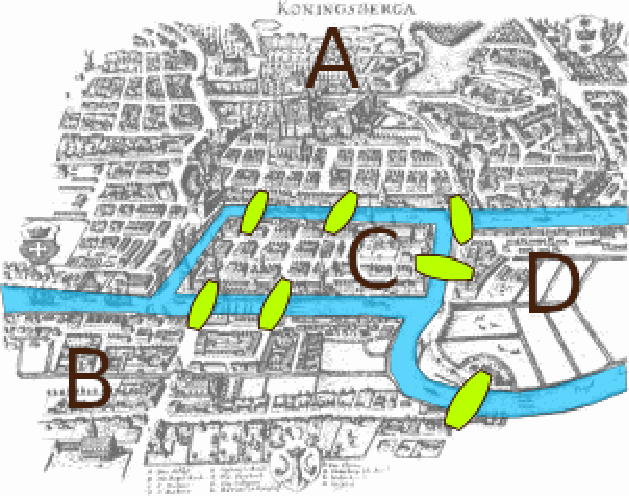
\includegraphics{./Figuras/Introduccion-a-grafos/Konigsberg_bridges.pdf}
\captionof{figure}{Los siete puentes de Königsberg.}
\end{center}

Viajamos a Prusia, siglo XVIII, a la ciudad de Königsberg. La gente de la ciudad se preguntaba si se podía partir de un punto $x \in A$ o $B$ de la ciudad, cruzar cada puente exactamente una sola vez y volver a $x$. Euler se propuso responder esta pregunta.

Podemos modelar el problema como un \textit{multi}grafo (i.e. dos vértices pueden estar unidos por más de una arista):

\Inkscape{Multigrafo de los puentes de Königsberg.}{"Figuras/Introduccion-a-grafos/Dibujo 31.pdf_tex"}


\begin{Definition}
Un \textbf{paseo} en un multigrafo, es una secuencia de vértices $x_0,x_1,\ldots, $ tal que $x_i x_{i+1}$ es arista para todo $i \geq 0$, y ninguna de estas aristas se repite (pero los vértices se pueden repetir) Un \textbf{paseo cerrado} es un paseo que comienza y termina en el mismo vértice. Un paseo es \textbf{Euleriano} si es cerrado y recorre todas las aristas del multigrafo. Un \textbf{(multi)grafo Euleriano}, es un (multi)grafo que contiene un paseo Euleriano.
\end{Definition}






%%%%%%%%%%%
\Clase{30/03/23}   %%%%%%%%%%%%%%%%%%%%%%%%%%%%%%%%%%%%%%%%%%%%%%%%%%%%%%%%%%%%%
%%%%%%%%%%%



\begin{Theorem}\label{th:paseo Euleriano si todos los vertices del multigrafo tienen grado par}
Un multigrafo conexo es Euleriano si y solo si todos sus vértices tienen grado par.
\end{Theorem}
\begin{proof}
\begin{enumerate}
\item[]


\item[($\Rightarrow$)] Asumimos que $G$ tiene un paseo Euleriano $P$. Cada vez que el paseo ``entra'' en una vértice, lo hace por medio de una arista, y debe ``salir'' por otra. Cada vez que $v$ a parece en $P$ se utilizan otras dos aristas incidentes en $v$. Como se ocupan todas esas aristas, $d(v)$ es par.

\item[($\Leftarrow$)]  Supongamos que todos los grados son pares. Haremos inducción en $\Abs G$. El caso base es $\Abs G = 2$ que claramente tiene un paseo Euleriano. Supongamos que $\Abs G >2$. Cuando todos los grados son pares, puedo encontrar un paseo cerrado no trivial. Tomemos como $P$ el de largo máximo, y sea $F$ su conjunto de aristas. Si $F$ es todo, la demostración está terminada. Luego supongamos que no. Sea $G':= G \setminus F$, tiene una arista $e$ que incide en un vértice de $P$. Sea $C$ la componente de $G'$ que contiene a $e$. Todo vértice de $G$, posee un número par de aristas incidentes en $F$, luego la cantidad de aristas en $G'$ sigue siendo par. Aplicando la hipótesis inductiva, podemos encontrar un paseo Euleriano en $C$, llamémoslo $P'$. Como $P$ y $P'$ unidos son un paseo cerrado más grande que $P$, llegamos a un absurdo.

\Inkscape{Ilustración de un grafo conexo $G$ con vértices de grado par, junto con un camino \black{negro} $P$ que no cubre todas las aristas de $G$, pero tal que existe una arista $e\in G \setminus V(P)$ que incide en $P$, donde la componente conexa $\blue{C}$ de $G \setminus V(P)$ conteniendo $e$ es un grafo Euleriano.}{"Figuras/Introduccion-a-grafos/Dibujo 32.pdf_tex"}
\end{enumerate}
\end{proof}

\begin{exercise}
Resolver el problema de los siete puentes de Königsberg.
\end{exercise}






\subsection{Conexidad}

\begin{Definition}
Sea $G$ un grafo con conjunto de vértices $V$. Decimos que un conjunto $X$ de vértices o aristas \textbf{separa} a $u,v \in V$ si $u,v \not \in X$ y todo camino entre $u$ y $v$ tiene un elemento de $X$.

Si $X$ separa un par de vértices, decimos que es \textbf{separador} (de $u,v$). Si un vértice solo, i.e. $X$ es un singleton, es separador, decimos que es un \textbf{vértice de corte}. Un pequeño abuso de notación será simplemente referirnos a ese vértice en lugar del conjunto que lo contiene.

Análogamente, una arista sola $X = \{e\}$ que separa sus vértices se dice \textbf{puente}. Un pequeño abuso de notación será simplemente referirnos a ese vértice en lugar del conjunto que lo contiene.
\end{Definition}

\Inkscape{Ejemplo: \yellow{$X = \{x_1,x_2,x_3,x_4,x_5 \}$} separa a \red{$u,v$}. Además, \purple{$Y = \{ e_1, e_2 \}$} e \brown{$Y ' = \{ e_3, e_4\}$} son separadores de \red{$u,v$}. Y por último, la arista \blue{$e$} es un puente.}{"Figuras/Introduccion-a-grafos/Dibujo 33.pdf_tex"}

\begin{definition}
Para $k \geq 0$ decimos que $G = (V,E)$ es \textbf{$k$-conexo} si $\abs V > k$ y $G \setminus X$ es conexo para todo $X \subset V$ con $\abs X < k$. Es decir, ningún conjunto de menos de $k$-vértices separa.
\end{definition}

\begin{example}
\begin{enumerate}[(a)]
\item Todo grafo no vacío es $0$-conexo.
\item Los grafos conexos con al menos una arista son $1$-conexos.
\end{enumerate}
\end{example}


\begin{definition}
La \textbf{conexidad}, $\Kappa (G)$ de $G$, es el máximo $k \geq 0$ tal que $G$ es $k$-conexo.
\end{definition}

\begin{example}\label{ex:clase6 - exemplo Kappa(K_n) = n-1}
\begin{enumerate}[(a)]
\item Los únicos grafos con $\Kappa (G) = 0$ son los grafos disconexos no triviales y $K_1$.
\item $\Kappa (K_n) = n-1$ para todo $n \in \naturals$.
\end{enumerate}
\end{example}

\begin{definition}
Sea $G$ no vacío y sea $\ell \geq 1$. Decimos que $G$ es \textbf{$\ell$-arista conexo}, si $G \setminus F$ es conexo para todo $F \subset E$ con $\Abs F < \ell$.
\end{definition}

\begin{example}
Los grafos conexos no vacíos son $1$-arista conexos.
\end{example}

\begin{definition}
La \textbf{arista conexidad}, $\lambda (G)$ de $G$, es el máximo $\ell$ tal que $G$ es $\ell$-arista conexo.
\end{definition}

\Inkscape[][triangulo azul de arriba]{Ejemplo de grafo con $\Kappa = 4$ y $\lambda = 4$.}{"Figuras/Introduccion-a-grafos/Dibujo 34.pdf_tex"}

\begin{example}\label{ex:clase6 - exemplo lambda (K_n) = Kappa(K_n) = n-1}
Se tiene que $\lambda (K_n) = n-1 , \forall n \geq 1$. Con lo cual, por el Ejemplo \ref{ex:clase6 - exemplo Kappa(K_n) = n-1},
$$
\lambda (K_n) = \Kappa (K_n) .
$$
\end{example}

\begin{exercise}
Calcular $\Kappa$ y $\lambda$ del siguiente grafo $G$:
\Inkscape*{}{"Figuras/Introduccion-a-grafos/Dibujo 35.pdf_tex"}
\end{exercise}
\begin{solution}
Llamemos $u,v$ a los dos únicos vértices de grado $7$. Si quitamos $u,v$, entonces nos queda $G$ disconexo, luego $\Kappa (G) <3$. Si quito cualquier vértice, entonces el grafo sigue siendo conexo, luego es $2$-conexo, i.e. $\Kappa (G) \geq 2$. Luego $\Kappa (G) = 2$.

En el anterior ejemplo \ref{Figura:triangulo azul de arriba} teníamos $\lambda = 4$ en cada \blue{triángulo azul}, y como sacar $3$ aristas incidentes a $u,v$ no evita que $G$ siga siendo conexo, tenemos que $G$ es $4$-arista conexo, i.e. $\lambda (G) \geq 4$. Por otro lado, si quitamos las $4$ aristas incidentes alguno de los vértices del \red{triángulo rojo}, queda aislado del resto del grafo, i.e. $\lambda (G) < 5$. Luego $\lambda (G) = 4$.
\end{solution}


%%%%%%%%%%%
\Clase{03/04/23}   %%%%%%%%%%%%%%%%%%%%%%%%%%%%%%%%%%%%%%%%%%%%%%%%%%%%%%%%%%%%%
%%%%%%%%%%%

\begin{Proposition}\label{proposition:desigualdad que relaciona numero de conexion numero arista conexion y grado minimo}
Si $G$ es no trivial, entonces $\Kappa (G) \leq \lambda (G) \leq \delta (G)$.
\end{Proposition}
\begin{proof}
La segunda desigualdad se tiene porque todas las aristas incidentes en un vértice fijo separan a $G$.

Veamos ahora la primera desigualdad. Sea $F$ un conjunto de aristas que separa a $G$, con $\abs F = \lambda (G)$, tal que $G \setminus F$ es disconexo. \textit{Observación:} $F$ es un conjunto de aristas minimal con la propiedad de ser separador.

\textbf{Caso 1:} Existe $v \in V(G)$ que no incide en $F$. Sea $C$ la componente conexa que contiene a $v$ en $G \setminus F$. No puede haber una arista $f$ de $F$ con ambos extremos en $C$, pues de lo contrario $F \setminus \{f\}$ sería un conjunto separador más chico, contradiciendo la minimalidad de $F$. (Ver la siguiente figura \ref{Figura:ilustracion de C y F violeta}). Luego, si quitamos los vértices de las aristas de $F$ incidentes en $C$, las cuales solo comparten un vértice con $C$, nos queda que $v$ estaría separado del resto del grafo. Esta cantidad de vértices es a lo sumo $\abs F = \lambda (G)$. Con lo cual $\Kappa (G) \leq \abs F = \lambda (G)$.

\Inkscape[][ilustracion de C y F violeta]{Ilustración de la componente \blue{$C$} que contiene a $v$, donde las \purple{aristas violeta} corresponden a un conjunto separador $\purple{F}$. Notar que en este ejemplo \purple{$F$} no es minimal, pues $\purple {f \in F}$ tiene ambos extremos en \blue{$C$}.}{"Figuras/Introduccion-a-grafos/Dibujo 36.pdf_tex"}

\textbf{Caso 2:} Todo $v \in V(G)$ incide en $F$. Fijemos $v \in V(G)$ y $C$ la componente conexa de $G \setminus F$ que lo contiene. Consideremos $N_{G} (v)$, los vecinos de $v$. Cada $w \in N_{G} (v) $ incide en una arista de $F$. (Ver la siguiente Figura \ref{Figura:los vecinos de v inciden en al menos una arista de F}). Entonces $d_G (v) \leq \abs F = \lambda (G)$. Por lo tanto, salvo que $V(G) = \{ v \} \cup N_G ( v)$, tenemos que $N_G (v)$ separa a $v$ del resto del grafo, y salvo ese caso tendríamos que $\Kappa (G) \leq \abs{N_G (v)} \leq \lambda (G)$. Pero $v$ era arbitrario, entonces en el peor de todos los casos, tenemos que $V(G) =  \{ v \} \cup N_G ( v)$ para todo $v \in G$, i.e. $G$ es un grafo completo. Afortunadamente, vale la igualdad por el Ejemplo \ref{ex:clase6 - exemplo lambda (K_n) = Kappa(K_n) = n-1}. Esto concluye la demostración de la primera desigualdad.

\Inkscape[][los vecinos de v inciden en al menos una arista de F]{Ilustración de lo que sucede: los \darkgreen{vecinos} de \green{$v$} inciden en al menos una \purple{arista de $F$}.}{"Figuras/Introduccion-a-grafos/Dibujo 37.pdf_tex"}
\end{proof}

\subsection{Grafos $2$-conexos}

\begin{Definition}
Sea $H$ un grafo. Decimos que un camino $P$ es un \textbf{$H$-camino} si es no trivial (tiene al menos una arista) e interseca a $H$ exactamente en sus extremos ($P$ no tiene ni vértices ni aristas en $H$, salvo por sus extremos).
\end{Definition}

\Inkscape{Ejemplo de \blue{$H$}-camino \yellow{$P$}. Notar que en el dibujo consideramos a los vértices \blue{$x,y$} como extremos de \yellow{$P$}.}{"Figuras/Introduccion-a-grafos/Dibujo 38.pdf_tex"}

Los ciclos son los grafos $2$-conexos más elementales. De hecho, veamos que todos los demás grafos $2$-conexos se pueden construir a partir de ellos.

\begin{proposition}\label{prop:un grafo es 2-conexo si y solo si se construye a partir de un grafo 2-conexo union un H-camino}
Un grafo es $2$-conexo si y solo si se puede construir a partir de un ciclo añadiendo sucesivamente $H$-caminos a grafos $H$ ya construidos.
\end{proposition}

\begin{remark}
Es decir, si $H_0$ es un ciclo, le agregamos un $H_0$-camino, y a la unión la llamamos $H_1$, el cual es $2$-conexo; si quisieramos podemos agregar un $H_1$-camino y seguiría siendo $2$-conexo, etc. Más formalmente, un grafo $G$ es $2$-conexo, si y solo si existe una secuencia de grafos
\[
H_0 \subset H_1 \subset \cdots \subset H_n, \quad n \geq 1,
\]
tal que $H_0$ es un ciclo, $H_n = G$, y $H_{i+1}$ se obtiene a partir de $H_{i}$ agregando un $H_{i}$-camino. Ver la siguiente figura:

\Inkscape{Ilustración de la secuencia $\darkgreen{H_0} \subset \yellow{H_1} \subset \red{H_2} \subset \blue{H_3}$.}{"Figuras/Introduccion-a-grafos/Dibujo 39.pdf_tex"}
\end{remark}

\begin{proof}[Demostración de la proposición]
\begin{enumerate}
\item[]

\item[($\Leftarrow$)] Claramente un grafo construido de esta manera no se puede separar por un solo vértice. Y por su puesto que tiene más de $2$ vértices. Con lo cual es $2$-conexo.

\item[($\Rightarrow$)] Tomemos un grafo $G$, $2$-conexo (en particular es también conexo). Como es $2$-conexo, debe tener algún ciclo $C$, pues de lo contrario sería un árbol con al menos $3$-vértices, y quitando un vértice que no es hoja nos quedaría separado por el ítem (iv) de \ref{theorem:caracterizacion de arbol}.

Ahora nos fijamos si tiene un $C$-camino, si esto es así lo agregamos, y luego seguimos agregando hasta que no podamos más. Consideremos el subgrafo maximal $H$ de $G$ construido de esta manera a partir de $C$. Entonces toda arista $xy \in E(G) \setminus E(H)$ tal que $x,y \in V(H)$, es un $H$-camino, con lo cual no puede existir por maximalidad de $H$. Es decir, $H$ es un subgrafo inducido de $G$. Entonces todas las aristas de $G$ que no están en $H$ tienen un extremo fuera de $H$. Si $H$ es $G$ habríamos terminado, luego por el absurdo supongamos que no. Por conexión existe un vértice $v \in G \setminus H$, y conectándolo por un camino con $H$ podemos asumir que $v$ es incidente en $H$, es decir, existe $w \in H$ tal que $v w$ es una arista incidente en $H$. Como $G$ es $2$-conexo, si quitamos $w$, el grafo sigue siendo conexo, por lo tanto debe ser que existe otro camino $P$ de $v$ a $H$ que no contiene a $w$, con lo cual $P \cup v w$ es un $H$-camino. Sin embargo, esto es absurdo por maximalidad de $H$. Ver la siguiente ilustración:

\Inkscape*{}{"Figuras/Introduccion-a-grafos/Dibujo 40.pdf_tex"}
\end{enumerate}
\end{proof}










%%%%%%%%%%%
\Clase{06/04/23}   %%%%%%%%%%%%%%%%%%%%%%%%%%%%%%%%%%%%%%%%%%%%%%%%%%%%%%%%%%%%%
%%%%%%%%%%%




Todo grafo \textit{sin vértices aislados} se puede particionar en subgrafos $1$-conexos. Y podemos intentar nuevamente caracterizar los grafos $2$-conexos. Sin embargo, nos topamos con problemas, por ejemplo:

\Inkscape[][problemas la definicion de subgrafo 2-conexo maximal y bloques]{Los subgrafos $2$-conexos maximales de este grafo son sus ciclos, los cuales comparten vértices entre sí y con otras estructuras como las aristas que inciden en \red{$v$}.}{"Figuras/Introduccion-a-grafos/Dibujo 41.pdf_tex"}

Como ilustra la figura de arriba, los subgrafos $2$-conexos maximales no siempre abarcan todo el grafo ni son siempre disjuntos. La siguiente definición viene a solucionar esto:

\begin{definition}
Un \textbf{bloque} es un subgrafo conexo maximal sin vértices de corte.
\end{definition}

En la Figura \ref{Figura:problemas la definicion de subgrafo 2-conexo maximal y bloques}, los bloques del grafo con los \blue{ciclos} y las \red{aristas} (junto con sus extremos) que inciden en \red{$v$}.

\begin{obs}
Es fácil ver que los bloques van a ser o subgrafos \textit{$2$-conexos} o una \textit{arista} o un \textit{vértice}.
\end{obs}

\begin{proposition}
Los ciclos de un grafo son los ciclos de sus bloques.
\end{proposition}
\begin{proof}
Todo ciclo es $2$-conexo, luego es conexo sin vértices de corte, y debe estar contenido en un subgrafo maximal con esta propiedad, i.e. un bloque.
\end{proof}

\begin{proposition}
Sean $e,f \in E(G)$. Entonces pertenecen a un mismo bloque si y solo si pertenecen a un mismo ciclo.
\end{proposition}
\begin{proof}
Si pertenecen al mismo ciclo, entonces por la proposición anterior están en un mismo bloque.

Recíprocamente, como $e,f$ son dos aristas en un mismo bloque, puedo asumir que el bloque es un subgrafo $2$-conexo (no es arista sola o vértice solo). La idea es la siguiente: este subgrafo $2$-conexo se construye a partir de un ciclo uniendo $H$-caminos por la Proposición \ref{prop:un grafo es 2-conexo si y solo si se construye a partir de un grafo 2-conexo union un H-camino}, luego no es difícil ver que las dos aristas están contenidas en un mismo ciclo.
\end{proof}

\begin{definition}
El \textbf{grafo bloque} de un grafo conexo $G$, denotado por $\block G$, es el grafo que tiene un vértice por cada bloque y por cada vértice de corte de $G$; y $Xy$ es una arista de $\block G$ si $X$ es un bloque e $y$ es un vértice de corte de $G$ contenido en $X$.
\end{definition}

\Inkscape{Del lado izquierdo se ilustra $G$, que tiene $5$ bloques: \blue{$A$}, \yellow{$B$}, \red{$C$}, \purple{$D$}; y $2$ \darkgreen{vértices de corte}. Del lado derecho se ilustra $\block G$.}{"Figuras/Introduccion-a-grafos/Dibujo 42.pdf_tex"}

Notar que en nuestro ejemplo, el grafo bloque es un árbol. Esto no es casualidad:

\begin{exercise}\label{exercise:el grafo bloque de un grafo conexo es un arbol}
El grafo bloque de un grafo conexo es un árbol.
\end{exercise}
\begin{proof}
\textit{Notación:} a los bloques de $G$ los denotamos por letras mayúscula, y a los vértices de corte los denotamos por una letra minúscula. Utilizaremos la misma notación y términologia para referirnos a los respectivos vértices en el grafo bloque $\block G$; quedará claro dependiendo del contexto, a qué grafo pertenece cada vértice en esta notación. En particular, un bloque de $\block G$ es un vértice que corresponde a un bloque de $G$, y similarmente un vértice de corte de $\block G$ es un vérticce que corresponde con uno de $G$.

Primero veamos que $\block G$ es conexo. Para eso, basta probar que entre dos bloques de $\block G$ existe un camino, pues todo vértice de corte de $\block G$ es adyacente a algún bloque en $\block G$ por definición de grafo bloque. Sean $B,B'$ dos bloques de $\block G$, consideremos un $B,B'$-camino $P$ en $G$, el cual se puede tomar de tal suerte que no puede entrar y salir de un bloque más de una vez. Este camino nos induce un camino en $\block G$ dado por $\tilde P : B_0 v_0 B_1 v_1 \cdots B_{r-1} v_{r-1} B_r $, donde cada bloque o vértice aparece en el orden en el cual el camino $P$ se intersecó por primera véz con este.

Ahora veamos que $\block G$ es aciclico. En efecto, supongamos que no, sea $C$ un ciclo en $\block G$. Como $\block G$ es bipartito (se puede particionar: vértices de corte y bloques), no tiene ciclos impares, luego $C$ tiene al menos $4$ vértices. Con lo cual, existen dos bloques distintos $B_1,B_2$ y dos vértices de corte distintos $v_1,v_2$ tales que $C = B_1 v_1 B_2 \cdots v_2 B_1$. Pero esto quiere decir que podemos quitar $v_1$ de $G$ y sigue siendo conexo, i.e., $v_1$ no era vértice de corte, absurdo.
\end{proof}


\subsection{Contracciones y menores}

\begin{definition}
\textbf{Contraer una arista} $e=xy$ equivale a borrar $x$ e $y$, y añadir un nuevo vértice $v_{xy}$ adyacente a todos los vértices que eran vecinos a $x$ o $y$.
\end{definition}

\begin{notation}
Dado un grafo $G$ y $e = xy \in E(G)$, notamos como $G/e$ al grafo que se obtiene de $G$ al contraer la arista $e$.
\end{notation}

\Inkscape{Contracción de los vértices \blue{$x,y$} de un grafo $G$. Forma el vértice $\blue{v_{xy}}$ de $G/xy$.}{"Figuras/Introduccion-a-grafos/Dibujo 43.pdf_tex"}

\begin{definition}
Decimos que un grafo $H$ es un \textbf{menor} de $G$ si se puede obtener a partir de $G$ utilizando las siguientes operaciones:
\begin{enumerate}[1.]
\item borrar vértices,
\item borrar aristas,
\item contraer aristas. (Equivalentemente, contraer subgrafos conexos).
\end{enumerate}
\end{definition}

\begin{example}
Los subgrafos y contracciones de $G$ son \textit{menores} de $G$. No necesariamente vale la vuelta:

\Inkscape{Ejemplo de menor $H$ de un grafo $G$, que no es subgrafo, ya que tiene un vértice de grado $5$. Notar que $H$ se obtiene luego de contraer las \red{aristas rojas} de $G$.}{"Figuras/Introduccion-a-grafos/Dibujo 44.pdf_tex"}
\end{example}


\subsection{Subdivisiones}\label{subsection: subdivisiones}

Sea $X$ un grafo fijo.

\begin{definition}
Llamamos \textbf{subdivisión} de $X$ a cualquier grafo $G$ que se obtiene de \textit{subdividir} algunas aristas de $X$ y dibujando encima nuevos vértices. Más precisamente, reemplazamos las aristas de $X$ con nuevos caminos entre sus extremos, de manera que estos caminos no se intersecan entre si y tampoco intersecan a $V(X)$ salvo en los extremos.
Diremos que $G$ es un $TX$.

Llamaremos a los vértices originales de $X$, \textbf{vértices de ramificación de los de} $TX$; a los nuevos vértices los llamaremos \textbf{vértices subdivisores}. (Notar que los vértices subdivisores tienen grado $2$ y los vértices de ramificación no cambian de grado).

Si un grafo $Y$ contiene a $TX$ como subgrafo, diremos que $X$ es un \textbf{menor topológico}\footnote{
En topología el número de ``agujeros'' de un espacio topológico $X$ es un invariante topológico, más precisamente, es invariante por \textit{homotopías} (deformaciones continuas del espacio). Por ejemplo, un triángulo tiene $1$ agujero, pero dos triángulos adyacentes por una arista tiene $2$. En grafos también podemos definir una ``noción de agujero'', y claramente si $X$ tiene $n$ agujeros, $TX$ también, pues no estamos agregando más! De aquí el nombre de menor \textit{topológico}. Notar que de todas formas, $Y$ puede tener más agujeros que $TX$, pues este último es solo un subgrafo.
} de $Y$.
\end{definition}

\Inkscape{De izquierda a derecha, construimos progresivamente $X$, luego le agregamos \red{vértices subdivisores} formando $TX$, y finalmente ilustramos un ejemplo de grafo $Y$ con $X$ como menor topológico.}{"Figuras/Introduccion-a-grafos/Dibujo 45.pdf_tex"}

\begin{definition}
Similarmente, reemplazando los vértices $x \in X$ con grafos conexos disjuntos $G_x$, y las aristas $xy \in X$ con conjuntos no vacíos de $G_x - G_y$ aristas, obtenemos un grafo que llamaremos $IX$. Recíprocamente, decimos que $X$ se obtiene a partir de $G$ \textbf{contrayendo} subgrafos $G_x$ (y fusionando las $G_x-G_y$ aristas), y lo llamamos una \textbf{menor contraida} de $G$.

Si un grafo $Y$ contiene un $IX$ como subgrafo, decimos entonces que $X$ es una \textbf{menor} de $Y$, llamamos a $IX$ un \textbf{modelo} de $X$ en $Y$, y notamos $X\preccurlyeq Y$.
\end{definition}

\Inkscape{De izquierda a derecha, tenemos el grafo $X$, que se obtiene de contraer los subgrafos \red{$G_x$}, \darkgreen{$G_y$}, \blue{$G_z$}, \purple{$G_w$} de $G$; finalmente, el grafo $Y$ tiene a $X$ como menor y a $G$ como modelo de $X$ en $Y$.}{"Figuras/Introduccion-a-grafos/Dibujo 46.pdf_tex"}

Por lo tanto, $X$ es un menor de $Y$ si y solo si existe una función $\varphi : S \subset V(Y) \twoheadrightarrow V(X)$ tal que para todo vértice $x \in X$ si preimagen $\varphi^{-1} (x)$ es conexa en $Y$ y para toda arista $xx' \in E(X)$ existe una arista en $Y$ entre conjuntos de ramificación $\varphi^{-1}(x), \varphi^{-1} (x')$. Si el dominio de $\varphi$ es todo $V(Y)= S$, y si $xx' \in E(X)$ siempre que $x \neq x'$ e $Y$ tiene una arista entre $\varphi^{-1}(x)$ y $\varphi^{-1} (x')$, es decir $Y$ es una $IX$, decimos que $\varphi$ es una \textbf{contracción} de $Y$ en $X$.


\begin{obs}
La relación de menores $\preccurlyeq$ y la relación de menores topológicos son ordenes parciales en la clase de grafos finitos. Es decir, son reflexivos, antisimétricos, y transitivos.
\end{obs}


Si $G$ es una $IX$, luego $P = \Set{G_x | x \in X}$ es una partición de $V(G)$, y notamos $G/P := X$. Si $U = G_x$ es el único conjunto de ramificación que no es un singleton, escribimos $G/U := X$, y notamos $v_U$ al vértice $x \in X$ al que se contrae $U$, y pensamos al ressto de $X$ como un subgrafo inducido de $G$. El caso más simple es cuando $U$ contiene exactamente dos vértices que forman una arista $e= U$, aquí escribiremos $G/e = X$.

\begin{proposition}
Sean $X$ e $Y$ do grafos. Entonces $X$ es una menor de $Y$ si y solo si existen grafos $G_0,\ldots,G_n$ tales que $G_0 = Y$ y $G_n = X$, y además $G_{i+1}$ se obtiene a partir de $G_i$ borrando aristas, contrayendo aristas, o borrando vértices.
\end{proposition}
\begin{proof}
Estas tres últimas operaciones claramente producen una menor $X$, pues la relación de menor es transitiva. Recíprocamente, se puede hacer inducción en $\abs Y + \Abs Y$.
\end{proof}

Finalmente, tenemos la siguiente relación entre menores y menores topológicos:

\begin{proposition}
\begin{enumerate}[(i)]
\item Todo $TX$ es también un $IX$ (ver la Figura \ref{Figura:subdivision de K4 visto como IK4}). Por lo tanto, todo menor topológico de un grafo es un menor de él.
\item Si $\Delta (X) \leq 3$, entonces todo $IX$ contiene un $TX$. Con lo cual, todo menor con grado máximo a lo sumo $3$ de un grafo es también un menor topológico de él.
\end{enumerate}
\end{proposition}
\begin{proof}
Veamos solo (ii), el primer ítem es obvio. $IX$ es el grafo que se obtiene de $X$ reemplazando cada vértice $x$ de él por un subgrafo conexo $G_x$ y cada arista por un conjunto de aristas no vacío, luego tomando una arista de ese conjunto, basta con escoger un vértice de $G_x$ que tenga por cada vecino de $x$ en $X$ un camino distinto hacia cada arista incidente en $G_x$, y con interiores disjuntos entre sí. Esto es posible: empezamos eligiendo de manera inocente al vértice que es extremo de una arista incidente con $G_x$, llamemosló $x$, de este vértice tendríamos que encontrar dos caminos internamente disjuntos con extremos en otras dos aristas incidentes a $G_x$, pues $\Delta X \leq 3$. Ahora, dos caminos siempre existen, con lo cual si no se cruzan ganamos, pero si se cruzan, lo hacen a partir de un momento, incluso varias veces. En este caso, movemos nuestro vértice $x$ a la última véz que se cruzan los caminos, y llamemosló $x'$. Esto funciona:

\Inkscape*{Ilustración de cómo se ven dos caminos, ambos de color amarillo pero uno más claro que el otro, que salen de nuestro vértice $x$ y tienen que llegar a las aristas incidentes en $G_x$. Al final movemos nuestro vértice a $x'$.}{"Figuras/Introduccion-a-grafos/Dibujo 47.pdf_tex"}
\end{proof}

\Inkscape[][subdivision de K4 visto como IK4]{Subdivisión de $K_4$ visto como $IK_4$.}{"Figuras/Introduccion-a-grafos/Dibujo 48.pdf_tex"}

\begin{definition}
Una \textbf{incrustación} o \textbf{inmersión} (en inglés \textbf{embedding}) de un grafo $H$ en un grafo $G$, es una función inyectiva $\varphi : V(H) \rightarrow V(G)$ que preserva la estructura en la que estamos interesados. En particular:
\begin{enumerate}[(a)]
\item $\varphi$ incrusta a $H$ en $G$ como \underline{subgrafo} si preserva la adyacencia entre vértices;
\item y como \underline{subgrafo inducido} si preserva tanto la adyacencia como la no adyacencia;
\item si $\varphi$ está definido también en $E(H)$ como en $V(H)$ y manda $xy$ en caminos independientes de $G$ entre $\varphi (x)$ y $\varphi (y)$, decimos que $\varphi$ incrusta a $H$ en $G$ como \underline{menor topológico};
\item similarmente, decimos que es una incrustación de $H$ en $G$ como \underline{menor}, si mapea a $V(H)$ en subgrafos conexos disjuntos de $G$, de manera que $G$ tiene una arista entre los conjuntos $\varphi (x)$ y $\varphi (y)$ siempre que $xy \in E(H)$.
\end{enumerate}
Existen más variantes, pero dependen del contexto en el que estemos; por ejemplo, se pueden definir de manera obvia las incrustaciones de ``subgrafos generadores'', ``menores inducidas'', etc.
\end{definition}

%%%%%%%%%%%
\Clase{17/04/23}   %%%%%%%%%%%%%%%%%%%%%%%%%%%%%%%%%%%%%%%%%%%%%%%%%%%%%%%%%%%%%

%%%%%%%%%%%


\begin{lemma}\label{lema:todo grafo 3-conexo distinto de K_4 tiene una arista e tal que G/e es nuevamente 3-conexo}
Todo grafo $3$-conexo, distinto de $K_4$, tiene una arista $e$ tal que $G/e$ es $3$-conexo.
\end{lemma}
\begin{proof}
Supongamos por el absurdo que no existe una arista $e$ con esta propiedad. Es decir, para toda arista $e = xy \in E(G)$, el grafo $G/e$ tiene un conjunto separador $S$ con a lo más $2$ vértices. Como $G$ es $3$-conexo, $v_{xy}$ (el vértice que sale de contraer la arista $xy$) tiene que estar en $S$, además $\abs S = 2$. En efecto, $\abs S = 0$ es imposible porque el grafo es conexo, por otro lado, si $\abs S = 1$, estamos diciendo que $G$ se puede separar con un solo vértice si $v_{xy} \not \in S$, o que $G$ se puede desconectar removiendo $x,y$ si $v_{x,y} \in S$, en cualquier caso esto no ocurre.

Luego, escribimos $S = \{z, v_{xy}\}$ con $z \not \in \{x,y\}$ (que depende de $x,y$) para el conjunto separador de $G/xy$ del párrafo anterior. Con lo cual, $T=\{z,x,y\}$ separa a $G$. Como ningún subconjunto propio de $T$ separa $G$, cada vértice de $T$ tiene un vecino en cada componente de $G \setminus T$.

Como $xy$ era arbitrario, podemos elegir la arista $xy$, tal que existe $z$ como arriba, de tal forma que $G \setminus T$ tenga una componente $C$ más chica posible. Tomo $v \in C$; es vecino de $z$. Entonces $G/v z$ tampoco es $3$-conexo, o sea que como antes, existe $w$ tal que $v,z,w$ separan $G$. Nuevamente, cada vértice $v,z,w$ tiene un vecino en cada componente de $G \setminus \{v,z,w\}$. Como $x$ e $y$ son adyacentes, existe $D$ componente de $G \setminus \{v,z,w\}$ tal que $D \cap \{x,y\} = \emptyset$ (porque $G \neq K_4$). Dado que $v \in C$, los vecinos de $v$ en $D$ están en $C$. Tenemos que $D \cap C \neq \emptyset$, más aún, $D \subsetneq C$. Contradiciendo la minimalidad del orden de $C$. Esto concluye la demostración por el absurdo.
\end{proof}

\begin{Theorem}[Teorema de Tutte, 1961]
Un grafo $G$ es $3$-conexo si y solo si existe una secuencia de grafos $G_0, G_1, \ldots, G_n$ que cumple lo siguiente:
\begin{enumerate}[(i)]
\item $G_0 = K_4$ y $G_n = G$.
\item $G_{i+1}$ tiene una arista $xy$ tal que $d(x),d(y) \geq 3$ y $G_i = G_{i+1}/xy$ para todo $i < n$. Más aún, cada $G_i$ es $3$-conexo.
\end{enumerate}
\end{Theorem}
\begin{proof}
Notar que aplicando recursivamente el lema anterior podemos encontrar una secuencia de grafos $3$-conexos, $G_0, G_1, \ldots, G_n$ tales que $G_0 = K_4$ (es el único grafo $3$-conexo de orden $4$) y $G_n = G$, de tal suerte que $G_{i} = G_{i+1}/e_i$ para alguna arista $e_i \in G_{i+1}$ ($i < n$). Notar que el Teorema \ref{proposition:desigualdad que relaciona numero de conexion numero arista conexion y grado minimo} implica que el grado de $x,y$ es al menos $3$. La recíproca es trivial.
\end{proof}


%%%%%%%%%%%
\Clase{20/04/23}   %%%%%%%%%%%%%%%%%%%%%%%%%%%%%%%%%%%%%%%%%%%%%%%%%%%%%%%%%%%%%
%%%%%%%%%%%

\subsection{Teorema de Menger}
\begin{definition}
Si $A,B,X \subset V(G)$ son tales que todo $A,B$-camino tiene un vértice de $X$, decimos que $X$ separa a $A$ y $B$ en $G$.
\end{definition}

\begin{theorem}[Menger, 1927]\label{theorem:teorema de menger}
Sea $G = (V,E)$ un grafo y sean $A,B \subset V$. El mínimo número de vértices que separa a $A$ y $B$ es igual al máximo número de $A,B$-caminos disjuntos.
\end{theorem}
\begin{proof}
Sea $k$ el mínimo número de vértices que separan $A$ y $B$. Como no pueden haber más $A,B$-caminos disjuntos que vértices de un conjunto que separa $A$ y $B$, se sigue que el número máximo número de $A,B$-caminos disjuntos es a lo más $k$.

\Inkscape*{}{"Figuras/Introduccion-a-grafos/Dibujo 49.pdf_tex"}

Para la otra desigualdad, haremos inducción en el número de aristas. Si $G$ no tiene aristas entonces los $A,B$-caminos son puntos de $A \cap B$, con lo cual vale la igualdad. Ahora, si existe una arista $e = xy$ de $G$, y si $G$ no tiene $k$ caminos entre $A,B$ disjuntos (es decir tiene $<k$), entonces $G/e$ tampoco (¿por qué?). Luego por hipótesis inductiva, $G/e$ tiene un $A,B$-separador $Y$ con menos de $k$ vértices. El vértice $v_e$ debe estar en $Y$, porque si no $Y$ sería separador de $G$, contradiciendo minimalidad de $k$. Consecuentemente, $X = (Y \setminus \{v_e\}) \cup \{x,y\}$ es un $A,B$-separador de $G$ con exactamente $k$ vértices. En efecto, por minimalidad $k \leq \abs X$, y por construccón $\abs X = \abs Y + 1 < k +1 \leq k$.

Consideremos ahora $G \setminus e$. Todo $A,X$-separador en $G \setminus e$ es un $A,B$-separador en $G$ con al menos $k$-vértices por minimalildad de $k$ (ver la siguiente Figura \ref{Figura:AX separador de G menos e es un AB separador en G}). Por inducción, hay al menos $k$ caminos entre $A,X$ disjuntos en $G \setminus e$. Lo mismo pasa con los $B,X$-caminos. Como $X$ separa a $A$ y $B$, estos caminos solo se encuentran en $X$ y los puedo combinar para tener al menos $k$ caminos disjuntos entre $A$ y $B$, contradicción.

\Inkscape[][AX separador de G menos e es un AB separador en G]{Ilustración del conjunto separador \brown{$X$} y los conjuntos de vértices \red{$A$} y \blue{$B$}. Notar que todos los $A,B$-caminos deben pasar por el \yellow{$A,X$-separador}.}{"Figuras/Introduccion-a-grafos/Dibujo 50.pdf_tex"}
\end{proof}

\begin{definition}
El \textbf{grafo línea} $L(G)$ de un grafo $G = (V,E)$ es aquel cuyo conjunto de vértices es $E$ y $ef$ es una arista de $L(G)$ si y solo si $e$ y $f$ comparten un extremo en $G$.
\end{definition}

\Inkscape{Ejemplo de un grafo $G$ y su grafo línea $L(G)$.}{"Figuras/Introduccion-a-grafos/Dibujo 51.pdf_tex"}

\begin{definition}
Sea $a$ un vértice y $B$ un conjunto de vértices. Un conjunto de $a,B$-caminos de dice \textbf{$a,B$-abanico} si cada par de estos caminos se intersecan solamente en $a$.
\end{definition}

\Inkscape{Ejemplo de $\red{a},\blue{B}$-abanico.}{"Figuras/Introduccion-a-grafos/Dibujo 53.pdf_tex"}

\begin{corollary}
Para $B \subset V$ y $a \in V \setminus B$, el mínimo número de vértices que separan $a$ de $B$ en $G$ es igual al máximo número de caminos en un $a,B$-abanico en $G$.
\end{corollary}
\begin{proof}
Aplicamos el Teorema de Menger \ref{theorem:teorema de menger} al grafo $G \setminus a$ con conjuntos $A := N_G (a)$ y $B$. Así obtenemos el corolario.

\Inkscape{Ilustración del procedimiento: en \red{rojo} los \red{vecinos} de $a$, en \blue{azúl} el conjunto \blue{B}, y en \brown{marrón} un connjunto $\red{A},\blue{B}$-separador \brown{$X$}.}{"Figuras/Introduccion-a-grafos/Dibujo 54.pdf_tex"}
\end{proof}

\begin{corollary}
Sean $a$ y $b$ vértices distintos de $G= (V,E)$. Entonces,
\begin{enumerate}[(i)]
\item Si $ab \not \in E$ ($a,b$ no son adyacentes), entonces el mínimo número de vértices que separan $a$ de $b$ en $G$ es igual al máximo número de $a,b$-caminos internamente disjuntos.
\item El mínimo número de aristas que separan $a$ de $b$ es igual al máximo número de $a,b$-caminos arista-disjuntos.
\end{enumerate}
\end{corollary}
\begin{proof}
\begin{enumerate}[(i)]
\item Aplicamos el Teorema de Menger \ref{theorem:teorema de menger} a $G \setminus \{a,b\}$ con $A := N_G (a)$ y $B := N_G (b)$.
\item Observemos que hay una correspondencia biyectiva entre aristas $A,B$-separadoras de $G$ y vértices separadores de $E(A),E(B)$ (los conjuntos de aristas incidentes en $A$ y $B$, respectivamente) en $L(G)$; y también entre los $A,B$-caminos arista-disjuntos de $G$ y los $E(A),E(B)$-caminos disjuntos de $L(G)$. Así, aplicamos el Teorema de Menger \ref{theorem:teorema de menger} al grafo línea $L(G)$ con conjuntos $A := E(a)$ y $B := E(b)$.
\end{enumerate}
\end{proof}

\begin{theorem}[Versión global de Menger]\label{th:version global de Menger}
\begin{enumerate}[(i)]
\item Un grafo $G$ es $k$-conexo si y solo si contiene $k$-caminos internamente disjuntos entre cada par de vértices.
\item Un grafo $G$ es $k$-arista conexo si y solo si contiene $k$ caminos arista disjuntos entre cada par de vértices.
\end{enumerate}
\end{theorem}
\begin{proof}
\begin{enumerate}[(i)]
\item Por un lado, si hay $k$ caminos internamente disjuntos entre cada par de vértices pero $G$ no es $k$-conexo, es porque existen dos vértices $x,y$ separados por un conjunto $X$ con $\abs X \leq k-1$, pero el ítem (i) del corolario anterior implica que hay a lo más $k-1$ caminos internamente disjuntos entre $x,y$, lo cual es absurdo. Recíprocamente, si $x,y$ son dos vértices no adyacente, el corolario anterior implica que hay al menos $k$ caminos internamente disjuntos entre $x,y$, pues si $G$ es $k$-conexo, el mínimo conjunto $x,y$-separador debe tener al menos $k$-vértices. Si $x,y$ son dos vértices adyacentes, el ítem (i) del corolario anterior sigue valiendo, solo que ahora hay más caminos arista disjuntos: hay que contar el camino $xy$.

\item El razonamiento es totalmente análogo al ítem anterior: aplicar el ítem (ii) del corolario de arriba.
\end{enumerate}
\end{proof}





\section{Ejercicios}

\begin{exercise}
Sea $G$ un grafo que contiene un ciclo $C$, y supongamos que $G$ contiene un camino de longitud al menos $k$ entre
dos vértices de $C$. Probar que $G$ contiene un ciclo de longitud al menos $\sqrt k$.
\end{exercise}
\begin{solution}
Si $C$ tiene longitud $\sqrt k$ entonces la afirmación vale. Si no, denotemos por $P$ al camino de longitud $k$
entre dos vérticces $x,y \in C$. Como $\Abs C < \sqrt k$, $P$ interseca con $C$ en menos de $\sqrt k$ vértices,
por lo tanto existen dos vértices $a,b \in P \cap C$ tales que, en el orden inducido por el camino $P$, no hay otro
vértice de $C$ entre estos, y $a P b$ tiene longitud $\geq \sqrt k$. Luego el ciclo $a P b C a$ tiene logitd $\geq \sqrt k$.
\end{solution}


\begin{exercise}
Probar que los grafos de cintura $\geq 5$ y orden $n$ tienen $\delta = o (n)$. Es decir, existe $f : \naturals \rightarrow \naturals$ tal que $f(n) /n \rightarrow 0$ cuando $n \rightarrow \infty$ y $\delta (G) \leq f(n)$ para todo $G$ de orden $n$.
\end{exercise}
\begin{solution}
En efecto, tenemos que
$$
n = \abs G \geq n_0 ( \delta, 5) = 1 + \delta (1 + (\delta -1)) = 1 + \delta^2
$$
por el Teorema débil \ref{th:version debil del teorema de Alon, Hoory y Lineal en 2002}, si $\delta \geq 2$.
\end{solution}



\begin{exercise}
Probar que todo grafo conexo $G$ con $\abs G \geq 3$ contiene un camino o un ciclo de longitud al menos $k := \min \{2 \delta (G) , \abs G\}$. (En general, vale para cualquier grafo conexo con $k = \min \{2 \delta (G), \abs G - 1\}$).
\end{exercise}
\begin{solution}
Tomemos $P := v_0, \ldots, ,v_l$ un camino de largo máximo en $G$. Sabemos que $N_G (v_0)$ y $N_G (v_l)$ están contenidos en $V(P)$ por maximalidad de $P$. Si $V(P) = V(G)$, entonces $v_0v_l \not \in E(G)$, de lo contrario se sigue el resultado. Similarmente, para cada $i \in \{1, \ldots, l-1\}$ (el conjunto es no vacío porque $\abs G \geq 3$) se tiene que $v_{i-1}v_l \not \in E(G)$ o $v_0 v_i \not \in E(G)$, de lo contrarío tendríamos un ciclo de longitud $\abs G \geq k$ (ver la Figura \ref{Figura:no hay cruces internos en P}). Consecuentemente,
\[
    2 \delta(G) \leq d_G (v_0) + d_G (v_l) \leq l,
\]
y ganamos.

Ahora supongamos que $V(P) \neq V(G)$. Y supongamos también que $l < k\leq 2\delta (G)$. Demostraremos que existe un ciclo de longitud $l$ contenido en $G[V(P)]$, así llegaremos a una contradicción pues al existir un vértice $x$ fuera de $G[V(P)]$ en $G$, podríamos extender el ciclo a un camino de longitud al menos $l+1$ en $G$ conectándolo con $x$. En efecto, supongamos que no existe tal ciclo, luego para cada $i \in \{1, \ldots, l-1\} \neq \emptyset$ se tiene que $v_{i-1}v_l \not \in E(G)$ o $v_0 v_i \not \in E(G)$ (ver la Figura \ref{Figura:no hay cruces internos en P}). Entonces
\[
    2 \delta(G) \leq d_G (v_0) + d_G (v_l) \leq l < 2 \delta (G),
\]
absurdo.

\Inkscape[][no hay cruces internos en P]{Notar que en este caso $v_0 P v_{i-1} v_l P v_i v_0$ es un ciclo de longitud $\abs P$ en $G[V(P)]$.}{"Figuras/Introduccion-a-grafos/Dibujo 52.pdf_tex"}
\end{solution}

\begin{exercise}
Probar que todo árbol $T$ tiene al menos $\Delta (T)$ hojas.
\end{exercise}
\begin{proof}
Haremos inducción en la cantidad de hojas de $T$. Si $T$ tiene una sola hoja, luego $T$ tiene un solo vértice y se sigue la afirmación. En general, sea $h \in T$ una hoja, consideremos $T' := T \setminus h$. Como $\Delta (T') \geq \Delta (T) - 1$, la hipótesis inductiva implica que $T'$ tiene al menos $\Delta (T) - 1$ hojas, y por lo tanto, $T$ tiene al menos $\Delta (T)$ hojas.
\end{proof}




\begin{exercise}
Sean $F,F'$ dos bosques en el mismo conjunto de vértices, y $\Abs F < \Abs  {F'}$. Probar que $F'$ tiene una arista $
e$ tal que $F + e$ es nuevamente un bosque.
\end{exercise}
\begin{solution}
En efecto, si $F$ tuviera más de una componente, entonces cualquier arista $e \in F'$ con extremo en ambas
funcionaría. Luego supongamos que $F'$ no tiene aristas que conectan ningúna componente de $F$, es decir por
inducción en $\Abs F$ se sigue el resultado. Luego supongamos que $F$ es conexo, es decir, es un árbol, como $\Abs {F'} = \abs {F'}- \# \text{componentes de $F'$}$, se llega a un absurdo utilzando la desigualdad del enunciado.
\end{solution}

\begin{exercise}\label{ejercicio:todo grafo es 2 arista conexo si y solo si tiene una orientacion fuertemente conexa}
Probar que todo grafo es $2$-arista-conexo si y solo si tiene una orientación \textbf{fuertemente conexa}, es
decir, tiene una orientación en la cual para todo par de vértices $x,y$ existe un camino dirigido $\overset{
\rightarrow}{P}$ con dirección de $x$ hacia $y$.
\end{exercise}
\begin{solution}
\begin{enumerate}
\item[($\Rightarrow$)] Lo probaremos para multigrafos $2$-arista-conexos, por inducción en el número de aristas. Primero supongamos que $\delta (G) \geq 3$, digamos con $d(x) \geq 3$ y $e$ aristas incidentes en $x$. Consideremos el grafo $G \setminus e$. Si sigue siendo $2$-arista conexo, luego por inducción tenemos que tiene una orientación fuertemente conexa y en particular $G$ también. De lo contrario, es porque existe otra arista $f$, distinta de $e$, tal que $
G\setminus \{e,f\}$ tiene exactamente dos componentes $2$-conexas, conectadas entre sí por $e$ y $f$, digamos $H_1,H_2$ y por hipótesis inductiva tienen una oritentación fuertemente conexa cada una, las cuales podemos extender a todo $G$ declarando a $f$ como la orientación $H_1$
hacia $H_2$ y a $e$ como la orientación opuesta:

\Inkscape*{Por un lado tenemos a \blue{$H_1$} y por el otro \red{$H_2$}, conectados por $e$ y $f$.}{"Figuras/Introduccion-a-grafos/Dibujo 55.pdf_tex"}

Ahora, si $\Delta (G) \leq 2$, tenemos que como $2 \leq \lambda (G) \leq \delta (G) \leq \Delta (G)$, en realidad vale la igualdad, es decir $G$ es $2$-regular. Si $G$ tiene solo vértice no hay nada que probar, en general sea $x \in V(G)$, luego tiene dos vecinos o era el multigrafo con solo dos vértices de grado $2$; en el primer caso podemos \textit{remover} a $x$, es decir, los vecinos de $x$ ahora van a estar unidos por una arista en vez de conectarse a $x$, como la cantidad de aristas disminuye pero sigue siendo $2$-conexo, luego por inducción tiene una orientación fuertemente conexa, la cual sencillamente podemos extender a todo $G$ como lo muestra el dibujo:

\Inkscape*{Remover \red{$x$} es equivalente a unir a sus vecinos por una \yellow{arista} y quitar \red{las aristas incidentes} en \red{$x$}.}{"Figuras/Introduccion-a-grafos/Dibujo 56.pdf_tex"}

\item[($\Leftarrow$)] Quitar una arista no nos puede remover la conexión de $G$, de lo contrario, sean $x,y$ dos
vértices adyacentes tales que $e = xy$ es un puente, i.e. $G\setminus e$ es arista disconexo, tenemos que $e$ tenía la orientación, digamos $x$ a $y$, sin embargo existe un camino en $G$ con orientación de $y$ en $x$, el cual no puede tener
ninguna arista igual a $e$, con lo cual $x,y$ seguían siendo arista-conectados en $G \setminus e$, absurdo.
\end{enumerate}
\end{solution}

\begin{exercise}
Dar una demostración corta por inducción de la existencia de un árbol normal generador en cualquier grafo.
\end{exercise}
\begin{solution}
Afirmamos que existe un vértice $v$ de $G$ que se puede eliminar y sigue siendo conexo: $G$ tiene un árbol generador
, luego quitamos una hoja. Ahora por inducción, $G \setminus v$ tiene un árbol generador normal $T'$. Afirmamos
que el árbol generador $T = T'+ vx$ de $G$ es también normal, donde $x \in T'$ es adyacente a $v$ en $G$, maximal
en el orden de $T'$.
Ahora, el orden de $T'$ se extiende al de $T$ para cualquier raíz $r$ de $T'$. Sea $P$ un $T$-camino entre dos vértices distintos de $v$, luego son comparables en $T'$; por otro lado, si uno de los vértices es $v$ y el otro es $y$, digamos, entonces $x v P y$ es un $T'$-camino, luego $x$ e $y$ son comparables, y por lo tanto $v$ e $y$ también, pues por la maximalidad de $x$, $x \geq y$. (Notar que luego vale para $v$ como raíz también.)
\end{solution}


\begin{exercise}[Depth-first search]
Sea $G$ un grafo conexo, y $r \in G$ un vértice arbitrario. Empezando desde $r$, nos movemos a través de las aristas
de $G$, priorizando movernos a un vértice que no hayamos visitado aún. Si no hay ningún vértice, retrocedemos por las
aristas que visitamos por última véz, ordenadamente: la más reciente primero, intentando ocupar un vértice no
visitadao nuevamente. El algorítmo para cuando regresamos a $r$. Probar que las aristas recorridas forman un árbol
normal generadores de $G$ con raíz $r$.
\end{exercise}
\begin{solution}
Debemos probar varias cosas, primero que este recorrido, que llamaremos $T$, es un árbol: basta ver que no tiene
ciclos;
que
es generador; y que es
normal.
\begin{enumerate}[1.]
\item Sea $C$ un ciclo con vértices consecutivos $x_0, x_1, x_2 , \ldots, x_k$ en $T$. Podemos suponer que $x_k$ fue
el último en haber sido visitado. Luego $x_0$ tuvo que haber sido el vértice que se visitó primero de $C$ y en
consecuencia se visitó en orden: $x_0, x_1, \ldots, x_k$. Pero una vez visitado $x_k$ el algorítmo sigue corriendo
sin volver a $x_0$, pues este ya fue visitado, pero esto significa que $C$ no puede tener la arista $x_k x_0$,
absurdo.
\item Supongamos que existe un vértice no visitado, luego existe un vértice sin visitar a distancia mínima de $T$,
i.e. adyacente a $x \in T$. Luego el algorítmo tuvo que pasar por este vértice cuando volvió a $x$ por última vez.
\item Como $T$ genera, se sigue que es normal si y solo si para todo par de vértices adyacentes en $G \setminus T$ son comparables. En efecto, supongamos que el algorítmo visitó primero a $x$ y luego a $y$, con lo cual $x \leq y$.
\end{enumerate}
\end{solution}

\begin{exercise}\label{ejercicio:ejercicio sobre interseccion de subarboles en un arbol con dos items}
Sea $\mathcal T$ un conjunto de subárboles de un árbol $T$, y $k \in \naturals$.
\begin{enumerate}[(i)]
\item Mostrar que si los árboles de $\mathcal T$ no son disjuntos dos a dos, entonces $\bigcap_{S \in \mathcal T} S \neq \emptyset$.
\item Mostrar que $\mathcal T$ tiene $k$ árboles disjuntos o existe un conjunto de a lo sumo $k-1$ vértices
de $T$ en $\bigcap_{S \in \mathcal T} S$.
\end{enumerate}
\end{exercise}
\begin{solution}
\begin{enumerate}[(i)]
\item Lo probaremos por inducción en $n = \abs T$. Si $n = 1$ es trivial. En general, si $n>1$, tomamos una hoja $x \in T$ y consideramos $T' = T \setminus x$. Sea $\mathcal T$ un subconjunto de árboles de $T$ con la propiedad de intersección dos a dos del enunciado. Si $x \in \bigcap \mathcal T$, entonces ganamos. Supongamos luego que no, y consideremos $\mathcal T '$ el conjunto de los $T_i' := T_i \setminus x$ con $T_i \in \mathcal T$. Este es un subconjunto de árboles en $T'$, luego si vemos que cumple la propiedad de intersección dos a dos, se seguirá por inducción que $\emptyset \neq \bigcap \mathcal T ' \subset \bigcap \mathcal T$. En efecto, si existieran $T_1', T_2' \in \mathcal T'$ tales que $T_1' \cap T_2' = \emptyset$, quiere decir que $T_1 \cap T_2 = \{x\}$, pero esto es imposible salvo que $T_1$ o  $T_2$ sea igual a $\{ x \}$, ya que $x$ es una hoja de $T$, pero entonces por la intersección dos a dos de $\mathcal T$, tenemos que $x \in \bigcap \mathcal T$, que es el caso que descartamos al comienzo.
\item Lo haremos por inducción en el número de vértices $n$ de $T$. Si $n = 1$, el resultado es trivial. En
general, tomemos una hoja $x \in T$, y consideremos un conjunto $\mathcal T$ de árboles de $T$. Supongamos que no
contiene $k \in \naturals$ árboles disjuntos. Sea $\mathcal T ' := \{ T \setminus \{x \} | T \in \mathcal T \}$, una familia de subárboles de $T' = T \setminus \{x\}$.
Pueden ocurrir dos casos. En el primer caso, $\mathcal T '$ tiene $k$ árboles $\tau'$ disjuntos, y por lo tanto $\mathcal T$ también si tomamos los árboles $\tau := \tau ' \cup \{x\}$, pues si dos árboles contienen a $x$, luego contienen a su padre $y$, contradiciendo que los $\tau '$ son disjuntos en $T'$. Si el primer caso no ocurriera, se tendría por hipótesis inductiva que existe un conjunto de a lo más $k-1$ vértices $S$ que interseca todos los $\tau ' \in \mathcal T '$, en particular este conjunto interseca todos los $\tau \in \mathcal T$.
\end{enumerate}
\end{solution}

\begin{remark}
Utilizando el vocabulario del Capítulo \ref{apendice:orden parcial completo
-dirigido y teorema del punto fijo de Kleene} del Apéndice, los ítems del ejercicio anterior se pueden traducir.
Antes, vamos a considerar el conjunto $\operatorname{Trees} (T)$, de subárboles de $T$, el cual es un orden parcial
con la inclusión, pero nos va a interesar mirar el orden opuesto $\leq:= \subset^{op}$. Así, la operación supremo
entre un conjunto arbitrario de subárboles de $T$, digamos $\mathcal T$, es $\bigvee \mathcal T = \bigcap \mathcal T$, cuando el supremo exista, y este sea un subárbol de $T$. Notar que siempre que dos árboles en $T$ no sean disjuntos, entonces la intersección está en $\operatorname{Trees} (T)$, es decir tienen supremo. Con lo cual:
\begin{enumerate}[(i)]
\item La hipótesis que todo par de elementos de $\mathcal T$ tengan intersección dos a dos, equivale a decir que $\mathcal T$ es
un
conjunto dirigido del orden parcial $(\operatorname{Tree} (T), \leq )$; y que $\bigcap \mathcal T \neq \emptyset$
equivale a que $\mathcal T$ tenga supremo en $\operatorname{Tree} (T)$ (pues la intersección de árboles sigue siendo
un árbol, si el conjunto es dirigido). En resumen, en el ejercicio anterior probamos que $(\operatorname{Tree} (T), \leq)$ es un \textit{orden parcial completo-dirigido}.
\item Más aún, el segundo ítem nos dice que todo $\mathcal T \subset \operatorname{Tree}(T)$ tiene $k$ elementos sin
relacionar o existe un conjunto de a lo más $k-1$ vértices (pensados como árboles) en $\operatorname{Tree} (T)$ cada
uno $\leq$ que alǵun árbol de $\mathcal T$. Intuitivamente, $\mathcal T$ no tiene supremo, pero tenemos un poco de
control que ``tan lejos está de tener supremo'': a lo más $k-1$, pues si fuera $1$, tendríamos que $\sup \mathcal T = \bigcap \mathcal T $ existe.
\end{enumerate}
\end{remark}



\begin{exercise}\label{ejercicio:todo automorfismo de un árbol tiene un vertice o arista fijos}
Probar que todo automorfismo de un árbol fija un vértice o una arista.
\end{exercise}
\begin{solution}
Probaremos el enunciado por inducción en el cardindinal de $T$. Si $\abs T$ es $1$ el resultado es trivial.
En general, consideramos $f : T \rightarrow T$ endomorfismo de grafos, luego induce un endomorfismo $f^* : L
(T) \rightarrow L(T)$ entre grafos de línea, que manda $e = xy \mapsto f^*(e) = f(x)f(y)$ (siempre está bien
definido el morfismo de grafos $f^*$ inducido por un morfismo des grafos $f : G_1 \rightarrow G_2$). Como
$L(T)$ es un árbol también (en efecto, es el grafo de bloque de $T$ y podemos aplicar el Ejercicio \ref{exercise:el grafo bloque de un grafo conexo es un arbol}) y tiene $n-1$ vértices si $n= \abs T$,
se sigue por inducción que $f^*$ deja fijo a una arista o a un vértice de $L(T)$. En ambos casos se tiene que $f$ tiene un vértice fijo o una arista fija.
\end{solution}



\begin{exercise}
Mostrar que en un grafo conexo los conjuntos de aristas que son minimales con la propiedad de contener una arista
de cada árbol generador son precisamente los enlaces del grafo.
\end{exercise}
\begin{solution}
Por un lado, un corte de $G$ tiene que tener una arista de cada árbol generador, pues el árbol es conexo y no se
puede separar por las partes que inducen el corte; luego los enlaces son cortes minimales con esta propiedad. Por otro
lado, lo anterior implica que los conjuntos de aristas minimales con esta propiedad, cumplen que si son cortes
entonces son enlaces. Luego basta probar que estos conjuntos son cortes. En efecto, sea $E$ un conjunto de
aristas minimal con la propiedad que interseca a todos los árboles generadores de $G$. Sea $f \in E$, por
minimalidad tenemos que existe un árbol generador $T$ tal que $E(T) \cap E = \{f \}$. Afirmamos que el corte
fundamental
\[
    D_f = D_f(T) \subset E;
\]
con lo cual, como $D_f$ es un enlace, interseca a todos los árboles generadores, luego por minimalidad de $E$,
deben ser iguales, i.e. $E$ es un corte y por lo tanto un enlace. Finalmente, veamos la afirmación: ya sabemos que $f \in D_f \cap E$; sea ahora $g \in D_f \setminus \{f\}$, consideremos el árbol $T' = T - f + g$ que es también generador de $G$. Notemos que $T'$ debe intersecar a $E$ porque es árbol generador, pero por cómo elegimos a $T$, la única arista que puede estár en $E$ es $g$. Como $g$ era arbitrario, $D_f \subset E$, como queríamos.
\end{solution}

\begin{exercise}
Probar que el espacio de ciclos de un grafo está generado por:
\begin{enumerate}[(i)]
\item sus ciclos inducidos;
\item sus ciclos geodésicos;
\item sus ciclos sin cuerdas.
\end{enumerate}
(Un ciclo $C \subset G$ se dice \textbf{geodésico} en $G$, si para todo par de vértices de $C$, su distancia en $
G$ coincide con su distancia en $C$.)
\end{exercise}
\begin{solution}
Como todo elemento del espacio de ciclos se escribe como unión disjunta de ciclos, basta ver que los ciclos
sin cuerdas generan a los ciclos. En efecto, sea $C$ un ciclo, entonces consideremos la cuerda $xPy$ de $C$ en $G$
con $x,
y \in V(C)$. Podemos tomar la cuerda (si es que tiene, si no ya ganamos) de manera que el ciclo $C' = xPyCx$ es un
ciclo sin cuerdas, además
\[
    C = (C \setminus C' + P) + C'
\]
donde $C \setminus C' + P$ es un ciclo de $G$ al que le podemos repetir este procedimiento
recursivamente, así,
\[
    C = D_1 + D_2 + \cdots + D_k
\]
se escribe como la suma de ciclos sin cuerdas.

Como los ciclos sin cuerdas son geodésicos y los ciclos geodésicos son ciclos inducidos, el ejercicio se sigue.
\end{solution}

\begin{exercise}
Sea $F$ un conjunto de aristas en $G$.
\begin{enumerate}
\item Probar que $F$ se extiende a un elemento de $\mathcal B (G)$ si y solo si no contiene ciclos impares.
\item Probar que $F$ se extiende a un elemento de $\mathcal C (G)$ si y solo si no contiene cortes impares.
\end{enumerate}
\end{exercise}
\begin{solution}
\begin{enumerate}
\item Por un lado ningún elemento de $\mathcal B (G)$ puede tener un ciclo impar pues el subgrafo inducido es bipartito.
Recíprocamente, podemos agregar aristas de $F$ tal que siga sin contener ciclos impares hasta obtener un conjunto
maximal con esta propiedad. Claramente obtenemos una bipartición; cuya unión da $G$ por maximalidad de $F$.
\item Por un lado, si $F$ se extiende a un elemento de $\mathcal C (G)$, digamos $\bar F$, entonces no contiene
cortes
impares,
pues de lo contrario, digamos que contiene a un corte $E$ impar, luego tenemos que por ortogonalidad $\langle E, \bar F \rangle = 0$, i.e. $\bar F$  interseca una cantidad par de veces a $E$, pero como $E \subset F \subset \bar F$, interseca en su totalidad a $E$ que es una cantidad impar: absurdo. Recíprocamente, si no contiene cortes impares, podemos considerar el conjunto de aristas $F$ maximal con la propiedad de no contener cortes impares, obtenido a partir de $F$ agregando aristas. Luego para ver que está en el espacio de ciclos, hay que probar la propiedad de ortoganalidad: $F$ interseca una cantidad par de veces a todos los cortes. Probemosló por el absurdo, si no fuera así, existiría corte $E$ que interseca a $F$ una cantidad impar de veces, en particular, $E$ no está contenido en $F$.
\end{enumerate}
\end{solution}



\begin{exercise}
Sea $A = (a_{ij})_{n \times n}$ la matríz de adyacencia de un grafo $G$. Probar que la matriz $A^k = (a'_{i,j})_{n\times n}$, tiene la propiedad de que $a'_{i,j}$ es la cantidad de \textbf{paseos} (es decir caminatas donde se pueden repetir aristas) de longitud $k$ que hay de $v_i$ hasta $v_j$ en $G$.
\end{exercise}
\begin{solution}
Por inducción en $k$. Si $k = 1$ es trivial. En general, supongamos que vale para $k \geq 1$. Luego $A^{k+1} =
A^k \cdot A = (a''_{i,j})$ donde
\[
    a''_{ij} = \sum_{1 \leq l \leq n} a'_{i,l} a_{l j},
\]
con $A^k = (a'_{i,l})$ la cantidad de paseos de longitud $k$ entre $v_i$ y $v_l$. Luego la afirmación se sigue de
la cantidad de $k+1$ paseos entre $v_i$ y $v_j$ es igual a la cantidad de $k$ paseos entre $v_i$ y $v_l$, y
luego de $v_l$ a $v_j$ para cada vértice $v_l$ adyacente a $v_j$.
\end{solution}




\chapter{Matchings}


%%%%%%%%%%%
\Clase{27/04/23}   %%%%%%%%%%%%%%%%%%%%%%%%%%%%%%%%%%%%%%%%%%%%%%%%%%%%%%%%%%%%%
%%%%%%%%%%%


\begin{definition}
Un \textbf{matching} o \textbf{emparejamiento} en un grafo $G = (V,E)$ es un subconjunto $M \subset E$ tal
que ningún par de aristas en $M$ comparten un vértice. Un matching es \textbf{maximal} si al añadirle cualquier otra arista deja de ser matching. Un matching es \textbf{máximo} si no hay otro matchinig con mayor número de aristas. Decimos que un matching \textbf{cubre} a los extremos de sus aristas. Un matching que cubre a todo $V(G)$ se le dice \textbf{perfecto}.
\end{definition}
Notar que un matching de un grafo $G$, es la noción dual de subconjunto de vértices aislados en su grafo línea $
L(G)$.

\Dibujo[0.3]{\red{BORRAME}}

\Inkscape[][ilustracion de un matching maximal no perfecto de un grafo G]{Ilustración de un \red{matching} en un grafo $G$. Observar que este matching es maximal, pero no perfecto. ¿Será máximo?}{"Figuras/Matchings/Dibujo 1.pdf_tex"}

\begin{remark}
Hay grafos sin mathchings perfectos. Por ejemplo, el grafo de la ilustración anterior \ref{Figura:ilustracion de un matching maximal no perfecto de un grafo G}: en efecto, todo matching perfecto de $G$ debe cubrir a los vértices de grado uno, pero como $G$ tiene dos de estos con un vecino en común, no puede existir.

En particular, el ejemplo anterior muestra que todo grafo con un par vértices de grado $1$, con un vecino en común no puede tener un matching perfecto.
\end{remark}

\bigskip


Sea $G = (X \coprod Y, E)$ un grafo bipartito (hablamos de un \textbf{$X,Y$-bigrafo}). Si $G$ tiene un matching de tamaño $\abs X$ (en particular cubre a $X$), se tiene que para cualquier subconjunto $S \subset X$:
\begin{equation}\label{eq:condicion de Hall}
\abs{N(S)} \geq \abs S.
\end{equation}

\begin{definition}[Condición de Hall]
Sea $S \subset V(G)$. Si $S$ cumple la desigualdad $\eqref{eq:condicion de Hall}$, decimos que cumple la \textbf{condición de Hall}.
\end{definition}

\begin{theorem}[Teorema de Hall (1935)]\label{th:teorema de Hall}
En un $X,Y$-bigrafo, existe un matching que cubre a $X$ si y solo si $S$ cumple la
condición de Hall \eqref{eq:condicion de Hall} para todo $S \subset X$.
\end{theorem}
\begin{proof}
La primera implicación la vimos antes de la definición de condición de Hall. Veamos la recíproca. Lo haremos por inducción en $\abs X =: n$. Si $n =1$ es trivial. En general, si $n> 1$, queremos
ver que vale para $n+1$. Existen dos casos:

El primero es si $\abs{N(S)}> \abs S$ para todo subconjunto $S \subsetneq X$ no vacío. Ahora tomemos un par de vértices que
sean
vecinos $x \in X$ e $y \in Y$, luego consideramos la $X',Y' = X \setminus \{x\}, Y \setminus \{y\}$-bipartición
proveniente
de $G$ al eliminar $x,y$; todos los subconjuntos de $X'$ siguen cumpliendo la
condición de
Hall,
luego tiene
un matching que cubre a $X'$ por hipótesis inductiva, así,
agregando $xy$
obtenemos un matching que cubre a $X$.

Para el segundo caso, supongamos que existe $S \subset X$ no vacío tal que $\abs{N(S)} = \abs S$. Sea $G_1$ el grafo inducido por los vértices $S \cup N(S)$, y sea $G_2$ el subgrafo inducido por $G \setminus (S
\cup N(S))$. Notar que $G_1$ cumple la condición de Hall. Por lo tanto, usando hipótesis inductiva, hay un matching
en $G_1$ que cubre $S$. Veamos que la condición de Hall se tiene que cumplir también en $G_2$. Consideremos $T \subset X \setminus S$ y notemos que $$N_{G_2} (T) = N_G (T \cup S) \setminus N_G (S).$$ Así, tenemos que
\[
   \abs{N_{G_2}(T)} = \abs{N_G (T\cup S)} - \abs{N_G (S)} \geq \abs{T \cup S} - \abs{ N_G (S)} = \abs{T \cup S} - \abs S = \abs T.
\]
Con lo cual, $G_2$ cumple la condición de Hall, luego tiene un matching que cubre a $X \setminus S$ por hipótesis
inductiva.
Uniendo los dos
matchings, conseguimos un matching que cubre $X$.

\Inkscape{Ilustración: \red{$S$} y \blue{$N(S)$} tienen el mismo cardinal, pero \blue{$N(S)$} podría tener otros
vecinos en $X$ además de \red{$S$}. Junto con las \yellow{aristas}, los vértices de \red{$S$} y \blue{$N(S)$}
forman el grafo inducido $G_1 := G[S \cup N(S)]$; $G_2$ es su complemento. Notar que podemos construir un matching que cubre a $X$, juntando un matching de $G_1$ con otro de $G_2$. }{"Figuras/Matchings/Dibujo 2.pdf_tex"}
\end{proof}



\begin{corollary}[König-Frobenius]\label{corollary:König-Frobenius - todo bigrafo regular no trivial tiene un matching perfecto}
Todo $X,Y$-bigrafo $(k \geq 1)$-regular tiene un matching perfecto. En particular $\abs X = \abs Y$.
\end{corollary}
\begin{proof}
En un $X,Y$-bigrafo $k$-regular $G$, consideramos $S \subset X$. Veamos que $N(S) \geq S$. Antes, notemos que
la cantidad de aristas que inciden en $S$ es $k \cdot \abs S$. Análogamente, hay $k \cdot \abs{N(S)}$
aristas que inciden en $N(S)$. Todas las aristas que inciden en $S$ también lo hacen en $N(S)$, pero no son
las únicas, podría haber más aristas incidentes en $N(S)$ que provienen de vértices de $X \setminus S$. (Pasa lo
mismo que en la figura anterior.) Es
decir,
 \[
     k \abs S \leq k \abs{N(S)} \quad \Longleftrightarrow \quad \abs S \leq \abs{N(S)}.
 \]
Como $S\subset X$ era arbitrario, se cumple la condición de Hall, y luego por el Teorema anterior existe un
matching de $G$ que cubre a $X$.

De la misma manera, podemos conseguir un matching de $G$ que cubra a $Y$. Consecuentemente, $\abs X = \abs Y$
y luego cualquiera de los matchings encontrados es perfecto.
\end{proof}


\subsection{Matchings con preferencias}

En algunas aplicaciones a la vida real, los matchings suelen ser buscados con algún tipo de ``estabilidad''. Más formalmente, sea $(\leq_v)_{v \in V}$ una familia ordenes totales en $E(v)$: el \textbf{conjunto de preferencias} de $G$. Luego diremos que un matching $M$ de $G$ es \textbf{estable} si para toda arista $e \in E \setminus M$, existe una arista $f \in M$ de tal suerte que $e$ y $f$ comparten un vértice $v$ tal que $e <_v f$.

\begin{theorem}[El Teorema del Matrimonio Estable - Gale \& Shapley (1962)]\label{th:teorema del matrimonio estable}
Para cualquier conjunto de preferencias $(\leq_v)_{v \in V}$ de un $X,Y$-bigrafo $G = (V,E)$. $G$ tiene un matching estable.
\end{theorem}
\begin{proof}
Llamemos a un mataching $M$ de $G$ \textbf{mejor} que un matching $M' \neq M$, si $M$ hace que todos los vértices de $Y$ más felices que $M'$, más precisamente, si todo vértice $y \in Y$ incidente en una arista $f' \in M'$ es también incidente a algún $f \in M$ tal que $f' \leq_y f$. Construiremos una secuencia de matchings cada vez mejores. Como por cada vértice $y \in Y$, podemos mejorar su felicidad a lo más unas $d(y)$ veces, este procceso debe terminar eventualmente.

Fijado un matching $M$, diremos que un vértice $x \in X$ es \textbf{aceptable} para $y \in Y$, si $e = xy \in E \setminus M$ y para cualquier arista $f \in M$ incidente en $y$ satisface $f <_y e$. Llamemos a $x \in X$ \textbf{feliz con $M$} si $x$ no está cubierto por $M$ o si la arista $f \in M$ que lo cubre satisface $f >_x e$ para toda arista $e = xy$ tal que $x$ es aceptable para $y$.

Empezando con el matching vacío, construiremos una secuencia de matchings que hagan felices a todos los vértices en $X$. Dado un matching $M$ que cumpla esto, consideremos un vértice $x \in X$ que no esté cubierto por $M$, pero que sea aceptable para algún $y \in Y$ (Si $x$ no existe, la sucesión termina). Luego agregamos a $M$ la arista $xy$ máxima respecto del orden $\leq_x$, y descartamos de $M$ cualquier otra arista incidente en $y$.

Claramente, todo matching en nuestra secuencia es mejor que las anteriores y mantiene a los vértices de $X$ felices, los cuales lo estaban desde el principio, pues empezamos con el matching vacío. Así, la secuencia continua hasta encontrar un matching $M$ que tal que $X$ no tiene vértices sin cubrir estables para algún vecino en $Y$. Como todo vértice en $X$ es feliz con $M$, este matching es estable.
\end{proof}

\bigskip

\begin{definition}
Llamamos a un subgrafo $k$-regular generador de un grafo $G$, un \textbf{$k$-factor}.
\end{definition}

\begin{corollary}[Petersen (1891)]
Sea $k \geq 1$. Entonces, todo grafo $2k$-regular $G$ tiene un $2$-factor.
\end{corollary}
\begin{proof}
Sin perdida de generalidad supongamos que $G$ es conexo. Por el Teorema \ref{th:paseo Euleriano si todos los vertices del multigrafo tienen grado par}, $G$ contiene un paseo Euleriano $v_0 e_0 \cdots e_{\ell} v_\ell$ con $v_0 = v_\ell$. Reemplacemos cada vértice $v$ por un par $(v^- , v^+)$, y cada arista $e_i = v_i v_{i+1}$ por una arista $v_i^+ v_{i+1}^-$ (ver la Figura \ref{Figura:partiendo el vertice v en parte positiva y negativa}). Así obtenemos un grafo bipartito $G'$ que es $k$-regular, con lo cual el Corolario \ref{corollary:König-Frobenius - todo bigrafo regular no trivial tiene un matching perfecto} implica que tenemos un mathching perfecto, i.e. un $1$-factor. Colapsando cada par $(v^-,v^+)$ de vuelta a su vértice original $v$, el $1$-factor de $G'$ se convierte en un $2$-factor de $G$.

\Inkscape[][partiendo el vertice v en parte positiva y negativa]{Partimos el vértice $v$ en $(v^-, v^+)$.}{"Figuras/Matchings/Dibujo 3.pdf_tex"}
\end{proof}

\subsection{Relaciones min-máx}

El Teorema de Hall \ref{th:teorema de Hall} nos dice cuándo podemos encontrar un matching que cubre una de las partes de un grafo bipartito.
Sin embargo, en caso que no se pueda cubrir ninguna de las partes, sigue siendo interesante conocer el tamaño máximo de un matching en el grafo.

\begin{notation}
Denotamos por $\alpha ' (G)$ a la cantidad de aristas de un matching máximo en un grafo $G$.
\end{notation}

\begin{obs}\label{obs:todo matching de tamaño m tiene a lo mas v(G)/2 aristas}
En un grafo $G$ con un matching $M$ de tamaño $m$, tenemos que $2 m \leq \abs G$, pues los vértices que cubre cada arista de $M$ son disjuntos por definición de matching. Consecuentemente,
\[
    2 \alpha ' (G) \leq \abs G.
\]
En particular, $G$ tiene un matching perfecto si y solo si $\alpha ' (G) = \frac {\abs G} 2$.
\end{obs}

\begin{definition}
Para un $X,Y$-bigrafo, el \textbf{defecto} de un conjunto $S \subset X$ es la cantidad
\[
    \defecto{S} := \abs S - \abs{N(S)}.
\]
\end{definition}



\begin{theorem}[Fórmula del defecto]\label{corollary:formula del defecto}
En un $X,Y$-bigrafo $G$, se tiene
\[
    \boxed{\alpha ' (G) = \min_{S \subset X} \{ \abs X - \defecto{S} \}.}
\]
\end{theorem}
\begin{proof}
Todo matching de $G$, en el mejor de los casos, cubre $\defecto{S}$ vértices de $S$, para cualquier subconjunto $S \subset X$. Es
decir, todo matching tiene a lo más $\abs X - \defecto{S}$ aristas. Así, $$\alpha ' (
G) \leq \abs X -
\defecto{S}, \quad \forall S \subset X.$$

Para la otra desigualdad, basta construir un matching de tamaño al menos $\abs X - d$ con $d := \max_{S \subset X} \{ \defecto S\}$. Para esto, construyamos un grafo $G'$ añadiendo $d$ vértices a $Y$, cada uno adyacente a todo vértice de $X$ (ver la Figura \ref{Figura:ilustracion de G'}). El grafo $G'$ cumple la condición de Hall, pues para cada subconjunto $S\subset X$ le añado $d \geq \defecto S$ vecinos nuevos. Con lo cual, $G'$ tiene un matching que cubre a $X$. En el peor de los casos, este matching tiene que cubrir a los $d$ vértices nuevos que agregamos a $Y$, es decir, que quitando estos vértices obtenemos un matching de $G$ con al menos $\abs X - d$ aristas como queríamos.

\Inkscape[][ilustracion de G']{Ilustración de $G'$: como el defecto de \red{$S$} en esta figura es $2$, agregamos a $Y$ \gray{dos vértices} adyacentes a todos los vértices de $X$.}{"Figuras/Matchings/Dibujo 4.pdf_tex"}
\end{proof}

\bigskip

El tamaño de un matching está acotado por un parámetro ``dual'' natural:
\begin{definition}
Un \textbf{cubrimiento por vértices} es un conjunto de vértices que contiene al menos un extremo de cada arista. Denotamos por $\beta (G)$ al tamaño mínimo de un cubrimiento por vértices.
\end{definition}
Notar que un cubrimiento obvio, pero poco interesante, de un grafo $G$ es todo el conjunto de vértices $V(G)$.

\Inkscape{Ejemplo de un \purple{cubrimiento por vértices} de un grafo.}{"Figuras/Matchings/Dibujo 5.pdf_tex"}

\begin{obs}
Tenemos que
\[
    \#\{\text{Componentes conexas no trivialdes de $G$}\} \leq \beta (G) \leq \min \{ \abs G , \Abs G \} .
\]
\end{obs}
\begin{proof}
Por un lado, cada componente conexa no trivial debe tener una arista, que debe ser cubiarta por al menos un vértice. Así se ve la primera desigualdad. Notar que esta cota es tight porque podemos considerar un grafo que sea la unión disjunta de $k$ estrellas de de cualquier cantidad de aristas y $l$ vértices aislados.

Por otro lado, cada vértice $u$ de un cubrimiento $U$ por vértices de $G$ de tamaño mínimo $\beta (G)$ es extremo de alguna arista $e_u$ cuyo otro extremo está fuera de $U$ por minimalidad. Luego si $u$ y $u'$ son distintos, es porque sus aristas $e_u$ y $e_{u'}$ también lo son. Esto nos dice que $G$ tiene al menos $\abs U = \beta (G)$ aristas. Como trivialmente $\abs U \leq \abs G$, se tiene la segunda desigualdad. Notar que esta cota es tight porque podemos considerar a $G$ como la unión disjunta de una cantidad $k$ de $1$-caminos.
\end{proof}

\begin{theorem}[König-Egevary (1931)]\label{th:König-Egevary en todo grafo bipartito el tamaño maximo de un matching es igual al tamaño mínimo de un cubrimiento por vertices de las aristas}
Si $G$ es bipartito, entonces
\[
    \boxed{\alpha'(G) = \beta (G).}
\]
\end{theorem}

\begin{Remark}
\begin{enumerate}
\item En todo grafo (no necesariamente bipartito) se cumple \[ \alpha' (G) \leq \beta (G).\]
En efecto, tomemos un cubrmiento de tamaño mínimo $\beta (G)$, dados un matching de $G$, toda arista del matching cubre a algún vértice del cubrimiento, pero dadas dos aristas distintas del matching, no tienen el mismo vértice del cubrmiento pues no son adyacentes.
\item El Teorema de König-Egevary nos garatinza que en un grafo bipartito podemos demostrar la optimalidad de un matching al encontrar un cubrimiento por vértices del mismo tamaño (y viceversa).
\end{enumerate}
\end{Remark}

\begin{proof}[Demostración del teorema]
Sea $G$ un $X,Y$-bigrafo. Ya vimos una de las desigualdades, ahora veamos la otra. Vamos a buscar un cubrimiento por vértices, de tamaño $\alpha' (G)$. La fórmula del defecto nos dice que $\alpha' (G) = \min_{S \subset X} \{ \abs X - \defecto S \}$, tomando $T \subset X$ que realice el mínimo, podemos expresar:
\[
    \alpha ' (G) = \abs X - \defecto T = \abs X - \abs T + \abs{ N(T)} = \abs{X \setminus T} + \abs {N(T)}.
\]
Ahora, consideremos el cubrimiento por vértices de tamaño $\alpha ' (G)$ dado por $(X \setminus T) \cup N(T)$ (inspirarse en la Figura \ref{Figura:inspiracion de cubrimiento por vertices a partir de la formula del defecto}). Así, $\alpha ' (G) \geq \beta (G)$.

\Inkscape[][inspiracion de cubrimiento por vertices a partir de la formula del defecto]{Inspiremonos con el dibujo. Formamos el cubrimiento por vértices \purple{$(X \setminus T) \cup N(T)$}.}{"Figuras/Matchings/Dibujo 6.pdf_tex"}
\end{proof}

Como corolario, este teorema nos dice que en un bigrafo, encontrar un matching máximo, o un cubrimiento por vértices mínimo son problemas de optimizasción duales.

\begin{exercise}
Calcular $\alpha ' (K_n)$ para todo $n \geq 3$. (Notar que $\alpha ' (K_2) = 1$).
\end{exercise}
\begin{solution}
Vamos a probar por inducción que
\begin{equation}\label{eq:ejercicio random 1}
\alpha ' (K_{n+1}) = \alpha ' (k_{n}) + 1, \quad \forall n \geq 3.
\end{equation}
Esto, junto con el hecho de que $\alpha ' (K_3) = 1$, prueba la afirmación:
\[
    \alpha ' (K_n) = n-2, \quad \forall n \geq 3.
\]

Claramente vale \eqref{eq:ejercicio random 1} para $n = 3$. En general, tomando un vértice $x \in K_{n+1}$ y considerando $K_n = K_{n+1} \setminus \{x \}$ se ve por inducción que agregando una arista incidente a $x$ a un matching de $K_n$ de tamaño $\alpha ' (K_n)$, obtenemos un matching de $K_{n+1}$ una unidad mayor, i.e. $\alpha ' (K_n) + 1 \leq \alpha ' (K_{n+1})$. Por otro lado, un matching de $K_{n+1}$ de tamaño $\alpha ' (K_{n+1})$ se convierte en un matching de $K_n$ si quitamos un vértice de $K_{n+1}$ cubierto por él, i.e. $\alpha ' (K_{n+1}) - 1 \leq \alpha ' (K_n)$. Probando así la igualdad \eqref{eq:ejercicio random 1}.
\end{solution}

\bigskip

Veamos otro par de problemas duales.

\begin{definition}
El \textbf{número de independencia} de un grafo $G$ es el tamaño máximo de un conjunto independiente de vértices en $G$. Denotamos a esta cantidad $\alpha (G)$.
\end{definition}
Notar que $\alpha ' (G) = \alpha (L(G))$, es decir que independencia de vértices y matchings son conceptos \textit{duales}.

En un $X,Y$-bigrafo, ambas partes $X,Y$ son conjuntos independientes, pero podría pasar que $\alpha (G) > \max \{ \abs X, \abs Y \}$:
\Inkscape*{}{"Figuras/Matchings/Dibujo 7.pdf_tex"}

\begin{obs}
Si $S$ es un conjunto de vértices independientes de tamaño máximo $\alpha (G)$, se tiene todo vértice en $V(G) \setminus S$ es adyacente a algún vértice de $S$. Luego
\[
    \begin{array}{lrcl}
    &\abs G - \alpha (G) &\leq& \Abs G \\
    \Longleftrightarrow & \abs G - \Abs G &\leq& \alpha (G).
    \end{array}
\]
Pero en la mayoría de los casos no nos dice nada, pues el lado izquierdo es negativo.
\end{obs}

\begin{definition}
Un \textbf{cubrimiento por aristas} de $G$ es un conjunto de aristas tal que todo vértice de $G$ es extremo de alguna arista en el conjunto. Notemos a la mínima cantidad de aristas posible en un cubrimiento por aristas $\beta ' (G)$.
\end{definition}
Notar que lo más inocente que uno podría intentar hacer en un grafo $G$ para encontrar un cubrimiento por aristas, es elegir el conjunto de todas las aristas $E$, sin embargo, si $G$ tiene vértices aislados entonces no hay cubrimiento! (En este caso definimos $\beta ' (G) := \infty$). Es decir, solamente los grafos sin vértices aislados tienen cubrimiento por aristas.

\begin{obs}
Tenemos que
\[
    \abs G / 2 \leq \beta ' (G) \leq \abs G - \#\{\text{ componentes conexas de $G$}\}.
\]
\end{obs}
\begin{proof}
Sea $S$ un cubrimiento por aristas de $G$ de tamaño mínimo $\beta ' (G)$. Por minimalidad de $S$, ambos extremos de una arista de $S$ no pueden tener otras aristas incidentes a $S$, luego en el peor de los casos, se necesitan $\abs G -1$ aristas para cubrir $G$. Luego $\beta ' (G) \leq \abs G -1$. Este argumento se puede luego aplicar a cada componente de $G$, pues un cubrimiento de $G$ es la unión disjunta de los cubrimientos de sus componentes. Esta cota es tight porque podemos considerar un grafo que sea la unión disjunta de $k$ estrellas de grado $n$.

Por otro lado, por cada arista $e \in S$ cubrimos a lo más dos vértices, luego $\abs G / 2 \leq \abs S = \beta ' (G)$.
\end{proof}

\begin{exercise}
Probar que $\alpha (G) \leq \beta ' (G)$ para cualquier grafo $G$.
\end{exercise}
\begin{solution}
Claramente si $G$ tiene vértices aislados la desigualdad se cumple trivialmente pues el lado derecho es infinito. Supongamos ahora que $G$ no tiene vértices aislados. Tomemos un conjunto independiente $U$ de vértices de $G$ de tamaño máximo $\alpha (G)$. Consideremos un conjunto de aristas $F$ de $G$ de tamaño mínimo que cubre a $G$. Todo vértice $x$ de $U$ es extremo de una arista de $F$, más aún, dos vértices distintos de $U$ no pueden compartir la misma arista, pues no son adyacentes, luego $\alpha (G) = \abs U \leq \abs F =  \beta ' (G)$.
\end{solution}

\begin{theorem}[König (1916)]\label{th:teorema de König - en todo grafo bipartito sin vertices aislados alpha = beta '}
Si $G$ es bipartito sin vértices aislados, entonces
\[
    \boxed{\alpha (G) = \beta ' (G) .}
\]
\end{theorem}
\begin{proof}
El ejercicio anterior prueba una desigualdad. Para probar la otra desigualdad basta encontrar un cubrimiento por aristas de tamaño $ \leq \alpha (G)$. Tomemos un conjunto de vértices independiente $U$ de tamaño máximo $\alpha (G)$. Por maximalidad, cualquier vértice de $V(G) \setminus U$ es adyacente a un vértice de $U$. Es decir, el conjunto $F$ de aristas que inciden en $U$ cubre $G$. Sin pérdida de generalidad, supongamos que $F$ es minimal con la propiedad de cubrir los vértices de $G$. Veamos que por cada vértice $u \in U$ hay a lo más una arista incidente; como consecuencia se seguirá que $\abs F \leq \alpha (G)$ como queríamos. En efecto, de lo contrario, si $u$ tuviera dos vecinos distintos $v$, $v'$ en $\bar U$ (digamos $u \in X$ y $v,v \in Y$), por minimalidad de $F$ debe ser que $v$ y $v'$ no tienen otro vecino en $U$ que no sea $u$. Luego llegamos a un absurdo construyendo un conjunto de vértices independiente más grande: $U\setminus \{u\} \cup \{v,v'\}$.
\end{proof}




\subsection{Ejercicios}

\begin{exercise}
\begin{enumerate}[(a)]
\item Si $M$ es un matching en un grafo $G$ tal que $\abs M < \delta (G) / 2$, entonces $M$ no es máximo. Concluya que $\alpha ' (G) \geq \delta (G)/2$ para todo grafo $G$.
\item Demuestre para todo grafo $G$ bipartito, $\alpha ' (G) \geq \delta (G)$.
\item En cada caso, encontrar una familia infinita de grafos donde se cumple la igualdad.
\end{enumerate}
\end{exercise}
\begin{solution}
\begin{enumerate}[(a)]
\item Esto equivale a probar que todo grafo $G$ tiene un matching the tamaño al menos $\lceil \delta (G)/2 \rceil$. En efecto, sabemos que todo grafo contiene un camino de longitud $\geq \delta (G)$, luego en ese camino podemos construir un matching obvio de longitud $\geq \lceil \delta (G) /2 \rceil \geq \delta (G)/2$: elegimos la primera arista (en un orden natural inducido por el camino) y luego la siguiente arista no adyacente más cercana, y repetimos el procedimiento de manera recursiva. (En un camino de longitud $n = 2k$ este algorítmo construye un matching de tamaño $k$, y en un camino de longitud $n = 2k +1$ construye uno de tamaño $k+1$). Esto implica que $\alpha ' (G) \geq \delta (G) /2$.
\item En un $X,Y$-bigrafo. Tomemos $y_0 \in Y$. Como $y$ tiene $d(y) \geq \delta (G)$ vecinos en $X$, sabemos que $X$ tiene al menos $\delta (G)$ vértices. Tomemos un subconjunto $T \subset X$ de tamaño $\delta (G)$ (por ejemplo los vecinos de $y$). Notemos que $T$ cumple la Condición de Hall \eqref{eq:condicion de Hall}. En efecto, para todo $S \subset T$ no vacío, sabemos que cualquier vértice de $S$ tiene al menos $\delta (G)$ vecinos, en particular
$$\abs {N(S)} \geq \delta (G) = \abs T \geq \abs S .$$
Con lo cual, el Teorema de Hall \ref{th:teorema de Hall} no dice que existe un matching de $G$ que cubre a $T$, es decir, un matching con $\abs T = \delta (G)$ aristas. Consecuentemente $\alpha ' (G) \geq \delta (G)$.
\item
Para el primer ítem, consideremos $G_k := K_{2k+1}$. Como $G_k$ es $2k$-regular, se tiene que $\delta (G_k) = 2k$. Por el ítem (a), cualquier matching máximo tiene al menos $k$ aristas. Por otro lado, la Observación \ref{obs:todo matching de tamaño m tiene a lo mas v(G)/2 aristas} implica que todo matching tiene a lo más $(2k+1)/2$ aristas, i.e., $\alpha' (G_k) = k$ para todo $k$, y vale la igualdad en (a).

Consideremos ahora la familia $G_k = K_{k,k}$ de grafos bipartitos completos con dos partes tamaño $k$, con $k \in \naturals$. $G_k$ es $k$-regular, en particular $\delta (G_k) = k$. Por otro lado, vimos en el ítem (b) que $\alpha ' (G_k) \geq \delta (G_k) = k$. Veamos que no puede haber un matching con más de $k$ aristas. En efecto, la Observación \ref{obs:todo matching de tamaño m tiene a lo mas v(G)/2 aristas} implica que todo matching de $G_k$ tiene a lo más $2k/2$ aristas. Por lo tanto, $\alpha ' (G_k) = k$ y vale la igualdad en (b).
\end{enumerate}
\end{solution}


\begin{exercise}
Demuestre que un grafo $G$ es bipartito si y solo si $\alpha ' (H) = \beta (H)$ para todo subgrafo $H$ de $G$.
\end{exercise}
\begin{solution}
En clase vimos la demostración del Teorema de König-Egevary, que dice que vale la igualdad $\alpha ' (G) = \beta (G)$ para todo grafo bipartito $G$, luego como todo subgrafo $H$ de $G$ es también bipartito, salvo por el subgrafo trivial donde no hay nada que probar, se tiene una de las implicaciones del ejercicio.

Veamos la recíproca, es decir, veamos que si un grafo $G$ cumple la igualdad para todo subgrafo $H$ de $G$, entonces es bipartito. En efecto, supongamos por el absurdo que $G$ no es bipartito, i.e. $G$ contiene un ciclo impar $H$. Llegaremos a un absurdo si logramos probar que para todo ciclo impar, no se cumple la igualdad del enunciado.

Así es, pues si escribimos $C = x_0 \cdot x_1 \cdot x_2 \cdots x_{2k} \cdot x_0$ para cualquier ciclo impar con $k \geq 1$, entonces $\beta (C) = k+1$ ya que los vértices de índice par cubren todas las aristas y con $k$ vértices no se pueden cubrir todas las aristas, pues cada vértice cubre $2$ aristas de $C$ pero $C$ tiene $2k+1$ aristas; por otro lado, sabemos que en todo grafo $\alpha ' (C) \leq \beta (C)$, entonces basta ver que no hay un mathcing en $C$ de tamaño $k+1$: por la Observación \ref{obs:todo matching de tamaño m tiene a lo mas v(G)/2 aristas}, en un matching con $r = k+1$ aristas, $2 r \leq \abs C = 2k +1$, luego $r \leq k$. Esto prueba que $G$ no puede tener ciclos impares como queríamos.
\end{solution}


\begin{exercise}
Sea $G$ un $X,Y$-bigrafo tal que $\abs X = \alpha (G)$, donde $\alpha (G)$ es el tamaño máximo de un conjunto de vértices independiente de $G$. Demuestre que $G$ tiene un matching que cubre a $Y$.
\end{exercise}
\begin{solution}
Sin pérdida de generalidad, podemos suponer que $G$ no tiene vértices aislados. Por el Teorema de Hall \ref{th:teorema de Hall}, basta ver que $S \subset Y$ cumple la condición de Hall \eqref{eq:condicion de Hall} para todo $S$ no vacío. Para eso, notar que el conjunto de vértices $(Y \setminus S) \cup N(S)$ cubre todas las aristas de $G$ (ver la Figura \ref{Figura:inspiracion de cubrimiento por vertices a partir de la formula del defecto}), por lo tanto
\[
\abs {N(S)} + \abs Y - \abs S \geq \beta ' (G) = \alpha (G) = \abs X,
\]
donde usamos que $\beta ' (G) = \alpha (G)$ por el Teorema \ref{th:teorema de König - en todo grafo bipartito sin vertices aislados alpha = beta '}. De aquí vemos que se cumple la condición de Hall, como queríamos.
\end{solution}





%%%%%%%%%%%
\Clase{8/05/23}   %%%%%%%%%%%%%%%%%%%%%%%%%%%%%%%%%%%%%%%%%%%%%%%%%%%%%%%%%%%%%
%%%%%%%%%%%



\begin{proposition}
Tenemos la fórmula
\[
\boxed{\alpha (G) + \beta (G) = \abs G.}
\]
\end{proposition}
\begin{proof}
Tomemos un conjunto $U$ de vértices independiente de tamaño máximo $\alpha (G)$. Sea $W := V(G) \setminus U$, tenemos que todos los vértices de $W$ son adyacentes a algún vértice de $U$ por maximalidad. Notar que $W$ debe ser un cubrimiento de $G$ porque no hay aristas con ambos extremos en $U$. Con lo cual
\[
\alpha (G) + \beta (G) \leq \alpha (G) + \abs W = \abs G.
\]

Recíprocamente, tomemos un cubrimiento por vértices $S$ de $G$ de tamaño mínimo $\beta (G)$. Por minimalidad de $G$ tenemos que el conjunto $T := V(G) \setminus S$ es independiente. Es decir,
\[
\abs G = \abs T + \beta (G) \leq \alpha (G) + \beta (G).
\]
\end{proof}

Análogamente:
\begin{proposition}
Si $G$ no tiene vértices aislados:
\[
\boxed{\alpha ' (G) + \beta ' (G) = \abs G .}
\]
(Quitando los vértices aislados de $G$ se puede probar la fórmula más general: $\alpha ' (G) + \beta' (\tilde G) = \abs G$, donde $\tilde G$ es el grafo $G$ menos sus vértices aislados).
\end{proposition}
\begin{proof}
Sea $S$ un matching de tamaño máximo $\alpha ' (G)$ en $G$. Consideremos $U$ el conjunto de vértices de $G$ que no son cubiertos por $S$, i.e. $\abs U = \abs G - 2 \alpha ' (G)$. Por maximalidad de $S$, todas las aristas incidentes a un vértice $u \in U$ deben tener su otro extremo en $W = V(G) \setminus U$. Por cada vértice de $U$, tomemos una de estas aristas. Luego este conjunto de aristas junto con $S$ cubren a $G$, i.e.
\[
\beta ' (G) \leq \abs S + \abs U = \alpha ' (G) + (\abs G - 2 \alpha ' (G)) = \abs G - \alpha ' (G),
\]
obteniendo así una desigualdad.

Para obtener la otra, consideremos un conjunto $S$ de aristas que cubren a $G$ de tamaño mínimo, consideremos también a $S'$ matching de $G$ compuesto de aristas de $S$ de tamaño más grande. Sea $U'$ el conjunto de vértices cubiertos por $S'$, i.e. $\abs {U'} = 2 \abs {S'}$. Tomemos $U = V(G) \setminus U'$, este es cubierto por una única arista de $S \setminus S'$. En efecto, sea $u \in U$, está cubierto por una arista de $S$ que no puede estar en $S'$ por definición de $U$, y de hecho si hubiera otra arista de $S$ incidente en $u$, entonces cualquier otro extremo que no sea $u$ tiene que estar cubierto por $S'$, de lo contrario podríamos agrandar $S'$ agregando esta arista (contradiciendo maximalidad de $S'$), pero esto es imposible por minimalidad de $S$ (podríamos quitar esta arista y seguiriamos teniendo un cubrimiento de $G$). Con lo cual, $\abs {U} \leq \abs {S \setminus S'} = \abs S - \abs {S'}$. Juntando todo:
\[
\abs G = \abs U + \abs {U'} \leq \abs S + \abs {S'} = \beta ' (G) + \abs {S'} \leq \beta ' (G) + \alpha ' (G),
\]
pues $S'$ es un matching de $G$.
\end{proof}



\subsection{Caminos aumentantes}


\begin{definition}
Dado un matching $M$ de un grafo $G$. Llamamos \textbf{camino $M$-alternate} a un camino de $G$ que alterna entre aristas de $M$ y aristas de $E(G) \setminus M$.

Un camino camino $M$-alternante cuyos vértices extremos no están cubiertos por $M$ se llama \textbf{$M$-aumentante}.
\end{definition}

\Inkscape{Ejemplo de camino \red{$M$}-aumentante: $x_0x_1x_2 \cdots x_7$.}{"Figuras/Matchings/Dibujo 8.pdf_tex"}

Si $P$ es un camino $M$-aumentante, entonces reemplazando las aristas de $M$ que están en $P$ por las aristas de $E(G) \setminus M$ en $P$ obtenemos un nuevo matching $M'$ de tamaño estrictamente mayor a $M$. De aquí el nombre ``aumentante''. Así, un matching máximo $M$ no tiene caminos $M$-aumentante. Más aún, vale la recíproca:

\begin{theorem}[Berge (1957)]
Sea $M$ un conjunto de aristas en un grafo $G$. $M$ es un matching de tamaño máximo si y solo si $G$ no tiene caminos $M$-aumentantes.
\end{theorem}
\begin{proof}
Acabamos de observar una de las implicaciones, veamos la vuelta. Supongamos que sí hay un matching $M'$ de tamaño estrictamente más grande que un matching $M$ sin caminos $M$-aumentantes. Sea $F = M \Delta M'$ la diferencia simétrica entre estos dos conjuntos. Como $M$ y $M'$ son matchings, cada vértice incide en a lo más una arista de $M$ y una de $M'$. Consideremos el subgrafo $H := (V(G), F)$, luego $\Delta (H) \leq 2$. Por lo tanto, $H$ es unión disjunta de ciclos y caminos.
\Inkscape{Ilustración de $H$, donde por un lado tenemos las aristas de \blue{$M \setminus M'$} y las de \red{$M' \setminus M$}.}{"Figuras/Matchings/Dibujo 9.pdf_tex"}
Cada componente de $H$ alterna entre $M$ y $M'$, y por lo tanto sus ciclos son pares. Al tener $\abs{M'} > \abs M$, debe ser que hay una componente en $H$ que no es un ciclo, i.e. es un camino. Más aún, alguno de estos caminos debe ser impar y tener más aristas de $M'$ que de $M$. Más aún, ese camino empieza y termina con aristas de $M'$, con lo cual forma un camino $M$-aumentante en $G$, absurdo.
\end{proof}

\begin{obs}\label{obs}
En general, sea $G$ un grafo con un matching máximo $M$, y sea $U$ el conjunto de vértices de $G$ que no están cubiertos por $M$. Luego si $u \in U$, implica que todos los vecinos de $u$ están cubiertos por $M$.
\end{obs}
\begin{proof}
En efecto, pues de lo contrario, si $u ' \in U$ es un vecino de $u$, agregando la arista $uu'$ a $M$ obtendríamos un matching más grande.
\end{proof}

\begin{exercise}
Sea $G$ un grafo con grado máximo $\Delta (G) = k$. Sea $M$ un matching máximo de $G$. Para $k \geq 2$, demuestre que el número de aristas que une vértices cubiertos por $M$ a vértices no cubiertos por $M$ es a lo más $(k-1) \abs M$.
\end{exercise}

\begin{solution}
Llamemos $U$ al conjunto de vértices que no están cubiertos por $M$. Por cada arista $e = xy$ de $M$, hay a lo más $k-1$ vértices de $U$ adyacentes a algún extremo de $e$, de lo contrario existirían dos vértices distintos $u,u' \in U$, tales que $xu , y u' \in S$ y $uxyu'$ sería un camino $M$-aumentante, contradiciendo que $M$ es máximo. Con lo cual, $\abs S \leq (k-1) \abs M$.
\end{solution}



\begin{exercise}
Dos personas juegan un juego en un grafo: se alternan para elegir vértices $v_1,v_2, \ldots$ de modo que para todo $i \geq 2$, el vértice $v_i$ es adyacente al veŕtice $v_{i-1}$ y no ha sido escogido antes. El último jugador capaz de escoger un vértice gana.
\begin{enumerate}[(a)]
\item Demuestre que el segundo jugador tiene una estrategia ganadora si el grafo tiene un matching perfecto.
\item Demuestre que el primer jugador tiene una estrategia ganadora si el grafo no posee un matching perfecto.
\end{enumerate}
\end{exercise}
\begin{solution}
\begin{enumerate}[(a)]
\item Sea $M$ un matching perfecto de $G$. Afirmo que la estrategia ganadora del segundo jugador es elegir el extremo opuesto de la arista de $M$ cuyo extremo ha sido escogido por el primer jugador en el anterior turno. En efecto, supongamos que esta estrategia falló. Es decir, ocurrió una cantidad impar elecciones de vértices de $G$: $v_1, v_2, v_3, v_4, \ldots, v_{2k -1}$ para algún $k \in \naturals$ y $v_{2k-1}$ no tiene vecinos sin visitar. (Notar que $k \geq 2$, pues el grafo está cubierto por un conjunto de aristas no vacío $M$). Ahora, la estrategia del segundo jugador implica que las aristas $e_1 := v_1 v_2, e_2 := v_3 v_4 , \ldots, e_{k-1} := v_{2k-3} v_{2k-2}$ pertenecen al matching $M$. Luego $v_{2k-1}$ pertenece a una arista de $M$ distinta de $e_1, \ldots, e_{k-1}$, es decir, $v_{2k-1}$ tiene un vecino distinto sin escoger: el extremo opuesto de una arista de $M$ que cubre a $v_{2k-1}$, absurdo. Con lo cual, esta era una estrategia ganadora para el segundo jugador.

\item Supongamos que $G$ no tiene vértices aislados; en este caso obviamente el primer jugador puede elegir un vértice aislado y ganar inmediatamente. Sea $M$ un matching máximo de $G$, con $G$ sin matching perfecto. Luego la estrategia ganadora para el primer jugador es la siguiente. El primer jugador escoge un vértices de $G$ que no está cubierto por $M$, luego el segundo jugador escoge un vértice adyacente, el cual está cubierto por una arista $e \in M$ por maximalidad. Ahora, el primer jugador elige el otro extremo de $e$ sin elegir. En general, el segundo jugador siempre elegirá un vértice de una arista de $M$ con ambos extremos libres, de lo contrario la secuencia de vértices escogidos por los jugadores, $v_1, v_2, \ldots$ habría formado un camino $M$-aumentante, lo cual es imposible porque $M$ es máximo. Con lo cual, el segundo jugador no puede ganar: siempre habrá un vértice adyacente sin elegir. Esto prueba que el primer jugador ganará siempre con esta estrategia.
\end{enumerate}
\end{solution}

\subsection{Matchings en grafos generales}

Dados un grafo $G$ llamemos $\mathcal C _G$ al conjunto de componentes conexas, y por $q(G)$ al número de sus componentes de orden impar. Si $G$ tiene un matching perfecto $M$, luego claramente tenemos
\begin{equation}\label{eq:condicion de Tutte}
q(G \setminus S) \leq \abs S \quad \forall S\subset V(G),
\end{equation}
ya que toda componente impar de $G \setminus S$ tiene que mandar una arista de $M$ en $S$: por paridad una de las aristas de $M$ tiene un extremo en la componente impar y el otro en $S$; claramente dos compoenentes no pueden estar asociadas de esta manera a un mismo vértice de $S$ porque $M$ es un matching.
\InscapeDEPRECADO[0.6]{Ilustración de la condición de Tutte, de un conjunto \yellow{$S$} con \green{$q(G \setminus S) = 3$} componentes impares en $G\setminus S$, luego se cumple la condición de Tutte pues \yellow{$\abs S = 5$}.}

Diremos que la ecuación \eqref{eq:condicion de Tutte} es la \textbf{condición de Tutte}. De hecho se tiene que esta condición es necesaria y suficiente:

\begin{theorem}[Tutte (1947)]\label{th:teorema de Tutte}
Un grafo $G$ tiene un matching perfecto si y solo si
\[
q(G\setminus S) \leq \abs S \quad \forall S \subset V(G),
\]
es decir, se cumple la condición de Tutte \eqref{eq:condicion de Tutte} para todo $S \subset V(G)$.
\end{theorem}
\begin{proof}
Recien vimos una implicación, con lo cual nos resta ver la implicación recíproca. Por el absurdo, supongamos que $G= (V,E)$ es un grafo sin matching perfecto, y supongamos que es arista-maximal con esta propiedad: esto es posible pues si $G'$ se obtiene a partir de $G$ agregando aristas y $S \subset V$ no cumple la condición de Tutte en $G'$, luego $S$ tampoco lo cumple en $G$, pues toda componente impar de $G' \setminus S$ es la unión de las componentes impares de $G \setminus S$, o sea que una de estas debe ser impar.

Ahora, claramente si $G$ contiene un conjunto $S$ que no cumple la condición de Tutte, luego por arista-maximalidad y de la implicación del teorema que ya probamos:
\begin{afirmacion}
Todas las componentes de $G \setminus S$ son completas y todo vértice $s \in S$ es adyacente a todos los vértices de $G \setminus s$.
\end{afirmacion}
Pero recíprocamente, si un conjunto $S \subset V$ satisface la afirmación anterior, entonces $S$ o el conjunto vacío deben violar la condición de Tutte: Si $S$ no viola la condición de Tutte, podemos unir las componentes impares de $G \setminus S$ de manera disjunta con $S$ y emparejar a todos los vértices restantes formando un matching perfecto, salvo que $\abs G$ sea impar, en cuyo caso $\emptyset$ no cumple \eqref{eq:condicion de Tutte}.

Con lo cual, si probamos que $G$ contiene un subconjunto $S$ que cumple la afirmación llegaremos a un absurdo. Sea $S$ el conjunto de vérticees que son adyacentes a todo otro vértice. Si $S$ no cumple la afirmación, es porque alguna componente de $G\setminus S$ tiene dos vértices $a,a'$ no adyacentes. Sean $a,b,c$ los primeros tres vértices en algún $a$-$a'$ camino de longitud mínima dentro de esta componente; entonces $ab,bc \in E$ pero $ac \not \in E$. Como $b \not \in S$, existe un vértice $d \in V$ tal que $bd \not \in E$. Por maximalidad de $G$, existe un matching $M_1$ que cubre $V$ en $G+ ac$, y otro matching $M_2$ que cubre a $V$ en $G + bd$.

\InscapeDEPRECADO[.8]{Ver la pagina 42 para una ilustración de la contradicción.}

Sea $P = d \cdots v$ un camino maximal en $G$ que empieza en $d$ con una arista de $M_1$ y que contiene alternadamente aristas de $M_1$ y $M_2$ como se ve en el dibujo de arriba. Si la última arista de $P$ se encuentra en $M_1$, entonces $v = b$, pues si no podríamos continuar $P$ y obtener un camino $M_2$-aumentante en $G + bd$. Escribamos entonces $C := P + bd$ en este caso. Por otro lado, si la última arista de $P$ yace en $M_2$, entonces por maximalidad de $P$ la $M_1$-arista en $v$ debe ser $ac$, con lo cual $v \in \{a, c \}$; en este caso escribamos $C:= d P v b d$. En cualquier caso, $C$ es un ciclo par donde las aristas se alternan afuera y adentro de $M_2$, y con su única arista fuera de $E$ es $bd$. Reemplazando en $M_2$ sus aristas en $C$ por las aristas de $C \setminus M_2$, obtenemos un matching perfecto de $G$ contenido en $E$, absurdo.
\end{proof}



\begin{corollary}\label{corolario:todo grafo 3-regular tiene un matching perfecto}
Todo grafo $G = (V,E)$ $3$-regular sin puentes tiene un matching perfecto.
\end{corollary}
\begin{proof}
Por el Teorema de Tutte, basta ver que todo $S \subset V$ cumple la condición \eqref{eq:condicion de Tutte}. En efecto, consideremos las componentes impares $C$ de $G\setminus S$. Como $G$ es $3$-regular, los grado en $G$ de los vértices en $C$ suman un número impar, pero solamente una cantidad par de esta suma proviene de aristas en $C$: tenemos la siguiente ecuación módulo $2$
\begin{align*}
1 &\equiv \sum_{v \in C} d_G (v)\\
&= \left ( \sum_{v \in C}  d_C (v)\right) + \# \{\text{$C$-$S$ caminos}\},
\end{align*}
pero la sumatoria del lado derecho es par, pues recordemos que esta sumatoria es el doble de la cantidad de aristas de $C$.
Con lo cual, $G$ tiene un número impar de $S$-$C$ aristas, y por lo tanto tiene al menos $3$ de estas aristas ya que $G$ no tiene puentes. Consecuentemente el número de aristas entre $S$ y $G\setminus S$ es al menos $3 q (G\setminus S)$. Por otro lado, esta cantidad es a lo más $3 \abs S$, porque $G$ es $3$-regular. Juntando ambas cosas, nos queda $q ( G\setminus S) \leq \abs S$, como queríamos probar.
\end{proof}


\bigskip

\begin{definition}
Un grafo no vacío $G = (V,E)$ se llama \textbf{factor-crítico} si no tiene matching perfecto, pero para cada vértice $v \in G$, el grafo $G \setminus \{v\}$ tiene un matching perfecto.

Llamamos a un conjunto de vértices $S \subset V$ matcheable con $\mathcal C_{G \setminus S}$ si el grafo bipartito $G_S$\footnote{$G_S$ es el grafo creado a partir de $G$ por contracción de las componentes $C \in \mathcal C_{G \setminus S}$ a vértices y borrando todas las aristas dentro de $S$. Formalmente, $G_S$ es el grafo con conjunto de vértices $S \cup \mathcal C_{G \setminus S}$ y conjunto de aristas $\set{sC | \text{ existe un vértice $c \in C$ adyacente a $s$ en $G$}}$.} contiene un matching que cubre a $S$.
\end{definition}

\InscapeDEPRECADO{Ilustración cómo se ve el grafo $G_S$ construido a partir de \yellow{$S$}.}

\begin{theorem}\label{th:teorema del conjunto S con componentes del complemento factores criticos impares, con la propiedad de que caracteriza si el grafo tiene matching perfecto o no.}
Todo grafo $G = (V,E)$ contiene un conjunto de vértices $S$ con las siguientes propiedades:
\begin{enumerate}
\item $S$ es matcheable con $\mathcal C _{G \setminus S}$;
\item toda componente de $G\setminus S$ es factor-crítico.
\end{enumerate}
Más aún, dados un conjunto $S$ de esta forma, el grafo $G$ contiene un matching perfecto si y solo si $\abs S = \abs{\mathcal C_{G \setminus S}}$.
\end{theorem}

Para un grafo $G$, la afirmación del teorema de Tutte se sigue directamente de este resultado. En efecto, por (i) e (ii) tenemos que $\abs S \leq \abs{\mathcal C_{G\setminus S}} = q (G\setminus S)$ ya que los grafos factores-críticos tienen orden impar; con lo cual la condición \eqref{eq:condicion de Tutte} $q (G\setminus S) \leq \abs S$ implica $\abs S = \abs {\mathcal C _{G\setminus S}}$, y la existencia de un matching perfecto se sigue de la última afirmación del resultado.

\begin{proof}
Notemos que la última afirmación del teorema se sigue de los ítems (i) y (ii): como $\abs S \leq \abs {\mathcal C _{G \setminus S}} = q(G \setminus S)$ porque todas las componentes de $G\setminus S$ son impares al ser factores críticos, se sigue que si $G$ tiene un matching perfecto, luego $q (G\setminus S) \leq \abs S$ y por lo tanto $\abs S = \abs {\mathcal C _{G\setminus S}}$; recíprocamente, si $\abs S = \abs {\mathcal C _{G \setminus S}}$, luego existe un matching perfecto de los ítems (i) y (ii).

Ahora probaremos la existencia de $S$ por inducción en $\abs G$. Si $\abs G = 0$ podemos tomar $S = \emptyset$. En general, supongamos que $\abs G > 0$.

Consideremos los conjuntos $T \subset V$ para los cuales no se cumple la condición \eqref{eq:condicion de Tutte} y
\[
    d(T) := d_G (T) := q(G \setminus T) - \abs T
\]
es máximo; tomemos un conjunto $T$, llamado $S$, de cardinal máximo. Observemos sque $d(S) \geq d(\emptyset) \geq 0$.

Veamos primero que todas las componentes $C \in \mathcal C_{G \setminus S}$ son impares. En efecto, si $\abs C$ es par, podemos tomar $c \in C$ y considerar $T := S \cup \{c\}$. Como $C \setminus \{c\}$ tiene orden impar, debe tener al menos una componente impar, la cual también es componente de $G \setminus T$. Así,
\[
    q(G\setminus T) \neq q(G \setminus S) + 1 \quad \text{mientras que} \quad \abs T = \abs S + 1,
\]
con lo cual $d(T) \geq d(S)$ contradiciendo la elección de $S$ de tamaño máximo.

Luego probaremos la afirmación (ii), eso es que todo $C \in \mathcal C _{G \setminus S}$ tiene un factor crítico. Supongamos que no, es decir, existen $C\in \mathcal C _{G \setminus S}$ y $c \in C$ tales que $C' := C \setminus \{c\}$ no tiene matching perfecto. Por la hipótesis inductiva, y la observación anterior, en donde vimos que este teorema implica el Teorema de Tutte \ref{th:teorema de Tutte}, existe un conjutno $S' \subset V(C')$ tal que
\[
    q(C' \setminus S') > \abs {S'}.
\]
Como $\abs C$ es impar, $\abs{C'}$ es par, las cantidades $q(C' \setminus S')$ y $\abs{S'}$ son ambos pares o impares, con lo cual difieren por al menos $2$ unidades, i.e.
\[
    q(C' \setminus S') \geq \abs {S'} + 2
\]
y $d_{C'} (S') \neq 2$. Tomemos $T := S \cup \{c\} \cup S'$, cumple:
\[
    d(T) \geq (q(G \setminus S) - 1 + q(C' \setminus S')) - (\abs S + 1 + \abs{S'})  \geq d(S) - 1 - 1 + d_{C'} (S') \geq d(S),
\]
donde el primer $-1$ proviene de que perdimos la componente impar $C$ y el segundo $-1$ proviene de incluir a $c$ en $T$. Nuevamente, esto contradice la elección de $S$.

Finalmente, nos queda probar que $S$ es matcheable con $\mathcal C _{G \setminus S}$. Si no lo fuera, entonces por el Teorema \ref{th:teorema de Hall} aplicado al grafo bipartito $G_S$, existe un conjunto $S' \subset S$ con más vértices que vecinos, es decir, $S'$ tiene menos aristas que componentes de $\mathcal C_{G \setminus S}$. Debido a que las componentes no adyacentes a $S'$ son también componentes de $G \setminus (S \setminus S')$, y de que al quitar los vértices $S'$ de $S$ nos quedan también las componentes, el conjunto $T = S \setminus S'$ satisface
\[
    d(T) \geq (q(G \setminus S) - \abs{N_{G_S} (S')}) - (\abs S - \abs S') > d(S),
\]
contradiciendo la elección de $S$.
\end{proof}

Podemos caracterizar a los matchings máximos de un grafo $G$ conociendo al conjunto $S$ del teorema de arriba. Sea $M$ un matching en $G$ y sea $\mathcal C := \mathcal C_{G \setminus S}$. Denotemos $k_S$ al número de aristas en $M$ que cubren a algún vértice de $S$, y $k_{\mathcal C}$ al número de aristas de $M$ con ambos extremos en $G \setminus S$. Tenemos que

\begin{proposition}
Todo matching $M$ cumple
\begin{equation}\label{eq:matching condition 1}
k_S \leq \abs S \quad \text{y} \quad k_{\mathcal C} \leq \frac{\abs V - \abs S - \abs {\mathcal{C}}}{2}.
\end{equation}
Más aún, $M$ es un matching máximo si y solo si se alcanzan ambas igualdades.
\end{proposition}
\begin{proof}
Primero veamos que todo matching cumple \eqref{eq:matching condition 1}. Por un lado, claramente vale la primera desigualdad. Por otro lado, como todos los $C \in \mathcal{C}$ son impares, alguno de sus vértices no es incidente con una arista de $M$, así contando vértices cubiertos por $M$ en $G\setminus S$, vale la segunda desigualdad.

Más aún, existe un matching $M_0$ que cumple las igualdades en \eqref{eq:matching condition 1}: Tomemos $\abs S$ aristas entre $S \bigcup \mathcal C$ gracias a (i), y luego usemos (ii) para encontrar un un conjunto de $\frac{\abs C-1}{2}$ aristas en cada componente $C \in \mathcal C$. Así, $M_0$ tiene
\[
    \abs{M_0} = \abs S + \frac{\abs V - \abs S - \abs {\mathcal{C}}}{2}
\]
aristas. Esto implica junto con \eqref{eq:matching condition 1} que todo matching máximo tiene que cumplir las igualdades en \eqref{eq:matching condition 1}.

Recíprocamente, si $M$ cumple las igualdades en \eqref{eq:matching condition 1}, entonces $k_S = \abs S$ implica que todo vértice $s \in S$ tiene una arista $st \in M$ con $t \in G \setminus S$, y por $k_\mathcal{C} = \frac{\abs V - \abs S - \abs{\mathcal{C}}}{2}$ se tiene que $M$ tiene exactamente $\frac{\abs C - 1}{2}$ aristas en $C$ para cada $C \in \mathcal{C}$. Como estas últimas aristas solamente no cubren a un vértice en $C$, el extremo $t$ de cada arista $st$, debe caer en una ditinta componente $C$ para cada distinto $s$. Con lo cual $M$ tiene el mismo cardinal que el matching máximo $M_0$.
\end{proof}






\begin{remark}
Existe algorítmos polinomiales para encontrar matchings máximos en un grafo. Más precisamente, el ``blossom algorithm'' desarrollado por Jack Edmonds en 1961\footnote{Ver \cite{edmonds1991glimpseOfHeaven}.} corre en tiempo $O (\abs E \abs V^2)$ donde $G = (V,E)$. Existe un algorítmo más eficiente, obtenido por Micali y Vazirani\footnote{Ver \cite{micaliSilvioVazirani1980MaximumMatching}.}, qu ecorre en tiempo $O(\abs E \sqrt{\abs V})$, pero es mucho más complicado.
\end{remark}

\bigskip

\begin{definition}\label{def:condicion de Tutte debil}
Decimos que $G$ cumple la \textbf{condición de Tutte débil} si para $S \subset V(G)$ tal que $\abs S \leq 1$, hay a lo más una componente impar en $\mathcal C _{G \setminus \{x\}}$. En particular tomando $S = \emptyset$, $G$ tiene que tener orden par, no tiene vértices aislados y porlotanto tiene almenos una arista.
\end{definition}

\begin{exercise}
Probar que las siguientes clases de grafos cumplen la Condición de Tutte débil \ref{def:condicion de Tutte debil} si y solo si tienen un matching perfecto:
\begin{enumerate}[(i)]
\item Los árboles.
\item Los bosques.
\item Los $X,Y$-bigrafos con $\abs X = \abs Y$.
\end{enumerate}
\end{exercise}
\begin{solution}
Como el Teorema de Tutte \ref{th:teorema de Tutte} dice que un grafo con matching perfecto cumple la condición de Tutte \eqref{eq:condicion de Tutte}, en particular se cumple la condición débil, luego solo necesitamos probar la recíproca.

Como los primeros son un caso particular de grafos bipartitos, basta con probar la última afirmación. De todas formas, como no estoy seguro de que esté bien la demostración para grafos bipartitos, daré una demostración diferente que sirve para bosques (el cual implica el de árboles)

\begin{enumerate}[(i)]
\item[\textit{Caso bosques:}] Por inducción en la cantidad de vértices $n$ de un bosque $T$. Recordemos que $n$ tiene que ser par y $G$ tiene que tener almenos una arista, luego los casos $n = 2,3$ son triviales. En general para $n \geq 4$, si $x \in G$ es una hoja con un padre $y$, consideramos el bosque $T' = T \setminus \{x,y\}$. Este nuevo bosque sigue cumpliendo la condición de Tutte débil \ref{def:condicion de Tutte debil}. En efecto, sea $z \in T'$, las componentes conexas de $T' \setminus \{z\}$ de orden impar son a lo más la cantidad de componentes impares de $T \setminus \{z\}$, pues como no hay ciclos en $T$, $x$ e $y$ son adyacentes como mucho a una componente de $T' \setminus \{z\}$, luego por la condición débil, $T' \setminus \{z\}$ tiene a lo más una componente impar. Como $z\in T'$ era arbitrario, podemos aplicar hipótesis inductiva con $ \abs{T'} = n -2 \geq 2$, luego $T'$ tiene matching perfecto, con lo cual agregando la arista $xy$ obtenemos un matching perfecto de $T$.
\item[\textit{Caso $X,Y$-bigrafos:}] Por la condición de Tutte débil \ref{def:condicion de Tutte debil}, existe un subconjunto $S \subset X$ que tiene almenos un vecino, i.e. cumple la condición de Hall \eqref{eq:condicion de Hall}, luego tomemos $S$ de tamaño máximo tal que cumple la condición (en particular es no trivial). Supongamos por el absurdo que no tenemos un matching perfecto, es decir que $S \subsetneq X$. Sea $x \in X \setminus S$ arbitrario. Por maximalidad de $S$, tenemos que $\abs S = \abs N (S) \subset Y$, más aún, $N (x) \subset S$, i.e. los vértices de $Y \setminus N(S)$ son aislados. Como $\abs X = \abs Y$, debe haber almenos un $y \in Y \setminus N(S)$, sin embargo $G$ no tiene vértices aislados, absurdo.

\InscapeDEPRECADO{Ilustración del absurdo en un bigrafo que cumple la condición débil.}
\end{enumerate}
\end{solution}




\subsection{The Erdös-Pósa theorem}

Estamos motivados ahora de generalizar los teoremas de König y Hall: dados una clase de grafos $\mathcal H$, nos gustaría encontrar una función $f : \naturals \rightarrow \naturals$ independiente de cualquier grafo $G$, tal que $G$ tiene $k$ subgrafos disjuntos isomorfos a un grafo de $\mathcal H$ o tiene un subconjunto con a lo más $f(k)$ vértices que cubren los subgrafos de $G$ pertenecientes a $\mathcal H$. Si existe una función $f$ para $\mathcal H$ que cumple lo anteriormente mencionado, decimios que $\mathcal H$ tiene la \textbf{propiedad de Erdös-Pósa}.

\begin{Warning}
En lo que sigue, usamos la notación del diestal ``$\log$'' que creo que se refiere al logarítmo en base $2$.
\end{Warning}

\begin{lemma}
Sea $k \in \naturals$, y $H$ un multigrafo $3$-regular. Si $\abs H \geq s_k$, entonces $H$ contiene $k$ ciclos disjuntos. Donde
\begin{align*}
s_k := \begin{cases}
4kr_k & \text{ si $k \geq 2$,}\\
1 & \text{ si $k \leq 1$}
\end{cases} \quad \text{donde} \quad r_k := \log k + \log \log k + 4.
\end{align*}
\end{lemma}
\begin{proof}
Haremos inducción en $k$. Si $k \leq 1$, la afirmación es trivial, con lo cual supongamos que $k \geq 2$. Sea $C$ el ciclo mas corto en $H$.

Veamos primer que $H \setminus C$ contiene una subdivisión de un multigrafo $3$-regular $H'$ con $\abs{H'}\geq \abs H  - 2 \abs C$. Sea $m$ el número de aristas entre $C$ y $H \setminus C$. Como $H$ es $3$-regular y $d (C) = 2$, tenemos que $m \leq \abs C$. Ahora consideramos biparticiones $\{V_1, V_2\}$ de $V(H)$, empezando con $V_1 := V(C)$ (eventualmente permitiremos que $V_2$ sea vacío). Si $H[V_2]$ tiene un vértice de grado a lo más $1$, movemos este vértice a $V_1$, obteniendo una nueva partición $\{V_1,V_2\}$ con menos aristas que antes. Supongamos que podemos realizar una sucesión con $n$ pasos, pero no más. Luego la partición final $\{V_1,V_2\}$ tiene a lo más $m - n$ aristas. Y $H[V_2]$ tiene a lo más $m-n$ vértices de grado $< 3$, ya que cada una de estas incide en una arista de cruce entre $V_1$ y $V_2$. De hecho, estos vértices tienen grado exactamente $2$ en $H[V_2]$, pues no podemos mover más vértices a $V_1$. Sea $H'$ el multigrafo $3$-regular obtenido a partir de $H[V_2]$ luego de eliminar estos vértices de grado $<3$. Tenemos que
\[
    \abs{H'} \geq \abs H - \abs C - n - (m-n) \geq \abs H - 2 \abs C,
\]
como queríamos.

Para finalizar la demostración, basta ver que $\abs {H'} \geq s_{k-1}$. Ya que $\abs C \leq 2 \log \abs H$ por el Corolario \ref{corolario:si delta(G) geq 3, entonces g(G) < 2 log_2 abs G} (vale dx), y $\abs H \geq s_k \geq 6$, tenemos
\[
    \abs{H'} \geq \abs H - 2 \abs C \geq \abs H - 4 \log \abs H \geq s_k - 4 \log s_k.
\]
(En la última desigualdad usamos que la función $x \mapsto x - 4 \log x $ es creciente para todo $x \geq 6$.) Así, basta ver que $s_k - 4 \log s_k \geq s_{k-1}$. En efecto, si $k = 2$ es claro, luego supongamos que $k \geq 3$. Entonces $r_k \leq 4 \log k$ para $k \geq 4$, y el caso $k = 3$ es fácil. Consecuentemente,
\begin{align*}
s_k - 4 \log s_k &= 4(k-1) r_k + 4 \log k + 4 \log \log k + 16 - (8+ 4 \log k + 4 \log r_k) \\
&\geq s_{k-1} + 4 \log \log k + 8 - 4 \log (4 \log k) = s_{k-1}.
\end{align*}
\end{proof}




\begin{theorem}[Erdös \& Pósa (1965)]
Existe una función $f : \naturals \rightarrow \naturals$ tal que, dados cualquier $k \in \naturals$, todo grafo contiene $k$ ciclos disjuntos o un conjunto de a lo más $f(k)$ vértices cubriendo todos sus ciclos.
\end{theorem}
\begin{proof}
Veamos que vale para $f(k):= \lfloor s_k + k - 1 \rfloor$. Sea $k$ fijo, y $G$ un grafo. Podemos suponer que $G$ contiene un ciclo, y luego tiene un subgrafo maximal $H$ en  el cual todo vértice tiene grado $2$ o $3$. Sea $U$ su conjunto vértices de grado $3$.

Sea $\mathcal C$ el conjunto de todos sus ciclos en $G$ que que no intersecan a $U$, pero que intersecan a $H$ en exactamente un vérticce. Sea $Z\subset v(H) \setminus U$ el conjunto de estos vértices. Para cada $z \in Z$ elegimos un ciclo $C_z \in \mathcal C$ que interseca a $H$ en $z$, y escribamos $\mathcal C ' := \set{C_z | z \in Z}$. Por maximalidad de $H$, los ciclos en $\mathcal C'$ son disjuntos.

Sea $\mathcal D$ el conjunto de las componentes $2$-regulares de $H$ que no intersecan $Z$. Luego $\mathcal C' \cup \mathcal D$ es otro conjunto de ciclos disjuntos. Si $\abs{\mathcal C ' \cup \mathcal D} \geq k$, terminamos. De lo contrario, podemos agregar a $Z$ un vértice de cada ciclo en $\mathcal D$ y obtener un conjunto $X$ de a lo más $k-1$ vértices que intersecan a todos los ciclos en $\mathcal C$ y a todas las componentes $2$-regulares de $H$. Ahora consideremos cualquier ciclo de $G$ que no interseca $X$. Por maximalidad de $H$, interseca $H$. Sin embargo, no es una componente conexa de $H$, no está en $\mathcal C$, y no contiene un $H$-camino entre distintos vértices fuera de $U$ (por maximalidad de $H$). Así que este ciclo interseca $U$.

Esto prueba que todo ciclo de $G$ interseca a $X \cup U$. Como $\abs X \leq k-1$, basta probar que $\abs U < s_k$ a menos que $H$ contenga $k$ ciclos disjuntos. Pero esto se sigue del lema anterior aprlicado al multigrafo obtenido de $H$ luego de suprimir sus vértices de grado $2$ (puede quedar un multigrafo).
\end{proof}




\subsection{Empaquetamiento de árboles y arboricidad}

El problema de encontrar la máxima cantidad de árboles arista-disjuntos en un grafo o la mínima cantidad de árboles que cubren las aristas es un problema clásico, el cual resolveremos como corolario de una unificación reciente, obtenida por Bowler y Carmesin: el Teorema de packing-covering.

La motivación de encontrar $k$ subárboles arista-disjuntos en un grafo, es que permite una aplicación en la vida real: si tu computadora tiene guardado en su memoria estos árboles, rápidamente puede encontrar, de manera canónica, $k$ caminos arista disjuntos entre dos vértices dados.

\begin{definition}
Sea $G$ un grafo con una partición de sus vérticces $V(G)$ en $r$ conjuntos, cada uno generando un árbol de $G$. Llamamos \textbf{cross-edge}, a las aristas de $G$ cuyos extremos yacen en distintos conjuntos de la partición.
\end{definition}

\begin{obs}
Sea $G$ un grafo con $k$ árboles arista disjuntos generadores de $G$. Sea $U_1, \ldots, U_r$ una partición de $V(G)$ en $r$ conjuntos. Entoncces todo árbol generador $T$ de $G$ tiene al menos $r-1$ \textit{cross-edges}, con lo cual, $G$ tiene al menos $k(r-1)$ cross-edges.
\end{obs}
\begin{proof}
En efecto, por inducción en la cantidad de vértices de $G$, el caso base es trivial, en general tomamos una hoja $h \in T$, y supongamos sin pérdida de generalidad que $h \in U_1$, y supongamos que $r >1$ pues si no la afirmación es trivial. Entonces consideramos $G' := G\setminus \{h\}$, que tiene una partición $U_1 \setminus \{h\}, U_2, \ldots, U_r$ luego como $T\setminus \{h\}$ es un árbol generador podemos aplicar hipótesis inductiva. Si $U_1 \setminus \{h\} = \emptyset$, entonces tenemos al menos $r-2$ cross-edges en $G'$, luego $r-1$ en $G$, pues la arista $hv$ con $v$ el único vecino de $h$ en $T$ es un cross-edge; pero si $U_1 \setminus \{h\}$ es no vacío, entonces por hipótesis inductiva $G'$, y por lo tanto $G$, tiene al menos $r-1$ cross-edges.
\end{proof}
La observación no solo es necesaria, si no también es suficiente:

\begin{theorem}[Nash-Williams (1961); Tutte (1961)]\label{th:Nash-williams y Tutte - todo multigrafo con $k$ arboles generadores arista disjuntos si y solo si toda particion tiene almenos k (P-1) elementos}
Un multigrafo contiene $k$ árboles generadores arista-disjuntos si y solo si toda partición $P = \{U_1,U_2,\ldots,U_r\}$ de los vértices de tiene al menos $k(r-1)$ cross-edges.
\end{theorem}

\begin{remark}
El teorema equivale a cambiar la partición $P$ por una partición en conjuntos conexos. En efecto, cualquier partición se puede refinar en una partición en conjuntos de vértices que inducen subgrafos conexos: por cada $U \in P$, consideramos la partición en las componentes conexas de $G[U]$. Luego, los cros-edges deben inducir cross-edges de la partición original, pues si $V,V'$ son dos componentes conexas de $U \in P$, no pueden tener aristas que las unan.

Así, el teorema dice que un multigrafo $G$ tiene $k$ árboles generadores disjuntos si y solo si sus contracciones por $r$ menores tienen al menos $k(r-1)$ aristas.
\end{remark}

\begin{corollary}
Todo multigrafo $G$ que es $2k$-arista conexo tiene $k$ árboles generadores disjuntos.
\end{corollary}
\begin{proof}
Saliendo de cada conjunto $U_i$ tienen que salir al menos $2k$ cross-edges, pues $G$ es $2k$-arista conexo (estamos suponiendo que $r > 1$ pues si no es trivial). Con lo cual, $G$ tiene al menos $\frac 1 2 \sum_{i = 1}^r 2k = k r$ cross-edges (consideramos el grafo obtenido luego de contraer cada $U_i$ en un solo vértice y estimamos inferiormente el grado total). Así, se sigue el resultado del teorema anterior.
\end{proof}

\begin{definition}
Decimos que un conjunto $\{H_i\}_{i}$ de un subgrafos de un multigrafo $G$ forma una \textbf{descomposición en aristas} de $G$ si $\{E(H_i)\}_i$ particiona $E(G)$.
\end{definition}
En esta terminología, el objetivo de esta sección es reponder la pregunta: ¿cuántos subgrafos generadores que forman una descomposición en aristas tiene un multigrafo $G$?

Como un subgrafo conexo es generador si y solo si interseca todos los enlaces de $G$, la pregunta anterior tiene una pregunta dual: ¿cuál es la mínima cantidad de subgrafos \textbf{few-acyclic} (i.e. su comlemento interseca a todos los circuitos) podemos descomponer en aristas a $G$?

\begin{definition}
Diremos que una familia de grafos \textbf{cubre sus aristas}, si toda arista de $G$ yacen en al menos uno de estos grafos.
\end{definition}
Nuestro problema dual se traduce entonces a encontrar cuáles son los multigrafos $G$ a los que se les pueden cubrir sus aristas por a lo más $k$ árboles.

\begin{obs}
Necesariamente, todo subconjunto $U \subset V(G)$, induce a lo más $k(\abs U -1)$ aristas, no más de $\abs U -1$ por cada árbol. Dualmente, no hay manera de ``eliminar'' menores de $G$, de manera que nos quede un grafo con demasiadas aristas para ser cubiertas por $k$ árboles
\end{obs}
La observación no solo es necesaria, si no también es suficiente:

\begin{theorem}[Nash-Williams (1964)]\label{th:nash-williams-arboricidad}
Las aristas de un multigrafo $G = (V,E)$ se pueden cubrir por a lo más $k$ árboles si y solo si $\Abs {G[U]} \leq k (\abs U - 1)$ para todo subconjunto no vacío $U \subset V$.
\end{theorem}

\begin{definition}
El menor número de árboles que puede cubrir las aristas de un grafo es la \textbf{arboricidad}.
\end{definition}
Por el Teorema anterior \ref{th:nash-williams-arboricidad}, la arboricidad de un grafo mide la densidad máxima local: un grafo tiene poca arboricidad si y solo si es ``nunca denso'' en el sentido de que no tiene subgrafos $H$ con $\epsilon (H)$ grande.

\begin{theorem}[Bowler \& Carmesin (2015)]\label{th:packing-covering theorem - Bowler - Carmesin - 2015}
Para todo multigrafo conexo $G = (V,E)$ y todo $k \in \naturals$, existe una partición $P$ de $V$ tal que todo $G[U]$ con $U \in P$ tiene $k$ árboles generadores arista-disjuntos y las aristas de $G/P$ (el grafo contraido: aristas entre dos conjuntos $U,U' \in P$ se vuelven aristas paralelas en $G/P$) pueden cubrirse con $k$ árboles generadores.
\end{theorem}
\begin{proof}
\begin{notation}
Sea $T$ un árbol generador de $G$, $e$ una cuerda, y $f \in E(T)$ una arista en el ciclo fundamental $C_e$. Entonces $T' = T + e - f$ es otro árbol generador: por el Corolario \ref{corolario:todo grafo conexo de n vertices es un arbol si y solo si tiene n-1 aristas}, pues $T'$ es conexo y tiene el mismo número de aristas que $T$. Decimos que $T'$ es obtenido de $T$ al \textbf{intercambiar} $f$ por $e$.

Ahora, sea $\mathcal{T} = \{T_1,\ldots, T_k\}$ una familia de árboles generadores de $G$. Llamemos a una sucesión $e_0, \ldots, e_n$ de aristas una \textbf{cadena de intercambios} para $\mathcal{T}$ \textbf{empezando} en $e_0$ si $e_n$ no yace en inguno de estos árboles, pero para todo $i < n$ existe $j = j(i)$ tal que $e_i \in T_j$ mientras que $e_{i+1}$ es una cuerda de $T_j$ cuyo ciclo fundamental con respecto de $T_j$ contiene a $e_i$.

Escribamos $E(\mathcal{T})  = \bigcup \{ E(T) | T \in \mathcal{T} \}$ para una familia.
\end{notation}

\begin{lemma}
Si $e_0$ comienza una cadena de intercambios para $\mathcal{T}= \{T_1,\ldots, T_k\}$ y yace en dos de sus árboles, luego existe una familia $\mathcal{T} '$ de $k$ árboles generadores de $G$ tal que $E(\mathcal{T}) \subsetneq E(\mathcal{T} ')$.
\end{lemma}
\begin{proof}
Tomemos una cadena de intercambios $e_0,\ldots, e_n$ de longitud mínima para $\mathcal T$ que empiece en $e_0$. Entonces ninguno de los $e_i$ yace en el ciclo fundamental, con respecto de cualquier árbol en $\mathcal T$, para cualquier $e_\ell$ con $\ell > i + 1$: de lo contrario podríamos acortar la secuencia saltando de $e_i$ en $e_\ell$ o $e_{\ell+1}$.

Ahora, empezando con $\mathcal T ^0 = \mathcal T$, definimos $\mathcal T^{i+1}$ recursivamente para $i = 0, \ldots, n-1$ reemplazando en $\mathcal T^i = \{ T_1^i , \ldots, T_k^i\}$ el árbol $T_j^i$ por $T_j^i + e_{i+1} - e_i =: T_j^{i+1}$ para $j = j(i)$. Notar que para $j = j(i)$ la minimalidad de nuestra secuencia implica que toda arista $e$ de $T_j$ en su ciclo fundamental para $e_{i+1}$ está todavía en $T_j^i$: de lo contrario $e = e_{i'}$ para algún $i' < i$, obteniendo una contradicción para $\ell := i+1 > i' + 1$. Así, si $T_j^i$ es un árbol generador de $G$, lo cual podemos asumir inductivamente, implica que $T_j^{i+1}$ también lo es.

Claramente, $\mathcal T ' := \{ T_1^n , \ldots, T_k^n \}$ cumple $E(\mathcal T ') = E(\mathcal T) \cup \{e_n\}$.
\end{proof}

Ahora estamos en condiciones de probar el teorema. Sea $\mathcal T =   \{T_1,\ldots, T_k\}$ una familia de $k$ árboles generadores de $G$, elegidos de manera que $E(\mathcal T)$ es maximal. Sea $D$ el conjunto de todas sus aristas en $G$ que empiezan una cadena de intercambios para $\mathcal T$. Estas incluyen todas las aristas que no están en $E(\mathcal T)$, pues estas forman cadenas de intercambio con una sola arista. Sea $P$ la partición de $V$ en sus conjuntos de vértices de las componentes conexas de $(V,D)$.

Para la afirmación de la parte de packing del teorema, sea $U \in P$. Para todo $j = 1, \ldots, k$ sea $S_j$ el subgrafo de $T_j [U]$ formado por sus aristas en $D$. Estos bosques $S_j$ son arista disjuntos, pues por maximalidad de $\mathcal T$ y el lema anterior, ninguna arista en $D$ yace en más de un $T_j$. Veamos que los $S_j$ son conexos, i.e. árboles.

En efecto, como las aristas de $D$ forman un submultigrafo conexo en $U$, basta probar que para cada aristas $uu'\in D$ con $u,u' \in U$ existe un $u$-$u'$ camino en $S_j$. Es claro que si $uu'$ yace en $T_j$, luego yace en $S_j$. Si no, entonces existe un camino $uT_j u'$ que sigue teniendo sus aristas $e \in D$, y por lo tanto yace en $S_j$: si $e_0, \ldots, e_n$ es un intercambio de cadenas tal que $e_0 = uu' \in D$, entonces $e, e_0, \ldots, e_n$ es un intercambio de cadenas poniendo $e \in D$, pues $e$ yace en el ciclo fundamental de $e_0$ respecto de $T_j$.

Como todo $T_j$ induce subgrafos conexos $S_j$ en los conjuntos de la partición $P$, contrayendo estos $S_j$ convierte los $T_j$ en árboles generadores $T_j'$ de $G/P$. Estos $T_j'$ cubren todas las aristas de $G/P$, ya que $E \setminus E(\mathcal T) \subset D$.

\end{proof}

\begin{proof}[(Nash-Williams; Tutte)]
Supongamos que un multigrafo $G$ tiene al menos $k (\abs P -1)$ cross-edges por cada partición $P$ de $V(G)$. Sea $P$ la partición del Teorema \ref{th:packing-covering theorem - Bowler - Carmesin - 2015}. Por el teorema, $G/P$ tiene $k$ árboles generadores que cubren sus aristas. Como $\Abs {G/P} \geq k(\abs P -1)$, deben ser arista disjuntos. Combinandolas con los árboles generadores arista-disjuntos de $G[U]$ que también son provistos por el Teorema \ref{th:packing-covering theorem - Bowler - Carmesin - 2015}, obtenemos los $k$ árboles generadores de $G$ que buscabamos.
\end{proof}

\begin{proof}[(Nash-Williams)]
Supongamos que todo $U\subset V$ induce a lo más $k (\abs U - 1)$ aristas en $G$. Sea $C$ una componente de $G$, y $P$ la partición de $V(C)$ provista por el Teorema \ref{th:packing-covering theorem - Bowler - Carmesin - 2015}. Para cada $U \in P$, cada uno de los $k$ árboles generadores arista disjuntos de $G[U]$ que provee el teorema tiene $\abs U -1$ aristas, con lo cual todas las aristas de $G[U]$ yacen en estos árboles. Combinando estos árboles con los árboles generadores de $C/P$ que cubren todas sus aristas (provisto por el teorema) obtenemos $k$ árboles generadores de $C$ que cubren todas sus aristas. Estos se pueden combinar en $k$ árboles que cubren las aristas de $G$. Solo falta agregar aristas para convertir estos nosques en los $k$ árboles deseados.

\end{proof}




\subsection{Cubrimiento por caminos}

Estamos motivados en esta subsección a responder la pregunta: ¿cuántos caminos en un grafo dirigido bastan para cubrir todos los vértices?

\begin{definition}
Un \textbf{camino dirigido} en un grafo dirigido $P \neq \emptyset$ cuyos distintos vértices $x_0,\ldots,x_k$ y aristas $e_0, \ldots, e_{k-1}$ tales que $e_i$ es una arista dirigida de $x_i$ en $x_{i+1}$, para todo $i < k$. En esta sección nos referiremos con camino a un camino dirigido.

Llamamos a $x_k$ el \textbf{último vértice} de $P$, y cuando $\mathcal P$ es un conjunto de caminos dirigidos, escribimos por $\ter {\mathcal P}$ al conjunto de los últimos vértices.

Un \textbf{cubrimiento por caminos} en un grafo dirigido es un conjunto de caminos disjuntos en $G$ que juntos cubren todos los vértices de $G$.
\end{definition}



\begin{theorem}[Gallai \& Milgram (1960)]\label{th:Gallai-Milgram - todo grafo dirigido tiene un cubrimiento por caminos dirigidos con un conjunto independiente formado por un elemento de cada camino}
Todo grafo dirigido $G$ tiene un cubrimiento por caminos $\mathcal P$ y un conjunto independiente $\{v_P | P \in \mathcal P \}$ de vértices tales que $v_P \in P$ para todo $P \in P$
\end{theorem}
\begin{proof}
Claramente $G$ tiene un cubrimiento de caminos, i.e. el cubrimiento por caminos triviales. Probaremos por inducción en $\abs G$ que para cada cubrimiento por caminos $\mathcal P = \{P_1, \ldots, P_m\}$ con $\ter {\mathcal{P}}$ minimal, existe un conjunto $\{v_P | P \in \mathcal P\}$ de vértices independientes como buscabamos. Para cada $i$, escribamos $v_i$ para el último vértice de $P_i$.

Si $\ter {\mathcal{P}} = \{v_1, \ldots, v_m \}$ es independiente, no hay nada que probar, luego supongamos que $G$ tiene una arista de $v_2$ en $v_1$. Como $P_2 v_2 v_1$ es nuevamente un camino, la minimalidad de $\ter {\mathcal{P}}$ implica que $v_1$ no es el único vértice de $P_1$; sea $v$ el vértice que precede a $v_1$ en $P_1$. Entonces $\mathcal P ' := \{ P_1 v , P_2, \ldots, P_m \}$ es un cubrimiento por caminos de $G' := G \setminus {v_1}$.

\InscapeDEPRECADO{Cubrimiento por caminos de $G$ y $G'$.}

Claramente, cualquier otro conjunto independiente de representantes para $\mathcal P'$ en $G'$ va a funcionar para $\mathcal P$ en $G$, con lo cual solo tenemos que verificar que podemos aplicar la hipótesis inductiva en $\mathcal P '$. Así, basta ver que $\ter {\mathcal{P}'} = \{v,v_2,\ldots,v_m\}$ es minimal respecto a los conjuntos de últimos vertices de cubrimientos por caminos de $G'$.

Supongamos por el absurdo que no, es decir, que $G'$ tiene un cubrimiento por caminos $\mathcal {P}''$ con $\ter {\mathcal{P}''} \subsetneq \ter {\mathcal{P}'}$. Si un camino $P \in {\mathcal{P}''}$ termina en $v$, podemos reemplazar $P$ en ${\mathcal{P}''}$ por $P v v_1$ y así obtener un cubrimiento por caminos de $G$ cuyo conjunto de últimos vértices es un subconjunto propio de $\ter {\mathcal{P}}$, contradiciendo la elección de ${\mathcal{P}}$. Si $P \in {\mathcal{P}''}$ es un camino que termina en $v_2$, pero ninguno en $v$, podemos similarmente reemplazar $P$ en ${\mathcal{P}''}$ por $Pv_2v_1$, contradiciendo la minimalidad de $\ter {\mathcal{P}}$. Consecuentemente, ${\mathcal{P}''} \subset \{ v_3,\ldots, v_m \}$. Pero ahora ${\mathcal{P}''}$ y el camino trivial $\{v_1\}$ juntos forman un cubrimiento por caminos de $G$, contradiciendo la minimalidad de $\ter {\mathcal{P}}$.
\end{proof}

\begin{definition}
Sea $(G, \leq)$ un conjunto parcialmente ordenado. Decimos que es una \textbf{cadena} si sus elementos son comparables dos a dos; decimos que es una \textbf{anticadena} si no son comparables dos a dos.
\end{definition}

\begin{corollary}[Teorema de Dilworth (1950)]\label{corolario:teorema de Dilworth}
En todo conjunto finito parcialmente ordenado $(G, \leq)$, el mínimo número de cadenas que cubre $G$ es igual al máximo número de anticadenes en $G$.
\end{corollary}
\begin{proof}
Si $A$ es una anticadena de $G$ de máxima cardinalidad, entonces claramente $G$ no puede ser cubierto por menos de $\abs A$ cadenas. El hecho de que $\abs A$ cadenas bastan se sigue del teorema anterior aplicado al grafo $G$ con aristas dirigidas $\{(x,y) | x < y \}$.
\end{proof}






\subsection{Ejercicios}

\begin{exercise}
Probar que si existen funciones inyectivas $f: A \rightarrow B$ y $g : B \rightarrow A$ entre dos conjuntos infinitos, entonces existe una biyección entre $A \rightarrow B$.
\end{exercise}
\begin{solution}
Consideremos el $A,B$-bigrafo $G$ donde $ab$ con $a \in A$, $b \in B$ es una arista si y solo si $b = f(a)$ o $a = g(b)$. Luego basta ver que existe una biyección inducida por cada componente conexa del grafo. Notar que cada componente es a lo sumo numerable. Sea $a \in A$ en una componente de $G$, digamos $C$, el cual es un $A',B'$ grafo bipartito.

Si $C$ es finito, luego como $A'$ cumple la condición de Hall \ref{eq:condicion de Hall} para cualquier subconjunto pues $f$ es inyectiva, existe un matching perfecto que lo cubre y así $\abs {A'} \leq \abs{B'}$; similarmente como $g$ es inyectiva tenemos que $\abs {B'} \leq \abs {A'}$.

Si $C$ es infinito (numerable), tenemos que los vértices son $x_0 = a, x_1 = f(a), x_2 = g(x_1), x_3 = f(x_2), \ldots $. Luego definimos una biyección $h: A' \rightarrow B'$ en $C$ dada por
$h(a') = f(a')$, la cual claramente es inyectiva, por ser la restricción de $f$, y además es sobreyectiva.
\end{solution}

\begin{exercise}
Sea $k$ un entero y $A$ un conjunto finito. Probar que dadas dos particiones $P^i = \{A^i_1, \ldots, A^i_r\}$ para $i = 1,2$ en subconjuntos de $k$ elementos de $A$, existe una elección de representantes $a_1, \ldots, a_r$ de los conjuntos de $P_1$ y $P_2$.\footnote{Un conjunto de representantes de una partición es un conjunto de elementos, cada único perteneciente a un único conjunto de la partición, y todos los conjuntos tienen algún elemento.}
\end{exercise}
\begin{solution}
Consideremos el $X,Y$-bigrafo dado por $X= P^1$ e $Y = P^2$, donde $A^1_i A^2_j$ es una arista si y solo si $A^1_i \cap A^2_j \neq \emptyset$. Este grafo cumple la condición de Hall \ref{eq:condicion de Hall}, en efecto, sea $S \subset X$, entonces el subconjunto $\bigcup_{A^1_j \in S} A^1_j$ de $A$ tiene $k \abs S$ elementos, y por lo tanto, debe haber almenos $\abs S$ conjuntos de la partición $P^2$ que contengan a estos vértices, es decir, $\abs S \leq \abs {N(S)}$. Por lo tanto, el Teorema de Hall \ref{th:teorema de Hall} garantiza la existencia de un matching que cubre a $X$, el cual debe cubrir a $Y$ pues $\abs X = \abs Y$.

Escribimos $M = \{e_1,\ldots,e_r\}$ a este matching. Así, podemos tomar un conjunto de representantes $x_1,x_2,\ldots,x_r$ tal que $x_i$ pertenece a ambos conjuntos de las particiones que constituyen los extremos de la arista $e_i \in M$.
\end{solution}

\begin{exercise}
Sea $A$ un conjunto finito con subconjuntos $A_1,\ldots,A_n$, y sean $d_1,\ldots,d_n \in \naturals$. Mostrar que existen subconjuntos disjuntos $D_k \subset A_k$, con $\abs{D_k} = d_k$ para todo $1 \leq k \leq n$ si y solo si
\[
\lvert \bigcup_{i \in I} A_i \rvert \geq \sum_{i \in I} d_i
\]
para todo $I \subset \{1, \ldots, n\}$.
\end{exercise}

\begin{solution}
Consideremos el $X,Y$-bigrafo tal que $X = A$ e $Y$ el conjunto con $d_i$ copias de $A_i$ para cada $i = 1, \ldots, n$, donde $d$ tiene una arista con todas las copias de $A_i$ si $d \in A_i$. Luego tenemos un matching que cubre a $Y$ por el Teorema de Hall \ref{th:teorema de Hall}. En efecto, para todo $S \subset Y$ se tiene que $\abs S \leq \sum_{i \in I} d_i$ donde $I$ es el conjunto de índices $j$ tal que aparece alguna copia de $A_j$ en $S$; con lo cual,
\[
    \abs S \leq \sum_{i \in I} d_i \leq \lvert \bigcup_{i \in I} A_i \rvert = \abs{N(S)}.
\]
Así, hay un matching que cubre a $Y$, luego tomando por cada copia $A_i$ un elemento de $A$, podemos construir $D_i \subset A_i$ de $d_i$ elementos, tales que $D_i \cap D_j = \emptyset$ para todo $i \neq j$.
\end{solution}




\begin{exercise}
Sea $G$ un grafo bipartito con bipartición $\{A,B\}$. Supongamos que $\delta (G) \geq 1$ y que $d(a) \geq d(b)$ para toda arista $ab$ con $a \in A$. Probar que $G$ contiene un matching que cubre a $A$.
\end{exercise}
\begin{solution}
Supongamos que no hay matching que cubra $A$, es decir, existe un subconjunto $S \subsetneq A$ de cardinal máximo tal que cumple la condición de Hall \ref{eq:condicion de Hall}; notar que $\abs S \geq 1$ pues $\delta \geq 1$. Sea $a \in A \setminus S$, por maximalidad los vecinos de $a$ están en $N(S) = B$. Más aún, por maximalidad $\abs S = \abs {N(S)} = \abs B$, si no $S \cup \{x\}$ seguiría cumpliendo la condición de Hall. Sea $M = \{s_1 t_1,\ldots, s_{r} t_r \}$ el matching de $S$ con $N(S)$, tenemos que
\begin{align*}
    2 \abs {E(G)} &= \sum_{x \in A} d(x) + \sum_{y \in B} d(y)\\
                &> \sum_{x \in S} d(x) + \sum_{y \in B} d(y) \\
                &= \sum_{i = 1}^r d(s_i) + d(t_r)\\
                &\geq 2 \sum_{y \in Y} d(y).
\end{align*}
Con lo cual, $\abs {E(G)} > \sum_{y \in Y} d(y)$, sin embargo esto es imposible porque todas las aristas de $G$ inciden en $Y$.
\end{solution}

\begin{exercise}
Considerar un mazo de $mn$ cartas con $n$ palos y $m$ valores; cada valor aparece en una carta de cada palo. Se colocan las cartas de manera al azar en una grilla de $n$ filas y $m$ columnas.
\begin{enumerate}[(a)]
\item Probar que es posible elegir una carta de cada una de las $m$ columnas de tal manera que todos los valores sean distintos.
\item Usar el ítem anterior para probar que es posible iteradamente de intercambiar posiciones de dos cartas de igual valor de tal manera que eventualmente cada palo aparezca en cada columna.
\end{enumerate}
\end{exercise}
\begin{solution}
\begin{enumerate}[(a)]
\item Consideremos el grafo bipartito $B$ con vértices $C \cup V$, donde $C = \{1, \ldots, m\}$ son las $m$ columnas y $V = \{1, \ldots, m\}$ son los valores de las cartas, y además, agregamos $k$ aristas paralelas con extremos $c,v$ si $c \in C$ y $v \in V$ son tales que el valor $v$ aparece en la $c$-ésima columna $k$ veces. Notar que $B$ es regular: los vértices $v$ tienen grado $n$, y las columnas $c$ tienen grado $n$ pues tienen $n$ cartas. Luego por el Corolario \ref{corollary:König-Frobenius - todo bigrafo regular no trivial tiene un matching perfecto} (vale para multigrafos), $B$ tiene un matching perfecto, es decir, podemos elegir una carta de cada columna de manera que todos los valores sean distintos.
\item Probaremos por inducción en la cantidad de palos $n$. Si $n = 1$ no hay nada que probar. En general, basta probar luego de finitas permutaciones de cartas del mismo valor, se puede llenar la primera fila de cartas del mismo palo, luego considerando el mazo de $m (n-1)$ cartas que se obtiene por eliminar la primera fila, se sigue el resultado por hipótesis inductiva.

Fijemos una columna, digamos $c = c_i$, tal que no tiene todas sus cartas de un palo distinto pero $c_{j}$ tiene todas sus caras de un palo distinto para todo $j < i$. Luego podemos considerar el grafo bipartito $B$ cuyos vértices son las cartas de $c$ y las $n(m-i)$ cartas del resto de las otras columnas. Notar que $i \neq m$. Ahora, si vemos que siempre que una carta $v$ esté repetida en $c$ se puede cambiar por otra de las $n(m-i)$ columnas, entonces ganamos por recursión. Sean $u,v$ dos cartas del mismo palo en $c$, digamos de valores $1,2$ respectivamente. Entonces el ítem anterior nos garantiza que existe una carta del mismo valor que $u$ o $v$ y que podemos permutar, solo basta probar que existe alguna afuera de $c_j$ para todo $j < i$. En efecto, supongamos por el absurdo que no sucede; cada carta de $c$ esta asociado mediante una arista a una carta del mismo valor en otra columna, cada vértice de $C = c$ en este $C, \{j \neq i \}$-bigrafo tiene almenos un vecino (de lo contrario toda la columna $c$ eran del mismo valor y distinto palo y haciendo inducción en $m$ ganamos) y por lo tanto $ $

\end{enumerate}
\end{solution}

\begin{exercise}\label{exercise:matching perfecto de un n-n bigrafo tal que hay mas de n(n-1) aristas}
Sea $G$ un $X,Y$-bigrafo con $\abs X = \abs Y = k \geq 1$ y más de $k(k-1)$ aristas. Probar que $G$ tiene un matching perfecto.
\end{exercise}
\begin{solution}
Por el Teorema de König-Egevary \ref{th:König-Egevary en todo grafo bipartito el tamaño maximo de un matching es igual al tamaño mínimo de un cubrimiento por vertices de las aristas}, probar que $G$ tiene un matching perfecto, equivale a probar que todo cubrimiento por vértices de las aristas tiene almenos $k$ elementos.

Ahora, si $U$ es un tal cubrimiento y $m = \abs U$, tenemos que
\[
    k(k-1) < \Abs G \leq k m.
\]
Es decir, $k-1 < m$, como queríamos probar.
\end{solution}

\begin{definition}
Decimos que un grafo $G$ es \textbf{vértice-transitivo} si para todo par de vértices $v,w\in G$ existe un automorfismo de $G$ tal que $v \mapsto w$.
\end{definition}

\begin{exercise}
Probar que todo grafo conexo transitivo de orden par contiene un matching perfecto.
\end{exercise}
\begin{solution}
Por el Teorema \ref{th:teorema del conjunto S con componentes del complemento factores criticos impares, con la propiedad de que caracteriza si el grafo tiene matching perfecto o no.} existe un conjunto $S$ que nos caracteriza si $G$ tiene matching perfecto. Sea $M$ un matching máximo, y supongamos que no es perfecto, es decir, existe $v \in G$ que no está cubierto por $M$. Sín perdida de generalidad, mandando $v$ a un elemento de $S$ vía un automorfismo, podemos suponer que $v \in S$. (Notar que $S \neq \emptyset$ porque $G$ es conexo y de orden par).

Ahora, el grafo $S$ tiene la propiedad de que el bigrafo inducido $G_S$ es matcheable, en particular $v$ tiene un vecino $u$ en alguna componente $C \in \mathcal C _{G \setminus S}$. El teorema nos dice que $C$ es factor-crítico, es decir $C \setminus \{u\}$ tiene un matching perfecto. Quitando las aristas de $M$ que inciden en $C$ (las cuales son exactamente las que inciden en $C \setminus \{u\}$ pues $v$ no está cubierto por $M$) y cambiándolas por las aristas de un matching de $C \setminus \{u\}$ obtenemos un nuevo matching con igual o más aristas que antes, luego por maximidad era de igual cardinalidad, i.e. $M$ cubría a $C \setminus \{u\}$. Pero esto nos dice que $M \cup \{ v u \}$ es un matching de tamaño más grande; absurdo.
\end{solution}

\begin{exercise}
Encontrar un grafo $3$-regular sin matching perfecto.
\end{exercise}
\begin{solution}
Por el Corolario \ref{corolario:todo grafo 3-regular tiene un matching perfecto} un matching perfecto, con lo cual un contraejemplo tiene que tener un puente. El grafo $3$ regular más chico es $K_4$. Notar que podemos contruir grafos $3$-regulares agarrando uno $3$-regular, agregar una subdivisión y conectar ese vértice por un puente a otro grafo $3$-regular. Notar que los grafos $3$ regulares tienen una cantidad de vértices par por la Proposición \ref{proposicion:el numero de vertices de grado impar es siempre par}. Con lo cual, nuestra construcción si tiene un puente no debería conectar directamente dos grafos $3$-regulares, pues quitar esos vértices no nos llevaría a un absurdo: queremos quitar un conjunto de $S$ vértices tal que $\abs S < q (G \setminus S)$. Así, la mejor idea que tenemos es que el puente tenga un extremo que conecte con \textit{tres} grafos $3$-regulares. En efecto, el contraejemplo más simeple que se nos ocurres es:

\Dibujo[0.6]{Grafo $3$-regular con tres puentes que no tiene matching perfecto, pues viola la Condición de Tutte \eqref{eq:condicion de Tutte}: considerar el singleton $S$ dado por \red{$\{v\}$} (ver el Teorema \ref{th:teorema de Tutte}.)}
\end{solution}

\begin{exercise}
Sea $T$ un árbol y $\mathcal T$ un conjunto de subárboles de $T$. Probar que el máximo número de árboles disjuntos en $\mathcal T$ es igual al menor cardinal de un conjunto $X$ de vértices tal que $T \setminus X$ no contiene ningún arbol de $\mathcal T$.
\end{exercise}
\begin{solution}
Notar que $X$ posee la propiedad de que $T \setminus X$ no contiene ningún árbo de $\mathcal T$ si y solo si $X$ intereseca a todos los árboles de $\mathcal T$. Además, el segundo ítem del Ejercicio \ref{ejercicio:ejercicio sobre interseccion de subarboles en un arbol con dos items} dice que existe un conjunto con a lo más $k$ vértices intersecando todos los árboles de $\mathcal T$, luego si $m$ es el mínimo cardinal que puede tener $X$, se sigue que $m \leq k$. Para la desigualdad recíproca, $X$ tiene que tener almenos un vértice de cada uno de los $k$ árboles disjuntos, con lo cual $k \leq \abs X = m$.
\end{solution}

\begin{exercise}
Sea $\alpha (G)$ la máxima cantidad de vértices independientes. Probar que $G$ puede ser cubierto por a lo más $\alpha (G)$ subgrafos disjuntos, cada uno isomorfo a un ciclo, a un $1$-camino, o un vértice.
\end{exercise}
\begin{solution}
Veamos primero que existe un subgrafo $H$ de $G$ de tipo $\mathcal H$, con la propiedad de que tiene un vértice $v\in H$ que no es adyacente a ningún vértice de $G \setminus H$. Consideremos el camino $P : x_0, \ldots, x_k$ con $k\geq 0$ de longitud máxima en $G$. Entonces $v = x_0$ funciona: si no tiene vecinos es obvio porque podemos tomar $x_0$, si su único vecino es $x_1$ ganamos, y si tiene un vecino distinto de $x_1$, digamos $x_i$ con $i > 1$ máximo, entonces $x_0$ está en el ciclo $x_0 x_1 \ldots x_i x_0$ y no tiene vecinos afuera de este.

Denotemos por $m(G)$ el mínimo cardinal de un cubrimiento por subgrafos disjuntos de tipo $\mathcal H$ de un grafo $G$.

\begin{lemma}
Tenemos que \begin{enumerate}[(i)]
\item $\alpha (G\setminus H) + 1 \leq \alpha (G)$;
\item $m(G) \leq m(G\setminus H) + 1$.
\end{enumerate}
\end{lemma}
\begin{proof}
\begin{enumerate}[(i)]
\end{enumerate}
\item Tomemos un conjunto de vértices aislados de tamaño máximo $\alpha (G \setminus H)$ en $G \setminus H$, luego como ese conjunto junto con $v \in H$ es aislado en $G$ se sigue que $\alpha (G \setminus H) + 1 \leq \alpha (G)$.

\item Como $m(G) \not \leq m(G \setminus H)$, tenemos que $m(G\setminus H) +1 \leq m(G)$. Por otro lado, si agarramos un cubrimiento por subgrafos disjuntos de tipo $\mathcal H$ de $G \setminus H$ y le agregamos $H$, obtenemos un cubrimiento disjunto de $G$, luego $m(G\setminus H) + 1 \geq m(G)$.
\end{proof}

Luego por el lema anterior, y aplicando hipótesis inductiva a $G \setminus H$, tenemos que
\[
    m(G) \leq m(G\setminus H) + 1 = \alpha (G\setminus H) + 1 \leq \alpha (G).
\]
\end{solution}




\begin{exercise}
Probar que si $G$ tiene dos árboles arista disjuntos que generan $G$, entonces tiene un subgrafo conexo generador, tal que todos sus vértices tienen grado par.
\end{exercise}
\begin{solution}
Probemos la siguiente afirmación más fuerte: si $G$ contiene un grafo conexo generador $T_1$ y un árbol (posiblemente no generador) $T_2$ arista disjunto con $T_1$, tal que $T_2$ contiene todos los vértices de grado impar de $T_1$, entonces $G$ posee un subgrafo conexo generador cuyos vértices son de grado par.

Por inducción en el número de aristas de $T_2$. Si $T_2$ tiene una sola arista, luego ambos extremos son pares o impares en $T_1$, pues todo grafo tiene una cantidad par de vértices impares; así, en el primer caso $T_1$ es un grafo conexo generador de $G$ con todos sus vértices de grado par, y en el segundo caso agregamos la arista de $T_2$ a $T_1 $ y ganamos. En general, si $uv$ es una arista con $v$ una hoja de $T_2$, separamos en dos casos: si $v$ tiene grado impar en $T_1$, agregamos $uv$ a $T_1$ y quitamos $v$ de $T_2$; si $v$ tiene grado par en $T_1$, quitamos a $v$ de $T_1$. Luego por hipótesis inductiva, $G$ tiene un subgrafo conexo generador con todos los vértices de grado par.
\end{solution}

\begin{exercise}
Probar que todo grafo $G$ con $2$ árboles generadores arista-disjuntos es fuertemente conexa.

En particular, el Ejercicio \ref{ejercicio:todo grafo es 2 arista conexo si y solo si tiene una orientacion fuertemente conexa} implica que $G$ es $2$-arista-conexo.
\end{exercise}
\begin{solution}
Sean $T_1, T_2$ los respectivos árboles generadores arista-dijuntos, y sea $r_1$ una raíz de $T_1$. Fijemos $r_2 := r_1$ como raíz de $T_2$. Luego orientamos las aristas de $T_1$ respecto al orden opuesto inducido por $r_1$, es decir, si $xy$ es una arista de $T_1$ con $x \leq_{T_1} y$, ponemos $y$ como el comienzo y $x$ como el final de la arista. De manera opuesta, orientamos las aristas de $T_2$ respecto del orden raíz, es decir, esta vez si $xy$ es una arista de $T_2$ con $x\leq_{T_2} y$ entonces $x$ es el comienzo e $y$ el final de la arista. El resto de las aristas de $G$ se les da unan orientación arbitraria.

Así, $G$ obtuvo una orientación, veamos que además es fuertemente conexa, es decir, que para todo $x,y \in G$ existe un camino orientado entre ambos. En efecto, tenemos un camino orientado de $x$ hacia $r_1$ en $T_1$ y luego lo concatenamos con el camino de $r_1 = r_2$ hacia $y$ en $T_2$.
\end{solution}



\begin{exercise}
Probar que un conjunto parcialmente ordenado $(G,\leq)$ con almenos $rs+1$ elementos contiene una cadena de tamaño $r+1$ o una anticadena de tamaño $s+1$.
\end{exercise}
\begin{solution}
Supongamos que no, es decir, que las cadenas tienen tamaño $\leq r$ y las anticadenas tamaño $\leq s$. Por el Teorema \ref{th:Gallai-Milgram - todo grafo dirigido tiene un cubrimiento por caminos dirigidos con un conjunto independiente formado por un elemento de cada camino} aplicado al grafo obvio inducido por el orden parcial tiene un cubrimiento por caminos dirigidos $\mathcal P$ y un conjunto independiente (i.e. una anticadena) $\{x_P\}_{P \in \mathcal P}$. Así, $\abs G \leq r s < rs +1$, absurdo.
\end{solution}

\begin{exercise}
Probar la siguiente versión dual del Teorema de Dilworth \ref{corolario:teorema de Dilworth}: en un conjunto parcialmente ordenado $(G, \leq)$, el mínimo número de anticadenas cuya unión de $G$ es igual al máximo cardinal de una cadena en $G$.
\end{exercise}
\begin{solution}
Pensemos a $G$ como un grafo dirigido de la manera obvia.
Sea $k$ el cardinal de un conjunto de anticadenas de tamaño mínimo cuya unión de $G$. Sea $P$ una cadena de tamaño máximo $m$, entonoces claramente cada vértice de $P$ está en una anticadena, y una anticadena no puede cubrir más de un vértice de $P$, así $m \leq k$.

Consideremos el conjunto $\mathcal P$ de los caminos dirigidos de tamaño máximo $m$ en $G$. Luego el conjunto $S = \ter {\mathcal P}$ es un conjunto de vértices independientes (i.e. una anticadena), por maximalidad de los caminos. Consideremos entonces el grafo dirigido $G' = G \setminus S$, donde los caminos de tamaño máximo tienen a lo más $m-1$ vértices. Haciendo inducción en el cardinal de $G$, se tiene que hay un conjunto de anticadenas que cubre $G'$ de a lo más $m-1$ anticadenas. Luego este conjunto, junuto con $S$ obtenemos un conjunto de a lo más $m$ anticadenas que cubre a $G$, i.e. $k \leq m$.
\end{solution}

\begin{exercise}
Encontrar un conjunto parcialmente ordenado anticadenas infinitas pero que no es la únión de finitas cadenas.
\end{exercise}
\begin{solution}
Considerar el orden parcial inducido por el siguiente grafo dirigido infinito:
\InscapeDEPRECADO{Grafo dirigido infinito. En \purple{violeta} se ilustra $A_3$.}
Formalmente, exte es el conjunto dirigido $\{x_{i, j}\}_{i,j \in \naturals}$ tal que $x_{i,j} \leq x_{i',j'}$ si y solo si $i \leq i'$ y $j \leq j'$. Notemos que no puede tener una anticadena infinita. En efecto, sea $A=\{x_{i,j}\}_{i \in I, j \in J}$ una anticadena infinita. Si $I$ e $J$ son infinitos, luego claramente para algún $x^0 = x_{i_0,j_0} \in A$ existe $x^1 = x_{i_1,j_1} \in A$ con $i_0 \leq i_1$ y $j_0 \leq j_1$, i.e. $x^0 \leq x^1$, absurdo. Por otro lado, podemos suponer por simetría que $I$ es infinito, pero que $J$ es finito, digamos $J \subset \{1, \ldots, k\}$. Como hay infinitos elementos en $A$, debe haber almenos dos elementos distintos $x = x_{i,j}$, $x' = x_{i',j'}$ en $A$ con $j = j'$, con lo cual $x < x'$ o $x ' < x$, absurdo.

Observemos que también este orden parcial tiene anticadenas de cardinal $k$ para todo $k \in \naturals$. En efecto, considerar los conjuntos $A_k = \{x_{k-j + 1, j}\}_{j = 1}^k$. En particular, no pueden existir cubrimientos por finitas cadenas: si cubrimos al grafo dirigido con $l$ cadenas, tenemos que $k = \abs {A_k} \leq l$ para todo $k \in \naturals$, pues $A_k$ es una anticadena (cada cadena contiene a lo más un elemento).
\end{solution}









\chapter{Grafos planares}



%%%%%%%%%%%
\Clase{15/05/23}   %%%%%%%%%%%%%%%%%%%%%%%%%%%%%%%%%%%%%%%%%%%%%%%%%%%%%%%%%%%%%
%%%%%%%%%%%





\subsection{Prerequisitos topológicos}

\begin{definition}
\begin{enumerate}[(a)]
\item Un \textbf{segmento de recta} en el plano Euclídeo es un conjunto de puntos de la forma $\{ P + \lambda (Q-P) | 0 \leq \lambda \leq 1 \}$ para un par de puntos fijos $P,Q \in \reals^2$.
\item Un \textbf{polígono} es un subconjunto de $\reals ^2$ que es unión de un número finíto de segmentos que es homeomorfo\footnote{ Recordar que un \textbf{homeomorfismo} $\varphi : X \rightarrow Y$ entre dos espacios topológicos $X$ e $Y$, es una función continua y biyectiva tal que su función inversa $\varphi^{-1} : Y \rightarrow X$ también es continua.} al cículo unitario.
\item Un \textbf{arco} (poligonal) es la unión de un número finito de segmentos que es homeomorfo al intervalo cerrado $[0,1]$. En particular, un arco es cerrado. Fijado un homeomorfismo, las pre-imágenes de $0$ y $1$ son los \textbf{extremos} del arco y decimos que el arco \textbf{une} o \textbf{va entre} sus extremos. Observar que los extremos de un arco son distintos, pues un homeomorfismo es biyectivo. Si $P$ es un arco entre $x$ e $y$, denotamos por $I(P)$ al \textbf{interior} del arco, es decir, $I(P) :== P \setminus \{ x,y \}$.
\item Sea $A \subset \reals^2$ un conjunto abierto. Estar unido por un arco en $A$, define una relación de equivalencia en los elementos de $A$. Las clases de equivalencia las llamamos \textbf{regiones}. (Notar que las regiones son las componentes arco-conexas (por curvas continuas), o equivalentemente, las componentes conexas).
\item La \textbf{frontera} de un conjunto $X \subset \reals^2$ es el conjunto $Y$ de todos los puntos $y \in \reals^2$ tal que todo vecindario de $y$ intersecta a ambos $X$ y $\reals^2 \setminus X$.
\end{enumerate}
\end{definition}

\InscapeDEPRECADO{Ilustración de un abierto \darkblue{$A$}. Ilustramos los puntos $x_1,y_1 \in A$ equivalentes, ya que podemos dibujar un arco $P_1 \subset A$ entre ellos. Similarmente, $x_2,y_2$ están unidos por un arco $P_2$ en $A$, luego son equivalentes entre sí. Las regiones de $A$ son el \textit{maní} y el \textit{boomerang}. La frontera de $A$ es la ``cáscara'' del maní (líneas punteadas) y el ``borde'' del boomerang.}

\begin{theorem}[Teorema de la curva de Jordan para polígonos]\label{th:teorema de la curva de Jordan para poligonos}
Para todo polígono $P \subset \reals ^2$, el conjunto $\reals^2 \setminus P$ tiene dos regiones: una acotada\footnote{En $\reals^2$ o más en general en $\reals^n$, decimos que un conjunto es \textbf{acotado}, si está contenido en alguna bola de tamaño lo suficientemente grande.} y otra no acotada. Cada región tiene a $P$ como frontera.
\end{theorem}

Con este teorema no es difícil probar lo siguiente:
\begin{lemma}\label{lema:tres arcos disjuntos forman 3 componentes}
Sean $P_1, P_2, P_3$ arcos disjuntos salvo en sus extremos, donde cualquier par de arcos comparten ambos extremos. Entonces:
\begin{enumerate}[(i)]
\item $\reals ^2 \setminus (P_1 \cup P_2 \cup P_3)$ tiene exactamente tres regiones con fronteras $P_1 \cup P_2$, $P_2 \cup P_3$ y $P_1 \cup P_3$.
\item Si $P$ es un arco entre un punto en $I (P_1)$ y otro en $I(P_3)$, tal que $I(P)$ está en la región $\reals^2 \setminus (P_1 \cup P_3)$ que contiene a $I(P_2)$, entonces $I(P) \cap I(P_2) \neq \emptyset$.
\end{enumerate}
\end{lemma}

\InscapeDEPRECADO{Dos ilustraciones del lema.}

\begin{lemma}\label{lema:arco tiene una sola cara}
Para todo arco $P$, el conjunto $\reals^2 \setminus P$ tiene una sola región.

Más en general, sean $X_1,X_2 \subset \reals^2$ dos conjuntos disjuntos, cada uno la unión de finitos puntos y arcos, y sea $P$ un arco entre un punto de $X_1$ y otro de $X_2$ cuyo interior yace en una región $O$ de $\reals^2 \setminus (X_1 \cup X_2)$. Entonces $O\setminus P$ es una región de $\reals^2 \setminus (X_1 \cup P \cup X_2)$.
\end{lemma}



\bigskip

Un par de definiciones extras que serán útiles para entender partes que no vimos del Diestel.

Sea $\pi : S^2 \setminus \{(0,0,1)\} \rightarrow \reals^2$ la proyección estereográfica de la esfera en el plano. Sea $P \subset \reals^2$ un polígono y $O$ su región acotada de $\reals^2 \setminus P$, llamamos \textbf{círculo en $S^2$} a $C := \pi^{-1}(P)$, y \textbf{regiones de $S^2 \setminus C$} a los conjuntos $\pi^{-1} (O)$ y $S^2 \setminus \pi^{-1} ( P \cup O)$.

\begin{theorem}\label{theorem:un homeomorfismo entre dos circulos de S2 se puede extender a un homoemorfismo entre regiones}
Sea $\varphi : C_1 \rightarrow C_2$ un homeomorfismo entre dos círculos en $S^2$, sea $O_1$ una región de $S^2 \setminus C_1$, y sea $O_2$ una región de $S^2 \setminus C_2$. Entonces $\varphi$ se puede extender a un homeomorfismo de $C_1 \cup O_1 \rightarrow C_2 \cup O_2$.
\end{theorem}



\bigskip

\begin{definition}
Un \textbf{grafo plano} (no confundir con \textit{grafo planar}) es un par $(V,E)$ que cumple:
\begin{enumerate}
\item $V \subset \reals^2$ es finito.
\item $E$ es un conjunto de arcos entre elementos de $V$.
\item Aristas distintas tienen distintos conjuntos de extremos.
\item El interior de una arista no contiene ningún vértice y ningún punto de otra arista.
\end{enumerate}
\end{definition}

Todo grafo plano $(V,E)$ define un grafo $G$ en $V$ de manera natural.

\begin{definition}
Decimos que $G$ es un \textbf{grafo planar} si se puede construir a partir de un grafo plano.
\end{definition}

\InscapeDEPRECADO[0.4]{Ejemplo de grafo plano, correspondiente a $K_4$.}

Es conveniente pensar al \textit{grafo plano} asosciado a un \textit{grafo planar} $G$, como el ``dibujo'' de $G$. A veces haremos el abuso de notación, y hablaremos de grafo plano y de su grafo planar asosciado refiriéndonos a cualquiera de los dos sin preocuparnos por ser correctos con la terminología.



%%%%%%%%%%%
\Clase{18/05/23}   %%%%%%%%%%%%%%%%%%%%%%%%%%%%%%%%%%%%%%%%%%%%%%%%%%%%%%%%%%%%%
%%%%%%%%%%%


\begin{definition}
Si $G$ es un grafo plano, llamamos \textbf{caras} a las regiones de $\reals \setminus G$. Al conjunto de caras de $G$ lo denotamos por $F (G)$.
\end{definition}

Como trabajamos con grafos planos finitos, estos son acotados, es decir, existe una bola $B \subset \reals^2$ tal que $G \subset B$. Siempre va a haber una cara que contiene a $\reals^2 \setminus B$ y esa cara la llamamos \textbf{cara exterior}.

\InscapeDEPRECADO{Grafo plano $G$ contenido en una bola $B$, con caras \gray{$f_1$},\purple{$f_2$},\red{$f_3$},\yellow{$f_4$}. La cara exterior $f_1$ contiene a \gray{$B$}.}

\begin{lemma}\label{lema:clase 18 05 23 - lema 1}
Sea $G$ un grafo plano, $f$ una de sus caras y $H$ un subgrafo de $G$. Entonces,
\begin{enumerate}[(i)]
\item $H$ tiene una cara $f'$ que contiene a $f$.
\item Más aún, si la frontera de $f$ está en $H$, entonces $f' = f$.
\end{enumerate}
\end{lemma}

\InscapeDEPRECADO{Del lado izquierdo un ejemplo del ítem (i), y del derecho uno del ítem (ii).}

\begin{proof}
\begin{enumerate}[(i)]
\item Es claro que los puntos en $f$ son equivalentes en $\reals^2 \setminus H$; escojo $f'$ como la clase de equivalencia que los contiene.
\item Todo arco entre $f$ y $f' \setminus f$ pasa por la frontera $X$ de $f$. Si $f' \setminus f \neq \emptyset$, entonces hay un arco dentro de $f'$ cuyos puntos en $X$ no están en $H$. Entonces $X \not \subset H$.
\end{enumerate}
\end{proof}

\begin{lemma}\label{lema:grafos planos - una arista está en la frontera de una cara o no interseca con el interior de una arista - una arista esta en la frontera de un ciclo luego esta en dos caras de G y en dos caras distintas de C}
Sea $G$ un grafo plano y $e$ una arista de $G$. Entonces,
\begin{enumerate}[(i)]
\item Si $X$ es la frontera de una cara de $G$, luego o bien $e \subset X$ o se tiene que $X \cap I (e) = \emptyset$.
\item Si $e$ está en un ciclo $C \subset G$, luego $e$ está en la frontera de exactamente dos caras de $G$, más aún, estas están contenidas en distintas caras de $C$.
\item Si $e$ no está contenida en un ciclo, entonces $e$ está contenido en la frontera de exactamente una sola cara de $G$.
\end{enumerate}
\end{lemma}
\begin{proof}
Consideremos un punto $x_0 \in I(e)$. Probaremos que $x_0$ yace en exactamente dos caras o exactamente una cara, dependiendo de si $e$ está en un ciclo o no. Luego probaremos que los extremos de $e$ también están contenidos en la frontera de estas caras, pues están en la clausura topológica del interior de $e$.

Como $G \setminus I(e)$ es compacto, podemos entontrar alrededor de cada punto $x \in I(e)$ una bola $B (x)$ que interseca a $G$ solamente en una o dos segmentos que contienen a $x$.

Tomemos un punto interior $x_0$ de alguno de los segmentos $S \subset e$. Entonces $B(x_0) \cap G = B(x_0) \cap S$, con lo cual $B(x_0) \setminus G$ es la unión de dos semidiscos. Como estos semidiscos no intersecan a $G$, cada uno yace en una cara de $G$. Denotemoslas por $f_1,f_2$; Estas son las únicas caras de $G$ con $x_0$ en sus fronteras, podríamos estar en el caso de que $f_1 = f_2$.

Si $e$ yace en un ciclo $C \subset G$, entonces $B (x_0)$ interseca ambas caras de $C$ (Teorema \ref{th:teorema de la curva de Jordan para poligonos}). Como $f_1,f_2$ están contenidas en caras de $C$ por el Lema \ref{lema:clase 18 05 23 - lema 1}, esto implica que $f_1 \neq f_2$. Si $e$ no yacen en ningún ciclo, entonces $e$ es un puente, y por lo tanto une dos conjuntos disjuntos de puntos y segmentos $X_1,X_2$ como en el enunciado del Lema \ref{lema:arco tiene una sola cara}, y $X_1 \cup X_2 = G \setminus I(e)$. Claramente $f_1 \cup I(e) \cup f_2$ es el subconjunto de una cara de $G - e$. Por el Lema \ref{lema:arco tiene una sola cara}, $f \setminus I(e)$ es una cara de $G$, mientras que $f_1, f_2 \subset f \setminus I(e)$ por definición de $f$. Como $f_1$ y $f_2$ son caras de $G$, tenemos que $f_1 = f \setminus I(e) = f_2$.

\InscapeDEPRECADO{Un arco de $y$ hacia $B_0$, cercano a $P$.}

Ahora, tomemos otro punto $x_1 \in I(e)$. Sea $P$ un arco de $x_0$ en $x_1$ contenido en $e$. Como $P$ es compacto, finitas bolas $B(x)$ con $x \in P$ cubren a $P$. Numeremoslas como $B_0 , \ldots, B_n$ en el orden natural de sus centro a lo largo de $P$ y agregando a $B (x_0)$ y $B (x_1)$ de ser necesario, con lo cual podemos suponer que $B_0 = B(x_0)$ y $B_1 = B(x_1)$. Por inducción en $n$, podemos probar fácilmente que todo punto $y \in D_n \setminus e$ puede ser conectado por un arco dentro de $(D_0 \cup \cdots \cup D_n) \setminus e$ con un punto $z \in D_0 \setminus e$ (ver la figura de arriba); con lo cual $y,z$ son equivalentes en $\reals^2 \setminus G$. Con lo cual, todo punto de $D_n \setminus e$ yace en $f_1$ o $f_2$, con lo cual $x_1$ no puede encontrarse en la frontera de ninguna otra cada de $G$. Como ambos medio-discos de $D_0 \setminus e$ pueden ser conectados con $D_n \setminus e$ de esta manera (utilizando el mismo argumento pero intercambiando los roles de $B_0$ y $B_n$), podemos ver que $x_1$ se encuentra ene la frontera de $f_1$ y $f_2$.
\end{proof}

\InscapeDEPRECADO{Del lado izquierdo tenemos una ilustración del ítem (i), con una arista $e$ contenida en la frontera \yellow{$X_1$} pero no en la frontera \red{$f_2$}. Del lado derecho se ilustra el ítem (ii), con una arista en un ciclo \red{$C$} también contenida en las caras $f_1$ y $f_2$ de $G$, las cuales están contenidas en las dos caras de $C$ la \gray{exterior} y la \red{interior}.}

\begin{corollary}
La frontera de una cara siempre es el conjunto de puntos de un subgrafo.
\end{corollary}

\begin{definition}
El subgrafo de $G$ cuyos puntos son la frontera de una cara $f$ se dice la \textbf{frontera} de $f$, denotada por $G[f]$. Una cara se dice \textbf{incidente} a los vértices y aristas de su frontera.
\end{definition}

\begin{obs}\label{obs:toda cara de un grafo plano es la cara de su frontera visto como grafo plano}
Por el segundo ítem del Lema \ref{lema:grafos planos - una arista está en la frontera de una cara o no interseca con el interior de una arista - una arista esta en la frontera de un ciclo luego esta en dos caras de G y en dos caras distintas de C}, toda cara de $G$ es también la cara de su frontera.
\end{obs}

\begin{proposition}\label{proposition:un arbol plano tiene una sola cara}
Si $G$ es un grafo plano que corresponde a un árbol, $G$ tiene una sola cara.
\end{proposition}
\begin{proof}
Se deduce del Lema \ref{lema:arco tiene una sola cara} haciendo inducción en lar aristas. En efecto, si $v$ es el punto que corresponde a una hoja del árbol, este une mediante el arco que corresponde a su arista, con el resto del grafo, el cual es un grafo plano con una arista menos. Por inducción, su complemento tiene una sola cara y pinchado por $v$ sigue teniendo una sola cara. Así, el arco $e$ no separa esta cara por el lema.
\end{proof}


\begin{lemma}\label{lema:si un grafo plano tiene almenso dos caras con la misma frontera, entonces es un ciclo}
Si un grafo plano tiene almenos dos caras distintas con la misma frontera, entonces el grafo es un ciclo.
\end{lemma}
\begin{proof}
Sea $G$ un grafo plano, y $H \subset G$ la frontera de dos caras distintas $f_1, f_2$ de $G$. Como $f_1$ y $f_2$ son también las caras de $H$, la proposición anterior implica que $H$ contiene un ciclo $C$. Por el segundo ítem del Lema \ref{lema:grafos planos - una arista está en la frontera de una cara o no interseca con el interior de una arista - una arista esta en la frontera de un ciclo luego esta en dos caras de G y en dos caras distintas de C}, $f_1$ y $f_2$ están contenidos en diferentes caras de $C$. Como $f_1$ y $f_2$ ambas tienen toda la frontera de $H$, esto implica que $H = C$: cualquier otro vértice o arista de $H$ caería en alguna de las caras de $C$ y por lo tanto no en la frontera del otro. Así, $f_1$ y $f_2$ son caras distintas de $C$. Como $C$ tiene solo dos caras, se sigue que $f_1 \cup C \cup f_2 = \reals 2$ y por lo tanto $G = C$.
\end{proof}

\begin{proposition}\label{proposicion:un grafo plano 2-conexo tiene todas sus caras con frontera un ciclo}
En un grafo plano $2$-conexo, todas las caras tienen un ciclo por frontera.
\end{proposition}
\begin{proof}
Sea $f$ una cara de $G$. Probaremos por inducción en $\Abs G$ que $G[f]$ es un ciclo. Si $G$ es un ciclo, esto se cumple por el Teorema \ref{th:teorema de la curva de Jordan para poligonos}. Supongamos entonces que $G$ no es un ciclo.

Por la Proposición \ref{prop:un grafo es 2-conexo si y solo si se construye a partir de un grafo 2-conexo union un H-camino}, existe un grafo plano $2$-conexo $H \subset G$ y un $H$-camino $P$ tal que $G = H \cup P$. El interior de $P$ yace en una cara $f'$ de $H$, con lo cual, por hipótesis inductiva esta es frontera de un ciclo $C$.

Si $G[f] \subset H$, entonces $f$ también es una cara de $H$ (segundo ítem del Lema \ref{lema:clase 18 05 23 - lema 1}, luego se sigue por hipótesis inductiva. Si $G[f] \not \subset H$, entonces $G[f]$ interseca $P \setminus H$, con lo cual $f \subset f'$ y $G[f] \subset C \cup P$. Por el segundo ítem del Lema \ref{lema:clase 18 05 23 - lema 1}, deducimos que $f$ es una cara de $C \cup P$, y por lo tanto tiene como frontera un ciclo (primer ítem del Lema \ref{lema:tres arcos disjuntos forman 3 componentes}).
\end{proof}

\begin{proposition}\label{proposition:las fronteras de las caras de un grafo plano 3-conexo son precisamente sus ciclos inducidos que no separan}
Las fronteras de las caras de un grafo plano $3$-conexo son precisamente sus ciclos inducidos que no separan (es decir, que $G \setminus C$ sigue siendo conexo).
\end{proposition}
\begin{proof}
Sea $G$ un grafo plano $3$-conexo, y sea $C \subset G$. Si $C$ es un ciclo inducido no separador, entonces por el Teorema de la curva de Jordan para polígonos \ref{th:teorema de la curva de Jordan para poligonos} sus dos caras no pueden ambas contener puntos de $G \setminus C$. Con lo cual, es frontera de una cara de $G$.

Recíproccamente, supongamos que $C$ es frontera de una cara $f$. Por la proposició nanteior, $C$ es un ciclo. Si $C$ tuviera una cuerda $e = xy$, entonces las componentes conexas del grafo $C - \{x,y\}$ están conectadas por un $C$-camino en $G$, pues $G$ es $3$-conexo. Este camino junto con $e$ atraviesan la otra cara de $C$ que no es $f$, pero no se intersectan, contradiciendo el segundo ítem del Lema \ref{lema:tres arcos disjuntos forman 3 componentes}.

Falta ver que $C$ no separa dos vértices $x,y \in G - C$. Por el Teorema de Menger \ref{th:teorema de menger}, $x$ e $y$ están conectados en $G$ por $3$ caminos independientes. Claramente $f$ yace dentro de una cara formada por la unión, y por el Lema \ref{lema:tres arcos disjuntos forman 3 componentes} esta cara tiene como frontera a solo dos de estos caminos. Entonces el tercero evita a $f$ y su frontera $C$.
\end{proof}

\begin{theorem}[Fórmula de Euler]\label{th:formula de Euler}
Sea $G$ un grafo plano conexo con $n$ vértices, $m$ aristas y $f$ caras. Entonces, se tiene
\[
    \boxed{n - m + f = 2.}
\]
\end{theorem}
\begin{proof}
Fijemos $n$ y hacemos inducción en la cantidad de aristas $m$. Si $m \leq n -1$, entonces $G$ es un árbol y $m = n-1$; pero la Proposición \ref{proposition:un arbol plano tiene una sola cara}, el árbol tiene una sola cara, y por lo tanto $n - m + f = n - (n-1) + 1 = 2$.

Ahora, supongamos que $m \geq n$, entonces $G$ tiene una arista $e$ que está en un ciclo. Sea $G' = G \setminus e$. Por el ítem (ii) Lema \ref{lema:grafos planos - una arista está en la frontera de una cara o no interseca con el interior de una arista - una arista esta en la frontera de un ciclo luego esta en dos caras de G y en dos caras distintas de C} $e$ yace en la frontera de exactamente dos caras $f_1,f_2$ de $G$, y como lo spuntos de $I(e)$ son todos equivalentes en $\reals^2 \setminus G'$, existe entonces una cara $f_e$ de $G'$ que contiene a $I(e)$.
Luego basta demostrar que
\[
    F (G) \setminus \{f_1, f_2 \} = F (G') \setminus \{f_e\},
\]
ya que $G'$ tiene exactamente una cara y una arista menos que $G$. Así obtendríamos el resultado por hipótesis inductiva.

Por un lado, si $f \in F(G) \setminus \{f_1,f_2\}$, por el ítem (i) Lema \ref{lema:grafos planos - una arista está en la frontera de una cara o no interseca con el interior de una arista - una arista esta en la frontera de un ciclo luego esta en dos caras de G y en dos caras distintas de C} tenemos que $G[f] \subset G \setminus I(e) = G'$, y por lo tanto $f \in F(G')$ por el segundo ítem del Lema \ref{lema:clase 18 05 23 - lema 1}. Claramente $f \neq f_e$, y así iprobamos una inclusión.

Recíprocamente, sea $f' \in F(G') \setminus \{f_e\}$. Claramente $f' \neq f_1, f_2$ y $f' \cap I(e) = \emptyset$. Entonces, dados dos puntos de $f'$, estos yacen en $\reals^2 \setminus G$ y por lo tanto son equivalentes allí, i.e. $G$ tiene una cara $f$ conteniendo a $f'$. Por el ítem (i) del Lema \ref{lema:clase 18 05 23 - lema 1}, tenemos que sin embargo $f$ yace dentro de una cara $f''$ de $G'$. Así, $f' \subset f \subset f''$ y luego $f' = f = f''$, pues ambas $f'$ y $f''$ son caras de $G'$.
\end{proof}


\begin{remark}
En general, no es difícil probar por inducción en el número $c$ de componentes conexas de un grafo plano $G$ que vale la Fórmula de Euler:
\[
    n - m + f = 1 + c,
\]
donde $n,m$ y $f$ son como en el enunciado de la fórmula.
\end{remark}


%%%%%%%%%%%
\Clase{25/05/23}   %%%%%%%%%%%%%%%%%%%%%%%%%%%%%%%%%%%%%%%%%%%%%%%%%%%%%%%%%%%%%
%%%%%%%%%%%


\begin{definition}
Llamamos \textbf{subdivisión} de $G$ a cualquier grafo $H$ que se obtiene luego de \textit{subdividir} algunas aristas de $G$ y dibujando encima nuevos vértices. Más precisamente, reemplazamos las aristas de $G$ por caminos entre sus extremos, de manera que los interiores de estos caminos son disjuntos y tampoco intersecan a $V(G)$, salvo en los extremos.

Si un grafo $X$ contiene un subgrafo $H$ obtenido luego de subdividir a $G$, diremos que $G$ es un \textbf{menor topológico} de $X$.
\end{definition}

\InscapeDEPRECADO{De izquierda a derecha, tenemos la construcción progresiva: primero $G$, luego creamos \red{vértices subdivisores} formando $H$, y finalmente ilustramos un ejemplo de grafo $X$ con $G$ como menor topológico.}

\subsubsection{\underline{Operaciones que conocemos}}

\begin{enumerate}
\item[\underline {\textit{Subgrafo inducido:}}] remover vértices.
\item[\underline {\textit{Subgrafo:}}] remover vértices y aristas.
\item[\underline {\textit{Menor:}}] remover vérties, aristas, y contraer aristas.
\item[\underline {\textit{Menor topológico:}}] remover vértices, aristas, y \textbf{contraer vértices} de grado $2$.
\end{enumerate}

Contraer un vértice $v$ de grado $2$ quiere decir que lo quitamos, pero si $u,w$ eran sus vecinos de $v$, entonces nuestro nuevo grafo tiene a $u$ y $w$ como vecinos. Equivalentemente, es lo mismo que contraer una de las dos aristas que inciden en $v$.
\InscapeDEPRECADO{Ejemplo de contracción de un vértice $v$.}

\subsubsection{\underline{Otra perspectiva con respecto a los menores}}

\begin{definition}
Sean $G,H$ dos grafos. Decimos que $G$ contiene un \textbf{modelo} de $H$, si $V(G)$ admite una partición $\{V_x | x \in V(H)\}$ en subconjuntos que inducen subgrafos conexos tales que dos vértices $x,y \in V(H)$ son adyacentes en $H$ si y solo si $G$ contiene una arista entre $V_x$ y $V_y$.
\end{definition}

\InscapeDEPRECADO{A la izquierda un grafo $H$, y a la derecha un grafo $G$ que contiene un modelo de $H$.}

Si $F$ es un grafo que contiene como subgrafo a un modelo de $H$, entonces decimos que $H$ es \textbf{menor} de $F$.

\begin{proposition}\label{proposition:relaciones entre menor y menor topologico}
Tenemos que
\begin{enumerate}[(i)]
\item Todo menor topológico de un grafo también es un menor.
\item Todo menor $H$ con $\Delta (H) \leq 3$ de un grafo es también un menor topológico.
\end{enumerate}
\end{proposition}

\subsubsection{\underline{Retomando grafos planos}}

Recordemos la Fórmula de Euler:
\begin{theorem}[Fórmula de Euler]
Sea $G$ un grafo plano conexo con $n$ vértices, $m$ aristas, y $f$ caras. Se tiene
\[
    n-m + f = 2.
\]
\end{theorem}

\begin{definition}
Un grafo plano es \textbf{maximal plano} si al agregar cualquier arista, deja de ser plano.

Un grafo plano es una \textbf{triangulación} si todas sus caras tienen por frontera un triángulo.
\end{definition}

Estas dos definiciones son equivalentes:

\begin{proposition}\label{proposition:un grafo es maximalmente plano si y solo si es una triangulacion}
Un grafo es maximial plano (de orden $\geq 3$) si y solo si es una triangulación.
\end{proposition}
\begin{proof}
Es fácil de ver que si todas las caras de $G$ tienen como frontera un triángulo, entonces $G$ es maximalmente plano. En efecto, agregar una arista $e$, haría que su interior estuviera adentro de una cara de $G$ y sus extremos en la frontera de dicha cara. Con lo cual sus extremos ya eran adyacentes en $G$, incumpliendo la definición de grafo plano.

Recíprocamente, supongamos que $G$ es maximalmente plano y sea $f \in F(G)$ una cara; escribamos $H := G[f]$. Como $G$ es maximal como grafo plano, $G[H]$ es completo: todo par de vértices que no son adyacentes en $G$ se podrían unir por un arco con interior dentro de $f$, extensiendo a $G$ a un grafo plano con más aristas, absurdo. Así $G [H] = K_n$ para algún $n$ (sin embargo, todavía no sabemos qué aristas de $G[H]$ están en $H$).

Veamos primero que $H$ contiene un ciclo. De lo contrario, $G \setminus H \neq \emptyset$, pues $G \supset K_n$ para $n \geq 3$ o $H$ tiene menos de tres vértices pero $\abs G \geq 3$. Por otro lado, tendríamos que $f \cup H = \reals^2$ por la Proposición \ref{proposition:un arbol plano tiene una sola cara} y luego $G = H$, absurdo.

Así, como $H$ contiene un ciclo, basta probar que $n \leq 3$: en efecto, $H = K_3$. Luego, supongamos que $n \geq 4$, y sea $C = v_1 v_2 v_3 v_4 v_1$ un ciclo en $G[H] = K_n$. Como $C \subset G$, nuestra cara (de $G$) $f$ está contenida en una cara $f_C$ de $C$; sea $f'_C$ la otra cara de $C$. Como los vértices $v_1$ y $v_3$ yacen en la frontera de $f$, se pueden unir por un arco cuyo interior yace dentro de $f_C$ y no interseca $G$. Luego por el segundo ítem del Lema \ref{lema:tres arcos disjuntos forman 3 componentes}, la arista plana $v_2 v_4$ de $G[H]$ tiene su interior dentro de $f'_C$ en véz de $f_C$ (ver el siguiente dibujo). Análogamente, como $v_2, v_4 \in G[f]$, la arista $v_{1}v_3$ yace dentro de $f'_C$. Pero las aristas $v_{1}v_3$ y $v_2 v_4$ son disjuntas, contradiciendo el segundo ítem del Lema \ref{lema:tres arcos disjuntos forman 3 componentes}.
\end{proof}

\InscapeDEPRECADO{La arista $v_{2}v_4$ de $G$ yace dentro de la cara $f_C'$.}


\begin{corollary}\label{corolario:un grafo plano con n > 2 vertices tiene a lo mas 3n - 6 aristas}
Un grafo plano $G$ con $n \geq 3$ vértices tiene a lo más $3n - 6$ aristas. Más aún, toda triangulación con $n$ vértices tiene exactamente $3n-6$ aristas; es decir, un grafo plano es una triangulación si y solo si tiene exactamente $3n-6$ aristas.
\end{corollary}
\begin{proof}
Basta demostrar la segunda afirmación gracias a la proposición anterior. En una triangulación, cada cara tiene $3$ aristas en su frontera y cada arista está en la frontera de exactamente dos caras (por el segundo ítem del Lema \ref{lema:grafos planos - una arista está en la frontera de una cara o no interseca con el interior de una arista - una arista esta en la frontera de un ciclo luego esta en dos caras de G y en dos caras distintas de C}). Consideramos ahora el $X,Y$-bigrafo que tiene los conjuntos de vértices $X := E(G)$ e $Y := F (G)$, donde $ef$ es una arista ($e \in E(G)$, $f \in F (G)$) si y solo si $e$ está en la frontera de $f$.

\InscapeDEPRECADO{Ejemplo de grafo bipartito obtenido a partir de una triangulación $G$.}

Notar que el número de aristas de este grafo bipartito es justamente $2 \abs {E(G)} = 3 \abs{F(G)}$. Luego reemplazando $f = \frac 2 3 m$ en la fórmula de Euler:
\[
    n - m + \frac 2 3 m = 2 \quad \Leftrightarrow \quad m = 3 n - 6.
\]
\end{proof}

\begin{definition}
Decimos que un grafo planar $G$ es \textbf{maximalmente plano}, si es planar pero no se le puede agregar una arista nueva (sin agregar vértices) tal que sigue siendo planar.
\end{definition}

El grafo plano de un grafo maximalmente plano $G$ es maximalmente planar, no es obvio valga la recíproca: que un dibujo no se le pueda agregar aristas de manera que siga siendo plano implica que su grafo tampoco.

\begin{proposition}\label{proposition:grafo es maximalmente plano si y solo si es maximalpmente planar}
Un grafo maximalmente plano es maximalmente planar.
\end{proposition}
\begin{proof}
Esto es un corolario directo de la Proposición \ref{proposition:un grafo es maximalmente plano si y solo si es una triangulacion}.
\end{proof}



\subsection{Dibujos}

\begin{definition}
Una inmersión en el plano de un grafo $G$ (también llamado \textbf{inmersión planar}) es un isomorfismo entre $G$ y un grafo plano $H$. Llamaremos \textbf{dibujo} (de $G$) a $H$.
\end{definition}

Investigaremos como pueden diferir dos inmersiones planares de un grafo.

Consideremos un isomorfismo abstracto $\sigma : V \rightarrow V'$ entre dos grafos planos $H = (V,E)$ y $H' = (V', E')$, con conjuntos de caras $F := F(H)$ y $F' := F(H')$.

\begin{definition}
\begin{enumerate}[(1)]
\item Sea $\pi : \mathbb{S}^2 \setminus \{(0,0,1)\} \rightarrow \reals^2$ la proyección estereográfica. Diremos que $\sigma : V \rightarrow V'$ es un \textbf{isomorfismo topológico} entre los grafos planos $H$ y $H'$, si existe un homeomorfismo $\varphi : \mathbb{S}^2 \rightarrow \mathbb{S}^2$ tal que $\psi := \pi \circ \varphi \circ \pi^{-1}$ induce $\sigma$ en $V \cup E$. Más formalmente, pedimos que $\psi$ y $\sigma$ coincidan en $V$ y que toda arista plana $xy \in H$ sea mapeado en la arista plana $\sigma (x) \sigma (y) \in H'$. ($\varphi$ puede no dejar fijo a $(0,0,1) \in \mathbb{S}^2$, solo en este caso $\psi$ no está bien definido en $\pi (\varphi^{-1} (0,0,1))$.)
\end{enumerate}
\end{definition}

Un isomorfismo topológico no distingue entre caras interiores y caras exteriores: sea $\varphi$ una rotación de $\mathbb{S}^2$ que manda la $\pi^{-1}$-imagen de un punto de una cara interior de $H$ al polo norte $(0,0,1)$ de $\mathbb{S}^2$, entonces $\psi$ manda el resto de esta cara a una cara exterior $\psi (H)$. (Para que las aristass de $\psi (H)$ sigan siendo lineales a trozos, se debe ajustar ligeramente $\varphi$.)

\begin{obs}
Notar que un isomorfismo topológico $\sigma$, salvo quizás un par de puntos indefinidos de $\psi$ o $\psi^{-1}$, $\psi$ mapea caras de $H$ en caras de $H'$, pues preserva componentes. De esta manera, $\sigma$ induce una biyección natural $\sigma : V \cup E \cup F \rightarrow V' \cup E' \cup F'$ que preserva incidencia de vértices, aristas y caras.
\end{obs}


\InscapeDEPRECADO{Dos dibujos de grafos no topológicamente isomorfos: $H$ tiene una cara con $6$ aristas incidentes, pero $H'$ no.}

\begin{definition}
\begin{enumerate}[(2)]
\item Diremos que $\sigma$ es un \textbf{isomorfismo ccombinatorio} de grafos planos $H$ y $H'$ si se puede extender a una biyección $\sigma : V \cup E \cup F \rightarrow V' \cup E' \cup F'$, que preserva incidencia de vértices con aristas, y de vértices y aristas con caras. Más formalmente, pedimos que un vértice o arista $x \in H$ está en la frontera de una cara $ f \in F$ si y solo si $\sigma (x)$ está en la frontera de la cara $\sigma (f)$.
\item Diremos que $\sigma$ es un \textbf{isomorfismo grafo-teórico} de grafos planos $H$ y $H'$ si
\[
    \Set{ \sigma (H [f]) | f \in F} = \Set{ \sigma (H' [f']) | f' \in F'},
\]
es decir, ``preserva fronteras de caras''.
\end{enumerate}
\end{definition}

\begin{obs}
Tenemos las implicaciones obvias para un isomorfismo $\sigma : V \rightarrow V'$:
\[
    \text{topológico} \quad \Rightarrow \quad \text{combinatorio} \quad \Rightarrow \quad \text{grafo-teorético}.
\]
\end{obs}

\begin{example}\label{ejemplo:dos dibujo combinatorialmente isomorfos pero no topológicamente}
Ilustremos un ejemplo donde dos dibujos son combinatorialmente isomorfos pero no topológicamente:

\InscapeDEPRECADO{Dos dibujos $H$ y $H'$ de un grafo que son combinatorialmente isomorfos, pero no topológicamente.}

En efecto, si lo fueran, claramente tiene que mandar las aristas $xy$ y $x z$ en $x'y'$ y $x' z'$, pues preserva grados de los vértices y aristas. Pero si conectamos $y$ con $z$ mediante un arco $P$, este se traduce en un ciclo de $H'$ agregando un arco $P'$ entre $y'$ y $z'$; llamemos a estos nuevos grafos planos $\tilde H$ y $\tilde H'$, los cuales son topológicamente equivalentes.

Tenemos que $u$ y $v$ son vértices que son equivalentes a distintas componentes de $\reals^2 \setminus \tilde H$, luego este isomorfismo topológico tiene que preservar lo mismo. Más precisamente, tenemos que $u \mapsto u'$ y $v \mapsto v'$; y $u',v'$ deberían estar en distintas componentes de $\reals^2 \setminus \tilde H '$. Esto no es verdad pues mirando una bola abierta $B$ alrededor de $x'$ lo suficientemente chico para que no interseque el arco nuevo que agregamos entre $y'$ y $z'$, tenemos que los puntos entre $x'$ y $v'$ son equivalentes a los puntos entre $x'$ y $u'$ dentro de $B$; como $P'$ no interseca el camino $x'$-$u'$ todos estos puntos son equivalentes entre sí con estos puntos dentre de $B$ sin intersecar $P'$, análogamente para el camino plano $x'$-$v'$. Como las clases de equivalencia de puntos de $B \cap \reals^2 \setminus \tilde H'$, se sigue que $u'$ y $v'$ son equivalentes en esta componente, absurdo.

\InscapeDEPRECADO{Ilustración de $\tilde H$ y $\tilde H'$.}
\end{example}

El siguiente teorema nos dice que en la mayoría de los casos estas tres definiciones coinciden:
\begin{theorem}
\begin{enumerate}
\item Todo isomorfismo grafo-teorético entre dos grafos planos es combinatorio. Su extensión a una cara es única si y solo si el grafo subyacente no es un ciclo.
\item Todo isomorfismo combinatorio entre dos grafos planos $2$-conexos es topológico.
\end{enumerate}
\end{theorem}
\begin{proof}
Sean $H = (V,E)$ y $H' = (V', E')$ dos grafos planos con $F = F(H)$ y $F' = F(H')$, y $\sigma : V \rightarrow V'$ un isomorfismo entre dos grafos abstractos. Extendamos $\sigma$ a un mapa $V \cup E \rightarrow V' \cup E'$ poniendo $\sigma (xy) := \sigma (x) \sigma (y)$.

\begin{enumerate}
\item Si $H$ es un ciclo, la afirmación se sigue del Teorema de la curva de Jordan \ref{th:teorema de la curva de Jordan para poligonos}. Supongamos ahora que $H$ no es un ciclo. Sean $\mathfrak B, \mathfrak B'$ los conjuntos de todas las fronteras de caras en $H$ y $H'$, respectivamente. Si $\sigma$ es un isomorfismo de grafos-teorético, entonces el mapa $B \mapsto \sigma (B)$ es una biyección entre $\mathfrak B$ y $\mathfrak B'$. Por el Lema \ref{lema:si un grafo plano tiene almenso dos caras con la misma frontera, entonces es un ciclo}, el mapa $f \mapsto H[f]$ es una biyección entre $F$ y $\mathfrak B$, similarmente para $F'$ y $\mathfrak B'$. La composición de estas tres biyecciones es una biyección entre $F$ y $F'$, la cual podemos tomar como $\sigma : F \rightarrow F'$. Por construcción, extiende $\sigma$ a $V \cup E \cup F$ y preserva incidencias, además es único con esta propiedad, con lo cual $\sigma$ es en efecto un isomorfismo combinatorio.

\item Supongamos que $H$ es $2$-conexo, y que $\sigma$ es un isomorfismo combinatorio. Construyamos un homeomorfismo $\varphi : \mathbb{S}^2 \rightarrow \mathbb{S}^2$ el cual, para cada vértice o arita plana $x \in H$, manda $\pi^{-1} (x)$ en $\pi^{-1} (\sigma (x))$. Como $\sigma$ es un isomorfismo combinatorio, $\tilde \sigma : \pi^{-1} \circ \sigma \circ \pi$ es una biyección que preserva incidencias de vértices, aristas y caras de $\tilde H := \pi^{-1} (H)$ con los vértices, aristas y caras de $\tilde H ' := \pi^{-1} (H')$.

Construimos $\varphi$ en tres pasos. Primero definamos $\varphi$ en el conjunto de vértices de $\tilde H$ por $\varphi (x): \tilde \sigma (x)$ para todo $x \in V(\tilde H)$. Trivialmente esto es un homeomorfismo entre $V(\tilde H)$ y $V (\tilde H ')$.

Segundo, extendemos $\varphi$ como un homeomorfismo entre $\tilde H$ y $\tilde H '$ que induce $\tilde \sigma$ en $V(\tilde H) \cup E(\tilde H)$. Podemos lograrlo arista por arista de la siguiente manera. Toda arista $xy \in \tilde H$ es homeomorfa a la arista $\tilde \sigma (xy) = \varphi (x) \varphi (y)$ de $\tilde H'$, vía un homeomorfismo que manda $x$ en $\varphi (x)$ e $y$ en $\varphi (y)$. Luego la unión de estos homeomorfismos, uno por cada arista de $\tilde H$, es en efecto un homeomorfismo entre $\tilde H$ y $\tilde H '$; lo único que faltaría probar es la continuidad en los vértices donde los homeomorfismos se solapan, esto es cierto ya que ambos grafos y sus aristas individuales tienen la topología subespacio de $\reals^3$. \footnote{
Más en general, el Lema del Pegado dice que si $X = \bigcup_{i = 1}^n X_i$ es un espacio topológico que es unión de finitos conjuntos cerrados (infinitos conjuntos abiertos) $X_i$ de $X$, luego si existen funciones continuas $f_i : X_i \rightarrow Y$, se pueden ``pegar'' en una función continua $f : X \rightarrow Y$, siempre y cuando $f_i(x) = f_j(x)$ para todo $i,j$ tales que $x \in X_i \cap X_j$.
}

Por último, extendemos $\varphi : \tilde H \rightarrow \tilde H '$ a todo $\mathbb{S}^2$. Esto se puede lograr de manera análoga al paso anterior, cara a cara. Por la Proposición \ref{proposicion:un grafo plano 2-conexo tiene todas sus caras con frontera un ciclo}, todas las fronteras de las caras en $\tilde H$ y $\tilde H '$ son ciclos. Ahora si $f$ es una cara de $\tilde H$ y $C$ es su frontera, entonces $\tilde \sigma (C) = \bigcup \Set{ \tilde \sigma (e) | e \in E ( C)}$ es frontera de la cara $\tilde \sigma (f)$ de $\tilde H '$. Por el Teorema \ref{theorem:un homeomorfismo entre dos circulos de S2 se puede extender a un homoemorfismo entre regiones}, podemos entonces extender el homeomorfismo $\varphi : C \rightarrow \tilde \sigma (C)$ definido hasta el momento a un homeomorfismo de $C \cup f$ en $\tilde \sigma (C) \cup \tilde \sigma (f)$. Finalmente, tomamos la uninón de todos estos homeomorfismos, uno por cada cara de $f$ en $\tilde H$, como nuestro homeomorfismo $\varphi : \mathbb{S}^2 \rightarrow \mathbb{S}^2$ que buscabamos; claramente es continuo (lema del pegado).
\end{enumerate}
\end{proof}


\begin{definition}
Sean $\rho, \rho '$ dos inmersiones planares de un grafo $G$, decimos que son \textbf{topológicamente} (respectivamente, \textbf{combinatorialmente}) \textbf{equivalentes} si $\rho ' \circ \rho^{-1}$ es un isomorfismo topológico (respectivamente, combinatorio) entre los dibujos $\rho (G)$ y $\rho ' (G)$.

Esto forma una relación de equivalencia en el conjunto de inmersiones planas de un grafo $G$.
\end{definition}
Si $G$ es $2$-conexo, entonces el teorema anterior nos dice que ambas definiciones son equivalentes.

\begin{remark}
Dos dibujos de un grafo $G$ pueden ser topológicamente isomorfos, pero que las inmersiones planas no sean equivalentes.

En efecto, consideremos los siguientes dibujos $H$ y $H'$ ilustrados en la siguiente figuras:

\InscapeDEPRECADO{Ilustración de $H$ y $H'$.}

Donde $G$ es la estrella $K_{1,4}$. Claramente son topológicamente equivalentes: la identidad funciona. Sin embargo, consideremos las inmersiones planas
\[
\begin{tabular}{lllllllll}
$\rho :$ & $G\longrightarrow H$ & & & & $\rho ' :$ & $G\longrightarrow H'$ \\
&$0\longmapsto 0$ & & & & &$0\longmapsto 0$ \\
&$1\longmapsto 1$ & & & & &$1\longmapsto 3$ \\
&$2\longmapsto 2$ & & & & &$2\longmapsto 1$ \\
&$3\longmapsto 3$ & & & & &$3\longmapsto 4$ \\
&$4\longmapsto 4$ & & & & &$4\longmapsto 2$
\end{tabular}
\]
Luego $\rho ' \circ \rho$ no es un homeomorfismo topológico porque ``cambia el orden en el que aparecen los vértices alrededor de $0$''. Con más detalle, esta misma idea se explotó en la demostración del Ejemplo \ref{ejemplo:dos dibujo combinatorialmente isomorfos pero no topológicamente} para probar que no podía haber un homeomorfismo: un arco $P$ en $\reals^2 \setminus H$ que une los vértices $1$ y $3$ de $H$ es mapeado homeomorficamente a un arco $P'$ entre $1$ y $3$ de $H'$, sin embargo, los vértices $2$ y $4$ no son equivalentes en $\reals^2 \setminus (H \cup P)$ mientras que si lo son en $\reals^2 \setminus (H' \cup P')$, luego $\rho ' \circ \rho$ no puede ser un homeomorfismo.
\end{remark}

\begin{theorem}[Whitney (1933)]
Todas las inmersiones planas de un grafo $3$-conexo son equivalentes entre sí.
\end{theorem}
\begin{proof}
Sea $G$ un grafo $3$-conexo con inmersiones planas $\rho : G \rightarrow H$ y $\rho' : G \rightarrow H'$. Por el Teorema anterior basta probar que $\rho' \circ \rho^{-1}$ es un isomorfismo grafo-teorético, i.e., $\rho(C)$ tiene como frontera una cara de $H$ si y solo si $\rho ' (C)$ tiene como frontera una cara de $H'$, para todo subgrafo $C \subset G$. Esto se sigue inmediatamente de la Proposición \ref{proposition:las fronteras de las caras de un grafo plano 3-conexo son precisamente sus ciclos inducidos que no separan}.
\end{proof}















%%%%%%%%%%%
\Clase{26/05/23}   %%%%%%%%%%%%%%%%%%%%%%%%%%%%%%%%%%%%%%%%%%%%%%%%%%%%%%%%%%%%%
%%%%%%%%%%%

\begin{example}
El grafo $G := K_5$ no es planar. En efecto, tiene $n= 5$ vértices y $m = \binom 5 2 = 10$ aristas, pero el Corolario \ref{corolario:un grafo plano con n > 2 vertices tiene a lo mas 3n - 6 aristas} dice que si $G$ fuera planar, su grafo plano correspondiente tendría $10 \leq 9$ aristas, absurdo.
\end{example}

\begin{example}
El grafo $G := K_{3,3}$ no es planar. En efecto, al ser bipartito todos los ciclos son pares, luego si tuviera un grafo plano correspondiente, las fronteras de sus caras van a ser de largo al menos $4$, por la Proposición \ref{proposicion:un grafo plano 2-conexo tiene todas sus caras con frontera un ciclo}. Como en la demostración del último corolario de la clase anterior \ref{corolario:un grafo plano con n > 2 vertices tiene a lo mas 3n - 6 aristas}, construimos el $X,Y$-bigrafo asosciado al grafo plano con $X = E(K_{3,3})$ e $Y = F(K_{3,3})$. Pero similarmente a la demostración de dicho corolario, inspeccionando este grafo bipartito, vemos que tiene $2 \abs E (G)$ aristas y almenos $4 \abs F$ caras. Llamemos $n,m,f$ al número de vértices, aristas, y caras de $G$, respectivamente. Así, la desigualdad anterior se traduce a que $2 f \leq m$. Con lo cual, aplicando el Teorema de Euler y reemplazando los valores de $n$ y $m$ de $G = K_{3,3}$:
\[
    \begin{array}{lllll}
    2 = n - m + f & \leq & n - m + \frac m 2 & \quad & (2 f \leq m), \\
                    & \leq & \frac 3 2 & \quad & (n = 6, m = 9),
    \end{array}
\]
absurdo.
\end{example}

\begin{obs}
Si un grafo $H$ no es planar, entonces los grafos que contienen una subdivisión de $H$ tampoco, porque quitar subdivisiones y eliminar vértices de un grafo planar te devuelve un grafo planar.
\end{obs}

\begin{example}
Como $K_5$ y $K_{3,3}$ no son planares, tampoco lo son los grafos que contienen subdivisiones de estos. Con lo cual, si $G$ es un grafo planar entonces $G$ no contiene ni a $K_5$ ni a $K_{3,3}$ como subdivisión. De hecho, vale la recíproca:
\end{example}

\begin{lemma}
Un grafo contiene a $K_5$ o $K_{3,3}$ como menor si y solo si contiene a $K_5$ o $K_3,3$ como subdivisión (i.e. como menor topológico).
\end{lemma}
Con lo cual, el teorema anterior equivale a pedir que contenga a estos grafos como menor.
\begin{proof}
\begin{enumerate}
\item[($\Leftarrow$)] Esta implicancia es gratis pues una subdivisión es un menor topológico, y en particular es menor (ver el primer ítem de la Proposición \ref{proposition:relaciones entre menor y menor topologico}).
\item[($\Rightarrow$)] Por el segundo ítem de la Proposición \ref{proposition:relaciones entre menor y menor topologico} si $G$ contiene un grafo $H$ con $\Delta (H) \leq 3$, entonces $G$ contiene a $H$ como subdivisión. Entonces nos basta demostrar que si $G$ contiene a $K_5$ como menor, entonces contiene a $K_5$ o a $K_{3,3}$ como subdivisión. Supongamos que $G$ contiene a $K_5$ como menor y tomo como modelo de $K_5$ en $G$ que sea minimal con respecto a las aristas, es decir, si particionamos los vértices del modelo como $V_x$ con $x \in K_5$, las aristas en $V_x$ son mínimas tal que es conexo, es decir, es un árbol, y entre cada $V_x, V_y$ con $x\neq y \in K_5$ hay una única arista.
\InscapeDEPRECADO{Ilustración del modelo de $K_5$.}
Si consideramos el grafo inducido por $V_x$ y las cuatro aristas que salen de él incluyendo un vértie de cada $V_y$ con $y \neq x$, obtengo un árbol $T_x$. Nuevamente por minimalidad, el árbol $T_x$ tiene exactamente $4$ hojas. Si cada $T_x$ fuese una subdivisión de un $K_{1,4}$ entonces ya tenemos la subdivisión de $K_5$.
\InscapeDEPRECADO{Dibujo de $K_{1,4}$.}
Luego supongamos que no sucede, es decir, existe un $V_x$ tal que $T_x$ no es subdivisión de $K_{1,4}$. Entonces tiene exactamente dos vértices de grado $3$. Tomo esos dos vértices como extremos de su subdivisión y junto con otros extremos en los otros $V_y$ con $y \neq x$ obtengo una subdivisión de grafo que contiene a $K_{3,3}$.
\InscapeDEPRECADO[0.8]{Ilustración: los dos vértices de grado $3$ en $V_x$ de color \blue{azul}.}
\end{enumerate}
\end{proof}


\subsection{Teorema de Kuratowski}

Al final de esta subsección probaremos el Teorema de Kuratowski. Para eso, probaremos primero el resultado para grafos $3$-conexos. Requeriremos una serie de lemas.

\begin{lemma}\label{lema:teorema de Kuratowski - lema 1}
Todo grafo $3$-conexo $G$ sin $K^5$ ni $K_{3,3}$ como menor es planar.
\end{lemma}
\begin{proof}
Haremos inducción en $\abs G$. Para $\abs G = 4$ tenemos que $G = K_4$, y la afirmación vale. Supongamos ahora que $\abs G > 4$. Por el Lema \ref{lema:todo grafo 3-conexo distinto de K_4 tiene una arista e tal que G/e es nuevamente 3-conexo}, $G$ tiene una arista $xy$ tal que $G/xy$ no tiene a $K_5$ o o$K_{3,3}$ como menor. Por hipótesis inductiva, $G/xy$ tiene un dibujo $\tilde G$ en el plano. Sea $f$la cara de $\tilde G \setminus v_{xy}$ que contiene el punto $v_{xy}$ y sea $C$ la frontera de $f$. Sea $X := N_G (x) \setminus \{y\}$ e $Y := N_G (y) \setminus \{x \}$; luego $X \cup Y \subset V(C)$, pues $v_{xy} \in f$. Claramente,
\[
    \tilde G ' := \tilde G \setminus \{ v_{xy} v | v \in Y \setminus X \}
\]
se puede ver como un dibujo de $G \setminus y$, en donde el vértice $x$ es representado por un punto $v_{xy}$ (ver el siguiente dibujo). Nuestro objetivo es agregar $y$ a este dibujo de manera que obtengamus un dibujo de $G$.

\InscapeDEPRECADO{$\tilde G '$ como dibujo de $G \setminus \{y\}$: el vértice $x$ está representado por un punto $v_{xy}$.}

Como $\tilde G$ es $3$-conexo, $\tilde G \setminus \{v_{xy}\}$ es $2$-conexo, con lo cual $C$ es un ciclo (Proposición \ref{lema:todo grafo 3-conexo distinto de K_4 tiene una arista e tal que G/e es nuevamente 3-conexo}). Sean $x_1, \ldots, x_k$ una numeración de los vértices en $X$ a lo largo de este ciclo, y sea $P_i = x_i \cdots x_{i+1}$ los $X$-caminos en $C$ entre ellos ($i = 1, \ldots, k$; con $x_{k+1} := x_1$). Veamos que $Y \subset V(P_i)$ para algún $i$. Supongamos que no. Si $y$ tiene un vecino $y' \in I(P_i)$ para algún $i$, tiene entonces otro vecino $y'' \in C \setminus P_i$, y estos están separados en $C$ por $x' := x_i$ y $x'' := x_{i+1}$. Si $Y \subset X$ y $\abs{Y \cap X} \leq 2$, entonces $y$ tiene exactamente dos vecinos $y', y''$ en $C$ pero no en el mismo $P_i$, así, nuevamente $y'$ e $y''$ están separados en $C$ por dos vértices $x',x'' \in X$. En cualquier caso, $x,y',y''$ e $y,x',x''$ son los vértices de ramificación de un $T K_{3,3}$ en $G$, absurdo. El único caso restante es que $y$, $x$ tengan tres vecinos en común en $C$. Luego estos forman un $T K_5$ con $x$ e $y$, otra vez absurdo.

Fijemos $i$ de manera que $Y \subset P_i$. El conjunto $C \setminus P_i$ está contenido en una de estas dos caras del ciclo $C_i := x x_i P_i x_{i+1} x$; denotemos a la otra cara de $C_i$ por $f_i$. Como $f_i$ contiene puntos de $f$ (cercanos a $x$) pero no puntos en la frontera $C$, tenemos que $f_i \subset f$. Más aún, las aristas planas $x x_j$ con $j \not \in \{ i, i+1 \}$ intersecan $C_i$ solo en $x$ y terminan afuera de $f_i$ en $C \setminus P_i$, así, $f_i$ no interseca ninguna de estas aristas. Consecuentemente, $f_i \subset \reals^2 \setminus \tilde G'$, eso es, $f_i$ está contenido en (y por lo tanto es igual) a la cara de $\tilde G '$. Podemos entonces extender $\tilde G '$ a un dibujo de $G$ reemplazando $y$ y sus aristas incidentes en $f_i$
\end{proof}

\begin{obs}
Esta demostración se puede adaptar para probar que todo grafo planar $3$-conexo tiene un dibujo donde todas sus caras interiores son convexas; en particular todas las aristas se pueden dibujar como rectas.

Existen grafos planares $2$-conexos sin dibujos con todas sus caras interiores convexas:

\InscapeDEPRECADO{Dibujo de un grafo con dos vértices de grado $4$ y cuatro vértices de grado $2$.}
El grafo que corresponde a este dibujo es $2$-conexo y no puede tener todas sus caras interiores convexas. En efecto, para probar última afirmación, notar que si hubiera un dibujo con todas las caras internas convexas, luego rotando el dibujo podemos asumir que los dos vértices de grado $4$ están alineados sobre la recta $Y = 0$ de $\reals^2$. Como las caras son convexas los vértices de grado $2$: $v_1,v_2,v_3,v_4$ se pueden ordenar de manera que la cordenada $Y$ de los puntos cresca estrictamente: $y_1<y_2<y_3<y_4$ con $v_i = (*,y_i)$. Luego, no es difícil convencerse que la cara interior del ciclo que contiene a los vértices $v_3$ y $v_4$ no es convexa.

Más precisamente: considerar la función concava $f$ cuyo gráfico es igual al camino entre los vértices de grado $4$ que pasa por $v_3$; como el dibujo tiene finitos puntos de inflexión, $f$ es una función lineal salvo finitos trozos que es convexa, luego $f$ es creciente en un intervalo, constante en otro (posiblemente ninguno) y luego decreciente pues no puede ser una recta constante, de lo contrario podríamos realizar el mismo razonamiento pero rotando $180$ grados la figura y mirando la cara con frontera el ciclo que contiene a $v_1$ y $v_2$. Ahora, la parte superior del gráfico de $f$ no es convexo, i.e. la cara que tiene a $v_4$ en su frontera no es convexo.
\end{obs}

\begin{lemma}\label{lema:teorema de Kuratowski - lema 2}
Sea \textbf{$ \chi$} un conjunto de grafos $3$-conexos. Sea $G$ un grafo con una separación propia $\{V_1, V_2\}$ de orden $\kappa (G) \leq 2$. Si $G$ es arista maximal sin un menor topológicco en \textbf{$ \chi$}, entonces $G_1 := G[V_1]$ y $G_2 := G[V_2]$ tampoco, y además $G_1 \cap G_2 = K_2$.
\end{lemma}
\begin{proof}

\end{proof}

\begin{lemma}\label{lema:teorema de Kuratowski - lema 3}

\end{lemma}

\begin{theorem}[Kuratowski (1930), Wagner (1937)]
Un grafo es planar si y solo si no contiene a $K_5$ o $K_{3,3}$ como subdivisión.
\end{theorem}
\begin{proof}

\end{proof}





\begin{exercise}\label{ejercicio:desigualdades para cantidad de caras aristas y vertices de grafos planares}
Sea $G = (V,E,F)$ un grafo planar, con $\abs V \geq 3$. Probar las siguientes desigualdades en cada caso:
\begin{enumerate}
\item En general se tiene
\begin{enumerate}[(a)]
\item $3 \abs F \leq 2 \abs E$.
\item $\abs E \leq 3 \abs V - 6$.
\item $\abs F \leq 2 \abs V - 4$.
\end{enumerate}
\item Si $G$ es bipartito, las cotas mejoran
\begin{enumerate}[(a)]
\item $2 \abs F \leq \abs E$.
\item $\abs E \leq 2 \abs V - 4$.
\item $\abs F \leq \abs V - 2$.
\end{enumerate}
\item Sea $g \geq 3$ el grosor de $G$, i.e., la mínima longitud de un ciclo en $G$, entonces
\begin{enumerate}[(a)]
\item $\abs F \leq \frac 2 g \abs E$.
\item $\abs E \leq \frac g {g-2} (\abs V - 2)$.
\item $\abs F \leq \frac 2 {g-2} ( \abs V -2 )$.
\end{enumerate}
\end{enumerate}
\end{exercise}
\begin{solution}
\begin{enumerate}
\item Agregando aristas a $G$ para que sea maximal plano (podemos porque $\abs V \geq 3$), y por la Proposición \ref{proposition:un grafo es maximalmente plano si y solo si es una triangulacion} podemos suponer que todas las caras de $G$ son triangulaciones.

Consideremos el grafo bipartito $B$ con vértices $E \cup F$, donde hay una arista $ef$ con $e \in E, f \in F$ si y solo si $e$ está en la frontera de $f$. Por el Lema \ref{lema:grafos planos - una arista está en la frontera de una cara o no interseca con el interior de una arista - una arista esta en la frontera de un ciclo luego esta en dos caras de G y en dos caras distintas de C}, todo $e$ tiene grado $2$ en $B$ y todo $f$ tiene grado $3$ en $B$. Contando de dos maneras distintas el grado promedio, tenemos que $3 \abs F = 2 \abs E$.

 Veamos que esto implica el caso general. En efecto, si vale la desigualdad para este caso, luego vale en general, pues restar una arista disminuye el lado derecho en $2$ y el lado izquierdo en $3$ si es que esa arista está en un ciclo. Ahora, si no está en un ciclo, no puede valer la igualdad porque podríamos agregar aristas para volver al caso planar maximal, pero la igualdad no se cumpliría ya que el lado izquierdo de $3 \abs F = 2 \abs E$ aumentó en múltiplos de $3$ y el derecho en múltiplos de $2$. Así, aunque quitar una arista no disminuya la cantidad de ciclos, tampoco rompe la desigualdad.

 \bigskip

 Aplicando la Fórmula de Euler \ref{th:formula de Euler}, tenemos que $\abs V - \abs E + \abs F = 2$, luego reemplazando $\abs F \leq \frac 2 3 \abs E$, nos queda que
 \[
     \abs E = \abs V + \abs F - 2 \leq \abs V + \frac 2 3 \abs E - 2
 \]
 si y solo si
 \[
     \abs E \leq 3 \abs V - \abs 6.
 \]
 \item Basta probar el ítem (a), pues de aquí se deducen las desigualdades (b) y (c). En efecto, para la primera tenemos por la Fórmula de Euler \ref{th:formula de Euler} y el ítem (a):
 \[
     \abs E = \abs V + \abs F - 2 \leq \abs V + \frac 1 2 \abs E - 2
 \]
 si y solo si
 \[
     \abs E \leq 2 \abs V - 4.
 \]
 Para la segunda, combinamos (a) y (b).

 Más aún, Basta probar la desigüaldad (a) para árboles, pues si $G$ tiene ciclos, tienen que tener almenos orden $4$ por ser pares, con lo cual la desigualdad se deduce de tomar $g \geq 4$ en el ítem 3. que probaremos luego. Que vale para árboles es obvio.
 \item Nuevamente, basta probar (a), luego de la Fórmula de Euler \ref{th:formula de Euler} se deduce (b), y juntando (a) y (b) se deduce (c).

 Como en el ítem 1., consideremos el grafo bipartito $B$ con vértices $E \cup F$, donde hay una arista $ef$ con $e \in E, f \in F$ si y solo si $e$ está en la frontera de $f$. Notar que todas las caras $f$ de $G$ deben contener algún ciclo en la frontera, en efecto, supongamos que existe una cara $f$ que no contiene ningún ciclo en la frontera, por la Observación \ref{obs:toda cara de un grafo plano es la cara de su frontera visto como grafo plano} la frontera es un subgrafo $H$ de $G$, luego no tiene ciclos, i.e. es un árbol, así por la Proposición \ref{proposition:un arbol plano tiene una sola cara} tiene una sola cara, la cual por el Lema \ref{lema:clase 18 05 23 - lema 1} es igual a $f$, entonces $f$ es la única cara de $G$ pues $f = \reals^2 \setminus H  \supset \reals^2 \setminus G \supset f$. Todo $e$ tiene grado a lo más $2$ en $B$ por el Lema \ref{lema:grafos planos - una arista está en la frontera de una cara o no interseca con el interior de una arista - una arista esta en la frontera de un ciclo luego esta en dos caras de G y en dos caras distintas de C} y todo $f$ tiene grado almenos $g$ en $B$ por nuestra observación anterior. Como el número de aristas de $B$ es por un lado $\sum_{f \in F} d_B (f) \geq g \abs F$ y por otro $\sum_{e \in E} d_B (e) \leq 2 \abs E$, se sigue que
 \[
     g \abs F \leq 2 \abs E \quad \Leftrightarrow \quad \abs F \leq \frac 2 g \abs E.
 \]
\end{enumerate}
\end{solution}



\chapter{Coloreo de Grafos}

%%%%%%%%%%%
\Clase{02/06/23}   %%%%%%%%%%%%%%%%%%%%%%%%%%%%%%%%%%%%%%%%%%%%%%%%%%%%%%%%%%%%%
%%%%%%%%%%%





Vamos a ver coloreo de vértices, pero en general también veremos coloreo de aristas, el cual se puede pensar también como coloreo de vértices.

\begin{definition}
Un \textbf{coloreo de vértices} de un grafo $G = (V,E)$ es una función $c : V \rightarrow S$ tal que $c(u) \neq c(v)$ si $uv \in E$.


A los elementos de $S$ los llamamos \textbf{colores}. Lo único que nos interesa de $S$ es su cardinal.

$c$ es un \textbf{$k$-coloreo} si $c : V \rightarrow \{1, \ldots, k\}$.

El \textbf{número cromático} de $G$, denotado por $\chi (G)$, es el menor $k \geq 1$ tal que existe un $k$-coloreo en $G$.
\end{definition}

\InscapeDEPRECADO{Coloreamos los vértices de $G$ con \red{rojo}, \blue{azul} y \yellow{amarillo}. Notar que el $3$-ciclo solo se puede pintar con almenos $3$ colores; así, $\chi (G) = 3$}

Notar que un $k$-coloreo es una partición de $G$ en $k$-conjuntos independientes, es decir, todo grafo $k$-coloreable es $k$-partito. A estos conjuntos los llamamos \textbf{clases de colores}.

\begin{obs}
Los grafos $2$-coloreables no triviales son los grafos bipartitos.
\end{obs}

Una pregunta natural es cómo encontrar el número cromático de un grafo. Sin embargo es un problema difícil: \textit{$P$-completo}. Aún así, lo primero que podemos intentar hacer es acotar esté número.

\begin{proposition}
Todo grafo $G$ con $m$ aristas cumple $$\chi (G) \leq \frac 1 2 + \sqrt{2m + \frac 1 4}$$.
\end{proposition}
\begin{proof}
Sea $c$ un coloreo de $C$ con $k = \chi (G)$ colores. Entonces entre cada par de colores hay almenos una aristas: si no, las dos clases formarían un conjunto independiente. Entonces $m  \geq k 2 = \frac 1 2 k (k-1)$, y despejando $k$ se obtiene la desigualdad.
\end{proof}
Notar que esta cota no es muy buena: por ejemplo una estrella $K_{1,m}$ tiene tantas aristas $m$ como queramos, pero al ser bipartito su número cromático es $2$.

Una manera más sencilla de obtener un coloreo con ``pocos'' colores es la siguiente:

\begin{proposition}[Algoritmo glotón]\label{prop:algoritmo gloton}
El número cromático de un grafo $G$ cumple la siguiente desigualdad:
\[
    \chi (G) \leq \Delta (G) + 1.
\]
\end{proposition}
\begin{proof}
Numeremos los vértices de un grafo $G$ de la siguiente manera: $v_1, \ldots, v_n$, y considerémos los vértices uno a uno en orden, y a cada $v_i$ le asignamos el primer color que esté disponible, es decir, el entero más chico en $S$ que no se les haya asignado a los vecinos $v_{j}$ de $v_i$ con $j < i$.

En el peor de los casos, $v_i$ tiene grado máximo $\Delta (G)$ y todos sus vecinos son los $v_j$ con $j < i$, y además todos tienen colores diferentes. Con lo cual, necesitaremos a lo más $\Delta (G) + 1$ colores para colorear a $G$, i.e. $\chi (G) \leq \Delta (G) + 1$.
\end{proof}

\InscapeDEPRECADO{Ilustración del algorítmo glotón.}

A veces esto es lo mejor que se puede hacer:
\begin{proposition}
Esta cota se cumple con igualdad para un grafo $G$ conexo si y solo si es alguno de los siguientes grafos:
\begin{enumerate}[(i)]
\item Ciclo impar $C_{2n+1}$.
\item Grafo completo $K_n$.
\end{enumerate}
\end{proposition}
\begin{proof}
Que los ciclos impares y los grafos completos cumplen la igualdad es claro. Ver que son los únicos es más difícil: el Teorema de Brooks \ref{th:brooks - un grafo conexo no completo ni ciclo impar luego chi(G) <= Delta(G)} junto con su demostración se verán más adelante.
\end{proof}

Sin embargo, podemos hacer algo un poco mejor: cuando llegamos al vértice $v_i$ necesitamos a lo más $d_{G[v_1,\ldots,v_{i-1}]}(v_i) + 1$ colores en lugar de $\Delta (G) + 1$. Con lo cual, para mejorar la cota anterior conviene elegir un orden de los vértices de $G$ que minimice estos grados.


\begin{definition}
El \textbf{número de coloreo} de $G$ es la cantidad:
\[
    \col G := \min_{G = \{v_i\}_{i = 1}^n} \max_{i \leq i \leq n} d_{G [v_1, \ldots, v_{i-1}]} (v_i) + 1 ,
\]
donde el mínimo recorre todos los ordenes posibles $v_1, \ldots, v_n$ de los vértices de $G.$
\end{definition}
Por lo discutido tenemos que
\[
    \boxed{\chi (G) \leq \col G .}
\]

\begin{proposition}
Para todo grafo se tiene que
\[
    \col G = \max \{ \delta (H) | H \subset G \} + 1.
\]
\end{proposition}
\begin{proof}
Considerermos la siguiente numeración: $v_n$ es de grado mínimo en $G$, $v_{n-1}$ es de grado mínimo en $G \setminus \{v_n\}$. Con lo cual,
\[
    \col G \leq \max_{1 \leq i \leq n} d_{G [ v_1, \ldots, v_{i-1}]} (v_i) + 1 \leq \max \{ \delta (H) | H \subset G \} + 1
\]
pues los grados de estos $v_i$ son $\delta (H)$ con $H = G \setminus \{v_{i+1}, \ldots, v_n\}$.

Recíprocamente, notemos que para todo $H \subset G$, se tiene que
\[
    1 + \delta (H) \leq \col H \leq \col  G .
\]
\end{proof}

\begin{obs}
Todo grafo $G$ con $\chi (G) = k$ contiene un subgrafo $H$ con $\chi (H) = k$ y $\delta (H) \geq k -1$.
\end{obs}
\begin{proof}
En efecto, sea $H$ un subgrafo minimal tal que $\chi (H) = k$. Si existiera un vértice $v \in H$ tal que $d_H (v) \leq k-2$, entonces podríamos extender un $(k-1)$-coloreo de $H \setminus \{v\}$ a $H$, absurdo. Es decir, $\delta (H) \geq k-1$.
\end{proof}


\bigskip


¿Qué pasa en el caso de los grafos $G$ planares?

\begin{proposition}
Todo grafo planar cumple
\[
    \col G \leq 6.
\]
\end{proposition}
\begin{proof}
Todo grafo planar con $n$ vértices tiene a lo más $3n - 6$ aristas, luego
\[
    \delta (G) \leq d(G) = 2 \frac{m} n \leq 2 \frac{3 n - 6} n < 6.
\]
Con lo cual, como todo subgrafo $H$ de un grafo planar es planar, la proposición anterior nos dice que
\[
    \col G \leq 6.
\]
En particular,
\[
    \chi (G) \leq 6
\]
para todo grafo planar.
\end{proof}


%%%%%%%%%%%
\Clase{05/06/23}   %%%%%%%%%%%%%%%%%%%%%%%%%%%%%%%%%%%%%%%%%%%%%%%%%%%%%%%%%%%%%
%%%%%%%%%%%


El siguiente teorema fue conjeturado en $1852$; demostrado en $1976$ por Appel, Hacken y Koch; redemostrado de manera más corta por Robertson , Sanders, Seymer, Thomas.
\begin{theorem}[Teorema de los $4$ colores]\label{th:teorema del los 4 colores - para grafos planares}
Todo grafo planar es $4$-coloreable.
\end{theorem}


\begin{theorem}[Teorema de los $5$ colores]\label{th:teorema de los 5-colores - para grafos planares}
Todo grafo planar es $5$-coloreable.
\end{theorem}
\begin{proof}
Usamos inducción en el número de vértices $n$. Si $n \leq 5$, trivial.

Sea $G$ planar con $n \geq 6$ vértices y $m$ aristas. Sabemos que $m \leq 3n -6$, entonces el grado promedio de $G$ cumple
\[
    d(G) = \frac{2 m}{n} \leq 2 \frac{3n - 6}{n} < 6.
\]
Como $d(G) < 6$, hay un vértice de grado $\leq 5$, digamos $v$.

Por inducción, el grafo $H := G \setminus \{v\}$ (planar) tiene un coloreo $c : V(H) \rightarrow \{1, \ldots, 5\}$. Si $c$ utiliza a lo más $4$ colores en el vecindario de $v$, podemos utilizar un quinto color para colorear $v$, así $G$ es $5$-coloreable. Luego podemos asumir que $v$ tiene exactamente $5$ vecinos en $H$ (todos de distinto color).

Supongamos que $G$ está dibujado en el plano y $B$ es un disco con centro $v$, tan chico que solo toca los cinco arcos que conectan $v$ con sus vecinos. Enumeremos a estos arcos según su posición cíclica en $B$: $s_1, s_2, \ldots, s_5$ y llamo $v_i$ al vecino de $v$ que es extremo de $s_i$. Sin pérdida de generalidad, podemos asumir que $c(v_i) = i$.

Primero observemos que todo $v_1,v_3$-camino $P \subset H \setminus \{v_2, v_4\}$ separa (topológicamente) a $v_2$ de $v_4$ en $H$. En efecto, esto ocurre si y solo si el ciclo $C = v v_1 P v_3 v$ separa a $v_2$ de $v_4$, y para ver esto basta ver que $v_2$ y $v_4$ están en caras distintas de $C$ (no es difícil).

\InscapeDEPRECADO{Ilustración de la demostración.}

Dados $i,j \in \{1, \ldots, 5\}$, sea $H_{i,j}$ el subgrafo de $H$ inducido por los vértices de color $i$ y $j$. Veamos que la componente $C_1$ de $H_{1,3}$ que contiene a $v_1$, contiene también a $v_3$ (o si no ganamos). En efecto, si no fuese así, intercambiamos los colores $1$ y $3$ de la componente $C_1$ y obtenemos otro coloreo de $H$ en el cual no aparece el color $1$ en el vecindario de $v$. Así podemos colorear a $v$ con $1$ y $G$ es $5$-coloreable. Podemos asumir entonces que $H_{1,3}$ contiene un $v_1, v_3$-camino y como hemos visto, este camino separa a $v_2$ de $v_4$. Ahora, considero la componente $C_2$ de $H_{2,3}$ que contiene a $v_2$. Como $P \cap H_{2,3} = \emptyset$, la componente $C_2 $ no contiene a $v_4$. Así podemos intercambiar los colores $2$ y $3$ en $C_2$, obteniendo un nuevo coloreo de $H$ donde el color $2$ no aparece en el vecindario de $v$. Con lo cual, podemos extener este coloreo de $H$ a un $5$-coloreo de $G$: coloreamos a $v$ con color $2$.
\end{proof}

\begin{theorem}[Grotzsch (1959)]
Todo grafo planar sin triángulos es $3$-coloreable.
\end{theorem}




%%%%%%%%%%%
\Clase{08/06/23}   %%%%%%%%%%%%%%%%%%%%%%%%%%%%%%%%%%%%%%%%%%%%%%%%%%%%%%%%%%%%%
%%%%%%%%%%%


\begin{theorem}[Brooks (1941)]\label{th:brooks - un grafo conexo no completo ni ciclo impar luego chi(G) <= Delta(G)}
Sea $G$ un grafo conexo. Si $G$ no es completo ni es un ciclo impar, entonces
\[
    \chi (G) \leq \Delta (G).
\]
\end{theorem}
\begin{proof}
Haremos inducción en $\abs G$. Si $\Delta (G) \leq 2$, entonces $G$ es un camino o un ciclo par pues $G$ es conexo y es fácil de ver que la afirmación se cumple..

Entonces supongamos que $\Delta := \Delta (G) \geq 3$. Sea $v \in G$ y $H := G \setminus \{v\}$. Veamos que $\chi (H) \leq \Delta$. Tenemos dos casos:
\begin{enumerate}
\item Si $H$ no es un completo ni un ciclo impar entonces por hipótesis inductiva (supongamos que $H$ es conexo, si no utilizando un argumento de cadenas de kempen podríamos encontrar un coloreo más chico de $G$) tenemos que $\chi (H) \leq \Delta (H) \leq \Delta$.
\item Si no, $\chi (H) = \Delta (H) + 1$, pero si $H$ es un completo o un ciclo impar, tenemos que es regular, en particular, si $w \in H$ es un vecino de $v$ ($G$ es conexo) tiene grado $\Delta (H)$ en $H$ y por lo tanto, $w$ tiene grado $d_G (w) = \Delta (H) + 1 \leq \Delta$. Es decir, $\chi (G) \leq \Delta$.
\end{enumerate}
Podemos suponer que $\chi (H) = \Delta$, si no $G$ sería $\Delta$-coloreable y la desigualdad se seguiría. Más aún, si los vecinos de $v$ (están en $H$) están coloreados por $< \Delta$ colores, podríamos extender el coloreo de $H$ a uno de $G$. Luego supongamos que $d_G (v) = \Delta$, y de hecho supongamos que todos sus vecinos tienen un color distinto.

Dado un $\Delta$-coloreo de $H$, sean $v_i$ los vecinos de $v$ de color $i$ para todo $i = 1 , \ldots, \Delta$. Para $i \neq j$ consideremos $H_{i,j}$ el subgrafo de $H$ inducido por los vértices coloreados con colores $i,j$. Supongamos que para todo $i \neq j$, los vértices $v_i$ y $v_j$ están en una misma componente de $H_{i,j}$ la cual llamamos $C_{i,j}$. (Si esto no pasara podríamos intercambiar los colores $i,j$ de una componente de $H_{i,j}$ que contenga a $v_i$, lo cual no afectaría el color de $v_j$, así $H$ sería $\Delta$-coloreable de tal manera que los vecinos de $v$ están coloreados con $\Delta -1$ colores: todos menos el $i$-ésimo color).

\InscapeDEPRECADO{Ilustración de un grafo $H$ que es $\Delta = 4$-coloreable y $v$ afuera de $H$ tiene $4$ vecinos pintados de color: $1,2,3,4$. Si la componente $C_{1,3}$ no fuera un camino, podríamos extender el $\Delta$-coloreo de $H$ a $v$.}

Notar que $d_H (v_i) = \Delta - 1$, pues $v_i$ debe tener almenos esa cantidad de vecinos todos de distinto color (si no podríamos recolorearlo y utilizar menos colores en el vecindario de $v$). Probemos que $C_{i,j}$ es un camino. Primero, acabamos de ver que $v_i$ y $v_j$ tienen un solo vecino en $C_{i,j}$ (pues hay una biyección entre los colores y los vecinos de cada vértice). Con lo cual, nos falta ver que $C_{i,j}$ no tiene vértices de grado $3$, supongamos por el absurdo que si existe un vértice así, digamos $u$. Entonces como $u$ tiene $3$ vecinos del mismo color, debe ser que su vecindario en $H$ usa a lo más $\Delta - 2$ colores, i.e., podemos cambiar el color de $u$ al que no se usa en su vecindario y así desconectamos $C_{i,j}$ y podemos $\Delta$-colorear a $G$ como antes.

Para $i,j,k$ distintos, los caminos $C_{i,j}$ y $C_{i,k}$ se intersectan solo en $v_i$. En efecto, si existiera $u \in C_{i,j} \cap C_{i,k} \setminus \{v_i\}$, entonces $u$ tiene almenos $4$ vecinos pintados con a lo más $2$ colores (ver el siguiende diagrama), luego el vecindario de $u$ en $H$ tiene a lo más $\Delta -2$ colores y podríamos recolorearlo, separando las cadenas de Kempen y extendiendo un $\Delta$-coloreo a $G$.

\InscapeDEPRECADO{Diagrama de dos caminos $C_{i,j}$ y $C_{i,k}$ que se intersecan en un vértice distinto de $v_i$.}

Finalmente, alguno de estos caminos $C_{i,j}$ tiene que tener más de dos vértices, de lo contrario $H$ y por lo tanto $G$, serían un completo $K_\Delta$; digamos $C_{1,2}$ con un vértice $u \neq v_1,v_2$ de color $1$. Consideremos la componente $U_{1,3}$ de $H_{1,3}$ que contiene a $u$. Por todo lo discutido anteriormente $v_1, v_3 \not \in U_{1,3}$, luego intercambiar los colores $1,3$ de $U_{1,3}$ cortan la cadena de Kempen $C_{1,2}$ y por lo tanto podemos $\Delta$-colorear a $G$ como antes.
\end{proof}

\begin{example}
A veces la cota que da el Teorema de Brooks \ref{th:brooks - un grafo conexo no completo ni ciclo impar luego chi(G) <= Delta(G)}. En efecto, sea $k \geq 3$, consideremos el grafo $G$ obtenido a partir de un camino
\[
    P_k : x_0 \cdot x_1 \cdot x_2 \cdots x_k,
\]
luego de agregar las aristas $x_0 x_k, x_1 x_k, \ldots, x_{k-2} x_k$. Notar que $\Delta (G) = d_G (x_k) = k \geq 3$, y que con queste orden, el algorítmo glotón prueba que $\col G \leq 3$. Así,
\[
    \chi (G) \leq \col G \leq 3 \leq k.
\]

\InscapeDEPRECADO{Ilustración de $G$. Comparar con el Algorítmo glotón \ref{prop:algoritmo gloton}.}
\end{example}






%%%%%%%%%%%
\Clase{12/06/23}   %%%%%%%%%%%%%%%%%%%%%%%%%%%%%%%%%%%%%%%%%%%%%%%%%%%%%%%%%%%%%
%%%%%%%%%%%

Todo grafo $G$ cumple que
\[
    \chi (G) \leq \col{G} = \max \{ \delta(H) | H \subset G \} +1
\]
y
\[
    \chi (G) \leq \Delta (G) + 1.
\]
Estas cotas nos dan condiciones \underline{necesarias} para que un grafo tenga número cromático alto. Si $\chi (G) \geq k$ entonces $\Delta (G) \geq k -1$ y $G$ tiene un subgrafo de grado mínimo $k-1$.

Sin embargo, es fácil ver que estas condiciones no son \underline{suficientes}, por ejemplo, considerar un bipartito completo \textbf{balanceado}\footnote{Es decir, el grafo es $K_{n,m}$ con $n = m$.} $K_{n,n}$.

Una condición suficiente trivial para que $\chi (G) \geq k$, es contener a $K_k$ como subgrafo. Pero esta condición no es necesaria: es posible tener número cromático alto y no contener ni siquiera a $K_3$ como subgrafo. Más aún,

\begin{theorem}[Erdös (1959)]
Para todo entero $k$ existe un grafo $G$ con cintura mayor a $k$, y número cromático $\chi (G) > k$.
\end{theorem}

\begin{remark}
Consecuentemente, el número cromático puede ser alto por razones puramente globales: un grafo con cintura muy grande se ve \textit{localmente} un árblo y por lo tanto se puede colorear con $2$ colores. Por esta razón, entender por qué un grafo en particular tiene número cromático alto es bastante misterioso.
\end{remark}



\subsection{Ejercicios}

\begin{exercise}
Para todo $n \geq 2$, encuentre un grafo bipartito en $2n$ vértices tal que estos se pueden ordenar de modo que el algoritmo glotón use $n$ colores en lugar de $2$.
\end{exercise}

\begin{solution}
Construiremos una familia de grafos bipartitos $\mathbf{B}_n, n \geq 2$ de $2n$ vértices con los vértices ordenados de cierta manera que el algoritmo glotón use $n$ colores. Llamamos $A_n, B_n$ a una partición de los vértices de manera que cada partición tiene sus vértices independientes, con $\abs {A_n} = n = \abs {B_n}$. Cuando $n = 2$, consideramos $A_2 = \{a_1, a_2\}, B_2 = \{b_1, b_2\}$ y agregamos una arista $ab$ para cada $a \in A_2, b \in B_2$. Por último ordenamos, $v_1 = a_1, v_2 = b_1, v_3 = a_2, v_4 = b_2$. Luego el algorítmo glotón pinta a los vértices $v_i$ con dos colores: $1,2,1,2$. Notar que este orden hace que el algorítmo glotón pinte con $2$ colores tanto $A_2$ como $B_2$.

Supongamos ahora que hemos construido $\mathbf{B}_n$ y ordenado sus vértices como $v_1, \ldots, v_{2n}$ y más aún, que el algorítmo glotón pintó con $n$ colores distintos $A_n$ y lo mismo para $B_n$. Construimos $\mathbf{B}_{n+1}$ agregando a $\mathbf{B}_{n}$ dos vértices $a_{n+1}$ y $b_{n+1}$, más específicamente: $A_{n+1} := A_n \cup \{a_{n+1}\}$ y $B_{n+1} := b_n \cup \{b_{n+1} \}$. Por último, agregamos aristas $a_{n+1} b$ para todo $b \in B_n$ y $a b_{n+1}$ para todo $a \in A_n$. Ahora, ordenamos $v_1, \ldots, v_{2n}$ como el orden de los vértices de $\mathbf{B}_n$ y luego tomamos $v_{2n+1} := a_{n+1}, v_{2n+2} := b_{n+1}$. Notar que este orden pinta cada conjunto de la partición $A_{n+1}, B_{n+1}$ con $n + 1$ colores, en efecto, por hipótesis inductiva el algoritmo glotón pinta $v_1, \ldots, v_{2n}$ de tal manera que $A_n$ y $B_n$ usan $n$ colores, luego $v_{2n + 1 } = a_{n+1}$ lo pinta de color $n+1$ porque es adyacente a todos los vértices de $B_n$ y análogamente para $v_{2n + 2} = b_{n+1}$ (notar que $b_{n+1}$ no es adyacente a $a_{n+1}$).

Es claro que $\mathbf{B}_n$ es siempre bipartito.
\end{solution}

\begin{definition}
Un grafo $G$ con $\chi (G) = k$ es llamado \textbf{$k$-crítico} si $\chi (G \setminus \{v\})< k$ para todo vértice $v \in G$.
\end{definition}


\begin{exercise}
Determine los grafos $3$-críticos.
\end{exercise}
\begin{solution}
Veamos que los grafos $3$-críticos son los ciclos impares. Claramente los ciclos impares son $3$-coloreables y si sacamos cualquier vértice, tiene número cromático a lo más $2$, por ser camino.

Recíprocamente, supongamos que $G$ es un grafo $3$-crítico. $G$ tiene un ciclo impar porque si no sería bipartito, i.e. $2$-coloreable. Más aún, todo vértice tiene que ser un vértice de este ciclo, de lo contrario quitarlo nos daría un grafo a lo más $2$-coloreable, pero ese coloreo serviría para colorear un ciclo impar, imposible. En otras palabras, $G$ es un grafo generado por un ciclo impar $C$, finalmente veamos que $G[C] = C$ (y por lo tanto $G = C$). En efecto, si hubiera una cuerda $x y$ de $C$ en $G$, entonces la cuerda forma dos subciclos $C_1, C_2 \subsetneq G$ tales que $V(C_1) \cup V (C_2) = V(C)$ (ver la siguiente ilustración). Como $C$ tiene orden impar, alguno de los subciclos $C_1$ o $C_2$ también tiene que tener orden impar, digamos $C_1$; con lo cual, $ G' = G \setminus \{w\}$ para cualquier $w \in V(G) \setminus V(C_1)$ no puede tener $\chi (G') \leq 2$ porque contiene un subciclo impar: $C_1$, contradiciendo que $G$ es $3$-crítico.

\begin{center}
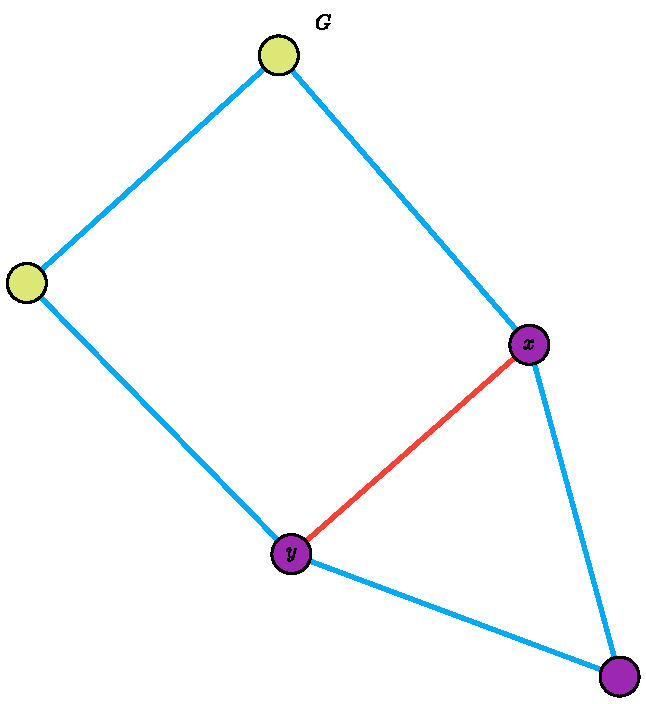
\includegraphics[width=0.5\columnwidth]{"./Editor de Grafos/Figuras/Clase 20/Dibujo 1 - Ejercicios.pdf"}
\captionof{figure}{Ilustración de una cuerda $xy$ en un grafo $G$ generado por un ciclo impar. Los vértices \purple{violeta} representan el subciclo impar $C_1$.}
\end{center}
\end{solution}

\begin{exercise}
Probar que si $G$ es un grafo $k$-crítico, entonces $\delta (G) \geq k-1$.
\end{exercise}
\begin{solution}
En efecto, si existiera $v \in G$ tal que $d (v) \leq k-2$, entonces podríamos fácilmente extender un $(k-1)$-coloreo de $G \setminus \{v\}$ a un $(k-1)$-coloreo de $G$. Sin embargo, $\chi (G) = k$. Esto prueba que $\delta (G) \geq k-1$.
\end{solution}

\begin{exercise}
Mostrar que todo grafo $k$-cromático crítico es $(k-1)$-arista-conexo.
\end{exercise}
\begin{solution}
Notar que esto equivale a que cualquier enlace (conjunto de corte minimal) tenga almenos $k-1$ aristas. Luego el siguiente lema aplicado a $X = \{v\}$ e $Y = V(G) \setminus \{v\}$, implica el resultado:
\end{solution}

\begin{lemma}
Sea $G$ un grafo con $\chi (G) > k$ y una partición de los vértices de $G$ dada por $X,Y$ tal que $G[X]$ y $G[Y]$ son $k$-coloreables, entonces el corte $E(X,Y)$ tiene almenos $k$ aristas.
\end{lemma}
\begin{proof}
Tomemos particiones $A_1, \ldots, A_k$ y $B_1, \ldots, B_k$ de los vértices de $G[X]$ y $G[Y]$ respectivamente, de manera que los conjuntos son de vértices aislados. Supongamos por el absurdo que hay a lo más $k-1$ aristas en $E(X,Y)$. Consideremos el grafo bipartito $H$ con vértices $A_i$, $B_j$ donde $A_i{B_j}$ es una arista si y solo si no existe una $A_i,B_j$-arista en $E(X,Y)$. Entonces $H$ tiene más de $k(k-1)$ aristas. Por el Ejercicio \ref{exercise:matching perfecto de un n-n bigrafo tal que hay mas de n(n-1) aristas}, esto implica que $H$ tiene un matching perfecto. Digamos que esta biyección relaciona $A_1$ con $B_1$, $A_2$ con $B_2$, etc.

Así, pintando $A_i$ y $B_i$ de color $i$ en $G$, obtenemos qune $k$-coloreo de $G$: no hay aristas entre $A_i$ y $B_i$ para todo $i =1, \ldots, k$. Esto es una contradicción, pues por hipótesis $\chi (G) > k$. Con lo cual, $E(X,Y)$ tiene almenos $k$ aristas, como queríamos demostrar.
\end{proof}




\begin{exercise}
Calcule el número cromático de un grafo en términos del número cromático de sus bloques.

\textbf{Respuesta:} $\boxed{\chi (G) = \max_{\substack{B \subset G \\ \text{$B$ bloque}}} \chi (B).}$
\end{exercise}
\begin{solution}
Afirmación: el número cromático de un grafo $G$ es $\max_B \chi (B) =:m$, donde recorremos todos los bloques $B \subset G$.

Sin pérdida de generalidad, podemos asumir que $G$ es conexo. Por un lado, como un $\chi (G)$-coloreo sirve para todo $B$, tenemos que $\max_B \chi (B) \leq \chi (G)$. Probaremos ahora la desigualdad recíproca.

Proseguiremos por inducción en la cantidad de vértices $b$ del árbol bloque de $G$. Si $b = 1$ no hay nada que probar. En general, supongamos que $b > 1$ y consideremos un bloque $B$ que corresponda a una hoja del árbol (notar que el grafo bloque nunca tiene hojas que sean vértices de corte de $G$). Consideremos $G' = G/B$, su grafo bloque tiene menos vértices pues como $b > 1$, $B$ no puede ser un solo vértice. Los grafos bloques de $G'$ son los grafos bloques de $G$ exceptuando $B$, luego por hipótesis inductiva $\chi (G') = \max_{B' \neq B} \chi (B')$.

Ahora, podemos combinar el coloreo de $B$ con el de $G'$: sea $v \in B$ el único vértice de corte de $G$ contenido en $B$ ($B$ es una hoja del grafo bloque), y denotemos con el mismo nombre al vértice de $G'$ obtenido por contraer $B$. Coloreamos $B$ con $\chi (B)$ colores y lo juntamos con un $\chi (G')$-coloreo de $G'$, simplemente permutamos los colores de $B$, de ser necesario, para que $v$ tenga el mismo color en $B$ y en $G'$. Este coloreo de $G$ usa $\max \{ \chi (B), \chi (G') \} = m$ colores. Así, $\chi (G) \leq m$, como queríamos demostrar.
\end{solution}










\subsection{Coloreo de aristas}

\begin{definition}
Llamamos \textbf{coloreo de aristas} de un grafo $G = (V,E)$ a una función $c : E \rightarrow S$ con $c(e) \neq c(f)$ si $e$ y $f$ son aristas adyacentes.

Un \textbf{$k$-arista-coloreo} de $G$ es un coloreo de ristas $c : E \rightarrow \{1,\ldots,k\}$.

El \textbf{índice cromático} de un grafo $G$, denotado por $\chi' (G)$, es el menor $k$ tal que $G$ tiene un $k$-arista-coloreo.
\end{definition}

\begin{Remark}
Si $L(G)$ es el grafo línea de $G$, entonces
\[
    \chi ' (G) = \chi (L(G)).
\]
Con lo cual, colorear aristas es un caso particular de coloreo de vértices.
\end{Remark}

\begin{obs}
Notar que siempre se tiene
\[
    \chi ' (G) \geq \Delta (G).
\]
ya que si $v \in G$ tiene grado $d_G (v) = \Delta (G)$, entonces hay $\Delta (G)$ aristas todas incidentes en $v$, i.e. no pueden tener el mismo color.

Por otro lado, sea $L(G)$ el grafo línea de $G$, tenemos que
\[
    \chi ' (G) = \chi (L (G)) \leq \Delta (L(G)) + 1 \quad \quad (\text{Proposición \ref{prop:algoritmo gloton}})
\]
y además, $\Delta (L(G)) \leq 2 \Delta (G) -2$ pues toda arista $e \in E(G)$ tiene dos vértices extremos, y por lo tanto hay $\leq 2 (\Delta (G) - 1)$ aristas incidentes en $e$: una por cada vecino de sus extremos (sin contar $e$).
\InscapeDEPRECADO{Arista $e = xy$ con a lo más $\Delta (G)- 1$ vecinos incidentes en cada extremo $x$, $y$.}
\end{obs}



\begin{theorem}[König (1916)]\label{th:todo grafo bipartito cumple que su numero cromatico es Delta}
Todo grafo bipartito $G$ cumple $\chi' (G) = \Delta (G)$.
\end{theorem}
\begin{proof}
Haremos inducción en la cantidad de aristas $\Abs G$ de $G$. Si $\Abs G = 0,1$ es trivial. Ahora, supongamos que $\Abs G \geq 1$ y que el teorema se cumple para cualquier grafo con menos aristas. Sea $\Delta := \Delta (G)$.

Tomemos una arista $xy \in \Abs{G}$ de manera que $\Delta (G -xy) = \Delta$, y un $\Delta$-arista-coloreo de $G - xy$, que existe por hipótesis inductiva. Digamos que las aristas con color $\alpha$ en nuestro coloreo de $G - xy$ son \textbf{$\alpha$-aristas}, $\alpha \in \{1, \ldots, \Delta\}$. En $G - xy$, los vértices $x$ e $y$ son incidentes en a lo más $\Delta -1$ aristas cada una.

\InscapeDEPRECADO{$\Delta$-arista-coloreo de $G -xy$ con $\Delta = 5$.}

Entonces hay colores $\alpha, \beta \in \{1,\ldots,\Delta\}$ tales que $x $ no es adyacente aninguna arista de color $\alpha$ e $y$ no es adyacente a ninguna arista de color $\beta$. Si $\alpha = \beta$, entonces puedo extender el coloreo de $G-xy$ a un coloreo de $G$ asignando a $xy$ el color $\alpha$. Consecuentemente, podemos asumir que $\alpha \neq \beta$ y que $x$ incide en una arista de color $\beta$.

Ahora, consideremos la sucesión de aristas $e_1, \ldots, e_r$ de longitud máxima $r$, que empieza con la arista de color $\beta$ incidente en $x$ y va alternando colores de la siguiente manera: $e_1$ tiene color $\beta$, $e_2$ color $\alpha$, etc... Notemos que ninguna arista de color $\alpha$ cubre a $y$, pues si denotamos por $X,Y$ a la bipartición de los vértices de $G$, con $x \in X, y \in Y$, entonces un extremo en $Y$ de una arista de color $\alpha$ siempre tiene una arista de color $\beta$ incidente y por lo tanto no puede ser $y$ (se puede probar fácilmente por inducción en $r$). Luego, intercambiando los colores de esta sucesión de aristas\footnote{Observar que la sucesión que construimos es una componente de una cadena de Kempen $H_{\alpha, \beta}$ en el grafo de línea $L(G)$.}, obtenemos un arista coloreo tal que $x,y$ no tienen aristas incidentes de color $\beta$, luego extendemos este coloreo a $G$ pintando $xy$ de color $\beta$.
\end{proof}



\begin{theorem}[Vizing (1964)]
Todo grafo $G$ cumple
\[
    \boxed{\Delta (G) \leq \chi ' (G) \leq \Delta (G) +1 .}
\]
\end{theorem}







%%%%%%%%%%%
\Clase{16/06/23}   %%%%%%%%%%%%%%%%%%%%%%%%%%%%%%%%%%%%%%%%%%%%%%%%%%%%%%%%%%%%%
%%%%%%%%%%%


\subsection{Lista coloreo}

\begin{definition}
Sea $(S_v)_{v \in G}$ una familia de conjuntos de colores. Si un coloreo $c$ de $V(G)$ es tal que $c(v) \in S_v$ para todo $v \in V(G)$, entonces decimos que $c$ es un \textbf{coloreo de las listas $S_v$}.

Un grafo es \textbf{k-lista-coloreable}, si para cada familia $(S_v)_{v \in G}$ con $\abs {S_v} = k$ hay un coloreo de las listas $S_v$.

El \textbf{número lista-cromático}, denotado por $\ch G$, de un grafo $G$ es el menor $k$ tal que $G$ es $k$-lista-coloreable.
\end{definition}

\begin{example}\label{ejemplo:ejemplo de grafos bipartitos que no son k-lista coloreables}
El grafo $K_{2,4}$ no es $2$-lista-coloreable, para eso, basta ver que existe una familia de listas de tamaño $2$ que no colorea. Consideremos:

\InscapeDEPRECADO{Coloreo de una elección de listas de tamaño $2$ que es imposible de que funcione.}

Es fácil extender esta idea para cualquier cantidad $k$, utilizando grafos bipartitos completos $K_{k, k^k}$. En efecto, si particionamos $K_{k,k^k}$ en $\{u_i\}_{i = 1}^k$ y $\{w_j\}_{j = 1}^{k^k}$, luego no podemos usar la siguiente lista para $k$-colorear: $S_{u_i} = \{(i-1)k + 1, \ldots, ik\}$, y $S_{w_j}$ son todas las maneras de construir un conjunto de $k$ elementos eligiendo uno de cada $S_{u_i}, \: \: i = 1 , \ldots, k$. Es claro que no podemos colorear con estas listas, pues dado un coloreo $c(u_i) \in S_{u_i}$ siempre podemos encontrar, por construcción, un vérticce $w_j$ adyacente a todos los $u_i$, tal que $S_{w_j} = \{ c(u_i) | i = 1, \ldots, k\}$.
\end{example}


\begin{proposition}\label{proposicion:choice es menor o igual que coloreo menor o igual que delta + 1}
\begin{enumerate}
\item Tenemos que $\ch G \leq \col G$. En particular
\[\ch G \leq \Delta (G) + 1.\]
\item Hay una versión de Brooks para $\ch G$: si $G$ no es completo ni ciclo impar, entonces $\ch G \leq \Delta (G)$.
\end{enumerate}
\end{proposition}
\begin{proof}
Solo probaremos la primera afirmación, pues la segunda es más dificil.

Sea $\{v_i\}_{i = 1}^n$ un ordenamiento arbitrario de los vértices de $G$, y sea
\[
    d = \max_{i>1}d_{G[v_1, \ldots, v_{i-1}]} (v_i) + 1.
\]
Entonces $G$ es $d$-lista-coloreable: aplicamos el algorítmo glotón en este orden. Luego $\ch G \leq d$. Como el orden era arbitrario, tomando un orden que minimice $d$, se sigue que $\ch G \leq \col G$.
\end{proof}




\bigskip

Similarmente, podemos estudiar coloreo de aristas por listas:

\begin{definition}
Sea $(S_e)_{e \in E(G)}$ una familia de conjuntos de colores. Si un coloreo $c$ de $E(G)$ es tal que $c(e) \in S_e$ para todo $e \in E(G)$, entonces decimos que $c$ es un \textbf{coloreo de las listas $S_e$}, donde se entiende por contexto que estamos coloreando aristas.

Un grafo es \textbf{k-arista-lista-coloreable}, si para cada familia $(S_e)_{e \in E(G)}$ con $\abs {S_e} = k$ hay un coloreo de las listas $S_e$.

El \textbf{índice lista-cromático}, denotado por $\operatorname{ch}' (G)$, de un grafo $G$ es el menor $k$ tal que $G$ es $k$-arista-lista-coloreable.
\end{definition}

\begin{Obs}
El coloreo de aristas por listas de un grafo $G$ es equivalente a colorear por listas los vértices del grafo línea $L(G)$. En particular, $\operatorname{ch}' (G) = \ch {L(G)}$
\end{Obs}

A priori, probar que un grafo es $k$-lista-coloreable (o $k$-arista-lista-coloreable) es más difícil que probar que es $k$-coloreable ($k$-arista-coloreable): este último es un caso particular de coloreo por las listas $S_v = \{1,\ldots, k\}$ para todo $v \in G$ ($S_e = \{1, \ldots, k\}$ para todo $e \in E(G)$). Por lo tanto,
\[
    \ch G \geq \chi (G) \quad (\operatorname{ch}' (G) \geq \chi ' (G))
\]
para cualquier grafo $G$.

Estas desigualdades en muchos casos \textit{no son óptimas}: el Ejemplo \ref{ejemplo:ejemplo de grafos bipartitos que no son k-lista coloreables} muestra que para todo $k \geq 1$, existe un grafo bipartito (y por lo tanto $2$-coloreable) que no es $k$-lista coloreable.

Al contrario del caso vértices, \underline{se desconoce actualmente} si existen grafos tal que $\operatorname{ch}' (G) > \chi ' (G)$. De hecho, se conjetura:
\begin{conjecture}
\[
    \operatorname{ch}' (G) = \chi ' (G).
\]
\end{conjecture}
Veamos que la conjetura vale para el caso particular de grafos bipartitos.

Para eso, recordemos que si $D$ es un grafo dirigido y $v \in V(D)$, denotamos por $N^+ (v)$ al conjunto de vecinos, y por $d^+ (v)$ al número de vecinos, $w \in D$ tales que $D$ contiene una arista dirigida desde $v$ hasta $w$.

\begin{definition}
Sea $D$ un grafo dirigido. Llamamos a un conjunto independiente de vértices $U \subset V(D)$ un \textbf{núcleo} de $D$, si para todo vértice de $v \in D \setminus U$, existe una arista dirigida en $D$ desde $v$ hacia un vértice de $U$.
\end{definition}
Notar que los núcleos de un grafo dirigido $D$ no vacío son no vacíos también.

\begin{lemma}[Lema del Núcleo]\label{lema:lema del nucleo}
Sea $H$ un grafo y $(S_v)_{v \in H}$ una familia de listas. Si $H$ tiene una orientación $D$ con $d^+ (v) < \abs{S_v}$ para todo $v$, tal que todo subgrafo inducido de $D$ tiene un núcleo, entonces $H$ puede ser coloreado a partir de las listas $S_v$.
\end{lemma}
\begin{proof}
Haremos inducción en $n = \abs{H}$. Si $n = 0$ simplemente tomamos el \textit{coloreo vacío}. Para el paso inductivo, supongamos que $n > 0$. Sea $\alpha$ un color de alguna de las listas $S_v$, y sea $D$ una orientación de $H$ dada por el enunciado. Los vértices $v$ con $\alpha \in S_v$ generan un subgrafo (inducido) no vacío $D'$ de $D$, el cual por hipótesis tiene un núcleo $U \neq \emptyset$.

Coloreemos los vértices de $U$ con $\alpha$, y removamos $\alpha$ de las listas de todos los vértices de $D' \setminus U$. Como cada uno de estos vértices manda una arista hacia $U$, las listas modificadas $S'_v, \: \: v \in D \setminus U$ siguen cumpliendo la condición $d^+_{D \setminus U} (v) < \abs{S'_v}$ en $D \setminus U$. Como $D \setminus U$ es una orientación de $H \setminus U$, podemos colorear $H \setminus U$ a partir de estas listas por hipótesis inductiva. Como ninguna de estas listas contiene a $\alpha$, podemos extender este coloreo a $U$, coloreando los vértices de $U$ con $\alpha$. Así obtenemos el coloreo deseado de $H$.
\end{proof}

\begin{theorem}[Galvin (1995)]
Todo grafo bipartito tiene $\operatorname{ch}' (G) = \chi ' (G)$.
\end{theorem}
\begin{proof}
Sea $G$ un $X,Y$-bigrafo con conjunto de aristas $E$. Diremos que dos aristas de $G$ \textbf{se reunen en} $X$, si comparten un mismo extremo en $X$ (Análogamente podemos definir qué significa que dos aristas se reunan en $Y$). Sea $\chi ' (G) = k$, y sea $c$ un $k$-coloreo de las aristas de $G$.

Ya hemos visto que $\operatorname{ch}' (G) \geq k$; luego basta probar la otra desigualdad: $\ch G ' \leq k$. El plan es aplicar el lema anterior al grafo linea $H:= L(G)$ de $G$ para probar que es $k$-lista coloreable. Para eso, basta encontrar una orientación $D$ de $H$ con $d^+ (e) < k$ para todo vértice $e \in H$, de tal suerte que para cada subgrafo inducido $D$ existe un núcleo. Para definir $D$, consideremos dos aristas adyacentes $e, e' \in E$, digamos con color $c(e) < c(e')$. Si $e$ y $e'$ se reunen en $X$, orientamos la arista $ee' \in H$ desde $e'$ hacia $e$; si $e$ y $e'$ se reunen en $Y$, orientamos $e$ hacia $e'$.

\InscapeDEPRECADO{Orientación del grafo línea $H$ de $G$.}

Calculemos $d^e (e)$ para cualquier $ e \in V(D)$. Si $c(e) = i$, luego todo $e' \in N^+_D (e)$ que se reune en $X$ con $e$, tiene color en $\{1, \ldots, i-1\}$, y si se reune en $Y$ con $e$, tiene color en $\{i+1, ldots, k\}$. Además, dados dos vecinos de $e$ que se reunen en el mismo conjunto $X$ o $Y$ deben tener distinto color, con lo cual $d^+_D (e < k)$.

Falta ver que todo subgrafo inducido $D'$ de $D$ tiene núcleo. Esto es un corolario inmediato del Teorema del Matrimonio \ref{th:teorema del matrimonio estable} para $G$, si interpretamos las direcciones en $D$ como expresando preferencia. En efecto, dado un vértice $v \in X \cup Y$ y aristas $e, e' \in V(D')$ indidentes a $v$, escribimos $e <_v e'$ sii la arista $ee'$ de $H$ es dirigida de $e$ en $e'$ in $D$. Así, todo matching estable en el grafo bipartito $(X \cup Y, V(D'))$ para esta preferencia es un núcleo en $D'$. (¿Cuál es un matching estable en la figura anterior?)
\end{proof}

\begin{corollary}
Todo grafo bipartito $G$ satisface:
\[
    \boxed{\operatorname{ch}' (G) = \Delta (G).}
\]
\end{corollary}
\begin{proof}
Por el teorema, tenemos que $\operatorname{ch}' (G) = \chi ' (G)$. Por otro lado, $\chi ' (G) = \Delta (G)$ por el Teorema \ref{th:todo grafo bipartito cumple que su numero cromatico es Delta}.
\end{proof}



\subsection{Grafos perfectos}

\begin{definition}
El mayor número entero $n$ tal que $K_n \subset G$ como subgrafo, es el \textbf{número de clique} $\omega (G)$ de $G$.
\end{definition}
Claramente $\omega (G) \leq \chi (G)$, puesto que $\chi (K_m) = m$ para todo $m \geq 1$.

\begin{obs}
Sea $\alpha (G)$ el máximo número de vértices independientes de $G$. Observar que tenemos la siguiente dualidad: $\alpha (G) = \omega (\bar G)$ y que $\omega (G) = \alpha (\bar G)$.
\end{obs}

\begin{definition}
Llamamos a un grafo \textbf{perfecto}, si para todo subgrafo inducido $H \subset G$ tiene número cromático $\chi (H) = \omega (H)$.
\end{definition}
En otras palabras, la cota obvia $\omega (H) \leq \chi (H)$ siempre basta para colorear $H$. Así, para probar que $\chi (G) > k$ en un grafo perfecto $G$, equivale a encontrar un subgrafo $K_{k+1}$ de $G$, que \textit{certifique} la no $k$-coloreabilidad de $G$.

\begin{remark}
Parecería que la clase de grafos perfectos fue definida de manera ``artificiar'': a pesar de ser cerrado bajo subgrafos inducidos (por definición), no es cerrado en general para subgrafos o supergrafos, mucho menos menores. Sin embargo, el concepto de perfección es sumamente importante para la teoría de grafos, pues existen varias clases fundamentales de grafos que son también perfecto; más aún, esta clase de grafos posee propiedades de dualidad con profundas conexiones con teoría de optimización y complejidad.
\end{remark}

\bigskip

Existen varios ejemplos de tipos de grafos perfectos. Algunos serán mencionados en los ejercicios. Ahora, veremos que un tipo de grafo es perfecto: loso grafos \textit{cordales}:

\begin{definition}
Decimos que un grafo es \textbf{cordal} (o \textbf{triangulado}) si cada uno de sus ciclos de longitud $\geq 4$ tiene una cuerda, es decir, sus únicos subciclos inducidos son triángulos.
\end{definition}

Antes de seguir, si $G$ posee subgrafos inducidos $G_1,G_2$ y $S$, tales que $G = G_1 \cup G_2$ y $S = G_1 \cap G_2$, diremos que $G$ se obtiene a partir de $G_1$ y $G_2$ \textbf{pegando} estos grafos a lo largo de $S$.

\begin{proposition}
Un grafo es cordal si y solo si puede construirse recursivamente pegando grafos completos a lo largo de subgrafos completos.
\end{proposition}
\begin{proof}
Si $G$ sse obtiene a partir de dos grafos cordales $G_1,G_2$ pegando ambos a lo largo de un subgrafo completo, entonces $G$ es claramente cordal: cualquier subciclo inducido de $G$ yace en $G_1$ o $G_2$, y es por lo tanto un triangulo. Como los grafos completos son cordales, esto prueba que todos los grafos construidos de esta manera son cordales.

Recíprocamente, sea $G$ un grafo cordal. Probaremos por inducción en $n = \abs G$ que podemos construir $G$ de esta manera. Esto es trivial si $G$ es completo. Con lo cual, supongamos que $G$ no es completo, en particular $n > 1$. Sean $a,b \in G$ dos vértices no adyacentes, y sea $X \subset V(G) \setminus \{a,b\}$ un conjunto minimal que separa $a$ y $b$. Sea $C$ la componente de $G \setminus X$ que contiene $a$, y escribamos $G_1 := G[V(C) \cup X]$ y $G_2 := G \setminus C$. Entonces $G$ se obtiene a partir de $G_1$ y $G_2$ al pegar estos grafos a lo largo de $S:= G[X]$.

Como $G_1$ y $G_2$ son ambos cordales (al ser subgrafos inducidos de $G$), se construyen por inducción de esta manera, con lo cual, basta ver que $S$ es completo. Por el absurdo, supongamos que existen $s,t \in S$ que no son adyacentes. Por la minimalidad de $X = V(S)$ como separador de $a,b$, tenemos que ambos $s$ y $t$ tienen un vecino en $C$. Por lo tanto, existe un $X$-camino de $s$ en $t$ en $G_1$; sea $P_1$ uno de estos caminos de tamaño mínimo. Análogamente, $G_2$ contiene un $X$-camino de tamaño mínimo, digamos $P_2$, desde $s$ hasta $t$. Entonces $P_1 \cup P_2$ es un ciclo sin cuerdas de longitud $\geq 4$, absurdo: $G$ es cordal.

\InscapeDEPRECADO{Si $G_1$ y $G_2$ son cordales, entonces $G$ también.}
\end{proof}


\begin{proposition}
Todo grafo cordal es perfecto.
\end{proposition}
\begin{proof}
Como los grafos completos son perfectos, por la proposición anterior basta probar que todo grafo $G$ obtenido a partir de dos grafos perfectos $G_1,G_2$ luego de pegarlos a lo largo de un subgrafo completo $S$ es nuevamente perfecto. Luego seae $H \subset G$ cualquier subgrafo inducido; veamos que $\chi (H) \leq \omega (H)$.

Sea $H_i := H \cap G_i$ para $i =1,2$ y sea $T := H \cap S$. Entonces $T$ es nuevamente completo, y $H$ se obtiene a partir de $H_1,H_2$ pegando a lo largo de $T$. Cada $H_i$ es un subgrafo inducido de $G_i$, y se puede colorear por $\omega (H_i)$ colores. Como $T$ es completo, ambos coloreos $H_1$ y $H_2$ se pueden combinar, luego de permutar los colores de alguno de ellos, tal que obtenemos un coloreo de $H$ con $\max \{\omega (H_1), \omega(H_2) \} \leq \omega (H)$ colores.
\end{proof}

Una caracterización muy famosa de los grafos perfectos vía una familia de subgrafos inducidos prohibidos: Los ciclos impares de grado $\geq 5$ y sus complementos.

\begin{theorem}[El Teorema Fuerte de Grafos Perfectos - Chudnovsky, Robertson, Symour \& Thomas (2006)]
Un grafo $G$ es perfecto si y solo si $G$ ni $\bar G$ contienen un ciclo impar de longitud $\geq 5$ como subgrafo inducido.
\end{theorem}

La demostración de este resultado es muy largo y complicado, sin embargo, probaremos de manera elemental dos corolarios inmediatos de este teorema:

\begin{theorem}[Lovász (1972)]\label{th: lovasz 1 - todo grafo es perfecto si y solo si su complemento lo es}
Un grafo es perfecto si y solo si su complemento lo es.
\end{theorem}

\begin{theorem}[Lovász (1972)]
Un grafo $G$ es perfecto si y solo si
\[
    \abs H \leq \alpha (H) \cdot \omega (H)
\]
para todo subgrafo inducido $H \subset G$.
\end{theorem}

Antes de probar ambos resultados, necesitamos un lema. Sea $G$ un grafo y $x \in G$ un vértice, sea $G'$ obtenido a partir de $G$ al agregar un vértice $x'$ y uniéndolo a $x$ y a todos los vecinos de $x$. Decimos que $G'$ se obtiene a partir de $G$ al \textbf{expandir} el vértice $x$ a una arista $xx'$.

\InscapeDEPRECADO{Expansión de un vértice $x$ en la demostración del Lema \ref{lema:la expansion de un grafo perfecto es perfecto}.}

\begin{lemma}\label{lema:la expansion de un grafo perfecto es perfecto}
Todo grafo obtenido a partir de un grafo perfecto al expandir un vértice es nuevamente perfecto.
\end{lemma}
\begin{proof}
Sea $G$ un grafo perfecto, haremos inducción en $n = \abs G$. Expandir el vértice de $K_1$ nos da $K_2$, el cual es perfecto, esto prueba $n = 1$. En general, sea $n >1$ y $G'$ el grafo obtenido a partir de $G$ luego de expandir un vértice $x \in G$ a una arista $xx'$. Para probar que $G'$ es perfecto, basta ver que $\chi (G') \leq \omega (G')$. En efecto todo subgrafo propio inducido $H$ de $G'$ es isomorfo a un subgrafo inducido de $G$ o se obtiene a partir de un subgrafo propio inducido de $G$ al expandir $x$; en cualquier caso, $H$ es perfecto por hipótesis inductiva, y por loi tanto puede ser coloreado por $\omega (H) $ colores.

Sea $\omega := \omega (G)$, entonces $\omega (G') = \omega$ o $\omega + 1$. Si $\omega (G') = \omega + 1$, entonces
\[
    \chi (G') \leq \chi (G) + 1 = \omega + 1 = \omega (G')
\]
y ganamos. Supongamos entonces que $\omega (G') = \omega$. Luego $x$ no yace en ningún subgrafo de $G$ isomorfo a $K_\omega$: de lo contrario, junto con $x'$ formaría un $K_{\omega + 1}$ de $G'$ y por lo tanto $\omega (G')$ sería $\omega + 1$, absurdo. Luego pintemos $G$ con $\omega$ colores. Como todo $K_\omega \subset G$ contiene un vértice del mismo color que $x$ (llamemos $X$ al conjunto de vértices de $G$ con el mismo color de $x$), pero no a $x$, el grafo $H:= G \setminus (X \setminus \{x\})$ tiene número de clique $\omega (H) < \omega$ (ver la figura anterior \ref{Figura:Clase \thenumeroClase - Dibujo \thenumeroDibujo}). Como $G$ es perfecto, podemos colorear $H$ con $\omega -1$ colores. Ahora, $X$ es un conjunto independiente, con lo cual el conjunto $(X \setminus \{x\}) \cup  \{x'\} = V(G' - H)$ es también independiente. Así, podemos extender el $(\omega -1)$-coloreo de $H$ a un $\omega$-coloreo de $G'$. Consecuentemente, $\chi (G') \leq \omega = \omega (G')$, como queríamos probar.
\end{proof}

Probemos ahora los dos teoremas.

\begin{theorem}[Lovász (1972)]
Un grafo es perfecto si y solo si su complemento lo es.
\end{theorem}
\begin{proof}
Como $\bar {\bar G} = G$, basta ver que si $G = (V,E)$ es perfecto, entonces su complemento también. Hagamos inducción en $n = \abs G$.
Si $n = 1$ esto es trivial, luego en general supongamos que $n \geq 2 $. Sea $\Kappa := \{V(K) | K \subset G \text{ es un subgrafo completo} \}$. Escribamos $\alpha := \alpha (G)$, y sea $\mathcal A := \{U \subset G | \text{$U$ es un conjunto independiente de vértices, con $\abs U = \alpha$}\}$.

Todo subgrafo propio inducido de $\bar G$ es el complemento de un subgrafo propio inducido de $G$, y por lo tanto es perfecto por inducción. Con lo cual, para ver que $\bar G$ es perfecto, basta ver que $\chi (\bar G) \leq \omega (\bar G) = \alpha$. Para esto, encontraremos $K \in \Kappa$ tal que $K \cap A \neq \emptyset$ para todo $A \in \mathcal A$; consecuentemente
\[
    \omega (\bar G \setminus K ) = \alpha (G \setminus K) < \alpha = \omega (\bar G),
\]
luego por hipótesis inductiva:
\[
    \chi (\bar G) \overset{\text{$K$ es independiente en $\bar G$}}{\leq} \chi (\bar G \setminus K )+ 1 = \omega (\bar G \setminus K) + 1 \leq \omega (\bar G)
\]
como queríamos.

Ahora, veamos que existe $K$ cumpliendo lo deseado. Para eso, supongamos por el absurdo que no, es decir, para todo $K \in \Kappa$ existe un $A_K \in \mathcal A$ tal que $K \cap A_K = \emptyset$. Reemplacemos en $G$ a cada vértice $x$ por un grafo completo $G_x$ de orden
\[
    k(x) := \abs{\Set{K \in \Kappa | x \in A_K}},
\]
y uniendo todos los vértices de $G_x$ con todos los vértices de $G_y$ si $xy \in E$. Así, obtenemos un grafo $G'$. Más aún, $G'$ se puede obtener al aplicar repetidas veces una expansión de vértices del grafo $G[\set{x \in V | k(x) > 0}]$. Al ser este un subgrafo inducido de $G$, debe ser perfecto, y por el Lema \ref{lema:la expansion de un grafo perfecto es perfecto}, $G'$ es perfecto. En particular,
\begin{equation}\label{eq:clase 21 - coloreo - Teorema 1- eq 1}
\chi (G') \leq \omega (G').
\end{equation}

Para obtener una contradicción a \eqref{eq:clase 21 - coloreo - Teorema 1- eq 1}, calcularemos los valores de $\omega (G')$ y de $\chi (G')$. Por construcción de $G'$, todo subgrafo maximal completo de $G'$ es de la forma $G'[\bigcup_{x \in X} G_x]$ para algún $X \in \Kappa$. Con lo cual, existe un $X \in \Kappa$ tal que
\begin{align}
\omega (G') &= \sum_{x \in X} k(x) \nonumber \\
            &= \abs{\Set{(x, K) |  x\in X, K \in \Kappa, x \in A_K}} \nonumber \\
            &= \sum_{K \in \Kappa} \abs{X \cap A_K} \nonumber \\
            &\leq \abs{\Kappa} -1 , \label{eq:clase 21 - coloreo - Teorema 1- eq 2}
\end{align}
donde la última desigualdad se sigue de que $\abs {X \cap A_K} \leq 1$ para todo $K$, ya que $A_K$ es independiente pero $G[X]$ es completo, además $\abs{X \cap A_X} = 0$ por como elegimos $A_X$.

Por otro lado,
\begin{align*}
\abs{G'} &= \sum_{x \in V} k(x) \\
        &= \abs{\Set{(x, K) | x \in V, K \in \Kappa, x \in A_K}} \\
        &= \sum_{K \in \Kappa} \abs{A_K} \\
        &= \abs{\Kappa} \cdot \alpha.
\end{align*}
Como $\alpha (G') \leq \alpha$ por construcción de $G'$, tenemos que

\begin{equation}\label{eq:clase 21 - coloreo - Teorema 1- eq 3}
\chi (G') = \omega (G') = \sum_{K \in \Kappa}  \frac{\abs{G'}}{\alpha (G')} \geq \frac{\abs {G'}}{\alpha} = \abs{\Kappa},
\end{equation}
donde la primera desigualdad vale para todo grafo: las clases de colores de $G'$ particionan a $G'$ en conjuntos independientes (y por lo tanto tienen cardinal $\leq \alpha (G')$).

Juntando \eqref{eq:clase 21 - coloreo - Teorema 1- eq 2} y \eqref{eq:clase 21 - coloreo - Teorema 1- eq 3}, obtenemos
\[
    \chi (G') \geq \abs{\Kappa} > \abs{\Kappa} - 1 \geq \omega (G'),
\]
contradiciendo \eqref{eq:clase 21 - coloreo - Teorema 1- eq 1}.
\end{proof}

\begin{obs}\label{obs:bipartitos son perfectos}
Claramente los grafos bipartitos son perfectos. Luego, el teorema anterior implica que el complemento de un grafo bipartito también es perfecto.
\end{obs}

\begin{theorem}[Lovász (1972)]
Un grafo $G$ es perfecto si y solo si
\[
    \abs H \leq \alpha (H) \cdot \omega (H)
\]
para todo subgrafo inducido $H \subset G$.
\end{theorem}
\begin{proof}
Escribamos $\{v_1, \ldots,v_n\} := V(G)$, $\alpha := \alpha (G)$ y $\omega = \omega (G)$. La necesidad es inmediata: si $G$ es perfecto, entonces todo subgrafo inducido $H$ de $G$ puede ser particionado en a lo más $\omega (H)$ clases de colores, cada una conteniendo a lo más $\alpha (H)$ vértices.

Para probar la recíproca, haremos inducción en $n = \abs G$. Supongamos que cada subgrafo inducido $H$ de $G$ cumple la desigualdad $\abs H \leq \alpha (H) \cdot \omega (H)$, pero que $G$ no es perfecto. Por hipótesis inductiva, todo subgrafo inducido propio de $G$ es perfeccto. Con lo cual, todo subconjunto independiente no vacío $U \subset V(G)$ satisface:
\begin{equation}\label{eq:clase 21 - coloreo - Teorema 2- eq 1}
\chi (G \setminus U) = \omega (G \setminus U) = \omega,
\end{equation}
en efecto, la primera igualdad proviene de la perfección de $G \setminus U$, mientras que $\omega (G \setminus U) \leq \omega$ es obvia, y además si $\chi (G \setminus U) < \omega$, luego tendríamos que $\chi (G) \leq \omega$, y por lo tanto $G$ sería perfecto, contradiciendo nuestra suposición.

Así, apliquemos \eqref{eq:clase 21 - coloreo - Teorema 2- eq 1} al singleton $U = \{u \}$ y consideremos un $\omega$-coloreo de $G \setminus \{u\}$. Sea $K$ el conjunto de vértices de algún $K_\omega$ en $G$. Claramente,
\begin{enumerate}[(1)]
\item si $u \not \in K$, entonces $K$ contiene un color de cada clase de $G \setminus \{u\}$;
\item Si $u \in K$, entonces $K$ contiene un color de todas las clases, salvo exactamente una, de $G \setminus \{u\}$.
\end{enumerate}

Sea $A_0 = \{u_1, \ldots, u_\alpha\}$ un conjunto independiente de $G$ de tamaño $\alpha$. Sean $A_1, \ldots, A_\omega$ las clases de colores de un $\omega$-coloreo de $G \setminus \{u_1\}$, y sean $A_{\omega + 1}, \ldots, A_{2\omega}$ las clases de colores de un $\omega$-coloreo de $G \setminus \{u_2\}$, y así sucesivamente. En total, obtenemos $\alpha \omega + 1$ conjuntos independientes $A_0, A_1, \ldots, A_{\alpha \omega}$ en $G$. Para cada $i = 0, \ldots, \alpha \omega$, existe por \eqref{eq:clase 21 - coloreo - Teorema 2- eq 1} un subgrafo completo $K_\omega \subset G \setminus A_{i}$; denotemos por $K_i$ al conjunto de sus vértices.

Notar que si $K'$ es un conjunto de vértices de cualquier subgrafo completo $K_\omega$ de $G$, entonces
\begin{equation}\label{eq:clase 21 - coloreo - Teorema 2- eq 2}
K' \cap A_i = \emptyset \text{ para exactamente un $i = 0 , \ldots, \alpha \omega$}.
\end{equation}
En efecto, si $K' \cap A_0 = \emptyset$, entonces $K' \cap A_i \neq \emptyset$ para todo $i > 0$, por definición de $A_i$ y por el ítem (1). Similarmente, si $K' \cap A_0 \neq \emptyset$, entonces $\abs{K' \cap A_0} = 1$, con lo cual $K \cap A_i = \emptyset$ para exactamente un $i \neq 0$: por el ítem (2) aplicado al único $u' \in K' \cap A_0$, y por el ítem (3) aplicado al resto de los vértices de $A_0 \setminus \{u'\}$.

Sea $J \in \reals^{(\alpha \omega + 1) \times (\alpha \omega + 1)}$ la matriz real con entradas cero en la diagonal principal y unos en el resto. Sea $A = (a_{ij}) \in \reals^{(\alpha \omega + 1) \times n}$ la matriz real cuyas filas son los vectores de incidencia de los conjuntos $A_i$ con $V(G)$:
\[
    a_{ij} = \begin{cases}
            1 & \text{ si $v_j \in A_i$} \\
            0 & \text{ si no}.
    \end{cases}
\]
Similarmente, sea $B \in \reals^{n \times (\alpha \omega + 1)}$ la matriz cuyas columnas son los vectores de incidencia de los conjuntos $K_j$ con $V(G)$. Ahora, como $\abs{ A_i \cap K_i} = 0$ para todo $i$ por como elegimos $K_i$, tenemos que $A_i \cap K_j \neq \emptyset$ y por lo tanto, $\abs{ A_i \cap K_j} = 1$ para todo $i \neq j$, por \eqref{eq:clase 21 - coloreo - Teorema 2- eq 2}. Consecuentemente,
\[
    AB = J.
\]
Como $J$ es no singular, tenemos que $A$ tiene rango $\alpha \omega + 1$. En particular, $n \geq \alpha \omega + 1$, contradiciendo la condición del teorema para $H = G$.
\end{proof}

%%%%%%%%%%%
\Clase{23/06/23}   %%%%%%%%%%%%%%%%%%%%%%%%%%%%%%%%%%%%%%%%%%%%%%%%%%%%%%%%%%%%%
%%%%%%%%%%%


Antes de demostrar el Teorema de Vizing \ref{th:teorema de Vizing}, necesitamos un poco de notación:
\begin{definition}
Sea $G$ un grafo con un coloreo de aristas $c: E(G) \rightarrow S$.

Dado un vértice $x \in G$, denotamos por $M(x)$ al conjunto de colores (respecto de $c$) que no aparecen en
\[
    \{c(e) | \text{$e$ incidente a $x$}\}.
\]

Decimos que $\alpha \in S$ es \textbf{faltante en $x$} (respecto de $c$) si $\alpha \in M(x)$.
\end{definition}

\InscapeDEPRECADO{Ejemplo, $c$ es un coloreo de las aristas tal que $M(x) = \{4\}$. En esta terminología, el color $4$ es \textit{faltante} en $x$.}

\begin{definition}
Nuevamente, sea $G$ un grafo con un coloreo de aristas $c: E(G) \rightarrow S$.

Si $\alpha, \beta \in S$ son dos colores distintos de $c$, llamamos \textbf{$\alpha/\beta$-camino desde $x$}, al único camino maximal que comienza en $x$ con su primer arista de color $\alpha$, su siguiente de color $\beta$ y así intercaladamente; la longitud puede ser $0$.
\end{definition}

\InscapeDEPRECADO{$\blue{\alpha}/\red{\beta}$-camino de un arista-coloreo de un grafo $G$.}

\begin{theorem}[Vizing (1964)]\label{th:teorema de Vizing}
Todo grafo $G$ cumple
\[
    \boxed{\Delta (G) \leq \chi ' (G) \leq \Delta (G) +1 .}
\]
\end{theorem}

\begin{proof}
Sea $G$ un contraejemplo arista-minimal del teorema. Notemos $\Delta = \Delta (G)$. Entonces, $E(G) \neq \emptyset$. Podemos asumir lo siguiente:

\begin{quote}
\begin{enumerate}
\item[({$\ast$})]\label{vizing-proof-condition} Sea $xy \in E(G)$ y $c$ un $(\Delta + 1)$-arista-coloreo arbitrario de $G - xy$ y $\alpha$ faltante en $x$ y $\beta$ faltante en $y$ respecto de $c$. Entonces el $\alpha/\beta$-camino desde $y$ termina en $x$.
\end{enumerate}
\end{quote}
En efecto, si no fuera cierto, podríamos intercambiar los colores $\alpha$ y $\beta$ del $\alpha/\beta$-camino y extender el coloreo $c$ a un coloreo de $G$ vía $c'(xy):= \alpha$.

Sea $uv \in E(G)$, por minimalidad $G -uv$ admite una $(\Delta +1)$-arista-coloración, digamos $c_0: E(G) \rightarrow \{1, \ldots, \Delta + 1\}$.

\InscapeDEPRECADO{}

Como $d(x) < \Delta + 1$, entonces $M(x) \neq \emptyset$ para todo $x \in V(G)$. Si $M(u) \cap M(v) \neq \emptyset$, entonces $c_0$ puede extenderse a un $(\Delta + 1)$-arista-coloreo de $G$: coloreando $uv$ con un color en $M(u) \cap M(v)$. Con lo cual, podemos suponer que $M(u) \cap M(v) = \emptyset$.

Sea $i_1 \in M(v)$. Como $M(u) \cap M(v)  = \emptyset$, existe $v_1 \in N(u)$ tal que $c_0(uv_1) = i_1$. Sea $i_2 \in M(v_1)$. Si $i_2 \in M(u)$, podemos obtener una $(\Delta+1)$-coloración de $G$, coloreando con $i_2$ a $uv_1$ y dando el color $i_1$ a la arista $uv$. Luego $u$ tiene un vecino $v_2$ con $c_0(uv_2) = i_2$ como antes, tomamos $i_3 \in M(v_2)$. Así, obtenemos una secuencia maximal $v = v_0, v_1, \ldots, v_k$ de vecinos de $u$ tales que $c_0 (uv_i) \in M(v_{i-1})$ respecto de $c_0$ para todo $0 < i \leq k$.

Luego, para cada $i = 1, \ldots, k$ definimos un coloreo $c_i$:
\begin{enumerate}[(i)]
\item $c_i (uv_j) = c_0 (u v_{j+1})$ para todo $0 \leq j < i$,
\item $c_i (uv_i)$ no está definido,
\item $c_i (e) = c_0 (e)$ para el resto de las aristas.
\end{enumerate}
Estos son $(\Delta + 1)$-arista-coloreos de $G-uv_i$. Además, notemos que los colores faltantes $M(u)$ de $u$ son los mismos para todo $c_i, \: \: 0 \leq i \leq k$.

\InscapeDEPRECADO{}

Sea $\beta \in M(v_k)$ respecto de $c_0$, entonces $\beta$ también es faltante en $v_k$ respecto de $c_i$ para todo $0 \leq i \leq k$. Notar que por \hyperref[vizing-proof-condition]{({$\ast$})} aplicado a $c = c_k$, $\beta$ no es faltante en $u$ para $c_k$. Con lo cual, $\beta \not \in M(u)$ para todo $c_i$ con $0 \leq i \leq k$. Por la maximalidad la secuencia $v_0, \ldots,v_k$, existe un $1\leq i < k$ tal que $c_0(xv_i) = \beta$. Por como definimos $c_1, \ldots, c_k$ tenemos que:
\[
    c_0 (uv_i) = c_{i-1} (uv_i) = c_k (u v_{i-1}) = \beta.
\]

Sea $\alpha \in M(u)$. Sea $P$ el $\alpha/\beta$-camino desde $v_k$ respecto de $c_k$. Por \hyperref[vizing-proof-condition]{({$\ast$})}, $P$ termina en $u$. Más aún, $P$ termina en una arista de color $\beta$ respecto de $c_k$. Con lo cual, la última arista de $P$ es $v_{i-1} u$. Ahora, consideremos $P'$ el $\alpha/\beta$-camino desde $v_{i-1}$ respecto de $c_{i-1}$. Como $P'$ está unívocamente determinado y las aristas interiores de $P$ no cambian en $c_0, \ldots, c_k$, el camino $P'$ usa las mismas aristas que $P$ en orden inverso y visita $v_k$. La arista de $P'$ que incide en $v_k$ es claramente de color $\alpha$, pero $\beta$ es faltante en $v_k$, con lo cual $P'$ termina en $v_k$. Esto contradice la Condición \hyperref[vizing-proof-condition]{({$\ast$})}.

\InscapeDEPRECADO{Ilustración del coloreo $c_k$ de $G- uv_k$, donde se puede apreciar el $\blue{\alpha}/\red{\beta}$-camino $P$ desde $v_k$.}

\end{proof}






%%%%%%%%%%%
\Clase{29/06/23}   %%%%%%%%%%%%%%%%%%%%%%%%%%%%%%%%%%%%%%%%%%%%%%%%%%%%%%%%%%%%%
%%%%%%%%%%%


\subsection{Retomamos lista coloreo}

\begin{definition}
Decimos que un grafo planar $G$ es \textbf{casi triangulación} si $G$ admite una incrustación en el plano donde cada cara, exceptuando la cara exterior, es un triángulo, y la frontera de la cara externa es un ciclo (no hay vértices repetidos).
\end{definition}

\begin{theorem}
Sea $G$ una casi triangulación y sean $v_1, \ldots, v_k, v_1$ los vértices, en orden, que acotan la cara externa de $G$. Supongamos que las las listas de colores asignadas a los vértices de $G$ tienen las siguientes propiedades:
\begin{enumerate}[(i)]
\item $v_1,v_2$ tienen listas de $1$ color cada una, $L(v_1) \neq L(v_2)$.
\item $v_3, v_4, \ldots, v_k$ tienen listas de $3$ colores cada una.
\item El resto de los vértices tienen listas de $5$ colores.
\end{enumerate}
Entonces, existe una coloración de los vértices de $G$, donde cada vértice recibe un color de su lista.
\end{theorem}
\begin{proof}
Haremos inducción en la cantidad de vértices $\abs G = n$. Si $n \leq 3$ es muy fácil de ver. Luego, supongamos que $n \geq 4$. Supongamos por el absurdo que existe un contraejemplo $G$ de cardinal $n$ mínimo.

Sea $C$ el ciclo que constituye la frontera de la cara externa de $G$. Digamos $C : v_1 v_2 \cdots v_k v_1$, y supongamos que las listas del coloreo satisfacen las hipótesis del teorema. Consideremos dos casos:
\begin{enumerate}[(1)]
\item $C$ tiene una cuerda.
\item $C$ no tiene cuerdas.
\end{enumerate}

En el caso (1), sea $uv$ una cuerda de $C$. Notar que $uv$ separa el grafo $G$ en dos casi triangulaciones, digamos $G_1$ y $G_2$ (Ver la siguiente figura \ref{figura:clase 23 - figura 1}). Con ``separar'' nos referimos a que \textit{topológicamente} obtenemos dos dibujos disjuntos salvo el segmento $uv$. Acá, $G_1$ y $G_2$ comparten solamente la cuerda $uv$. Notar que son subgrafos inducidos de $G$, además, $v_1$ y $v_2$ están ambos en $G_1$ o ambos en $G_2$, digamos $v_1,v_2 \in G_1 \setminus G_2$.

\InscapeDEPRECADO{``Separamos'' $G$ en dos subgrafos inducidos $G_1$ y $G_2$, tales que no hay vértices de $G_1$ adyacentes a vértices de $G_2$, salvo por $u,v$.}\label{figura:clase 23 - figura 1}

Como $\abs{G_i} < \abs{G}$ para $i = 1, 2$, tenemos por un lado que $G_1$ admite una coloración $c$ donde cada vértice recibe un color de su lista. Observar que cada vértice recibe un color de su lista. Además, $c$ fija los colores de $u$ y $v$. Entonces, tomando $\{v_1',v_2'\}$ en $G_2$ como $\{u,v\}$, fijamos las listas de $v_1'$ y $v_2'$ de acuerdo a la coloración $c$:
\[
    \{L(v_1'), L(v_2') \} = \{c(u), c(v)\},
\]
luego $G_2$ también tiene una coloración por minimalidad de $G$, digamos $c'$.

Juntando la lista-coloración de $G_1$ con la de $G_2$ obtenemos una lista coloración de $G$: $c \cup c'$. Absurdo. Notar que podemos juntar ambas lista-coloraciones porque no existen vértices $w_1 \in G_1$ y $w_2 \in G_2$ adyacentes en $G$, salvo por $u$ y $v$, pues $G$ es planar.

\bigskip

Ahora veamos el caso (2): $G$ no tiene cuerdas. Sean $v_{k-1}, u_1, u_2, \ldots, u_m, v_1$ los vecinos de $v_k$ en $G$, en el orden de la incrustación. Como $G$ es una casi triangulación, $v_{k-1}, u_1, u_2, \ldots, u_m, v_1$, forman un camino, y por lo tanto, $G\setminus \{v_k\}$ es una casi triangulación.

Sean $x,y$ dos colores distintos en la lista de $v_k$ que sean también distintos al único color de la lista de $v_1$. Sea $\{L_v\}_{v \in G}$ el conjunto de listas de $G$. Consideramos las siguientes listas en $G\setminus \{v_k\}$:
\begin{itemize}
\item $L'(v_1) = L(v_1)$.
\item $L'(v_{k-1}) = L(v_{k-1})$.
\item $L'(u_i) = L(u_i) \setminus \{x,y\}$.
\item $L'(v) = L(v)$ para todo $v \not \in \{v_{k-1}, u_1, \ldots, u_m, v_1 \}$.
\end{itemize}
Así, $G- \{v_k\}$ con el conjunto de listas $\{L'_v\}_{v \in G \setminus \{v_k\}}$ satisfacen las hipótesis del teorema, luego por minimalidad de $G$ existe una lista-coloración con estas listas.

\InscapeDEPRECADO{Ilustración del caso (2).}

Ahora, sabemos que los $u_j$ y $v_1$ no fueron coloreados con los colores $x$ o $y$. Por lo tanto, el único vértice que podría tomar esos colores es $v_{k-1}$, si lo hace, toma a lo más uno de ellos, luego coloreamos $v_k$ con el otro. Esto nos permite colorear $G$, absurdo.
\end{proof}


\begin{theorem}[Thomasen (1994)]\label{th:teorema de thomasen}
Todo grafo planar es $5$-lista-coloreable.
\end{theorem}
\begin{proof}
El teorema anterior prueba el Teorema de Thomasen. En efecto, sea $G$ un grafo planar, podemos asumir que $G$ es una casi triangulación pues por la Proposición \ref{proposition:grafo es maximalmente plano si y solo si es maximalpmente planar} es un subgrafo de un grafo planar maximal, i.e. una triangulación $G'$ (ver la Proposición \ref{proposition:un grafo es maximalmente plano si y solo si es una triangulacion}) y basta colorear $G'$. Simplifiquemos la notación escribiendo $G$ en lugar de $G'$. Sea $\{L(v)\}_{v \in G}$ una asignación de listas de colores de tamaño $5$. Si $G$ es una casi triangulación, entonces aplicamos el teorema anterior sobre $G$ considerando listas $\{ L'(v)\}_{v \in G}$ tales que $L'(v_1), L'(v_2)$ son subconjuntos de un elemento (distintos entre sí) de $L(v_1), L(v_2)$ respectivamente; $L'(v_j)$ es un subconjunto de cardinal $3$ de $L(v_j)$ para $j \neq 1,2$; y para el resto de los vértices $L'(v) = L(v)$.
\end{proof}


\begin{remark}
Es interesante observar que esta demostración se beneficia del uso de una hipótesis inductiva mucho más fuerte para probar el resultado, y en particular implica el Teorema de los $5$-colores para grafos planares \ref{th:teorema de los 5-colores - para grafos planares}. En otras palabras, una buena idea para demostrar $k$-colorabilidad de un grafo, es intentar probar que es $k$-listas-coloreable.

Sin embargo, esto no es siempre posible: en general existen grafos planares que no son $4$-lista-coloreables, mientras que si siempre son $4$-coloreables por el Teorema de los $4$ colores \ref{th:teorema del los 4 colores - para grafos planares}

\end{remark}











\subsection{Ejercicios}




\begin{exercise}\label{ejercicio:coloreo de grafos - ejercicio 1 - nociones equivalentes de acotar numero cromatico y orientacion de grafos}
Probar que las siguientes afirmaciones para un grafo $G$ son equivalentes:
\begin{enumerate}[(i)]
\item $\chi (G) \leq k$.
\item $G$ tiene una orientación sin caminos dirigidos de longitud $k$ y sin ciclos dirigidos.
\item $G$ tiene una orientación sin caminos dirigidos de longitud $k$.
\end{enumerate}
\end{exercise}
\begin{solution}
\begin{enumerate}[(i)]
\item[]
\item[(i)$\Rightarrow$(ii)] Sea $c : G \rightarrow \{1, \ldots, k\}$ un $k$-coloreo de $G$. Orientamos las aristas de $G$ de la siguiente manera: si $e = xy \in E(G)$, entonces $e$ se dirige a $y$ si $c(x) < c(y)$ o se dirige a $x$ si $c(x) > c(y)$. Claramente no tiene ciclos dirigidos. Tampoco tiene caminos dirigidos de longitud $k$, pues si $P: x_1, \ldots, x_r$ es un camino dirigido, entonces
\[
    1 \leq c(x_1) < c(x_2) < \cdots < c(x_r) \leq k,
\]
y por lo tanto $r \leq k$, i.e. $\Abs P < k$.
\item[(ii)$\Rightarrow$(iii)] Trivial.
\item[(iii)$\Rightarrow$(i)] Sea $H$ un subgrafo aciclico maximal de $G$; notar que $V(H) = V(G)$. Definamos el siguiente coloreo de los vértices de $G$: $c(x) = 0$ si el único camino dirigido que comienza en $x$ es el camino trivial, o
\[
    c(x) = \max \{ \Abs P | P \subset H \text{ es un camino dirigido que comienza en $x$} \}
\]
si no. Veamos que efectivamente $c$ es un coloreo de $G$. Supongamos por el absurdo que existen dos vértices $x,y$ adyacentes en $G$ con el mismo color $c = c(x) = c(y)$, sin pérdida de generalidad $e = xy$ se dirige hacia $y$.

Pueden ocurrir dos casos. El primero, si $e \in H$, entonces claramente se puede extender un camino dirigido $P \subset H$ empezando en $y$ a uno más largo de longitud $c + 1 > c(x)$ que empieza en $x$, pues $H$ es acíclico. Por otro lado, si $e \not \in H$, entonces $H + e$ tiene un ciclo por maximalidad de $H$, es decir, existe un camino dirigido desde $x$ hacia $y$; juntando este camino con un camino dirigido $P \subset H$ empezando en $y$ de tamaño máximo $c$ obtenemos otro absurdo (se pueden combinar porque $H$ es aciclico).
\end{enumerate}

\end{solution}


\begin{definition}
Dado un grafo $G$. Definimos el \textbf{número cromático total} $\chi '' (G)$, como el entero más chico $k$ tal que podemos colorear los vértices y las aristas de $G$ de manera que no haya dos colores iguales entre dos vértices adyacentes, dos aristas adyacentes, o un vértice y una arista adyacente a este.
\end{definition}

\begin{exercise}
Probar que
\[
    \chi ''(G) \leq \operatorname{ch} ' (G) + 2
\]
para todo grafo $G$.
\end{exercise}
\begin{solution}
Notemos que
\[
    \chi (G) \leq \Delta (G) + 1 \leq \chi ' (G) + 1 \leq \operatorname{ch} ' (G) + 1 \leq \operatorname{ch} ' (G) + 2.
\]
Por lo tanto, podemos colorear los vértices de $G$ con $k := \operatorname{ch}' (G) + 2$ colores, digamos, $c : V(G) \rightarrow \{1, \ldots, k\}$. Luego, a cada arista $e:= xy$ le asosciamos la lista $S_e := \{1 , \ldots, k\} \setminus \{c (x) , c(y)\}$. Notar que $\abs {S_e} \geq \operatorname{ch} ' (G)$, con lo cual podemos $S_e$ colorear las aristas. Este es un coloreo total de $G$ que utiliza $k$ colores, i.e. $\chi '' (G) \leq k$.
\end{solution}





\begin{exercise}
Dado un grafo $G$ y un entero $k \in \naturals$, notamos $P_G (k)$ al número de coloreos de vértices $V(G) \rightarrow \{1, \ldots,k\}$. Probar que $P_G$ es un polinomio en $k$ de grado $n := \abs G$, donde el coeficiente de $k^n$ es $1$ y el coeficiente de $k^{n-1}$ es $- \Abs G$.

Llamamos a este polinomio el \textbf{polinomio cromático} de $G$.
\end{exercise}
\begin{solution}
Lo probaremos por inducción en $r = \abs G + \Abs G$. Si $r = 0$ entonces $P_G (k) = 1$ es el polinomio constantemente $1$ y el enunciado vale. Para el caso general, $r > 0$ notemos que tenemos las siguientes identidades:
\begin{enumerate}[(1)]
\item $P_{G \cup \{x'\}} (k) = k P_G (k), \forall k \in \naturals$ si $x' \not \in G$ es un vértice que lo agregamos a $G$ sin unir ninguna arista.
\item Si $e = xy \not \in E(G)$, entonces $P_{G + e} (k) = P_G (k) - P_{G/e} (k)$.
\end{enumerate}
Claramente estas identidades prueban que $P_G$ siempre es un polinomio mónico de grado $n = \abs G$, tal que su coeficiente que acompaña a $k^{n-1}$ es $- \Abs G$.
\end{solution}

\begin{exercise}
Con la notación del ejercicio anterior: probar que los grafos $G$ con polinomio cromático $P_G (k) = k (k-1)^{n-1}$ son los árboles.
\end{exercise}
\begin{solution}
Probaremos por inducción en el grado $n$ de $G$ (equivalentemente el grado de $P_G$) que la clase de los grafos con polinomio cromático $k(k-1)^{n-1}$ son los bosques.

Primero veamos que si $G$ tiene un polinomio cromático $P_G (k) = k(k-1)^{n-1}$, entonces $G$ es un árbol. Primero supongamos que $G$ es conexo. En efecto, $n = \abs G$ es el grado del polinomio $P_G$, y el coeficiente que acompaña $k^{n-1}$ es $-(n-1)$ en $P_G$, luego el ejercicio anterior nos dice que $\Abs G = n-1$. Es decir, $G$ es un árbol por la Proposición \ref{corolario:todo grafo conexo de n vertices es un arbol si y solo si tiene n-1 aristas}. Ahora, si $G$ no fuera conexo, se puede escribir como la unión de dos grafos sin aristas entre sí: $G = G_1 \cup G_2$; más aún, notar que $P_G (k) = P_{G_1} (k) \cdot P_{G_2} (k)$, digamos, $P_{G_1} (k) = k(k-1)^j$ y $P_{G_2} (k) = (k-1)^{n-1 - j}$ con $0 \leq j \leq n-2$. Por inducción tenemos que $G_1$ es un bosque, y similarmente, separando a $G_2$ en sus componentes conexas, podemos ver que $G_2$ también.

Recíprocamente, los bosques de grado $n =1$ cumplen. En general, si $x$ es una hoja de $G$, notar que $G' := G \setminus \{x\}$ es bosque. Como $G$ se obtiene a partir de $G'$ al agregar un vértice disjunto $x$ y luego una arista $e$ incidente a $x$, tenemos que por las identidades de polinomios cromáticos que probamos en la solición del ejercicio anterior:
\begin{align*}
P_G (k) &= P_{G' \cup \{x\} + e} (k) \\
        &= P_{G' \cup \{x \}} (k) - P_{(G' \cup \{x \} + e)/e} (k) \\
        &= k \cdot P_{G'} (k) - P_{G'} (k),
\end{align*}
luego el resultado se sigue de reemplazar $P_{G'} (k) = k (k-1)^{n-2}$ (hipótesis inductiva).
\end{solution}

\begin{exercise}
Responder las siguientes preguntas:
\begin{enumerate}
\item ¿Es cierto que todo grafo orientado tiene núcleo?
\item ¿Es cierto que todo grafo tiene una orientación donde todo subgrafo inducido tiene núcleo?
\item ¿Todo grafo tiene una orientación con núcleo?
\end{enumerate}
\end{exercise}
\begin{solution}
Respuestas:
\begin{enumerate}
\item No: $G = K_3$ el triángulo es un contraejemplo (cf. la siguiente figura).
\InscapeDEPRECADO{Ilustración de un $3$-ciclo orientado.}
\item No: $G = K_5$ es un contraejemplo. En efecto, $G$ tiene $\chi (G) = 5$, por lo tanto $\chi (G) > 4$, luego podemos aplicar la equivalencia del Ejercicio \ref{ejercicio:coloreo de grafos - ejercicio 1 - nociones equivalentes de acotar numero cromatico y orientacion de grafos}. Así, para toda orientación de $G$, existe un camino dirigido de longitud $4$. Como el triángulo $K_3$ orientado para que sea un ciclo orientado no tiene núcleo, basta forzar todas las combinaciones de tres vértices en $G$ y observar que tiene que haber un $3$-ciclo orientado. (cf. la siguiente figura).
\InscapeDEPRECADO{Ilustración de una orientación de $G =K_5$ con un $4$-camino orientado \blue{$P$} y un subgrafo inducido \red{$T = K_3$}, el cual es un triángulo orientado.}
\item Si: sea $U$ un conjunto de vértices aislados de $G$ de tamaño máximo ($\abs U = \alpha (G)$). Entonces todas las aristas están cubiertas por un vértice de $U$ (por maximalidad de $U$); más aún, cada arista tiene un único vértice en $U$ como extremo, pues $U$ es un conjunto aislado. Orientamos las aristas de $G$ apuntando hacia el único vértice en $U$ que la cubre. Por construcción se tiene que $U$ es núcleo de esta orientación.
\end{enumerate}
\end{solution}

\begin{exercise}
Probar que todo grafo dirigido sin subciclos impares tiene núcleo.
\end{exercise}
\begin{solution}
Sin pérdida de generalidad, supongamos que $G$ es conexo.

Probemos primero el caso en el que $G$ es un grafo sin subciclos impares fuertemente conexo. Fijemos $v \in G$, y consideremos el conjunto de los vértices $u$ de $G$ tales que existe un paseo dirigido desde $u$ hasta $v$ de longitud par; llamemos a este conjunto $U$. Veamos primero que $U$ es un conjunto de aislado de vértices. En efecto, supongamos que existe $u'$ en $U$ tal que $u \rightarrow u'$. Notar que un paseo cerrado dirigido impar en un grafo contiene un ciclo dirigido impar. Luego existe un paseo dirigido par desde $v$ hacia $u$. Así, obtenemos un paseo cerrado impar
\[
    v\to u \to u' \to v,
\]
absurdo.

Veamos ahora que si $w \not \in U$, existe $u \in U$ tal que $w \rightarrow u$. Por definición todos los paseos de $w$ hacia $v$ son impares, en particular existe uno impar, digamos $W: w w_1 \cdots $. Luego $w_1 \in U$ y $w \rightarrow w_1$ como queríamos. Es decir, $U$ es un núcleo de $G$.

En general, hagamos inducción en $\abs G$. Si $\abs G = 1$ es trivial. Ahora, supongamos que $\abs G > 1$ y que no es fuertemente conexo, es decir, existen dos vértices $u,v\in G$ tales que no existe un camino dirigido desde $u$ hacia $v$. Tomemos un subgrafo conexo sin aristas de salida tal que $C \subsetneq G$. Sea $K \subset C$ un núcleo, y sea $K'$ un núcleo del grafo $G'$ dado por $G$ menos los vértices $K$ y sus predecesores en $G$. Afirmamos que $N = K \cup K'$ es un núcleo de $G$. Notar que no hay aristas entre vértices de $K$, de $K'$, ni desde $K$ hacia $K'$($K' \subset G \setminus C$ y $C$ no tiene aristas de salida), ni viceversa ($K'$ se obtuvo luego de quitar los predecesores de $K$ en $G$), i.e. $N$ es aislado.

Ahora, si $v \in G \setminus N$ puede haber dos casos, el primero $v \in C$ y por lo tanto tiene una arista dirigida hacia $K \subset N$; por otro lado, si $v \in G \setminus C$ no tiene una arista apuntando hacia $K$, luego $v \in G' \setminus K'$ y por lo tanto tiene una arista dirigida hacia $K' \subset N$. Esto prueba que $K$ es un núcleo de $G$.
\end{solution}

\begin{exercise}
Probar el Teorema \ref{th:teorema de König - en todo grafo bipartito sin vertices aislados alpha = beta '} utilizando herramientas vistas en esta sección.
\end{exercise}
\begin{solution}
Notar que $\alpha (G) = \omega (\bar G)$. Como $\bar G$ es perfecto (ver la Observación \ref{obs:bipartitos son perfectos}), tenemos que $\omega (\bar G) = \chi (\bar G)$. Luego veamos que $\chi (\bar G) = \beta '(G)$, en efecto, encontrar un coloreo mínimo de los vértices de $\bar G$ equivale a encontrar un cubrimiento mínimo de los vértices utilizando aristas de $G$.
\end{solution}


\begin{definition}
Un grafo se dice \textbf{grafo comparable}, si existe un orden parcial de los vértices tal que dos vértices son adyacentes si y solo si son comparables en este orden parcial.
\end{definition}
\begin{exercise}
Probar que los grafos comparables son perfectos.
\end{exercise}
\begin{solution}
Sea $G$ un grafo comparable. Por el Teorema \ref{th: lovasz 1 - todo grafo es perfecto si y solo si su complemento lo es}, basta probar que $k:= \bar G$ es $\omega (\bar G)$-coloreable. Pero $\omega (\bar G) = \alpha (G)$ es igual al máximo número de vértices aislados de $G$, equivalentemente, es igual al máximo número de anticadenas (con el orden parcial de $G$), el cual es igual al mínimo número de cadenas (caminos dirigidos) que cubren $G$ por el Corolario \ref{corolario:teorema de Dilworth}. Ahora, enumeramos a estas cadenas $P_j$ con $1 \leq j \leq k$, y pintamos cada vértice $v \in \bar G$ de color $i \in \{j | v \in P_j\}$. Efectivamente, esto es un $k$-coloreo de $\bar G$: si $v,w$ fueran dos vértices de $\bar G$ del mismo color, tales que $vw \in E(\bar G)$, entonces por definición del compleneto, $v$ y $w$ no son comparables en el orden parcial de $G$, pero tienen el mismo color, i.e., están en la misma cadena $P_{i_0}$ y luego son comparables, absurdo.
\end{solution}

\begin{definition}
Un grafo $G$ se llama \textbf{grafo intervalo}, si existe un conjunto de intervalos reales $\{I_v | v \in v(G) \}$ tal que $I_u \cap I_v \neq \emptyset$ si y solo si $uv \in E(G)$.
\end{definition}

\begin{exercise}
 Probar que:
\begin{enumerate}[(i)]
\item Los grafos intervalo son cordales.
\item El complemento de un grafo intervalo es un grafo de compatibilidad.
\end{enumerate}
\end{exercise}
\begin{solution}
Como el enunciado del ejercicio es más interesante que su sencilla solución, la omitiremos.
\end{solution}
Notar que en particular, los grafos intervalo son perfectos.

\begin{exercise}
En clase demostramos que para todo grafo bipartito se tiene $\chi' (G) = \Delta (G)$. Sin usar este resultado, demuestre que $\chi' (G) = k$ para todo grafo bipartito $k$-regular $G$.
\end{exercise}

\begin{solution}
Como $G$ es $k$-regular, tenemos que $k = \Delta (G) \leq \chi ' (G)$. Probemos por inducción en $k\geq 1$. Si $k = 1$ es trivial.

Sea $M$ un matching perfecto de $G$, existe por el Teorema \ref{corollary:König-Frobenius - todo bigrafo regular no trivial tiene un matching perfecto}. Pintemos todos esas aristas de un color $1$. Consideremos ahora $G'$, es un grafo bipartito $(k-1)$-regular, por hipótesis inductiva $G'$ tiene un $(k-1)$-arista-coloreo, digamos con colores $2, \ldots, k$. Juntando el coloreo de $G'$ con el coloreo de $M$, obtenemos un $k$-arista-coloreo de $G$.
\end{solution}

\begin{exercise}
Sea $G$ un grafo línea. Probar que $\ch G \leq 2 \chi (G) - 1$. En otras palabras, si $H$ es un grafo arbitrario, tenemos que $\operatorname{ch}' (G) \leq 2 \chi ' (G) - 1$.
\end{exercise}

Daremos dos soluciones. La segunda forma es exibida para dar un ejemplo de aplicación interesante del Lema del Núcleo \ref{lema:lema del nucleo}.

\begin{solution}
Sea $H$ el grafo línea del que proviene $G$, i.e. $G = L(H)$. Entonces,
\[
    \ch G \leq \Delta (G) + 1 \leq (2 \delta (H) - 2) + 1 \leq 2 \chi ' (H) - 1 = 2 \chi (G) - 1.
\]
Donde la primera desigualdad es por la Proposición \ref{proposicion:choice es menor o igual que coloreo menor o igual que delta + 1}, y la segunda es porque $G$ es el grafo línea de $H$, luego para toda arista $e \in H$, tiene a lo más $\Delta (H) - 1$ aristas incidentes en cada extremo, con lo cual $d_G (e) \leq 2 (\Delta (H) - 1)$, consecuentemente $\Delta (G) \leq 2 (\Delta (H)- 1)$.
\end{solution}

\begin{solution}
Tomemos un $\chi ' (H)$-coloreo de las aristas de $H$ (equivalentemente un coloreo de los vértices de $G$), digamos $c (e) \in \{1, \ldots, k \}$ con $k = \chi ' (H)$. Ahora, orientamos las aristas de $G$ de la siguiente manera: $e f \in E(G)$ se dirige de $e$ hacia $f$ si y solo si $c(e) < c(f)$.

Ahora, veamos que todo subgrafo inducido de $G$ con esta orientación de las aristas tiene núcleo. En efecto, sea $H$ un tal subgrafo, para cada $e \in H$ nos fijamos los vecinos de $e$ en $H$, si $e$ tiene el color más grande de todos sus vecinos entoncces lo elegimos; esto nos proporciona de un conjunto de vértices aislados $U$ de $H$: si $e, f \in H$ son adyacentes, digamos $ef \in E(H)$ se dirige hacia $f$, entonces $c(e) < c(f)$ por definición de la orientación, es decir, $e$ y $f$ no pueden estar ambos en $U$. Por otro lado, veamos que si $e \in H \setminus U$, luego existe un vértice $f \in U$ tal que $ef \in H$ está dirigido hacia $f$. Como $e \not \in H$, existe un vecino $f \in H$ tal que $c(e) < c(f)$, es decir, $ef \in H$ está dirigido hacia $f$.

Así, podemos aplicar el Lema del Núcleo \ref{lema:lema del nucleo} a $G$ con esta orientación. Como $d^+_G (e) \leq 2 (k-1)$ para todo $e \in G$, ya que $e$ tiene dos extremos, luego a lo más dos aristas vecinas en $G$ de color distinto de $c(e)$. Por el lema, se sigue que $G$ es $(2k - 1)$-lista-coloreable como queríamos demostrar.
\end{solution}

\begin{exercise}
Probar que para todo grafo línea $G$:
\[
    \omega (G) \leq \chi (G) \leq \omega (G) + 1.
\]
\end{exercise}
\begin{solution}
Como el Teorema de Vizing \ref{th:teorema de Vizing} dice que $\Delta (H) \leq \chi (G) \leq \Delta (H) + 1$ para el grafo $H$ tal lque $G = L(H)$, basta ver que $\Delta (H) = \omega (G)$.

En efecto, si $v \in H$ es un vértice con grado $d_H (v) = \Delta (H)$, entonces las aristas incidentes en $v$ son todas vecinas entre sí en $H$, i.e., en $G$ forman los vértices de un grafo completo $K_{\Delta(H)}$. Esto nos dice que $\Delta (H) \leq \omega (G)$. Recíprocamente, si $K_m$ es un subgrafo completo de $G$, que todos sus vértices sean adyacentes entre sí en $G$ equivale a que sean todas aristas incidentes en un vértice de $H$, digamos $v$; luego $\Delta (H) \geq d_G(v) \geq m$. Tomando $m = \omega (G)$, se sigue que $\Delta (H) \geq \omega (G)$. En resumen, $\Delta (H) = \omega (G)$, como queríamos probar.
\end{solution}


\begin{exercise}
Encontrar la fimilia de grafos $H$ cuyo grafo línea $G:= L(H)$ es perfecto.
\end{exercise}
\begin{solution}
Afirmamos que esta familia son los grafos $H$ sin ciclos impares inducidos de longitud $\geq 5$. Veamos primero que si $G$ es perfecto, entonces $H$ es de este tipo. Lo haremos por inducción en $\abs H$. Sea $v \in H$, notar que $L(H-v) = G - K_v$, donde $K_v$ es el subgrafo completo de $G$ cuyos vértices en $G$ corresponden con las aristas de $G$ que inciden en $v$. Como $G - K_v = L(H-v)$ es perfecto, tenemos que por inducción $H-v$ no tiene ciclos impares de longitud $\geq 5$. Luego la única forma de que $H$ tenga un ciclo impar $C$ de longitud $\geq 5$, es que $v$ sea uno de sus vértices. Supongamos por el absurdo que esto sucede. Si existiera un vértice de $H$ afuera de $C$, digamos $w$, podríamos repetir el mismo razonamiento que al principio para probar que $H - w \supset C$ no tiene ciclos impares inducidos; así, debe ser que $H$ es un ciclo impar de longutd $\geq 5$, pero luego $G$ es un ciclo impar de longitud $\geq 5$, el cual no es perfecto porque en este caso $2 = \omega (G) < \chi (G) = 3$. Esto prueba que $H$ no tiene ciclos inducidos impares de longitud $\geq 5$.

Recíprocamente, veamos que los grafos de este tipo tiene grafo línea perfecto. En efecto, hagamos inducción en $\abs H$. Si $\abs H = 1$ el resultado es trivial. En general, supongamos que $\abs H > 1$. Como la familia de grafos $H$ es cerrada por subrafos inducidos, tenemos que todo subgrafo inducido propio de $G$ es perfecto, pues corresponde con un subgrafo propio de $H$ (aplicamos hipótesis inductiva). Con lo cual, resta ver que $\omega (G) = \Delta (H) \geq \chi (G) = \chi ' (H)$ para concluir que $G$ es perfecto.

Sea $v \in H$, como $H - v$ tiene su grafo linea perfecto, tenemos ue $\chi ' (H-v) = \Delta (H - v) \leq \Delta (H)$. Sea $c : E(H - v) \rightarrow \{1, \ldots, k\}$ un $k$-coloreo de $H-v$ con $k = \Delta (G)$. Veamos que podemos extender este coloreo de las aristas a todo $E(H)$, y por lo tanto, tendremos lo que queríamos probar.

Numeremos las aristas que inciden en $v$: $e_1, e_2, \ldots, e_r$ ($r \leq k$). Estas son las aristas que faltan $k$-colorear en $H$. Llamemos $M(e)$ al conjunto de colores de $c$ que no han sido ocupados por las aristas vecinas de $e$ que no inciden en $v$. Nuestro objetivo es recolorear las aristas de $H-v$, de manera que $i \in M(e_i)$ para cada $i = 1, \ldots, r$, luego extendiendo este recoloreo a $e_i$ pintando esta arista de color $i$ obtendremos arista-coloreo de $H$ usando $k$-colores. Notemos que $M(e_i)$ tiene almenos un color, digamos $j$.

En efecto, si $i \not \in M(e_i)$, consideremos $C_{ij}$ el $i/j$-camino maximal que empieza en una arista incidente a $e_i$. $C_{ij}$ no tiene ninguna arista vecina a $e_l$ para cualquier $l \neq i$, salvo que $e_i$ y $_l$ sean aristas de un triángulo pues $H$ no tiene subciclos impares inducidos de longitud $\geq 5$. Luego tenemos dos casos:
\begin{enumerate}[(i)]
\item $C_{ij}$ no tiene ninguna arista vecina a $e_l$ para cualquier $L \neq i$. Entonces permutando los colores $i,j$ en el camino $C_{ij}$, obtenemos un coloreo tal que los $M(e_l)$ con $l \neq i$ no cambian e $i \in M(e_i)$.
\item $e_i$ y $e_l$ son dos aristas de un triángulo. Supongamos que el color $i$ aparece en una arista que es vecina con $e_l$ también. Si $j \neq l$ podemos hacer lo mismo que en el ítem anterior. Si no, tenemos que $j = l$, pero luego permutando los colores $i,j$ esto deja de suceder, y procedemos como en los casos anteriores.
\end{enumerate}
\end{solution}


\begin{exercise}
Probar que un grafo $G$ es perfecto si y solo si todo subgrafo inducido (no vacío) $H$ de $G$ contiene un subconjunto independiente $A \subset V(H)$ tal que
\[
    \omega (H \setminus A) < \omega (H).
\]
\end{exercise}
\begin{solution}
Supongamos que $G$ es perfecto. Luego para $H\neq \emptyset$ un subgrafo inducido de $G$, tenemos que $\omega (H) = \chi (H)$. Sea $c$ un $k$-coloreo de $G$ con $k = \chi (H)$, y consideremos $A$ como el conjunto de vértices de color $i$ para algún color de $c$. Notemos que $A$ es un conjunto independiente de $V(H)$ por definición de $c$. Nuevamente por perfección de $G$, $\omega (H \setminus A) = \chi (H \setminus A)$; pero por construcción $\chi (H \setminus A) < \chi (H) = \omega (H)$. Luego tenemos que $\omega (H \setminus A ) < \omega (H)$.

Recíprocamente, como esta propiedad es cerrada por subgrafos inducidos, tenemos que todo subgrafo propio de $G$ es perfecto. Con lo cual, para probar que $G$ es perfecto, basta ver que $\chi (G) \leq \omega (G)$. Sea $A$ un conjunto independiente en $V(G)$ tal que
\[
    \omega (G \setminus A )< \omega (G).
\]
Como $H := G \setminus A$ posee la propiedad del enunciado, podemos probar por inducción en $\abs G$ que $H$ es perfecto, entonces $\chi (G \setminus A) = \omega (G \setminus A) < \omega (G)$. Sea $c$ un $\chi (G \setminus A)$-coloreo de $G \setminus A$. Entonces pintando los vértices de $A$ con otro color que no use $c$, podemos extender $c$ a un $\chi (G \setminus A) + 1 \leq \omega (G)$-coloreo de $G$. Consecuentemente, $\chi (G) \leq \omega (G)$ como queríamos demostrar.
\end{solution}


\subsection{Coloreos y orientaciones de grafos}

\begin{definition}
Un gafo dirigido $D$ se dice \textbf{Euleriano} si el grado interno $d^- (v)$ de cualquier vértice $v$ es igual a su grado externo $d^+(v)$. (Notar que no pedimos que el grafo sea necesariamente conexo).

Decimos que $D$ es \textbf{par}, si tiene un número par de aristas; similarmente, decimos que $D$ es \textbf{impar}, si tiene un número impar de aristas.

Denotamos por $E_0 (D)$ al número de subgrafos Eulerianos pares de $D$, similarmente, $E_1 (D)$ al número de subgrafos Eulerianos impares. Por convención, el grafo vacío es Euleriano par con $E_0 =0$.
\end{definition}

Antes de demostrar nuestro teorema principal, requerimos un par de lemas.

\begin{lemma}\label{lema:coloreos y orientaciones de grafos - lema 1 del teorema principal}
Sea $P = P(X_1, \ldots, X_n)$ un polinomio en $n$ variables sobre $\integers$. Supongamos que para $1 \leq i \leq n$ el grado de $P$ en $X_i$ está acotado por $d_i$ y sea $S_i \subset \integers$ un conjunto de $d_i + 1$ enteros distintos. Si
\[
    P(x_1, \ldots, x_n) = 0
\]
para todo $(x_1, x_2, \ldots, x_n) \in S_1 \times S_2 \times \cdots \times S_n$, entonces $P \equiv 0$.
\end{lemma}
\begin{proof}
Se sigue fácilmente de hacer inducción en el número de variables $n$ de $P$.
\end{proof}

\begin{definition}
Ahora, llamamos \textbf{grafo polinomial} al grafo $f_G (X_1, \ldots, X_n)$ de un grafo (no dirigido) $G = (V,E)$ con $V = \{v_1, \ldots, v_n\}$, definido por
\[
    f_G (X_1, \ldots, X_n) = \prod_{\substack{i < j \\ v_iv_j \in E}} (X_i - X_j).
\]
\end{definition}

Notar que los coeficientes que acompañan los monomios de $f_G$ pueden expresarse en términos de la cantidad de orientaciones de $G$. En efecto, para cada arista orientada $e = (v_i, v_j)$ de $G$, definimos su peso $w (e)$ como $w (e) = x_i$ si $i < j$ y $w(e) = - x_i$ si $i > j$. El peso $w (D)$ de una orientacón $D$ de $G$ se define como el producto $\prod_{e \in E} w(e)$. Luego se tiene
\[
    f_G = \sum_{D \text{ orientación de $G$}} w(D).
\]

LLamemos a una arista orientada $(v_i,v_j)$ de $G$ \textbf{decreciente}, si $i > j$. Diremos que una orientación $D$ de $G$ es \textbf{par}, si tiene un número par de aristas decrecientes; si no, diremos que es \textbf{impar}. Para enteros no negativos $d_1,d_2, \ldots, d_n$, sean $\mathcal D _0 (d_1, \ldots, d_n)$ y $\mathcal D _1 (d_1, \ldots, d_n)$ los conjuntos de todas las orientaciones pares e impares de $G$, respectivamente, en donde el grado exterior de un vértice $v_i$ es $d_i$ para cada $1 \leq i \leq n$.

\begin{lemma}
Utilizando la notación anterior:
\[
f_G (X_1, \ldots, X_n) = \sum_{d_1, \ldots, d_n \geq 0} (\abs{\mathcal D _0 (d_1, \ldots, d_n)} - \abs{\mathcal D _1 (d_1, \ldots,d_n)}) \prod_{i = 1}^n X_i^{d_i}.
\]
\end{lemma}
\begin{proof}
Como $f_G = \sum_{D} w(D)$, simplemente hay que agrupar los términos de la sumatoria con monomio $\prod_{i = 1}^n X_i^{d_i}$.
\end{proof}

\begin{corollary}\label{corolario:coloreos y orientaciones de grafos - corolario 1 del teorema principal}
Sea $D$ una orientación de un grafo no dirigido $G = (V,E)$ con $V = \{v_1, \ldots, v_n\}$. Para $1 \leq i \leq n$, sea $d_i = d^+_D (v_i)$. Entonces el valor absoluto del coeficiente que acompaña el monomio $\prod_{i = 1}^n X_i^{d_i}$ en $f_G$, es $\abs{E_0 (D) - E_1 (D)}$. En particular, si $E_0 (D )\neq E_1 (D)$, entonces el coeficiente que acompaña a $\prod_{i = 1}^n X_i^{d_i}$ no es cero.
\end{corollary}
\begin{proof}
Más en general, consideremos una sucesión $d_1, \ldots, d_n$ (por ejemplo, podemos elegirlos como en el enunciado), y sea $D_1$ una orientación fija de $\mathcal D _0 (d_1, \ldots, dn) \cup \mathcal D _1 (d_1, \ldots, d_n)$. Para cualquier orientación $D_2$ como recién, notemos por $D_1 \oplus D_2$ al conjunto de aristas orientadas de $D_1$ cuya orientación en $D_2$ tiene la dirección opuesta. Como el grado externo de cada vértice en $D_1$ coincide con su grado externo en $D_2$ (más específicamente, $d^+ (v_i) = d_i$ en $D_1$ y $D_2$). Tenemos que $D_1 \oplus D_2$ es un subgrafo Euleriano de $D_1$. Más aún, $D_1 \oplus D_2$ es par como grafo Euleriano si y solo si $D_1$ y $D_2$ tienen la misma paridad (como digrafos). En efecto, denotemos por
\begin{itemize}
\item $\alpha_1$ al número de aristas crecientes en $D_1$ y $D_2$,

\item $\alpha_2$ el número de aristas crecientes en $D_1$ pero no en $D_2$,

\item $\alpha_3$ el número de aristas decrecientes en $D_1$ y $D_2$,

\item $\alpha_4$ el número de aristas decrecientes en $D_1$ pero no en $D_2$.
\end{itemize}
El número de aristas decrecientes de $D_1$ es $\alpha_3 + \alpha_4$ y el de $D_2$ es $\alpha_2 + \alpha_3$. Y el número de aristas de $D_1 \oplus D_2$ es $\alpha_2 + \alpha_4$. Con lo cual,
\[
    \alpha_2 + \alpha_4 \equiv 0 \mod 2 \quad \Leftrightarrow \quad \alpha_3 + \alpha_4 \equiv \alpha_2 + \alpha_3 \mod 2.
\]

Así, oobtenemos una biyección entre $\mathcal D _0 (d_1, \ldots, d_n) \cup \mathcal D_1 (d_1, \ldots, d_n)$ y el conjunto de subgrafos Eulerianos de $D_1$. Más aún, si $D_1$ es par, manda orientaciones pares en subgrafos Eulerianos pares y orientaciones impares en subgrafos Eulerianos impares; si $D_1$ es impar, manda orientaciones pares en subgrafos Eulerianos impares y orientaciones impares en subgrafos Eulerianos pares. En ambos caso,
\[
    \abs{\abs{\mathcal D _0 (d_1, \ldots, d_n)} - \abs{\mathcal D _1 (d_1, \ldots, d_n)}} = \abs{E_0 (D_1) - E_1 (D_1)}.
\]

\end{proof}

Probemos ahora el teorema principal:


\begin{theorem}\label{th: todo grafo dirigido sin mismo numero de paseos eulerianos pares a impares es d+1 lista coloreable donde d es el maximo de todos los grados exteriores}
Sea $D = (V,E)$ un grafo dirigido. Para cada $v \in V$, sea $S_v$ un conjunto de $>d^+_D (v)$ colores. Si además $E_0 (D) \neq E_1 (D)$, entonces $D$ es $S_v$-coloreable.
\end{theorem}
\begin{proof}
Sea $D= (V,E)$ un grafo dirigido con vértices $V = \{v_1, \ldots, v_n\}$ y $d_i := d_D^+ (v_i)$. Supongamos que $E_0 (D) \neq E_1 (D)$. Para cada $1 \leq i \leq n$, consideremos subconjuntos $S_i \subset \integers$ de $d_i + 1$ enteros distintos. Tenemos que probar que existe un $S_i$-lista-coloreo $c : V \rightarrow \integers$ tal que $c(v_i) \in S_i$ para todo $1\leq i \leq n$. Supongamos por el absurdo que no. Sea $G$ el grafo subyacente de $D$ y sea $f_G = f_G (X_1, \ldots, X_n)$. La hipótesis de que este coloreo no existe es quivalente a que
\[
    f_G (x_1, \ldots, x_n) = 0 \quad \forall (x_1, \ldots, x_n) \in S_1 \times \cdots \times S_n
\]
(hay dos colores $x_i$, $x_j$ iguales para algún $i < j$, luego el producto de $f_G$ se anula.)

Para cada $1 \leq i \neq n$, sea $Q_i (X_i)$ el polinomio
\[
    Q_i (X_i) = \prod_{s \in S_i} (X_i - s) = X_i^{d_i + 1} - \sum_{j = 0}^{d_i} q_{ij} X_i^j.
\]
Observemos que si $x_i \in S_i$, entonces $Q_i (x_i) = 0$, es decir,
\[
    x_i^{d_i + 1} = \sum_{j = 0}^{d_i} q_{ij} x_i^j.
\]

Consideremos el polinomio $\bar f_G$ obtenido a partir de $f_G$ luego de reemplazar cada aparición de $X_i^{f_i}$ con $f_i > d_i$ por una combinación lineal entera de potencias más chicas de $X_i$ utilizando las relaciones anteriores. Claramente $\bar f_G$ es un polinomio de grado $\leq d_i$ en $X_i$. Más aún, $\bar f _G (x_1, \ldots, x_n) = f_G (x_1, \ldots, x_n)$ para todo $(x_1, \ldots, x_n) \in S_1 \times \cdots \times S_n$. Luego como el lado derecho vimos que era cero, tenemos que $\bar f _G (x_1, \ldots, x_n) = 0$ para todo $(x_1, \ldots, x_n) \in S_1 \times \cdots \times S_n$, por lo tanto, el Lema \ref{lema:coloreos y orientaciones de grafos - lema 1 del teorema principal} implica que $\bar f _G \equiv 0$. Sin embargo, por el Corolario \ref{corolario:coloreos y orientaciones de grafos - corolario 1 del teorema principal}, el coeficiente de $\prod_{i = 1}^n X_i^d$ en $f_G$ es no nulo, pues por hipótesis $E_0 (D) \neq E_1 (D)$. Como el grado de cada $X_i$ en este monomio es $d_i$, las relaciones de arriba no afectarán esto. Más aún, como el polinomio $f_G$ es homogéneo y cada aplicación de las relaciones reduce el grado, este proceso de reemplazar $f_G$ por $\bar f_G$ no crea ningún multiplo escalar de $\prod_{i = 1}^n X_i^{d_i}$. Consecuentemente, el coeficiente de $\prod_{i = 1}^n X_i^{d_i}$ en $\bar f _G$ coincide con el coeficiente del mismo término en $f_G$, el cual es no nulo. Contradiciendo el hecho de que $\bar f _G \equiv 0$. Así, debe existe un coloreo $c : V \rightarrow \integers$ tal que $c(v_i) \in S_i$ para todo $1 \leq i \leq n$.

\end{proof}





\begin{corollary}
Sea $G$ un grafo (no dirigido). Si $G$ tiene una orientación $D$ tal que $E_0 (D) \neq E_1 (D)$ tal que $\max_{v \in G} d^+_D (v) = d$, entonces $G$ es $(d+1)$-lista-coloreable (y en particular, $(d+1)$-coloreable). En particular, si $D$ no contiene subciclos inducidos impares, entonces $G$ es $(d+1)$-lista-coloreable; además, $G$ contiene un conjunto de vértices independiente con almenos $\frac n {d+1}$ vértice.
\end{corollary}
\begin{proof}
La primera afirmación es una aplicación inmediata del Teorema \ref{th: todo grafo dirigido sin mismo numero de paseos eulerianos pares a impares es d+1 lista coloreable donde d es el maximo de todos los grados exteriores}. La segunda parte se sigue de que todo grafo tiene un subgrafo Euleriano par (el subgrafo vacío), i.e. $E_0 (D) \geq 1$, sin embargo, como todo paseo cerrado impar contiene un subciclo inducido impar, en esta caso se tiene $E_1 (D) = 0 \neq E_0 (D)$, con lo cual podemosm aplicar nuevamente el teorema.

La última afirmación se sigue de escribir a $G$ como partición de conjuntos de vértices independientes, uno por cada conjunto de vértices de un color proveniente de un ${d+1}$-coloreo de $G$.
\end{proof}

Notar que la cota del teorema se alcanza para grafos completos $K_{d+1}$, pues poseen una orientación aciclica. (En efecto, podemos numerar los vértices como $1,2,3, \ldots, d+1$, y definir la orientación de $e = xy$ dirigida de $x$ hacia $y$ si y solo si $x < y$).

\begin{corollary}
Sea $G$ un grafo $G$ no dirigido como en las hipótesis del corolario anterior. Sean $d_1 \geq d_2 \geq \cdots \geq d_n$ una secuencia ordenada de manera decreciente de grados externos de los $n$ vértices de $D$. Entonces para cada $0 \leq k < n$, $G$ tiene un conjunto independiente de tamaño almenos $\lceil \frac{n-k}{d_{k+1}+1} \rceil$.
\end{corollary}
\begin{proof}
Renumeremos los vértices de manera que $d^+_D (v_i) = d_i$. Por el teorema principal, existe un coloreo $c: V \rightarrow \integers$ de $G$, tal que $1 \leq c(v_i) \leq d_i + 1$ para cada $1 \leq i \leq n$. Para cada $0 \leq k < n$, los colores de $v_{k+1}, \ldots, v_n$ todos yacen en $\{1, 2, \ldots, d_{k+1} + 1 \}$ y por lo tanto el conjunto de vértices de color $d_{k+1} + 1$ tiene tamaño almenos $\lceil \frac{n-k}{d_{k+1} + 1}$.
\end{proof}

De manera similar a la demostración del Teorema \ref{th: todo grafo dirigido sin mismo numero de paseos eulerianos pares a impares es d+1 lista coloreable donde d es el maximo de todos los grados exteriores}, obtenemos un resultado parecido al Nullstellensatz:

\begin{proposition}
Sea $G = (V,E)$ un grafo, y sea $f_G = f_{G} (X_1, \ldots, X_n)$. Para todo entero $k$, las siguientes afirmaciones son equivalentes:
\begin{enumerate}[(i)]
\item $G$ no es $k$-coloreable.
\item Existe un conjunto $S$ de $k$ números complejos distintos, tales que $f_G (x_1, \ldots, x_n) = 0$ para cada $x_1, \ldots,x_n \in S$.
\item Para cada conjunto $S$ de $k$ distintos números complejos $f_G(x_1, \ldots, x_n) = 0$ para todo $x_1, \ldots, x_n \in S$.
\item Existe un conjunto $S$ de $k$ números complejos distintos tales que el polinomio $f_G$ pertenece al ideal generado por los $n$ polinomios $Q_i (X_i) = \prod_{s \in S} (X_i - s), \: \_ 1 \leq i \leq n$.
\item Para cada conjunto $S$ de $k$ números complejos distintos, el polinomio $f_G$ pertenece al ideal generado por los polinomios $Q_i (X_i) = \prod_{s \in S} (X_i - s), \: \_ 1 \leq i \leq n$.
\item El polinomio $f_G$, visto como un polinomio en el anillo de polinomios de $n+k$ variables $X_1, \ldots, X_n, Z_1, \ldots,Z_k$ sobre los números complejos, pertenece al ideal generado por los polinomios $Q_i = \prod_{1 \leq j \leq k} (X_i - Z_j), \: \: 1 \leq i \leq n$.
\item Para todo conjunto $S$ de $k$ números complejos no necesariamente distintos, el polinomio $f_G$ pertenece al ideal generado por los polinomios $Q_i (X_i) = \prod_{s \in S} (X_i - s), \: \_ 1 \leq i \leq n$.
\end{enumerate}
\end{proposition}


\bigskip

\begin{definition}
Sea $G$ un grafo, definimos la cantidad
\[
    \ell (G) := \max_{H \subset G} \left \{ \frac{\abs {E (H)}}{\abs{V(H)}} \right \}.
\]
\end{definition}

\begin{lemma}
Sea $G$ un grafo. Entonces $G$ tiene una orientación $D$ tal que $d^+_D (v) \leq d \forall v \in G$ si y solo si $\ell (G) \leq d$.
\end{lemma}
\begin{proof}
Para todo subgrafo $H$ de $G$, se tiene que
\[
    \abs{E(H)} = \sum_{v \in V(H)} d^+_D (v) \leq d \abs {V(H)},
\]
y por lo tanto $\abs{E(H)} / \abs{ V(H)} \leq d$, i.e. $\ell (G) \leq d$.

Recíprocamente, supongamos que $\ell(G) \leq d$. Sea $B$ el grafo bipartito con véritces las clases de vértices $X$ e $Y$, donde $X = E$ e $Y$ es lal unión de $d$ copias disjuntas $V_1, V_2, \ldots, V_d$ de $V$. Cada arista $e = uv$ de $E$ está conectada mediante una arista de $B$ a cada una de las $d$ copias de $u$ y $v$ en $Y$. Afirmamos que existe un matching perfecto que cubre a $X = E$. En efecto, si $E' \subset E$ es un conjunto de aristas de un subgrafo $H$ de $G$ cuyos vértices son los extremos finales de los elementos de $E'$, entonces en $B$, $E'$ tiene $d\abs{v(H)} \geq \abs {E'}$ elementos. Por la definición de $\ell (G)$ tenemos que $\abs{ E'} / \abs{V(H)} \leq \ell (G) \leq d$ y consecuentemente $d \abs{V(H)} \geq \abs{E'}$. Con lo cual, el Teorema del de Hall \ref{th:teorema de Hall} afirma la existencia de este matching. Esto nos da una orientación $D$ de $G$ cuyo grado exterior máximo es menor o igual a $d$: orientamos la arista $e = uv$ dirigiéndoce hacia $v$ si la arista $e u$ de $B$ está en el matching.
\end{proof}

\begin{theorem}
Todo grafo bipartito es $(\lceil \ell (G) \rceil + 1)$-lista-coloreable.
\end{theorem}
\begin{proof}
Sea $d = \lfloor \ell (G) \rfloor$. Por el lema anterior existe una orientación $D$ de $G$ con grado máximo exterior a lo más $d$. Como $D$ no contiene ciclos dirigidos impares (de hecho tampoco ciclos no dirigidos impares), tenemos que $E_0 (D) \neq E_1 (D)$ y por lo tanto el resultado se sigue del Teorema principal \ref{th: todo grafo dirigido sin mismo numero de paseos eulerianos pares a impares es d+1 lista coloreable donde d es el maximo de todos los grados exteriores}.
\end{proof}

\begin{remark}
Es necesario pedir que $G$ sea bipartito, pues si $G = K_n$ es un grafo completo, luego $\ell (G) = (n-1)/2$, pero claramente $K_n$ no es $k$-lista-coloreable para ningún $k < n$.

Más aún, este teorema es óptimo en el sentido de que para cada $k \geq 1$ existe un grafo bipartito $G$ tal que $\ell (G) \leq k$ y $G$ no es $k$-lista-coloreable. En efecto, consideremos el grafo bipartito $G = K_{k,k^k}$ que aparece en el Ejemplo \ref{ejemplo:ejemplo de grafos bipartitos que no son k-lista coloreables}: ya vimos allí que no es $k$-lista-coloreable, luego basta ver que $\ell (G) \leq k$. Sea $H$ un subgrafo inducido de $G$ con dos particiones $A' \subset \{u_i\}_{i = 1}^k$, $B' \subset \{w_j\}_{j = 1}^{k^k}$, entonces
\[
    \abs{E(H)} = \sum_{w \in B'} d_H (w) \leq k \abs{ B'} \leq k \abs{V(H)}.
\]
\end{remark}

\begin{corollary}
Todo grafo bipartito planar es $3$-lista-coloreable.
\end{corollary}
\begin{proof}
Por el teorema anterior, basta ver que $\ell (G) \leq 2$. Pero este es el caso: sea $H$ un subgrafo de $G$, luego es bipartito planar con $\abs H$ vértices. Por el Ejercicio \ref{ejercicio:desigualdades para cantidad de caras aristas y vertices de grafos planares} tenemos que $\abs{H} \leq 2 \abs H - 4$. Por lo tanto, $\abs{E(H)} / \abs{V(H)} \leq 2$
\end{proof}

\begin{remark}
Este corolario también es óptimo, pues el grafo bipartito planar $G = K_{2,4}$ que aparece en el Ejemplo \ref{ejemplo:ejemplo de grafos bipartitos que no son k-lista coloreables} no es $2$-lista-coloreable.
\end{remark}

\begin{remark}
En general, la cota del último teorema puede ser muy mala. Consideremos para $K > 1$ el grafo $G = K_{n,n}$ con partición $X$,$Y$ donde $\abs X = \abs Y = n = 2^{k-1}$, entonces $\ell (G) = 2^{k-2}$, pero $G$ es $k$-lista-coloreable. En efecto, sea $S_v$ una familia de colores para cada vértice $v \in G$ con $k$ colores. Escribamos $S = \bigcup_{v \in V} S_v$ y $S = S_X \cup S_Y$ una partición random de $S$ en dos clases disjuntas obtenidas al asignar a cada $s \in S$ de manera independiente $S_X$ o $S_Y$ con misma probabilidad. Diremos que un vértice $x \in X$ es \textbf{malo} si $S_x \cap S_X = \emptyset$. Similarmente, diremos que $y \in Y$ es malo si $ S_y \cap S_Y = \emptyset$. Como la probabilidad de que un vértice fijo sea malo es $2^{-k}$, la esperanza del número de vértices malos es $1$. Sin embargo, como algunas particiones (por ejemplo $S_X = S$ y $S_Y = \emptyset$) tienen $2^{k-1} > 1$ vértices malos, existe almenos una partición $(S_X, S_Y)$ sin vértices malos. Podemos ahora elegir para cada $x \in X$ un color $c(x) \in S_x \cap S_X$ y para cada $y \in Y$ un color $c(y) \in S_y \cap S_Y$, obteniendo así un $S_v$-lista-coloreo de $G$.
\end{remark}



%%%%%%%%%%%%%%%%%%%%%%%%%%%%%%%%%%%%%%%%%%%%%%%%%%%%%%%%%%%%%%%%%%%

%import{nombre de carpeta/}{Nombre del archivo}
\subfile{Apendice/Apendice.tex}





%--------------------------------
\newpage

\bibliographystyle{alpha}
\bibliography{main.bib}{}
%--------------------------------







\end{document}

